% The document header has a title picture added explicitly in the LaTeX
% and HTML title pages.
%
% This document contains \newpage commands for cosmetic reasons. When
% reviewing the document look out for these:
% \newpage % <<<---

\documentclass[11pt,twoside]{article}
\usepackage{graphicx}
\pagestyle{myheadings}

% -----------------------------------------------------------------------------
% ? Document identification
\newcommand{\stardoccategory}  {Starlink User Note}
\newcommand{\stardocinitials}  {SUN}
\newcommand{\stardocsource}    {sun194.3}
\newcommand{\stardocnumber}    {194.3}
\newcommand{\stardocauthors}   {H.\ Meyerdierks, D.\ Berry, P.\ W.\ Draper, G.\ Privett, M.\ Currie }
\newcommand{\stardocdate}      {12th October 2005}
\newcommand{\stardoctitle}     {PDA \\ [\latex{1ex}]
                                Public Domain Algorithms}
\newcommand{\stardocversion}   {Version 0.5}
\newcommand{\stardocmanual}    {Programmer's Manual}
% ? End of document identification
% -----------------------------------------------------------------------------

\newcommand{\stardocname}{\stardocinitials /\stardocnumber}
\markboth{\stardocname}{\stardocname}
\setlength{\textwidth}{160mm}
\setlength{\textheight}{230mm}
\setlength{\topmargin}{-2mm}
\setlength{\oddsidemargin}{0mm}
\setlength{\evensidemargin}{0mm}
\setlength{\parindent}{0mm}
\setlength{\parskip}{\medskipamount}
\setlength{\unitlength}{1mm}

% -----------------------------------------------------------------------------
%  Hypertext definitions.
%  ======================
%  These are used by the LaTeX2HTML translator in conjunction with star2html.

%  Comment.sty: version 2.0, 19 June 1992
%  Selectively in/exclude pieces of text.
%
%  Author
%    Victor Eijkhout                                      <eijkhout@cs.utk.edu>
%    Department of Computer Science
%    University Tennessee at Knoxville
%    104 Ayres Hall
%    Knoxville, TN 37996
%    USA

%  Do not remove the %begin{latexonly} and %end{latexonly} lines (used by
%  star2html to signify raw TeX that latex2html cannot process).
%begin{latexonly}
\makeatletter
\def\makeinnocent#1{\catcode`#1=12 }
\def\csarg#1#2{\expandafter#1\csname#2\endcsname}

\def\ThrowAwayComment#1{\begingroup
    \def\CurrentComment{#1}%
    \let\do\makeinnocent \dospecials
    \makeinnocent\^^L% and whatever other special cases
    \endlinechar`\^^M \catcode`\^^M=12 \xComment}
{\catcode`\^^M=12 \endlinechar=-1 %
 \gdef\xComment#1^^M{\def\test{#1}
      \csarg\ifx{PlainEnd\CurrentComment Test}\test
          \let\html@next\endgroup
      \else \csarg\ifx{LaLaEnd\CurrentComment Test}\test
            \edef\html@next{\endgroup\noexpand\end{\CurrentComment}}
      \else \let\html@next\xComment
      \fi \fi \html@next}
}
\makeatother

\def\includecomment
 #1{\expandafter\def\csname#1\endcsname{}%
    \expandafter\def\csname end#1\endcsname{}}
\def\excludecomment
 #1{\expandafter\def\csname#1\endcsname{\ThrowAwayComment{#1}}%
    {\escapechar=-1\relax
     \csarg\xdef{PlainEnd#1Test}{\string\\end#1}%
     \csarg\xdef{LaLaEnd#1Test}{\string\\end\string\{#1\string\}}%
    }}

%  Define environments that ignore their contents.
\excludecomment{comment}
\excludecomment{rawhtml}
\excludecomment{htmlonly}

%  Hypertext commands etc. This is a condensed version of the html.sty
%  file supplied with LaTeX2HTML by: Nikos Drakos <nikos@cbl.leeds.ac.uk> &
%  Jelle van Zeijl <jvzeijl@isou17.estec.esa.nl>. The LaTeX2HTML documentation
%  should be consulted about all commands (and the environments defined above)
%  except \xref and \xlabel which are Starlink specific.

\newcommand{\htmladdnormallinkfoot}[2]{#1\footnote{#2}}
\newcommand{\htmladdnormallink}[2]{#1}
\newcommand{\htmladdimg}[1]{}
\newenvironment{latexonly}{}{}
\newcommand{\hyperref}[4]{#2\ref{#4}#3}
\newcommand{\htmlref}[2]{#1}
\newcommand{\htmlimage}[1]{}
\newcommand{\htmladdtonavigation}[1]{}
\newcommand{\latexhtml}[2]{#1}
\newcommand{\html}[1]{}

%  Starlink cross-references and labels.
\newcommand{\xref}[3]{#1}
\newcommand{\xlabel}[1]{}

%  LaTeX2HTML symbol.
\newcommand{\latextohtml}{{\bf LaTeX}{2}{\tt{HTML}}}

%  Define command to re-centre underscore for Latex and leave as normal
%  for HTML (severe problems with \_ in tabbing environments and \_\_
%  generally otherwise).
\newcommand{\latex}[1]{#1}
\newcommand{\setunderscore}{\renewcommand{\_}{{\tt\symbol{95}}}}
\latex{\setunderscore}

% -----------------------------------------------------------------------------
%  Debugging.
%  =========
%  Remove % on the following to debug links in the HTML version using Latex.

% \newcommand{\hotlink}[2]{\fbox{\begin{tabular}[t]{@{}c@{}}#1\\\hline{\footnotesize #2}\end{tabular}}}
% \renewcommand{\htmladdnormallinkfoot}[2]{\hotlink{#1}{#2}}
% \renewcommand{\htmladdnormallink}[2]{\hotlink{#1}{#2}}
% \renewcommand{\hyperref}[4]{\hotlink{#1}{\S\ref{#4}}}
% \renewcommand{\htmlref}[2]{\hotlink{#1}{\S\ref{#2}}}
% \renewcommand{\xref}[3]{\hotlink{#1}{#2 -- #3}}
%end{latexonly}
% -----------------------------------------------------------------------------
% ? Document specific \newcommand or \newenvironment commands.

%+
%  Name:
%     SST.TEX

%  Purpose:
%     Define LaTeX commands for laying out Starlink routine descriptions.

%  Language:
%     LaTeX

%  Type of Module:
%     LaTeX data file.

%  Description:
%     This file defines LaTeX commands which allow routine documentation
%     produced by the SST application PROLAT to be processed by LaTeX and
%     by LaTeX2html. The contents of this file should be included in the
%     source prior to any statements that make of the sst commnds.

%  Notes:
%     The style file html.sty provided with LaTeX2html needs to be used.
%     This must be before this file.

%  Authors:
%     RFWS: R.F. Warren-Smith (STARLINK)
%     PDRAPER: P.W. Draper (Starlink - Durham University)

%  History:
%     10-SEP-1990 (RFWS):
%        Original version.
%     10-SEP-1990 (RFWS):
%        Added the implementation status section.
%     12-SEP-1990 (RFWS):
%        Added support for the usage section and adjusted various spacings.
%     8-DEC-1994 (PDRAPER):
%        Added support for simplified formatting using LaTeX2html.
%     {enter_further_changes_here}

%  Bugs:
%     {note_any_bugs_here}

%-

%  Define length variables.
\newlength{\sstbannerlength}
\newlength{\sstcaptionlength}
\newlength{\sstexampleslength}
\newlength{\sstexampleswidth}

%  Define a \tt font of the required size.
\latex{\newfont{\ssttt}{cmtt10 scaled 1095}}
\html{\newcommand{\ssttt}{\tt}}

%  Define a command to produce a routine header, including its name,
%  a purpose description and the rest of the routine's documentation.
\newcommand{\sstroutine}[3]{
   \goodbreak
   \rule{\textwidth}{0.5mm}
   \vspace{-7ex}
   \newline
   \settowidth{\sstbannerlength}{{\Large {\bf #1}}}
   \setlength{\sstcaptionlength}{\textwidth}
   \setlength{\sstexampleslength}{\textwidth}
   \addtolength{\sstbannerlength}{0.5em}
   \addtolength{\sstcaptionlength}{-2.0\sstbannerlength}
   \addtolength{\sstcaptionlength}{-5.0pt}
   \settowidth{\sstexampleswidth}{{\bf Examples:}}
   \addtolength{\sstexampleslength}{-\sstexampleswidth}
   \parbox[t]{\sstbannerlength}{\flushleft{\Large {\bf #1}}}
   \parbox[t]{\sstcaptionlength}{\center{\Large #2}}
   \parbox[t]{\sstbannerlength}{\flushright{\Large {\bf #1}}}
   \begin{description}
      #3
   \end{description}
}

%  Format the description section.
\newcommand{\sstdescription}[1]{\item[Description:] #1}

%  Format the usage section.
\newcommand{\sstusage}[1]{\item[Usage:] \mbox{}
\\[1.3ex]{\raggedright \ssttt #1}}

%  Format the invocation section.
\newcommand{\sstinvocation}[1]{\item[Invocation:]\hspace{0.4em}{\tt #1}}

%  Format the arguments section.
\newcommand{\sstarguments}[1]{
   \item[Arguments:] \mbox{} \\
   \vspace{-3.5ex}
   \begin{description}
      #1
   \end{description}
}

%  Format the returned value section (for a function).
\newcommand{\sstreturnedvalue}[1]{
   \item[Returned Value:] \mbox{} \\
   \vspace{-3.5ex}
   \begin{description}
      #1
   \end{description}
}

%  Format the parameters section (for an application).
\newcommand{\sstparameters}[1]{
   \item[Parameters:] \mbox{} \\
   \vspace{-3.5ex}
   \begin{description}
      #1
   \end{description}
}

%  Format the examples section.
\newcommand{\sstexamples}[1]{
   \item[Examples:] \mbox{} \\
   \vspace{-3.5ex}
   \begin{description}
      #1
   \end{description}
}

%  Define the format of a subsection in a normal section.
\newcommand{\sstsubsection}[1]{ \item[{#1}] \mbox{} \\}

%  Define the format of a subsection in the examples section.
\newcommand{\sstexamplesubsection}[2]{\sloppy
\item[\parbox{\sstexampleslength}{\ssttt #1}] \mbox{} \vspace{1.0ex}
\\ #2 }

%  Format the notes section.
\newcommand{\sstnotes}[1]{\item[Notes:] \mbox{} \\[1.3ex] #1}

%  Provide a general-purpose format for additional (DIY) sections.
\newcommand{\sstdiytopic}[2]{\item[{\hspace{-0.35em}#1\hspace{-0.35em}:}]
\mbox{} \\[1.3ex] #2}

%  Format the implementation status section.
\newcommand{\sstimplementationstatus}[1]{
   \item[{Implementation Status:}] \mbox{} \\[1.3ex] #1}

%  Format the bugs section.
\newcommand{\sstbugs}[1]{\item[Bugs:] #1}

%  Format a list of items while in paragraph mode.
\newcommand{\sstitemlist}[1]{
  \mbox{} \\
  \vspace{-3.5ex}
  \begin{itemize}
     #1
  \end{itemize}
}

%  Define the format of an item.
\newcommand{\sstitem}{\item}

%% Now define html equivalents of those already set. These are used by
%  latex2html and are defined in the html.sty files.
\begin{htmlonly}

%  sstroutine.
   \newcommand{\sstroutine}[3]{
      \subsection{#1\xlabel{#1}-\label{#1}#2}
      \begin{description}
         #3
      \end{description}
   }

%  sstdescription
   \newcommand{\sstdescription}[1]{\item[Description:]
      \begin{description}
         #1
      \end{description}
      \\
   }

%  sstusage
   \newcommand{\sstusage}[1]{\item[Usage:]
      \begin{description}
         {\ssttt #1}
      \end{description}
      \\
   }

%  sstinvocation
   \newcommand{\sstinvocation}[1]{\item[Invocation:]
      \begin{description}
         {\ssttt #1}
      \end{description}
      \\
   }

%  sstarguments
   \newcommand{\sstarguments}[1]{
      \item[Arguments:] \\
      \begin{description}
         #1
      \end{description}
      \\
   }

%  sstreturnedvalue
   \newcommand{\sstreturnedvalue}[1]{
      \item[Returned Value:] \\
      \begin{description}
         #1
      \end{description}
      \\
   }

%  sstparameters
   \newcommand{\sstparameters}[1]{
      \item[Parameters:] \\
      \begin{description}
         #1
      \end{description}
      \\
   }

%  sstexamples
   \newcommand{\sstexamples}[1]{
      \item[Examples:] \\
      \begin{description}
         #1
      \end{description}
      \\
   }

%  sstsubsection
   \newcommand{\sstsubsection}[1]{\item[{#1}]}

%  sstexamplesubsection
   \newcommand{\sstexamplesubsection}[2]{\item[{\ssttt #1}] #2}

%  sstnotes
   \newcommand{\sstnotes}[1]{\item[Notes:] #1 }

%  sstdiytopic
   \newcommand{\sstdiytopic}[2]{\item[{#1}] #2 }

%  sstimplementationstatus
   \newcommand{\sstimplementationstatus}[1]{
      \item[Implementation Status:] #1
   }

%  sstitemlist
   \newcommand{\sstitemlist}[1]{
      \begin{itemize}
         #1
      \end{itemize}
      \\
   }
%  sstitem
   \newcommand{\sstitem}{\item}

\end{htmlonly}

%  End of "sst.tex" layout definitions.
%.



% ? End of document specific commands
% -----------------------------------------------------------------------------
%  Title Page.
%  ===========
\renewcommand{\thepage}{\roman{page}}
\begin{document}
\thispagestyle{empty}

%  Latex document header.
%  ======================
\begin{latexonly}
   CCLRC / {\sc Rutherford Appleton Laboratory} \hfill {\bf \stardocname}\\
   {\large Particle Physics \& Astronomy Research Council}\\
   {\large Starlink Project\\}
   {\large \stardoccategory\ \stardocnumber}
   \begin{flushright}
   \stardocauthors\\
   \stardocdate
   \end{flushright}
   \vspace{-4mm}
   \rule{\textwidth}{0.5mm}
   \vspace{5mm}
   \begin{center}
   {\Huge\bf  \stardoctitle \\ [2.5ex]}
   {\LARGE\bf \stardocversion \\ [4ex]}
   {\Huge\bf  \stardocmanual}
   \end{center}
   \vspace{5mm}

% ? Title figure
   \begin{center}
   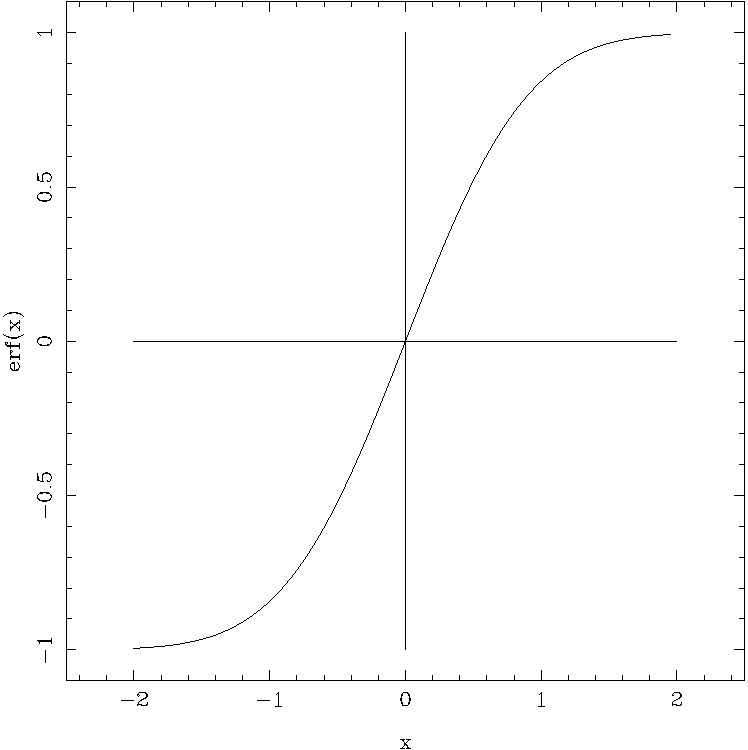
\includegraphics[width=2.0in]{sun194_1}
   \end{center}

% ? Heading for abstract if used.
%   \vspace{10mm}
%   \begin{center}
%      {\Large\bf Abstract}
%   \end{center}
% ? End of heading for abstract.
\end{latexonly}

%  HTML documentation header.
%  ==========================
\begin{htmlonly}
   \xlabel{}
   \begin{rawhtml} <H1> \end{rawhtml}
      \stardoctitle\\
      \stardocversion\\
      \stardocmanual
   \begin{rawhtml} </H1> \end{rawhtml}

% ? Add picture here if required.
   \begin{figure}[h]
      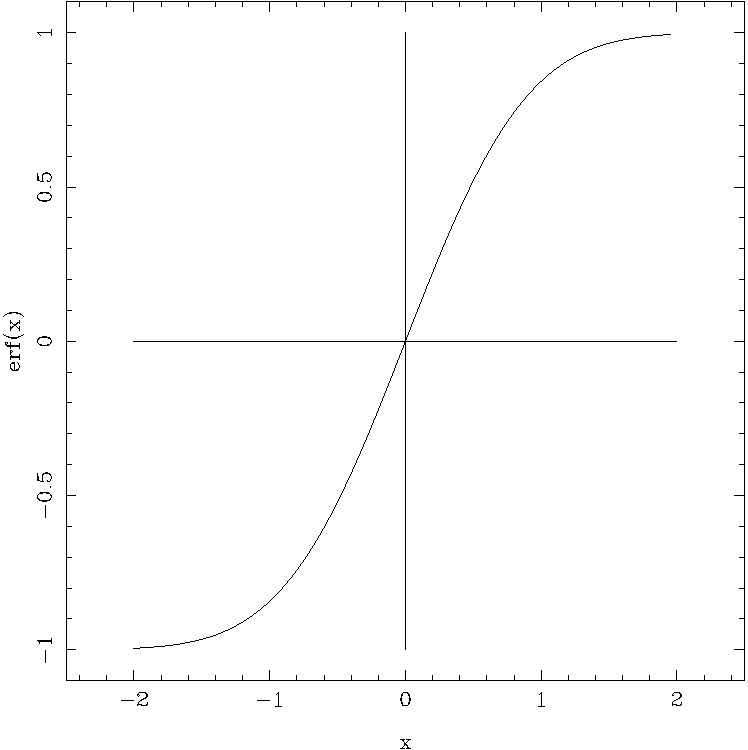
\includegraphics[width=2.0in]{sun194_1}
   \end{figure}
% ? End of picture

   \begin{rawhtml} <P> <I> \end{rawhtml}
   \stardoccategory\ \stardocnumber \\
   \stardocauthors \\
   \stardocdate
   \begin{rawhtml} </I> </P> <H3> \end{rawhtml}
      \htmladdnormallink{CCLRC}{http://www.cclrc.ac.uk} /
      \htmladdnormallink{Rutherford Appleton Laboratory}
                        {http://www.cclrc.ac.uk/ral} \\
      \htmladdnormallink{Particle Physics \& Astronomy Research Council}
                        {http://www.pparc.ac.uk} \\
   \begin{rawhtml} </H3> <H2> \end{rawhtml}
      \htmladdnormallink{Starlink Project}{http://www.starlink.ac.uk/}
   \begin{rawhtml} </H2> \end{rawhtml}
   \htmladdnormallink{\htmladdimg{source.gif} Retrieve hardcopy}
      {http://www.starlink.ac.uk/cgi-bin/hcserver?\stardocsource}\\

%  HTML document table of contents.
%  ================================
%  Add table of contents header and a navigation button to return to this
%  point in the document (this should always go before the abstract \section).
  \label{stardoccontents}
  \begin{rawhtml}
    <HR>
    <H2>Contents</H2>
  \end{rawhtml}
  \htmladdtonavigation{\htmlref{\htmladdimg{contents_motif.gif}}
        {stardoccontents}}

% ? New section for abstract if used.
%  \section{\xlabel{abstract}Abstract}
% ? End of new section for abstract
\end{htmlonly}

% -----------------------------------------------------------------------------
% ? Document Abstract. (if used)
%   ==================
% ? End of document abstract
% -----------------------------------------------------------------------------
% ? Latex document Table of Contents (if used).
%  ===========================================
 \newpage
 \begin{latexonly}
   \setlength{\parskip}{0mm}
   \tableofcontents
   \setlength{\parskip}{\medskipamount}
   \markboth{\stardocname}{\stardocname}
 \end{latexonly}
% ? End of Latex document table of contents
% -----------------------------------------------------------------------------
\cleardoublepage
\renewcommand{\thepage}{\arabic{page}}
\setcounter{page}{1}

% -----------------------------------------------------------------------------
\section{\xlabel{introduction}Introduction}

   This is a preliminary version of the PDA library. PDA
   is intended to replace the
\xref{NAG library}{sun28}{}
   in Starlink application code. A number of people are working on this
   project, and as their contributions become available the
   library will slowly approach version 1.0.

   The library is not intended as a service to Starlink users or as a
   full NAG replacement, but some users may find routines in this library
   useful.

   The library is coded in Fortran and has a Fortran 77 binding. Mostly,
   the interface is for double precision, the Fourier transform part
   provides for both double and single precision, and the routines from
   DIERCKX exist only for single precision.

{\em
   The hints for migration from NAG to this library are incomplete.
   Application programmers are encouraged to check these hints and to
   report on their experience in converting applications from NAG to
   this library.

   NAG is a registered trade mark of The Numerical Algorithms Group. In
   this document the term ``NAG library'' refers to the
\htmladdnormallink{NAG Fortran Library}{http://www.nag.co.uk/1h/numeric/FLOLCH}
   and the
\htmladdnormallink{NAG Graphics Library.}{http://www.nag.co.uk/1h/visual/GLGICH}
   Terms like ``NAG format'', ``NAG array'', ``weights used for NAG''
   refer not to any product of The Numerical Algorithms Group, but to
   the data format that Starlink applications use in order to call the
   NAG library. Similarly, terms like ``NAG code'' refer to Starlink
   application code that calls the NAG library, not to the NAG library
   itself.
\/}

% -----------------------------------------------------------------------------

\section{\xlabel{packages_from_which_the_routines_were_obtained}Packages from which the routines were obtained}

   GAMS -- the
\htmladdnormallink{Guide to Available Mathematical Software}
{http://gams.nist.gov/}
   on the World Wide Web -- was used to identify suitable user-callable
   routines, and the source code was retrieved by following `fullsource'
   anchors on the Web. GAMS is an index to individual subroutines from a
   variety of packages, which in turn are located at several different
   repositories, such as NETLIB.

   One major building block of the library is FFTPACK found in NETLIB (at
   Oak Ridge National Laboratory and AT\&T Bell Laboratories).
   It has been stripped down to just the bits needed to serve Starlink
   applications, i.e.\ routines to take the forward and backward FFT
   of a complex or purely real sequence of values. Some extra
   subroutines have also been written to perform N-dimensional FFTs, and
   to convert arrays of Fourier coefficients between NAG and FFTPACK
   formats. Also, a double precision version has been created.

   Most routines are from the SLATEC library -- a large Public Domain
   library -- and retrieved from the CAMSUN repository at the National
   Institute of Standards and Technology (NIST).

   NMS is another Public Domain library at the TIBER repository (also at
   the National Institute of Standards and Technology).
   Some routines are from MINPACK and retrieved from NETLIB. This too is
   a Public Domain package.

   OPT (from NETLIB) is a less homogeneous package. PDA uses two modules:

\begin{itemize}
\item Simann (PDA\_SA) is a Simulated Annealing algorithm written by
   William L.\ Goffe at the University of Southern Mississippi. It can
   be used freely for research, commercial distribution is not allowed.
   Goffe highly recommends to run the
   algorithm with the test problem with different values for the
   parameters, before one tries it on a ``real'' problem. `The experience
   you gain will be quite helpful.'
\item Subplex (PDA\_SUBPLX) is written by Tow Rowan at the University of
   Texas as Austin. It can be used without restrictions.
\end{itemize}

The gridded 2-D polynomial surface fitting
routines PDA\_DB2INK and PDA\_DB2VAL originated from Ronald
Boisvert of the US National Bureau of Standards. They were
part of CMLIB from CAMSUN.

The ungridded 2-D surface fitting routines
PDA\_IDBVIP and PDA\_IDSFFT were originally
module TOMS526 of the TOMS library at NETLIB.

   Some routines are from the DIERCKX library. The author Paul Dierckx
   calls it FITPACK, but in GAMS they have another library of the same
   name. FITPACK should be considered
   as public domain software and consequently it can be used freely for
   research purposes under existing conditions of appropriate referencing.
   It cannot be used for commercial purposes without the author's
   written consent.

   {\em Although the code of the PDA library comes from other sources in
   the Public Domain, problems with the routines should in the first
   instance be taken up with Starlink and not the original authors. If
   there are bugs in PDA, then the first assumption must be that they
   were introduced during the integration of the Public Domain code into
   the PDA library, and that the original authors are not to blame.}

% -----------------------------------------------------------------------------

\section{\xlabel{routine_naming}Routine naming}

   Library routines have lower-case file names, capitalised file names
   are used for auxiliary source code like test programs.

   Routines keep the same name as they have in the package they are
   retrieved from, except that `pda\_' is prepended. Name conflicts are
   usually due to similar versions of routines in different source
   packages. In these cases the latest or best versions are adopted.

% -----------------------------------------------------------------------------

\section{\xlabel{io_and_error_handling}I/O and error handling}

   The terminal I/O and error handling have been reviewed. Since
   Starlink applications will often run under some environment which
   results in them being
   detached from standard Fortran units, these areas have to be
   addressed and made compliant with Starlink methods of message and
   error handling.

   A few of the FFT routines (not the actual FFTPACK routines) have a
   status argument. It is returned as zero if all went well, and as one
   if an error occurred.

   The DIERCKX/NETLIB routines appear not to make terminal output. Error
   handling takes the form of returning to the caller with a diagnostic
   argument set to the appropriate value. These routines therefore have
   not been changed.

   The MINPACK/NETLIB and OPT/NETLIB routines seem to behave similarly.
   Again no change was made to these routines. It may, however, be
   necessary for the calling routine to choose argument values such that
   printing of messages is suppressed.

   There was a STOP statement in PDA\_RMARIN. This would be executed if
   either of the two seeds for initialisation of the random number
   generator were out of range. These seeds are passed by the user to
   the routine PDA\_SA. Instead of printing a message and stopping the
   program, PDA\_SA will now return STATUS equal to 1. STATUS should
   be given as zero.

   The NMS/TIBER routine PDA\_UNCMND was changed so that it does not
   call PDA\_XERROR any more. It would have used this to issue warning
   and error messages. It also returns a diagnostic argument with the
   same information, so that now it is up to the caller to check and
   interpret that value. There remain two STOP statements in the
   PDA\_UNCMND algorithm, in routines PDA\_D1FCND and PDA\_D2FCND. These
   are dummy routines and never actually called.

The surface fitting routines PDA\_DB2INK and PDA\_DB2VAL call a
routine PDA\_DBVAL2. Originally, PDA\_DBVAL2 called XERROR when a
problem was encountered. These calls have been commented out. The
routine now sets variable {\tt IFAIL} appropriately instead. On exit from
PDA\_DB2INK and PDA\_DB2INK, {\tt STATUS} is set to 1 if the
{\tt IFAIL} value indicated that a serious fault had occurred.
{\tt STATUS} must have the
value 0 when the routines are called.

The surface fitting routines PDA\_IDBVIP and PDA\_IDSFFT, together
with their support routines, have been modified to ensure that {\tt STATUS}
is set to 1 if the internal error status variable {\tt ISTAT} indicates
that a problem was encountered.

   The major work in adapting the library to Starlink error reporting is
   to do with the SLATEC/\-CAMSUN routines. These routines also form the
   major part of the library. The SLATEC error handling procedure would
   be to call
\htmlref{PDA\_XERMSG.}{PDA\_XERMSG}
   Depending on the severity level passed to this routine and depending
   on the error report control flag in a global variable, PDA\_XERMSG might
   or might not print messages, and it might or might not execute a
   Fortran STOP statement.

   PDA\_XERMSG has been re-written. It now has an additional integer argument
   in which it returns the a status value of 1. It will
   also call
\xref{EMS\_REP}{ssn4}{EMS\_REP}
   with a message constructed from the library name, routine name, and
   message text passed to PDA\_XERMSG. PDA\_XERMSG will not execute any STOP
   statement, but always return control to the caller. Since level-2
   errors were always considered fatal, routines calling PDA\_XERMSG may need
   to be changed to cope with regaining control after level-2 errors.

   Routines calling PDA\_XERMSG had to be changed to accommodate the extra
   returned argument. They also have to pass that status argument back
   up to their caller. And they must actually return control to their
   caller before running into exceptions that might crash the program.

% -----------------------------------------------------------------------------

\section{\xlabel{machine_dependencies}Machine dependencies}

   SLATEC and NMS encapsulate machine dependencies in the same set of
   two routines.
\htmlref{PDA\_\-I1MACH}{PDA\_I1MACH}
   contains machine-specific integer constants, and
\htmlref{PDA\_D1MACH}{PDA\_D1MACH}
   contains machine-specific double precision constants. Use of these is
   rare, PDA\_I1MACH is mostly asked for the Fortran unit number for printing
   messages. For single precision constants there would be a third
   routine PDA\_R1MACH, which is so far not in the library.

   The versions of PDA\_D/I1MACH from SLATEC are superior to those from NMS.
   They have later revision dates, and they include cases for both DEC
   Alpha IEEE and Sun. In the library two source files exist,
   pda\_d/i1mach.f\_sun4\_Solaris and pda\_d/i1mach.f\_alpha\_OSF1. In
   usual Starlink manner the `makefile' uses the SYSTEM environment
   variable to pick the right source when building the library.

   MINPACK uses the routine PDA\_DPMPAR, which provides a subset of the
   information available from PDA\_D1MACH. PDA\_D1MACH is the preferred
   routine, but both exist in the library. PDA\_DPMPAR was changed to
   call PDA\_D1MACH.

   It is not known how OPT and DIERCKX depend on machine specifics.

% -----------------------------------------------------------------------------

\section{\xlabel{test_programs}Test programs}

   pda\_test.f is a program that calls all user-callable routines in the
   library. The command

\begin{verbatim}
   % f77 pda_test.f libpda.a -L/star/lib `ems_link`
\end{verbatim}

   should succeed. The test consist of the successful linking, and an
   error message indicates that the library is incomplete or has
   inconsistent module names. The compiled program cannot be executed.

   Erfplot.f can be compiled and linked against PDA and PGPLOT. It
   produced the title graph.

\begin{verbatim}
   % f77 Erftest.f libpda.a -L/star/lib `pgplot_link`
   % ./a.out
\end{verbatim}

   For the FFT routines Ffttest.f can be compiled and linked. It has to
   be linked with PDA {\em and\/} NAG. Ffttest.f convolves two
   test arrays by multiplying their Fourier transforms. This is done
   using NAG routines, and then using FFTPACK routines, and the
   differences between the results (together with timings) are
   displayed. Timings are averaged over 2000 convolutions. The commands

\begin{verbatim}
   % f77 Ffttest.f -L/star/lib -lnag `pda_link`
   % ./a.out > temp
   % diff temp Ffttest.out
\end{verbatim}

   should indicate whether the FFT routines work properly. The output
   will not be exactly as in the distributed file, since it depends on
   the platform, CPU load, etc.

   There are various other test routines included in the PDA distribution:
\begin{itemize}
\item {\tt Covartest.f} - Tests PDA\_NSCOR, PDA\_V11 and PDA\_COVMAT.
\item {\tt E02cbfe.f} - Tests PDA\_CHE2R.
\item {\tt Lintest.f} - Tests PDA\_LSQR.
\item {\tt Nonlin2test.f} - Tests PDA\_DQED.
\item {\tt Nonlintest.f} - Tests PDA\_DNLS1E and PDA\_DENORM.
\item {\tt Normtest.f} - Tests PDA\_PPND16.
\item {\tt Randtest.f} - Tests the random number generators.
\item {\tt Simann.f} - Tests PDA\_SA.
\item {\tt Sorttest.f} - Tests the sorting routines.
\item {\tt Subplex.f} - Tests PDA\_SUBPLX.
\item {\tt Sumsl.f} - Tests PDA\_SUMSL.
\item {\tt Sf2dtest.f} - Tests PDA\_DB2INK and PDA\_DB2VAL.
\item {\tt Sf2dtest2.f} - Tests PDA\_IDBVIP and PDA\_IDSFFT.
\end{itemize}

These test programs can be compiled and linked as follows:

\begin{verbatim}
   % f77 -o <prog> <prog>.f -L/star/lib `pda_link`
\end{verbatim}

Some of these test programs write results to standard output. For such
programs the PDA distribution includes a file with name \verb+<prog>.out+
containing a set of ``standard'' results with which your own results can
be compared.

% -----------------------------------------------------------------------------

\section{\label{LINKING}Linking with the library}

   At a Starlink node the library is available as an archive of object
   modules. Since it is intended
   primarily for Starlink application packages, the link command used is
   most probably `alink'. In that case link as follows:

\begin{verbatim}
   % alink a-task.o -L/star/lib `pda_link_adam`
\end{verbatim}

   The library can equally well be used by ordinary programs:

\begin{verbatim}
   % f77 program.f -L/star/lib `pda_link`
\end{verbatim}

   The {\tt pda\_link} and {\tt pda\_link\_adam} scripts results in your
   program being linked with the Starlink Error Message Service
\xref{(EMS).}{ssn4}{}
   When an error report is to
   be made, the library will call EMS\_SETC and EMS\_REP, and you have to
   link your program against a version of these routines.

   If you do not want to link against EMS, then you can provide your own
   replacements for the two EMS routines. Use the following code:

\begin{verbatim}
*  File name might be mymsg.f

      SUBROUTINE EMS_SETC( MESSG )
      CHARACTER * ( * ) MESSG
      WRITE( *, * ) MESSG
      END

      SUBROUTINE EMS_REP( MNAME, MESSG, STATUS )
      CHARACTER * ( * ) MNAME, MESSG
      INTEGER STATUS
      END
\end{verbatim}

   Then link:

\begin{verbatim}
   % f77 program.f mymsg.f -L/star/lib -lpda
\end{verbatim}

   Finally, if your site is not a Starlink site, you can
   customise the library as such to make EMS obsolete. For this you have
   to replace the error handling routine
\htmlref{PDA\_XERMSG}{PDA\_XERMSG}
   in the library. The new code should be

\begin{verbatim}
*  File name would be pda_xermsg.f

      SUBROUTINE PDA_XERMSG( LIBRAR, SUBROU, MESSG, NERR, LEVEL, STATUS )

      CHARACTER * ( * ) LIBRAR, SUBROU, MESSG
      INTEGER NERR, LEVEL
      INTEGER STATUS

      WRITE( *, * ) LIBRAR // '/' // SUBROU // ': ' // MESSG
      STATUS = 1

      END
\end{verbatim}

   You might also modify the link script pda\_link so that it does not
   refer to ems\_link any more and does not execute any awk command:

\begin{verbatim}

#  N.B. the previous line should be blank.
      echo -lpda
\end{verbatim}

% -----------------------------------------------------------------------------

\section{\xlabel{fast_fourier_transform_fft}Fast Fourier transform (FFT)}

   The routines for fast Fourier transform (and their origin) are:

\begin{itemize}

\item \htmlref{PDA\_RFFTI, PDA\_DRFFTI}{PDA\_RFFTI} (FFTPACK/NETLIB)\ \\
   Initialize PDA\_(D)RFFTF and PDA\_(D)RFFTB.
\item \htmlref{PDA\_RFFTF, PDA\_DRFFTF}{PDA\_RFFTF} (FFTPACK/NETLIB)\ \\
   Forward transform of a real periodic sequence.
\item \htmlref{PDA\_RFFTB, PDA\_DRFFTB}{PDA\_RFFTB} (FFTPACK/NETLIB)\ \\
   Backward transform of a real coefficient array.
\item \htmlref{PDA\_CFFTI, PDA\_DCFFTI}{PDA\_CFFTI} (FFTPACK/NETLIB)\ \\
   Initialize PDA\_(D)CFFTF and PDA\_(D)CFFTB.
\item \htmlref{PDA\_CFFTF, PDA\_DCFFTF}{PDA\_CFFTF} (FFTPACK/NETLIB)\ \\
   Forward transform of a complex periodic sequence.
\item \htmlref{PDA\_CFFTB, PDA\_DCFFTB}{PDA\_CFFTB} (FFTPACK/NETLIB)\ \\
   Unnormalised inverse of PDA\_(D)CFFTF.

\item \htmlref{PDA\_R2NAG, PDA\_DR2NAG}{PDA\_R2NAG}\ \\
   Convert real FFTPACK FT to NAG format.
\item \htmlref{PDA\_NAG2R, PDA\_DNAG2R}{PDA\_NAG2R}\ \\
   Convert real NAG FT to FFTPACK format.
\item \htmlref{PDA\_C2NAG, PDA\_DC2NAG}{PDA\_C2NAG}\ \\
   Convert complex FFTPACK FT to NAG format.
\item \htmlref{PDA\_NAG2C, PDA\_DNAG2C}{PDA\_NAG2C}\ \\
   Convert complex NAG FT to FFTPACK format.

\item \htmlref{PDA\_NFFTF, PDA\_DNFFTF}{PDA\_NFFTF}\ \\
   Forward transform of a complex, N-dimensional data array.
\item \htmlref{PDA\_NFFTB, PDA\_DNFFTB}{PDA\_NFFTB}\ \\
   Backward transform of a complex, N-dimensional coefficient array.

\end{itemize}

%    --------------------------------------------------------------------------

\subsection{\xlabel{differences_between_nag_and_fftpack}Differences between NAG and FFTPACK}

\begin{itemize}
\item
   FFTPACK expects and returns data in a different format to NAG.
\item
   FFTPACK includes initialisation routines (PDA\_RFFTI and PDA\_CFFTI) which
   should be called prior to the other routines, but which don't need to be
   called again until the size of the data array changes. There are no
   equivalent NAG initialisation routines. The main NAG FFT routines
   (e.g.\ C06FAF, etc.) do this initialisation each time they are called,
   irrespective of the array size.
\item
   FFTPACK has separate forward and backward transform routines, whereas
   NAG only has forward routines (backward transforms are performed by
   using complex conjugation with the forward transform). This means that
   there is probably no need to supply equivalents to the complex conjugation
   NAG routines (a trivial operation anyway).
\item
   FFTPACK can accept arrays of any length, whereas NAG puts some
   restrictions on the array length (no prime factor larger than 19 allowed
   in the array size, and the total number of prime factors must be less than
   21).
\item
   FFTPACK routines require a differently sized work space array.
\item
   FFTPACK has no error checking.
\end{itemize}

%    --------------------------------------------------------------------------

\subsection{\xlabel{data_formats_for_fftpack_and_nag}Data formats for FFTPACK and NAG}

   This section describes the differences between the way NAG and
   FFTPACK store arrays of Fourier coefficients. In the following, the
   Fourier transform of an array of N data values is represented by a
   sequence of N complex values
   [A0+i*B0], [A1+i*B1], ..., [A(N-1)+i*B(N-1)].

   The differences are basically in the organisation of the Fourier
   coefficients within the returned array, and also in the
   normalisation. The normalisation of the FFTPACK values is such that
   doing a forward transform followed by a backward transform will
   result in the original array values being multiplied by a factor of
   N.

   Routines to do conversions between FFTPACK and NAG formats have been
   added to the library.

%       -----------------------------------------------------------------------

\subsubsection{\xlabel{fourier_transforms_of_sequences_of_purely_real_values}Fourier transforms of sequences of purely real values}

   The relevant NAG routines are C06FAF and C06FBF (the ``Hermitian''
   routines), and the FFTPACK routines are PDA\_DRFFTI, PDA\_DRFFTF and
   PDA\_DRFFTB.
   These routines take advantage of the symmetries present in the Fourier
   transform of a purely real sequence. Only half of the real (A) and
   imaginary (B) terms need to be calculated and stored because the
   other halves are just the same. This means that only half the space
   is required to store the Fourier transform (i.e.\ N elements rather
   than 2*N), and it takes roughly half the time to evaluate. The
   disadvantage is that the resulting Fourier transform array can be
   rather more difficult to use than if all the real and imaginary parts
   are stored explicitly. There are routines
\htmlref{PDA\_DNAG2R}{PDA\_NAG2R} and
\htmlref{PDA\_DR2NAG}{PDA\_R2NAG}
   to do in-situ conversions between NAG and FFTPACK format. Note, each
   of these routines divides the supplied values by SQRT(N), so
   successive calls to PDA\_DR2NAG and PDA\_DNAG2R do not leave the
   original data
   unaffected (they are divided by N). This is done to cancel the effect
   of successive calls of PDA\_DRFFTF and PDA\_DRFFTB which {\em
   multiplies\/} the original data by N.

   The real and imaginary coefficients produced by PDA\_DRFFTF are
   numerically larger than the corresponding C06FAF coefficients by a
   factor of SQRT(N), and are ordered differently in the returned
   arrays. Both routines return A0 (i.e.\ the DC level in the array) in
   element 1. PDA\_DRFFTF then has corresponding real and imaginary terms in
   adjacent elements, whereas C06FAF has all the real terms together,
   followed by all the imaginary terms (in reverse order):

\begin{verbatim}
   PDA_DRFFTF:  A0,    A1, B1,     A2, B2,     A3, B3,   ...
   C06FAF:      A0,    A1, A2, A3, ...,        ..., B3, B2, B1
\end{verbatim}

   The zeroth imaginary term (B0) always has the value zero and so is
   not stored in the array. Care has to be taken about the parity of the
   array size. If it is even, then there is one more real term than
   there are imaginary terms (excluding A0), i.e.\ if N = 10, then the
   coefficients are stored as follows:

\begin{verbatim}
   PDA_DRFFTF:  A0, A1, B1, A2, B2, A3, B3, A4, B4, A5
   C06FAF:      A0, A1, A2, A3, A4, A5, B4, B3, B2, B1
\end{verbatim}

   If N = 9, then the coefficients are stored as follows:

\begin{verbatim}
   PDA_DRFFTF:  A0, A1, B1, A2, B2, A3, B3, A4, B4
   C06FAF:      A0, A1, A2, A3, A4, B4, B3, B2, B1
\end{verbatim}

%       -----------------------------------------------------------------------

\subsubsection{\xlabel{fourier_transforms_of_sequences_of_complex_values}Fourier transforms of sequences of complex values}

   The relevant NAG routine is C06FCF and the FFTPACK routines are
   PDA\_DCFFTI, PDA\_\-DCFFTF and PDA\_DCFFTB. These routines take the Fourier transform
   of a general complex sequence of N values (i.e.\ 2*N real values),
   also returning the Fourier transform in a sequence of N complex
   values. FFTPACK and NAG differ in that FFTPACK stores the real and
   imaginary parts of each complex value in adjacent elements of the
   array, whereas NAG has two separate arrays, one for the real terms
   and one for the imaginary terms. There is also a difference in the
   normalisation of the routines in that the real and imaginary Fourier
   coefficients produced by PDA\_DRFFTF are numerically larger than the
   corresponding C06FAF coefficients by a factor of SQRT(N). There are
   subroutines
\htmlref{PDA\_DNAG2C}{PDA\_NAG2C} and
\htmlref{PDA\_DC2NAG}{PDA\_C2NAG}
   to convert between NAG and FFTPACK format. Successive calls to
   PDA\_DC2NAG and PDA\_DNAG2C will result in the original data being divided by
   N. This is done to cancel the multiplication by N which occurs when
   successive calls to PDA\_DCFFTF and PDA\_DCFFTB are made.

% -----------------------------------------------------------------------------

\subsection{\xlabel{replacing_calls_to_c06faf}Replacing calls to C06FAF}

   C06FAF is the NAG routine for finding the FFT of a one-dimensional
   sequence of real data values. The routine performs a forward
   transform, storing the FFT as a ``Hermitian'' sequence in which only
   half of the real and imaginary terms are kept. The inverse transform
   is obtained by calling C06FBF, which finds the FFT of a one-dimensional
   Hermitian sequence.

   The following steps are involved in replacing C06FAF calls with
   equivalent FFTPACK calls:

\begin{itemize}

\item{\bf Increase the size of the work array}

   The work array passed to the FFT routine needs to be increased in
   size from N elements (for NAG) to 2*N+15 (for FFTPACK).

\item{\bf Replace call to C06FAF with
\htmlref{PDA\_DRFFTF}{PDA\_RFFTF}}

   Replace the call

\begin{verbatim}
      DOUBLE PRECISION X(N), WORK(N)
      CALL C06FAF( X, N, WORK, IFAIL )
\end{verbatim}

   with

\begin{verbatim}
      DOUBLE PRECISION X(N), WORK(2*N+15)
      CALL PDA_DRFFTF( N, X, WORK )
\end{verbatim}

\item{\bf\label{faf3}Add calls to
\htmlref{PDA\_DRFFTI}{PDA\_RFFTI}
if necessary}

   The work array supplied to PDA\_DRFFTF needs initialising before calling
   PDA\_DRFFTF. This is done by calling PDA\_DRFFTI:

\begin{verbatim}
      DOUBLE PRECISION WORK(2*N+15)
      CALL PDA_DRFFTI( N, WORK )
\end{verbatim}

   There is no need to re-initialise WORK if the value of N has not
   changed since the previous call to PDA\_DRFFTI (and if the contents of the
   work array have not been altered). No harm will occur (except for
   significant slowing down of execution) if the WORK array is
   unnecessarily re-initialised, but it is a good idea to include some
   logic to prevent this.

\item{\bf Convert output (frequency domain) data to NAG format}

   Compared to the Fourier coefficients created by NAG, those created
   by FFTPACK are stored in a different order in the output array and
   are normalised differently. You can either modify your application to
   use the FFTPACK format throughout, or call
   the
\htmlref{PDA\_DR2NAG}{PDA\_R2NAG}
   routine to convert the FFTPACK results into NAG format.

\begin{verbatim}
      DOUBLE PRECISION X(N)
      CALL PDA_DR2NAG( N, X )
\end{verbatim}

   where X is the output from PDA\_DRFFTF. On return, X holds a NAG-style
   Hermitian sequence.

\end{itemize}

%    --------------------------------------------------------------------------

\subsection{\xlabel{replacing_calls_to_c06fbf}Replacing calls to C06FBF}

   C06FBF is the NAG routine for finding the FFT of a one-dimensional
   Hermitian sequence such as created by C06FAF. The routine performs a
   forward transform, but it is usually used to perform an inverse
   transform by preceeding it with a call to C06GBF to form the complex
   conjugates of the input (frequency domain) data.

   The following steps are involved in replacing C06FBF calls with
   equivalent FFTPACK calls:

\begin{itemize}

\item{\bf Convert input (frequency domain) data to FFTPACK format}

   Compared to the Hermitian sequences created by NAG, those created by
   FFTPACK are stored in a different order and are normalised
   differently. You can either modify your application to use the
   FFTPACK format throughout, or call the
\htmlref{PDA\_DNAG2R}{PDA\_NAG2R}
   routine to convert the supplied NAG format data into the
   equivalent FFTPACK format data:

\begin{verbatim}
      DOUBLE PRECISION X(N)
      CALL PDA_DNAG2R( N, X )
\end{verbatim}

   where X is the supplied NAG-style data. On return, X holds the
   FFTPACK-style data, ready for use by PDA\_DRFFTB. If this call is made,
   the values returned by PDA\_DRFFTB will have the same normalisation as the
   original data supplied to PDA\_DRFFTF.

\item{\bf Increase the size of the work array}

   The work array passed to the FFT routine needs to be increased in
   size from N elements (for NAG) to 2*N+15 (for FFTPACK).

\item{\bf Replace call to C06FBF and C06GBF with
\htmlref{PDA\_DRFFTB}{PDA\_RFFTB}}

   Replace the two calls:

\begin{verbatim}
      DOUBLE PRECISION X(N), WORK(N)
      CALL C06GBF( X, N, IFAIL )
      CALL C06FBF( X, N, WORK, IFAIL )
\end{verbatim}

   where X is in NAG format, with

\begin{verbatim}
      DOUBLE PRECISION X(N), WORK(2*N+15)
      CALL PDA_DRFFTB( N, X, WORK )
\end{verbatim}

   where X is in FFTPACK format.

\item{\bf Add calls to
\htmlref{PDA\_DRFFTI}{PDA\_RFFTI}
   if necessary}

   The work array supplied to PDA\_DRFFTB needs initialising before calling
   PDA\_DRFFTB. This is done by calling PDA\_DRFFTI:

\begin{verbatim}
      DOUBLE PRECISION WORK(2*N+15)
      CALL PDA_DRFFTI( N, WORK )
\end{verbatim}

   There is no need to re-initialise WORK if the value of N has not
   changed since the previous call to PDA\_DRFFTI (and if the contents of the
   work array have not been altered).

\end{itemize}

%    --------------------------------------------------------------------------

\subsection{\xlabel{replacing_calls_to_c06fcf}Replacing calls to C06FCF}

   C06FCF is the NAG routine for finding the FFT of a one-dimensional
   sequence of complex data values. The routine performs a forward
   transform. To do an inverse transform the complex conjugate of the
   input data is taken before calling C06FCF (using C06GCF), and the
   complex conjugate of the output data is taken on return from C06FCF.

   The steps involved in replacing C06FCF calls with
   equivalent FFTPACK calls are listed separately for forward and
   inverse transforms.

%       -----------------------------------------------------------------------

\subsubsection{\xlabel{forward_transforms}Forward transforms}

\begin{itemize}

\item{\bf Re-organise the input (spatial domain) data}

   The NAG routine expects real and imaginary parts in separate arrays,
   whereas FFTPACK expects them in the same array, with corresponding
   real and imaginary values in adjacent elements. If the application
   can be changed to supply the input data in this format, so well and
   good. Otherwise you will have to have an extra work array in which to
   hold the input (and output) data in FFTPACK format. You would convert
   the supplied input data using code such as:

\begin{verbatim}
      DOUBLE PRECISION X( N ), Y( N ), C( 2*N )
      DO J = 1, N
         I = 2*J
         C( I - 1 ) = X( J )
         C( I ) = Y( J )
      END DO
\end{verbatim}

   or

\begin{verbatim}
      DOUBLE PRECISION X( N ), Y( N ), C( 2, N )
      DO J = 1, N
         C( 1, J ) = X( J )
         C( 2, J ) = Y( J )
      END DO
\end{verbatim}

   where the X and Y arrays hold the supplied data, C is a work array,
   and N is the number of data points.

\item{\bf Increase the size of the work array}

   The work array passed to the FFT routine needs to be increased in
   size from N elements (for NAG) to 4*N+15 (for FFTPACK).

\item{\bf Replace call to C06FCF with
\htmlref{PDA\_DCFFTF}{PDA\_CFFTF}}

   Replace the call

\begin{verbatim}
      DOUBLE PRECISION X(N), Y(N), WORK(N)
      CALL C06FCF( X, Y, N, WORK, IFAIL )
\end{verbatim}

   with

\begin{verbatim}
      DOUBLE PRECISION C(2*N), WORK(4*N+15)
      CALL PDA_DCFFTF( N, C, WORK )
\end{verbatim}

\item{\bf Add calls to
\htmlref{PDA\_DCFFTI}{PDA\_CFFTI}
   if necessary}

   The work array supplied to PDA\_DCFFTF needs initialising before calling
   PDA\_DCFFTF. This is done by calling PDA\_DCFFTI:

\begin{verbatim}
      DOUBLE PRECISION WORK( 4*N+15 )
      CALL PDA_DCFFTI( N, WORK )
\end{verbatim}

   There is no need to re-initialise WORK if the value of N has not
   changed since the previous call to PDA\_DCFFTI (and if the contents of the
   work array have not been altered). No harm will occur (except for
   significant slowing down of execution) if the WORK array is
   unnecessarily re-initialised, but it is a good idea to include some
   logic to prevent this.

\item{\bf Convert output (frequency domain) data to NAG format}

   The Fourier coefficients created by FFTPACK are stored in a single
   array and are not normalised, whereas NAG stores them in two arrays
   and normalises them. You can either modify the way your application
   to use the FFTPACK format instead of the NAG format, or call the
\htmlref{PDA\_DC2NAG}{PDA\_C2NAG}
   routine to convert the FFTPACK results into NAG format.

\begin{verbatim}
      DOUBLE PRECISION X(N), Y(N), C(2*N)
      CALL PDA_DC2NAG( N, C, X, Y )
\end{verbatim}

   where C is the output from PDA\_DCFFTF, and X and Y hold the corresponding
   real and imaginary coefficients as returned by C06FCF.

   \end{itemize}

%       -----------------------------------------------------------------------

\subsubsection{\xlabel{inverse_transforms}Inverse transforms}

\begin{itemize}

\item{\bf Convert input (frequency domain) data to FFTPACK format}

   If you choose not to modify your application to use FFTPACK data
   format throughout, you can instead do all the conversions just
   before (and after) calling the FFTPACK routines. So, if your
   application supplied frequency domain data in NAG format, first
   convert it to FFTPACK format using the
\htmlref{PDA\_DNAG2C}{PDA\_NAG2C}
   routine:

\begin{verbatim}
      DOUBLE PRECISION X(N), Y(N), C(2*N)
      CALL PDA_DNAG2C( N, X, Y, C )
\end{verbatim}

   where C is an additional work array used to hold the FFTPACK format
   data, ready for use by PDA\_DCFFTB. X and Y are the supplied frequency
   domain data in NAG format. If this call to PDA\_DC2NAG is made, the values
   returned by PDA\_DCFFTB will have the same normalisation as the original
   data supplied to PDA\_DCFFTF.

\item{\bf Increase the size of the work array}

   The work array passed to the FFT routine needs to be increased in
   size from N elements (for NAG) to 4*N+15 (for FFTPACK).

\item{\bf Replace call to C06FCF and C06GCF with
\htmlref{PDA\_DCFFTB}{PDA\_CFFTB}}

   Using NAG, the inverse transform is usually done by the three calls:

\begin{verbatim}
      CALL C06GCF( Y, N, IFAIL )
      CALL C06FCF( X, Y, N, WORK, IFAIL )
      CALL C06GCF( Y, N, IFAIL )
\end{verbatim}

   These three calls should be replaced by the single call:

\begin{verbatim}
      CALL PDA_DCFFTB( N, C, WORK )
\end{verbatim}

   where C is the array into which the X and Y arrays have been converted
   using the method of the previous section.

\item{\bf Add calls to
\htmlref{PDA\_DCFFTI}{PDA\_CFFTI}
   if necessary}

   The WORK array passed to PDA\_DCFFTB should be initialised using
   PDA\_DCFFTI before calling PDA\_DCFFTB. Once the array has been
   initialised it can be used in multiple calls to PDA\_DCFFTF and
   PDA\_DCFFTB so long as they all have the same value for N.

\item{\bf Re-organise the output (spatial domain) data}

   NAG puts the spatial domain results into two arrays (one real, one
   imaginary), whereas FFTPACK puts them into one. You can either
   modify your application to use the FFTPACK format or convert the
   FFTPACK results into NAG-style results using code such as:

\begin{verbatim}
      DOUBLE PRECISION X( N ), Y( N ), C( 2*N )
      DO J = 1, N
         I = 2*J
         X( J ) = C( I - 1 )
         Y( J ) = C( I )
      END DO
\end{verbatim}

   or

\begin{verbatim}
      DOUBLE PRECISION X( N ), Y( N ), C( 2, N )
      DO J = 1, N
         X( J ) = C( 1, J )
         Y( J ) = C( 2, J )
      END DO
\end{verbatim}

\end{itemize}

%    --------------------------------------------------------------------------

\subsection{\xlabel{replacing_calls_to_c06fjf}\label{m_c06fjf}Replacing calls to C06FJF}

   C06FJF is the NAG routine for finding the FFT of an N-dimensional
   array of complex data values. The routine performs a forward
   transformation. To do an inverse transform the complex conjugate of
   the input data is taken before calling C06FJF (using C06GCF), and the
   complex conjugate of the output data is taken on return from C06FJF.

   There are no equivalent routines in FFTPACK as found in NETLIB.
   PDA\_DNFFTF and PDA\_DNFFTB have been written, which do the equivalent of
   C06FJF. These routines are a bit different to genuine FFTPACK
   routines in that they do not need any initialisation, and use NAG
   format rather than native FFTPACK format for complex data arrays and
   Fourier coefficient arrays. Consequently, replacing C06FJF is a bit
   easier than replacing the one-dimensional routines.

   The steps involved in replacing C06FJF calls with
   equivalent FFTPACK calls are listed separately for forward and
   inverse transforms.

%       -----------------------------------------------------------------------

\subsubsection{\xlabel{forward_transforms}Forward transforms}

\begin{itemize}

\item{\bf Increase the size of the work array}

   The work array passed to the FFT routine needs to be increased in
   size from 3*MAXDIM elements (for NAG) to 6*MAXDIM+15 (for FFTPACK).
   Here, MAXDIM is the size of the largest array dimension.

\item{\bf Replace call to C06FJF with
\htmlref{PDA\_DNFFTF}{PDA\_NFFTF}}

   Replace the call

\begin{verbatim}
      DOUBLE PRECISION X(N), Y(N), WORK( 3*MAXDIM )
      INTEGER ND( NDIM )
      CALL C06FJF( NDIM, ND, N, X, Y, WORK, LWORK, IFAIL )
\end{verbatim}

   with

\begin{verbatim}
      DOUBLE PRECISION X(N), Y(N), WORK( 6*MAXDIM + 15 )
      INTEGER ND( NDIM )
      CALL PDA_DNFFTF( NDIM, ND, X ,Y, WORK, ISTAT )
      IF( ISTAT .NE. 0 ) THEN
         This means that NDIM was either less than 1 or greater than 20.
         Report a programming error!
      END IF
\end{verbatim}

\end{itemize}

%       -----------------------------------------------------------------------

\subsubsection{\xlabel{inverse_transforms}Inverse transforms}

\begin{itemize}

\item{\bf Increase the size of the work array}

   The work array passed to the FFT routine needs to be increased in
   size from 3*MAXDIM elements (for NAG) to 6*MAXDIM+15 (for FFTPACK).
   Here, MAXDIM is the size of the largest array dimension.

\item{\bf Replace call to C06FJF and C06GCF with
\htmlref{PDA\_DNFFTB}{PDA\_NFFTB}}

   Using NAG, the inverse transform is usually done by the three calls:

\begin{verbatim}
      CALL C06GCF( Y, N, IFAIL )
      CALL C06FJF( NDIM, ND, N, X, Y, WORK, LWORK, IFAIL )
      CALL C06GCF( Y, N, IFAIL )
\end{verbatim}

   These three calls should be replaced by the single call:

\begin{verbatim}
      CALL PDA_DNFFTB( NDIM, ND, X ,Y, WORK, ISTAT )
\end{verbatim}

\end{itemize}

%    --------------------------------------------------------------------------

\subsection{\xlabel{replacing_calls_to_c06fuf}Replacing calls to C06FUF}

   C06FUF is the NAG routine for finding the FFT of a two-dimensional
   sequence of complex data values. There is no direct equivalent. Use
   the N-dimensional routines instead (with N = 2). See
\htmlref{C06FJF.}{m_c06fjf}

%    --------------------------------------------------------------------------

\subsection{\xlabel{replacing_calls_to_c06gbf_and_c06gcf}Replacing calls to C06GBF and C06GCF}

   The complex conjugation NAG routines C06GBF and C06GCF should no
   longer be needed since separate routines are provided within FFTPACK
   for doing inverse transformation.

% -----------------------------------------------------------------------------

\section{\xlabel{one-dimensional_interpolation_and_fitting,_splines}One-dimensional
Interpolation and Fitting, Splines}

   The routines for this sort of application (and their origins) are:

\begin{itemize}

\item \htmlref{PDA\_BSPDOC}{PDA\_BSPDOC} (SLATEC/CAMSUN)\ \\
   Documentation for BSPLINE, a package of subprograms for working
   with piecewise polynomial functions in B-representation.
\item \htmlref{PDA\_DBINTK}{PDA\_DBINTK} (SLATEC/CAMSUN)\ \\
   Compute the B-representation of a spline which interpolates given
   data. The knots must be given.
\item \htmlref{PDA\_DEFC}{PDA\_DEFC} (SLATEC/CAMSUN)\ \\
   Fit a piecewise polynomial curve to discrete data. The piecewise
   polynomials are represented as B-splines. The fitting is done in a
   weighted least squares sense.
\item \htmlref{PDA\_DBVALU}{PDA\_DBVALU} (SLATEC/CAMSUN)\ \\
   Evaluate the B-representation of a B-spline at X for the function
   value or any of its derivatives.
\item \htmlref{PDA\_DBSQAD}{PDA\_DBSQAD} (SLATEC/CAMSUN)\ \\
   Compute the integral of a K-th order B-spline using the
   B-representation.

\item \htmlref{PDA\_CURFIT}{PDA\_CURFIT} (DIERCKX/NETLIB)\ \\
   Determine a smooth spline approximation of degree k to the given
   set of data points. The knots can be given, or can be determined
   by the routine.
\item \htmlref{PDA\_SPLEV}{PDA\_SPLEV} (DIERCKX/NETLIB)\ \\
   Evaluates in a number of points x(i) a spline s(x) of degree k,
   given in its B-spline representation.
\item \htmlref{PDA\_SPLDER}{PDA\_SPLDER} (DIERCKX/NETLIB)\ \\
   Evaluates in a number of points x(i) the derivative of order NU of
   a spline s(x) of degree k, given in its B-spline representation.
\item \htmlref{PDA\_SPLINT}{PDA\_SPLINT} (DIERCKX/NETLIB)\ \\
   Calculates the integral of a spline function s(x) of degree k,
   which is given in its normalised B-spline representation.

\item \htmlref{PDA\_DPLINT}{PDA\_DPLINT} (SLATEC/CAMSUN)\ \\
   Produce the polynomial which interpolates a set of discrete data
   points.
\item \htmlref{PDA\_DPOLVL}{PDA\_DPOLVL} (SLATEC/CAMSUN)\ \\
   Calculate the value of a polynomial and its first NDER derivatives
   where the polynomial was produced by a previous call to PDA\_DPLINT.
\item \htmlref{PDA\_DPOLCF}{PDA\_DPOLCF} (SLATEC/CAMSUN)\ \\
   Compute the coefficients of the polynomial fit (including Hermite
   polynomial fits) produced by a previous call to PDA\_DPLINT.

\item \htmlref{PDA\_DPOLFT}{PDA\_DPOLFT} (SLATEC/CAMSUN)\ \\
   Fit discrete data in a least squares sense by polynomials in one
   variable. Uses weights.
\item \htmlref{PDA\_DP1VLU}{PDA\_DP1VLU} (SLATEC/CAMSUN)\ \\
   Use the coefficients generated by PDA\_DPOLFT to evaluate the
   polynomial fit of degree L, along with the first NDER of its
   derivatives, at a specified point.
\item \htmlref{PDA\_DPCOEF}{PDA\_DPCOEF} (SLATEC/CAMSUN)\ \\
   Convert the PDA\_DPOLFT coefficients to Taylor series form.

\end{itemize}

%    --------------------------------------------------------------------------

\subsection{\xlabel{b-splines}B-splines}

   E01BAF finds the interpolating cubic spline interpolant f(x) for a
   set of points (x,y). The interpolant is evaluated with E02BBF,
   evaluated with
   derivatives by E02BCF, and integrated by E02BDF. PDA\_DBINTK
   does this, the order of the splines can be changed as well. This
   routine needs to be given the knots, while E01BAF set them itself.
   Evaluation of the interpolant and its derivatives is done by
   PDA\_DBVALU, integration by PDA\_DBSQAD.

   E02BAF finds the fitting cubic spline f(x) for a set of points and
   weights (x,y,w). The interior knots 5 ... n+3 must be given and are
   fixed. The function is evaluated with E02BBF, with derivatives by
   E02BCF, and integrated with E02BDF. PDA\_DEFC does this. All knots must be
   given, not just the interior ones.
   Instead of weights PDA\_DEFC takes standard deviations (x,y,sigma) and uses
   1/sigma as weight. Evaluation of the function and its derivatives is
   done by PDA\_DBVALU, integration by PDA\_DBSQAD.

   E02BBF and E02BCF evaluate an interpolating or fitting cubic spline
   and its derivatives. They follow a call to E01BAF or E02BAF.
   This function is taken over by PDA\_DBVALU.
   E02BDF integrates an interpolating or fitting cubic spline. It
   follows a call to E01BAF or E02BAF. This function is taken over by
   PDA\_DBSQAD.

   E02BEF finds the fitting cubic spline f(x) for a set of points and
   weights (x,y,w). The knots are located automatically. The function is
   evaluated with E02BBF, with derivatives by E02BCF, and integrated
   with E02BDF. PDA\_CURFIT (from the DIERCKX package) solves this problem.
   While the other routines are from SLATEC and for double precision,
   PDA\_CURFIT is for single precision. Hence, PDA\_SPLEV, PDA\_SPLDER
   and PDA\_SPLINT should be used to evaluate the spline, its n-th derivative,
   and its integral.

%    --------------------------------------------------------------------------

\subsection{\xlabel{ordinary_polynomials}Ordinary polynomials}

   E02ADF finds the fitting Chebyshev series minimising r.m.s.\ The
   Chebyshev series is equivalent to an ordinary polynomial, but cannot
   be extrapolated. The
   polynomial is evaluated by E02AEF or E02AKF. In the latter
   routine the Chebyshev coefficients can be one column of an array.
   It will also take the real-world x argument instead of the normalised
   x-bar argument within the range $-$1 ... +1.

   In this library, PDA\_DPOLFT fits an ordinary polynomial as a sum of
   orthogonal polynomials. The representation returned is somewhat
   special. It can be converted to coefficients of a Taylor series with
   PDA\_DPCOEF or directly evaluated with PDA\_DP1VLU. PDA\_DP1VLU will
   return in one call as many derivatives as requested.

%    --------------------------------------------------------------------------

\subsection{\xlabel{replacing_calls_to_e01baf}\label{m_e01baf}Replacing calls to E01BAF}

   The SLATEC equivalent of this routine is
\htmlref{PDA\_DBINTK}{PDA\_DBINTK}
   with order K = 4. The NAG code would look like

\begin{verbatim}
      INTEGER M, IFAIL
      DOUBLE PRECISION X(M), Y(M), T(M+4), C(M+4), WRK(6*M+16)
      IFAIL = 1
      CALL E01BAF( M, X, Y, T, C, M+4, WRK, 6*M+16, IFAIL )
      IF ( IFAIL .NE. 0 ) THEN
         An error has occurred
      END IF
\end{verbatim}

   While the size of the coefficient vector can be reduced to M for
   PDA\_DBINTK, you now need two work spaces.
   The major difference is that PDA\_DBINTK needs to be given the knots. So
   you have to calculate them in the same way as E01BAF would have done.
   The handling of the status is different.

\begin{verbatim}
      INTEGER I, K, M, IFAIL
      PARAMETER ( K = 4 )
      DOUBLE PRECISION X(M), Y(M), T(M+K), C(M)
      DOUBLE PRECISION WRK1( (2*K-1)*M ), WRK2( 2*K )
      DO 1 I = 1, K
         T(I)   = X(1)
         T(M+I) = X(M)
    1 CONTINUE
      DO 2 I = K+1, M
         T(I) = X(I-K/2)      ! Note: K is even
    2 CONTINUE
      IFAIL = 0
      CALL PDA_DBINTK( X, Y, T, M, K, C, WRK1, WRK2, IFAIL )
      IF ( IFAIL .NE. 0 ) THEN
         An error has occurred
      END IF
\end{verbatim}

%    --------------------------------------------------------------------------

\subsection{\xlabel{replacing_calls_to_e02baf}\label{m_e02baf}Replacing calls to E02BAF}

{\em
   PDA\_DEFC has not yet been used anywhere to replace E02BAF. Thus the
   migration hints given here may contain errors or may be based on
   misunderstandings.
\/}

   The SLATEC equivalent of this routine is
\htmlref{PDA\_DEFC}{PDA\_DEFC}
   with order K = 4. The
   NAG code would look like

\begin{verbatim}
      INTEGER M, N, IFAIL
      DOUBLE PRECISION X(M), Y(M), W(M), T(N+7), C(N+7), SS
      DOUBLE PRECISION WORK1(M), WORK2( 4*(N+7) )
      IFAIL = 1
      CALL E02BAF( M, N+7, X, Y, W, T, WORK1, WORK2, C, SS, IFAIL )
      IF ( IFAIL .NE. 0 ) THEN
         An error has occurred
      END IF
\end{verbatim}

   Here N+7 is the number of knots. Since the order is 4 (cubic), the
   number of interior knots is then N+7$-$8 = N$-$1. N is the number of
   intervals. The interior knots are T(5) ... T(N+3). The weights W are
   reciprocal errors of Y. Although C has a length of N+7 only N+3
   coefficients are returned by E02BAF.

   The interior knots T(5) ... T(N+3) are given arguments, but the
   remaining knots are set by E02BAF and thus returned arguments.

   In PDA\_DEFC the order is K = 4. There are N+K+3 knots T(). T(1) ...
   T(K$-$1) and T(N+5) ... T(N+K+3) are end knots. The next
   inner knots T(K) and T(N+4) are presumably the first and last x
   value. Then T(K+1) ... T(N+3) would be truly interior knots just as
   in the NAG code.

   PDA\_DEFC does not generate knots by itself. Contrary to the NAG code
   above, the first K and last K knots must be calculated before the
   call.

   The size of the work space is more complex to calculate. PDA\_DEFC needs
   the standard deviation in Y instead of the weights SD = 1/W. PDA\_DEFC
   returns a diagnostic J, which should have value J = 1 if no error
   occurred.

\begin{verbatim}
      INTEGER I, J, K, L, M, N, IFAIL
      PARAMETER ( K = 4 )
      PARAMETER ( L = (N+6) * (K+1)  + (N+K+4) * (K+1)
     :              + 2*MAX(M,N+K+3) + N+K+3 + K**2 )
      DOUBLE PRECISION X(M), Y(M), W(M), SD(M)
      DOUBLE PRECISION T(N+K+3), C(N+3)
      DOUBLE PRECISION WORK(L)
      DO 1 I = 1, K
         T(I)     = MIN( X() )
         T(N+3+I) = MAX( X() )
    1 CONTINUE
      DO 2 I = 1, M
         SD(I) = 1D0 / W(I)
    2 CONTINUE
      IFAIL = 0
      CALL PDA_DEFC( M, X, Y, SD, K, N+K+3, T, 1, J, C, L, WORK, IFAIL )
      IF ( J .NE. 1 .OR. IFAIL .NE. 0 ) THEN
         An error has occurred
      END IF
\end{verbatim}

%    --------------------------------------------------------------------------

\subsection{\xlabel{replacing_calls_to_e02bbf}Replacing calls to E02BBF}

   The equivalent of this routine in SLATEC is
\htmlref{PDA\_DBVALU}{PDA\_DBVALU}
   with the requested
   derivative being zero and the order being K = 4 for a cubic spline.
   The NAG code would look like

\begin{verbatim}
      INTEGER N, IFAIL
      DOUBLE PRECISION T(N+7), C(N+7), X, S
      IFAIL = 1
      CALL E02BBF( N+7, T, C, X, S, IFAIL )
      IF ( IFAIL .NE. 0 ) THEN
         An error has occurred
      END IF
\end{verbatim}

   Here N, T and C are the same as in
\htmlref{E02BAF.}{m_e02baf}
   If T and C originate from
   a call to
\htmlref{E01BAF}{m_e01baf}
   then for N+7 read M+4 with M the number of data
   points given to the interpolation.

   PDA\_DBVALU is a function rather than a subroutine. The dimension passed
   to PDA\_DBVALU is not that of T, but that of C, i.e.\ N+3 (or M after
   interpolation). PDA\_DBVALU returns the value of any derivative, the fifth
   argument is zero so that it returns the function value itself. INVB
   must be given 1 in the first call. For several evaluations of the
   same spline it should not be changed between calls. It is changed by
   PDA\_DBVALU. So if PDA\_DBVALU is called in a DO loop, the statement INVB = 1
   is typically before and outside the loop.

\begin{verbatim}
      INTEGER INVB, K, N
      PARAMETER ( K = 4 )
      DOUBLE PRECISION T(N+K+3), C(N+3), X, S
      DOUBLE PRECISION WORK(3*K)
      DOUBLE PRECISION PDA_DBVALU
      INVB = 1
      IFAIL = 0
      S = PDA_DBVALU( T, C, N+3, K, 0, X, INVB, WORK, IFAIL )
      IF ( IFAIL .NE. 0 ) THEN
         An error has occurred
      END IF
\end{verbatim}

%    --------------------------------------------------------------------------

\subsection{\xlabel{replacing_calls_to_e02bcf}Replacing calls to E02BCF}

{\em E02BCF has not yet been replaced anywhere. Thus the
   migration hints given here may contain errors or may be based on
   misunderstandings.\/}

   The equivalent of this routine in SLATEC is
\htmlref{PDA\_DBVALU.}{PDA\_DBVALU}
   Several calls are
   necessary, one for each derivative. For the function value itself set
   the number of derivative to zero. The order is K = 4 for a cubic
   spline. The NAG code would look like

\begin{verbatim}
      INTEGER LEFT, N, IFAIL
      DOUBLE PRECISION T(N+7), C(N+7), X, S(O:3)
      IFAIL = 1
      CALL E02BCF( N+7, T, C, X, LEFT, S, IFAIL )
      IF ( IFAIL .NE. 0 ) THEN
         An error has occurred
      END IF
\end{verbatim}

   Here N, T and C are the same as in
\htmlref{E02BAF.}{m_e02baf}
   If T and C originate from
   a call to
\htmlref{E01BAF}{m_e01baf}
   then for N+7 read M+4 with M the number of data
   points given to the interpolation. S(I) returns the I-th derivative.
   In the case that X coincides with a knot and the derivatives are not
   continuous at that knot, LEFT is used to decide which side of the
   knot to use.

   PDA\_DBVALU is a function rather than a subroutine. The dimension passed
   to PDA\_DBVALU is not that of T, but that of C, i.e.\ N+3 (or M after
   interpolation). PDA\_DBVALU returns the value of any derivative, as
   specified in the fifth argument.

   There is no equivalent to
   the LEFT parameter in NAG. PDA\_DBVALU returns right limiting values,
   except at the right end point.

   INVB must be given 1 in the first call. For several evaluations of
   the same spline it should not be changed between calls. It is changed
   by PDA\_DBVALU. So if PDA\_DBVALU is called in a DO loop, the statement INVB =
   1 is typically before and outside the loop. In the code below, IFAIL
   is reset inside the DO loop. Assuming that an error will quit the
   loop, the IFAIL = 0 statement could be before and outside the DO loop
   as well.

\begin{verbatim}
      INTEGER INVB, I, K, N
      PARAMETER ( K = 4 )
      DOUBLE PRECISION T(N+K+3), C(N+3), X, S(0:K-1)
      DOUBLE PRECISION WORK(3*K)
      DOUBLE PRECISION PDA_DBVALU
      INVB = 1
      DO 1 I = 0, K-1
         IFAIL = 0
         S(I) = PDA_DBVALU( T, C, N+3, K, I, X, INVB, WORK, IFAIL )
         IF ( IFAIL .NE. 0 ) THEN
            An error has occurred
         END IF
    1 CONTINUE
\end{verbatim}

%    --------------------------------------------------------------------------

\subsection{\xlabel{replacing_calls_to_e02bdf}Replacing calls to E02BDF}

{\em
   PDA\_DBSQAD has not yet been used anywhere to replace E02BDF. Thus the
   migration hints given here may contain errors or may be based on
   misunderstandings.
\/}

   The equivalent of this routine in SLATEC is
\htmlref{PDA\_DBSQAD.}{PDA\_DBSQAD}
   The NAG code
   would look like

\begin{verbatim}
      INTEGER N, IFAIL
      DOUBLE PRECISION T(N+7), C(N+7), DEFINT
      IFAIL = 1
      CALL E02BDF( N+7, T, C, DEFINT, IFAIL )
      IF ( IFAIL .NE. 0 ) THEN
         An error has occurred
      END IF
\end{verbatim}

   Here N, T and C are the same as in
\htmlref{E02BAF.}{m_e02baf}
   If T and C originate from
   a call to
\htmlref{E01BAF}{m_e01baf}
   then for N+7 read M+4 with M the number of data
   points given to the interpolation. DEFINT returns the integral over
   the whole x range where the spline is defined. This is from T(4) to
   T(N+4), which are most probably the smallest and largest X used in
   the fit or interpolation.

   The dimension passed
   to PDA\_DBSQAD is not that of T, but that of C, i.e.\ N+3 (or M after
   interpolation). PDA\_DBSQAD calculates the integral for any interval
   on which the spline is defined. For the same interval as in the NAG
   code, the two limiting knots are given to PDA\_DBSQAD.

\begin{verbatim}
      INTEGER K, N
      PARAMETER ( K = 4 )
      DOUBLE PRECISION T(N+K+3), C(N+3), DEFINT
      DOUBLE PRECISION WORK(3*K)
      CALL PDA_DBSQAD( T, C, N+3, K, T(4), T(N+4), DEFINT, WORK, IFAIL )
      IF ( IFAIL .NE. 0 ) THEN
         An error has occurred
      END IF
\end{verbatim}

%    --------------------------------------------------------------------------

\subsection{\xlabel{replacing_calls_to_e02bef}Replacing calls to E02BEF}

   E02BEF is a more advanced routine than the other NAG spline routines.
   It places knots automatically while fitting a cubic spline. This
   library includes for this case a number of routines from DIERCKX.
\htmlref{PDA\_CURFIT}{PDA\_CURFIT}
   performs the spline approximation with given or
   automatic knots. The fitted function is evaluated with
\htmlref{PDA\_SPLEV,}{PDA\_SPLEV}
   its
   derivatives with
\htmlref{PDA\_SPLDER,}{PDA\_SPLDER}
   its integral with
\htmlref{PDA\_SPLINT.}{PDA\_SPLINT}
   The routines exist
   only for single precision arguments.

   These routines are so far unused, so there are no migration hints.

%    --------------------------------------------------------------------------

\subsection{\xlabel{replacing_calls_to_e02adf}\label{m_e02adf}Replacing calls to E02ADF}

   Superficially, the equivalent SLATEC routine is
\htmlref{PDA\_DPOLFT.}{PDA\_DPOLFT}
   Since NAG
   has no routine to do a polynomial extrapolation,
   Figaro usurped this routine with a peculiar set of weights
   and very few degrees of freedom to extrapolate a polynomial. Although
   PDA\_DPOLFT can be used even in that case, it is
\htmlref{PDA\_DPLINT}{PDA\_DPLINT}
   that is
   intended for polynomial interpolation.

   The NAG code would look like

\begin{verbatim}
      INTEGER I, M, K, NROWS, IFAIL
      DOUBLE PRECISION X(M), Y(M), W(M)
      DOUBLE PRECISION WORK1(3*M), WORK2( 2*(K+1) )
      DOUBLE PRECISION A1(NROWS,K+1), S(K+1)
      DOUBLE PRECISION A2(K+1)
      IFAIL = 1
      CALL E02ADF( M, K+1, NROWS, X, Y, W, WORK1, WORK2, A1, S, IFAIL )
      IF ( IFAIL .NE. 0 ) THEN
         An error has occurred
      END IF
      DO 1 I = 1, K+1
         A2(I) = A1(K+1,I)
    1 CONTINUE
\end{verbatim}

   Here W are the weights proportional to the reciprocal of the standard
   deviation of Y. A1 returns a matrix of Chebyshev coefficients, one
   set of coefficients for each polynomial degree from 0 to K. The DO
   loop extracts the coefficients for degree K into A2. Note that these
   coefficients form a column rather than a row in A1. S returns the
   r.m.s.\ for the fit of each degree from 0 to K.

   The behaviour of PDA\_DPOLFT is controlled by the given value of EPS,
   passing zero (0D0) makes it perform fits for all degrees from 0 to K.
   EPS is also a returned argument, it returns the r.m.s.\ for
   the highest degree fitted. What degree that was is returned in NDEG.
   An indication of the success is returned in IFAIL1.

   The weights should be proportional to the reciprocal of the variance,
   i.e.\ the square of the weights used for NAG.

   The returned description of the polynomials A3 is rather different
   from the Chebyshev coefficients returned by E02ADF. A3 would be
   passed on to
\htmlref{PDA\_DP1VLU}{PDA\_DP1VLU}
   to evaluate the polynomial or to
\htmlref{PDA\_DPCOEF}{PDA\_DPCOEF}
   to
   convert A3 to coefficients of a Taylor series. A3 contains sufficient
   information to evaluate the polynomial of any degree from 0 to K. The
   desired degree is specified to PDA\_DP1VLU or PDA\_DPCOEF.

   R is a returned vector in which the fit of highest degree is
   evaluated at all given X. Often this may render any further
   evaluation calls obsolete.

\begin{verbatim}
      INTEGER I, M, K, NDEG, IFAIL1, IFAIL2
      DOUBLE PRECISION X(M), Y(M), W(M), W2(M), R(M)
      DOUBLE PRECISION A3( 3*M + 3*(K+1) )
      DOUBLE PRECISION EPS, S(K+1)
      DO 1 I = 1, M
         W2(I) = W(I) * W(I)
    1 CONTINUE
      IFAIL2 = 0
      EPS = 0D0
      CALL PDA_DPOLFT( M, X, Y, W2, K, NDEG, EPS, R, IFAIL1, A3, IFAIL2 )
      IF ( NDEG .NE. K .OR. IFAIL1 .NE. 1 .OR. IFAIL2 .NE. 0 ) THEN
         An error has occurred
      END IF
      DO 2 I = 1, K
         S(I) = 0D0
    2 CONTINUE
      S(K+1) = EPS
\end{verbatim}

%    --------------------------------------------------------------------------

\subsection{\xlabel{replacing_calls_to_e02aef}\label{m_e02aef}Replacing calls to E02AEF}

   The equivalent of this routine in SLATEC is
\htmlref{PDA\_DP1VLU.}{PDA\_DP1VLU}
   The NAG code
   would look like

\begin{verbatim}
      INTEGER I, K, K2, NROWS, IFAIL
      DOUBLE PRECISION A1(NROWS,K+1)
      DOUBLE PRECISION A2(K2+1), XX, XCAP, P
      DO 1 I = 1, K2+1
         A2(I) = A1(K2+1,I)
    1 CONTINUE
      XCAP = ( ( XX - MIN(X()) ) - ( MAX(X()) - XX ) )
     :     / ( MAX(X()) - MIN(X()) )
      IFAIL = 1
      CALL E02AEF( K2+1, A2, XCAP, P, IFAIL )
      IF ( IFAIL .NE. 0 ) THEN
         An error has occurred
      END IF
\end{verbatim}

   Here A1 is the coefficient matrix returned by
\htmlref{E02ADF,}{m_e02adf}
   A2 is the
   column extracted for the required degree. XX is the x value for
   which an evaluation is required, it must be scaled into the range
   $-$1 ... +1, using the original extreme x values passed to E02ADF. P
   returns the function value.

   PDA\_DP1VLU returns any number of derivatives in addition to the function
   value. The second argument specifies how many derivatives are
   required. No scaling of XX is necessary, and no processing of the
   coefficients A3 as returned by
\htmlref{PDA\_DPOLFT.}{PDA\_DPOLFT}

\begin{verbatim}
      INTEGER K, K2, IFAIL
      DOUBLE PRECISION A3( 3*M + 3*(K+1) )
      DOUBLE PRECISION XX, P, DUMMY
      IFAIL = 0
      CALL PDA_DP1VLU( K2, 0, XX, P, DUMMY, A3, IFAIL )
      IF ( IFAIL .NE. 0 ) THEN
         An error has occurred
      END IF
\end{verbatim}

%    --------------------------------------------------------------------------

\subsection{\xlabel{replacing_calls_to_e02akf}Replacing calls to E02AKF}

   E02AKF is similar to
\htmlref{E02AEF}{m_e02aef}
   but provides a different interface.
   Namely, A1 (from
\htmlref{E02ADF)}{m_e02adf}
   and the row length can be given instead of the extraction
   A2. Also XX is given rather than the scaled XCAP. There are no
   detailed migration hints for this routine yet.

%    --------------------------------------------------------------------------

\subsection{\xlabel{replacing_calls_to_genchb2no}Replacing calls to GEN\_CHB2NO}

   This is not a NAG routine, but a routine in
\xref{Figaro's}{sun86}{}
   GEN library. It converts the vector of Chebyshev coefficients into a
   vector of coefficients of an ordinary polynomial. This is
   particularly useful when these are to be written to output files. In
   future the routine will still be needed to read old files that
   contain Chebyshev coefficients.

   This routine is mentioned here really, because it has an equivalent
   in SLATEC named PDA\_\-DPCOEF.
\htmlref{PDA\_DPCOEF}{PDA\_DPCOEF}
   is more general, in that it returns
   coefficients for a Taylor series, i.e.\ a polynomial in (XX-X0) for
   given expansion point X0.

   The old code would look like

\begin{verbatim}
      INTEGER I, K, K2, NROWS
      DOUBLE PRECISION A1(NROWS,K+1)
      DOUBLE PRECISION A2(K2+1), C(K2+1)
      DO 1 I = 1, K2+1
         A2(I) = A1(K2+1,I)
    1 CONTINUE
      CALL GEN_CHB2NO( K2, MIN(X()), MAX(X()), A2, C )
\end{verbatim}

   This would be replaced by

\begin{verbatim}
      INTEGER K, K2, IFAIL
      DOUBLE PRECISION A3( 3*M + 3*(K+1) )
      DOUBLE PRECISION C(K2+1)
      IFAIL = 0
      CALL PDA_DPCOEF( K2, 0D0, C, A3, IFAIL )
      IF ( IFAIL .NE. 0 ) THEN
         An error has occurred
      END IF
\end{verbatim}

   Just in case you are tempted to evaluate the polynomial yourself
   rather than use
\htmlref{PDA\_DP1VLU,}{PDA\_DP1VLU}
   here is a piece of code to get P = f(XX):

\begin{verbatim}
      INTEGER I, K2
      DOUBLE PRECISION XX, P
      DOUBLE PRECISION C(K2+1)
      P = C(K2+1)
      DO 2 I = K2, 1, -1
         P = P * XX
         P = P + C(I)
    2 CONTINUE
\end{verbatim}

% -----------------------------------------------------------------------------
\section{\xlabel{two-dimensional_interpolation_and_fitting}Two-dimensional
Interpolation and Fitting}

The routines for this sort of application are:

\begin{itemize}

\item \htmlref{PDA\_CHE2D}{PDA\_CHE2D}
   PDA\_CHE2D evaluates a 2-dimensional Chebyshev polynomial. A single
   precision version (PDA\_CHE2R) is available.

\item \htmlref{PDA\_BISPEV}{PDA\_BISPEV}
   PDA\_BISPEV evaluates the bivariate spline approximation found by
   PDA\_SURFIT.

\item \htmlref{PDA\_DB2INK}{PDA\_DB2INK}
   PDA\_DB2INK determines a piecewise polynomial function that
   interpolates the two-dimensional gridded data. Users specify
   the polynomial order (degree+1) of the interpolant and
   (optionally) the knot sequence.

   The interpolating  function  is  a  piecewise  polynomial
   represented as a tensor product of one-dimensional  B-splines.

\item \htmlref{PDA\_DB2VAL}{PDA\_DB2VAL}
    PDA\_DB2VAL evaluates  the  tensor product piecewise  polynomial
    interpolant constructed by the routine PDA\_DB2INK, or,
    alternatively evaluates one of its derivatives, at a given point.
    Function values returned are double precision.

\item \htmlref{PDA\_IDBVIP}{PDA\_IDBVIP}
     PDA\_IDBVIP performs bivariate interpolation when the
     the data points are irregularly distributed in the x-y plane.
     Function values returned are single precision.

\item \htmlref{PDA\_IDSFFT}{PDA\_IDSFFT}
     PDA\_IDSFFT performs smooth surface fitting when the data points
     are irregularly distributed in the x-y plane.
     Function values returned are single precision.

\item \htmlref{PDA\_SURFIT}{PDA\_SURFIT}
     PDA\_SURFIT determines a smooth bivariate spline approximation for
     irregularly distributed data.

\end{itemize}


E02DAF calculates a 2-D bi-cubic spline interpolating surface
for points from a regular grid. The routines E02DEF/E02DFF may then
be used to compute values of the spline at the required location.
This approach has has been replaced by using the routine pair PDA\_DB2INK
and PDA\_DB2VAL. No significant change in program performance
was found.

E02SAF provides a 2-D surface fit for data on an
irregular spaced grid. The method employed is that of Renka and
Cline where the grid is used to construct a set of suitably
weighed equiangular triangles that (with appropriate weighting)
describe the surface. The interpolated value of the gridded data
at any point within the grid is extracted by E02SBF. This pair of
routines has been replaced using PDA\_IDBVIP with no significant change
in program performance. During incomplete trials the routine PDA\_IDSFFT
also appeared to give sensible results.

\subsection{\xlabel{replacing_calls_to_e02daf}Replacing calls to E02DAF}

E02DAF can be replaced with the following code.

\begin{verbatim}
*   Declare variables
      INTEGER ID                      ! Specifies use value not differential
      INTEGER IFAIL                   ! Was the surface successfully created?
      INTEGER MXY                     ! Size of the grid
      INTEGER ORD                     ! Order of polynomial used

      DOUBLE PRECISION DVALUE         ! Interpolated value returned
      DOUBLE PRECISION FV1(8,8)       ! Grid Z values
      DOUBLE PRECISION X1(8), Y1(8)   ! X,Y grid locations
      DOUBLE PRECISION XD, YD         ! X,Y coord for interpolation

      DOUBLE PRECISION BCOEF(8,8)     ! Array used by PDA_DB2INK
      DOUBLE PRECISION TX(11),TY(11)  ! Array used by PDA_DB2INK
      DOUBLE PRECISION WORK(168)      ! Array used by PDA_DB2INK

*   Subroutine initial error values.
      IFAIL=0
      STATUS=0

*   Order of polynomial used in this example.
      ORD=3

*   Use value rather than differential.
      ID=0

*   Size of data grid. 8x8 in this instance.
      MXY=8

*   Build the surface fit using the grid contents.
      CALL PDA_DB2INK(X1,MXY,Y1,MXY,FV1,MXY,
     :                ORD,ORD,TX,TY,BCOEF,
     :                WORK,IFAIL,STATUS)


*   If IFAIL=1 then okay to interpolate values.
      IF (IFAIL.EQ.1) THEN

*       Setup evaluation routine.
          IFAIL=0
          CALL PDA_DB2VAL(XD,YD,ID,ID,TX,TY,
     :                    MXY,MXY,ORD,ORD,BCOEF,WORK,
     :                    DVALUE,IFAIL,STATUS)

      END IF
\end{verbatim}

In the example shown the value of the surface fitted is
calculated at a point defined by {\tt XD} and {\tt YD}. The
surface constructed is a 3rd order, polynomial and the value
returned by PDA\_DB2VAL is the surface value not its differential.
The example assumes that the array {\tt FV1()} already contains
values for the data at each of the grid points defined in
arrays {\tt X1} and {\tt Y1}. The size of the work arrays is
determined by the size of the grid required. The variable {\tt
DVALUE} contains the interpolated value.


\subsection{\xlabel{replacing_calls_to_e02saf}Replacing calls to E02SAF}

It has been found in tests that the following code examples adequately
replace calls to E02SAF.

\begin{verbatim}
*  Local Variables:
      INTEGER  ISTAT                   ! Status
      INTEGER  MD                      ! Mode
      INTEGER  NDP                     ! Grid points
      INTEGER  NCP                     ! Not used
      INTEGER  NOP                     ! Size of returned array
      INTEGER  IWK(2500)               ! Workspace
      REAL     WK(640)                 ! Workspace
      REAL     XD(80),YD(80),ZD(80)    ! Surface data
      REAL     XI(1),YI(1)             ! Extrap points
      REAL     ZI(1,1)                 ! Results


*   Set the error flag default values.
      ISTAT=0
      STATUS=0

*   Set mode and the grid positions (for PDA_IDBVIP).
      MD= 1
      NCP=2
      NOP=1

*   Call interpolation subroutine.
      CALL PDA_IDBVIP(MD,NCP,NDP,XD,YD,ZD,NOP,XI,YI,
     :                ZI,IWK,WK,ISTAT,STATUS)
\end{verbatim}

In the example shown, the value of the interpolated surface
at {\tt XI(1),YI(1)} is returned in the variable {\tt ZI(1,1)}.
The surface is constructed using
co-ordinate information from the arrays of {\tt XD()} and {\tt YD()},
and surface values contained in the array {\tt ZD()}. The number
of data points available to define the surface is {\tt NDP}.

If several values are required from locations within the
irregular grid, the mode variable {\tt MD} should for the first
point be set to 1 but may subsequently be 2. This
significantly increases the execution speed. The size of the work
arrays is determined by the size of the grid required.

Alternatively, the routine PDA\_IDSFFT may be used thus:

\begin{verbatim}
      INTEGER  ISTAT                   ! Status
      INTEGER  MD                      ! Mode
      INTEGER  NDP                     ! Grid points
      INTEGER  NCP                     ! Not used
      INTEGER  NXI,NYI                 ! Output gird size
      INTEGER  IWK(2500)               ! Workspace
      REAL     XD(80),YD(80),ZD(80)    ! Surface data
      REAL     XI(1),YI(1)             ! Extrap points
      REAL     ZI(1,1)                 ! Results
      REAL     WK(640)                 ! Workspace

*   Set the error flag default values.
      ISTAT=0
      STATUS=0

*   Set up the grid positions.
      NXI=1
      NYI=1

*   Set mode and the grid positions (for PDA_IDBVIP).
      MD= 1
      NCP=2

*         Call the surface fitting subroutine.
            CALL PDA_IDSFFT(MD,NCP,NDP,XD,YD,ZD,
     :                      NXI,NYI,XI,YI,ZI,IWK,
     :                      WK,ISTAT,STATUS)
\end{verbatim}

In the example shown the surface is constructed from the irregular grid
information contained in arrays {\tt XD()/YD()} (location) and
{\tt ZD()} (surface value). Interpolated values calculated from the
fitted surface are returned in the {\tt ZI()} array at the co-ordinates
specified by the data in the {\tt XI()} and {\tt YI()} arrays.

If several values are required from locations within the
irregular grid, the mode variable {\tt MD} should for the first
point be set to 1 but may subsequently be 2. This
significantly increases the execution speed. The size of the work
arrays is determined by the size of the grid required.

\subsection{\xlabel{replacing_calls_to_e02cbf}Replacing calls to E02CBF}
The routine PDA\_CHE2D (or its single precision equivalent PDA\_CHE2R)
can be used to replace E02CBF. The replacement is straightforward with most
of the arguments being the same, albeit in a slightly different order.

% -----------------------------------------------------------------------------

\section{\xlabel{minimisation}Minimisation}

   The routines for minimisation (or optimisation) in this library are:

\begin{itemize}

\item \htmlref{PDA\_DNLS1}{PDA\_DNLS1} \\
   Minimises the sum of squares of M non-linear functions.

\item \htmlref{PDA\_DNLS1E}{PDA\_DNLS1E} \\
   Minimises the sum of squares of M non-linear functions (easy version).

\item \htmlref{PDA\_DQED}{PDA\_DQED} \\
   Solve bounded nonlinear least squares and nonlinear equations.

\item \htmlref{PDA\_LMDIF1}{PDA\_LMDIF1} (MINPACK/NETLIB)\ \\
   Minimise the sum of the squares of m nonlinear functions in n
   variables, simple interface to PDA\_LMDIF.

\item \htmlref{PDA\_LMDIF}{PDA\_LMDIF} (MINPACK/NETLIB)\ \\
   Minimise the sum of the squares of m nonlinear functions in n
   variables with a modified Levenberg-Marquardt algorithm. Needs
   function only, the Jacobian is calculated by a forward-difference
   approximation.

\item \htmlref{PDA\_UNCMND}{PDA\_UNCMND} (NMS/TIBER)\ \\
   Minimises a smooth non-linear function of n variables. Needs
   function values only.

\item \htmlref{PDA\_SA}{PDA\_SA} (module SIMANN from OPT/NETLIB)\ \\
   Continuous simulated annealing global optimisation algorithm.
   Simple constraints can be specified.

\item \htmlref{PDA\_SUMSL}{PDA\_SUMSL} (module SUMSL from TOMS)\ \\
   Minimises a general unconstrained objective function using
   analytic gradients and a hessian approximation from secant update.

\item \htmlref{PDA\_SUBPLX}{PDA\_SUBPLX} (module SUBPLEX from OPT/NETLIB)\ \\
   Subplex method to solve unconstrained optimisation problems.  The
   method is well suited for optimising objective functions that are
   noisy or are discontinuous at the solution.

\end{itemize}

%    --------------------------------------------------------------------------

\subsection{\xlabel{overview}Overview}

   There are two sorts of minimisation, one is to minimise any old
   function, and one to minimise a sum of squares. The first is more
   general, the least-squares routines are presumably more efficient.
   For the programmer the differences are as follows:

\begin{itemize}
\item
   For a least-squares fit, your merit function is a vector of residuals
   between measurements and current model guess.
   For a general minimisation your merit function is a scalar, basically
   you have to add up the squared residuals within your merit function.
\item
   Perhaps more important is the amount of workspace you have to
   provide to the fit algorithm. In least-squares fits this scales with
   n*m where n is the number of parameters to be fitted and m is the
   number of residuals to be added up (e.g.\ channels in a spectrum).
   m is quite large and depends on the data set at hand. The general
   minimisation does in principle not know that there is a spectrum with
   m pixels, and its workspace scales with the square of n, which is
   more or less constant for any given application.
\item
   Another difference is that least-squares fits tend to return the
   Jacobi matrix, the derivatives of each fit parameter with respect to
   each measurement. This is quite valuable if you want to know the
   variances of the fit parameters and the covariances between them. With
   the general minimisation you would have to work out the Hesse matrix
   and invert it. Which means you have to be able to work out the
   derivatives of you merit function w.r.t.\ to each fit parameter.
\end{itemize}

   Two other issues in choosing minimisation algorithms are whether only
   the merit function can be provided or also first derivatives, and
   whether the fit parameters have to be constrained or not. It appears
   that Starlink applications use mainly unconstrained fits or at most
   simple bounds, i.e.\ hard constant limits on parameters. This library
   contains function-only algorithms, and also the SUMSL algorithm
   which requires both functions and gradients. The only constrainable
   algorithm is the simulated annealing SIMANN.

\begin{itemize}
\item
   PDA\_UNCMND is a general unconstrained minimisation using function values
   only. A quasi-Newton algorithm with line search is used.
\item
   PDA\_LMDIF/PDA\_LMDIF1 is an unconstrained least-squares minimisation using
   residuals only (no derivatives).
   A modified Levenberg-Marquardt algorithm is used, the Jacobian is
   calculated by a forward-difference approximation.
\item
   SIMANN is a simulated annealing algorithm. It uses function values
   only and can be used for non-smooth functions as well. It should also
   have a fair chance of getting out of local minima and going on to
   find the global minimum.
\item
   SUMSL is a general unconstrained minimisation using function values
   and gradients. A trusted regions algorithm is used.
\item
   SUBPLEX is a generalisation and improvement on the Simplex algorithm.
   It should be very robust with any function to minimise. But it should
   also be rather inefficient.
\end{itemize}

%    --------------------------------------------------------------------------

\subsection{\xlabel{replacing_calls_to_e04dgf_and_e04dkf}Replacing calls to E04DGF and E04DKF}

   E04DGF performs an unconstrained minimisation using function
   values and first derivatives, E04DKF is just an auxiliary routine. To
   replace these,
\htmlref{PDA\_UNCMND}{PDA\_UNCMND}
   would be used, which does not make use of
   derivatives.

   The existing NAG code might look as shown below. Two modules are
   involved, one controls the NAG fit routine, the other serves it by
   providing the value and gradient of the merit function (the function
   to be minimised). Information is passed to the merit function in two
   ways. Scalars and constant-size arrays are in a common block, while
   one variable-length array is passed as the USER argument. Its length
   is passed in IUSER. The controlling function may also call the merit
   function directly.

\begin{verbatim}
      SUBROUTINE DOAFIT( ... )
      INTEGER N
      INTEGER IUSER
      INTEGER ITER, IFAIL
      INTEGER IWORK(N+1)
      REAL USER(IUSER)
      DOUBLE PRECISION X(N), FVAL, FGRAD(N)
      DOUBLE PRECISION WORK(13*N)
      EXTERNAL MERIT
  +-  COMMON / ABLOCK / constant-size arrays
  |   CALL MERIT( 0, N, X, FVAL, FGRAD, 0, IUSER, USER )
  |   IFAIL = 1
  |   CALL E04DGF( N, MERIT, ITER, FVAL, FGRAD, X, IWORK, WORK,
  |  :   IUSER, USER, IFAIL )
  |   IF ( IFAIL .NE. 0 ) THEN
  |      An error has occurred
  |   END IF
  |   END
  |
  |   SUBROUTINE MERIT( MODE, N, X, FVAL, FGRAD, NSTATE, IUSER, USER )
  |   INTEGER MODE, N, NSTATE
  |   INTEGER IUSER
  |   REAL USER(IUSER)
  |   DOUBLE PRECISION X(N), FVAL, FGRAD(N)
  +-  COMMON / ABLOCK / constant-size arrays
      FVAL = ...
      DO 1 I = 1, N
         FGRAD(I) = ...
    1 CONTINUE
      END
\end{verbatim}

   PDA\_UNCMND has separate arguments for the guess and the fit result.
   With PDA\_UNCMND the merit function is simpler in that it need not
   calculate the gradient. It also has a simpler interface and cannot be
   passed a variable-length array as above. Thus a pointer to such an
   array must be passed in the common block. In order to ease
   de-referencing this pointer, the merit function is split into two
   modules. MERIT1 receives the passed arguments from its caller and it
   receives the common block from the master routine DOAFIT. That apart
   MERIT1 does nothing but call MERIT2. In this call the array pointer
   is de-referenced.

\begin{verbatim}
      SUBROUTINE DOAFIT( ... )
      INTEGER N
      INTEGER IUSER, POINTR
      INTEGER ITER, IFAIL
      INTEGER IWORK(N+1)
      REAL USER(IUSER)
      DOUBLE PRECISION GUESS(N), FIT(N), FVAL
      DOUBLE PRECISION WORK( N*(N+10) )
      EXTERNAL MERIT1
  +-  COMMON / BBLOCK / constant-size arrays,
  |  :                  IUSER, POINTR
  |   POINTR = %LOC(USER)
  |   CALL MERIT1( N, GUESS, FVAL )
  |   IFAIL = 0
  |   CALL PDA_UNCMND( N, GUESS, MERIT1, FIT, FVAL, IFAIL, WORK, N*(N+10) )
  |   IF ( IFAIL .LT. 0 .OR. IFAIL .GT. 3 ) THEN
  |      An error has occurred
  |   END IF
  |   END
  |
  |   SUBROUTINE MERIT1( N, X, FVAL )
  |   INTEGER N
  |   INTEGER IUSER, POINTR
  |   DOUBLE PRECISION X(N), FVAL
  +-  COMMON / BBLOCK / constant-size arrays,
     :                  IUSER, POINTR
      CALL MERIT2( N, X, FVAL, IUSER, %VAL(POINTR) )
      END

      SUBROUTINE MERIT2( N, X, FVAL, IUSER, USER )
      INTEGER N
      INTEGER IUSER
      REAL USER(IUSER)
      DOUBLE PRECISION X(N), FVAL
      FVAL = ...
      END
\end{verbatim}

   An alternative to a common block is to have a subroutine with SAVE
   variables as a reservoir. One routine can call the reservoir routine
   to set values and another can call it to retrieve values.

   \%LOC and \%VAL are not standard Fortran 77. The only way around it
   would be to use a different programming language such as Fortran 90
   or C.

%    --------------------------------------------------------------------------

\subsection{\xlabel{replacing_calls_to_e04fdf_and_e04gbf}Replacing calls to E04FDF and E04GBF}

   These routines find the unconstrained minimum of a sum of squares.
   E04FDF uses function values only while E04GBF uses first derivatives
   as well. Either would be replaced by
\htmlref{PDA\_LMDIF}{PDA\_LMDIF}
   or
\htmlref{PDA\_LMDIF1,}{PDA\_LMDIF1}
   which use only function values.

%    --------------------------------------------------------------------------

\subsection{\xlabel{replacing_calls_to_e04hcf}Replacing calls to E04HCF}

   This routine checks a user-supplied gradient function. It is obsolete
   when NAG is not used, especially when derivatives are not used by the
   minimisation algorithms.

%    --------------------------------------------------------------------------

\subsection{\xlabel{replacing_calls_to_e04jaf_and_e04kdf}Replacing calls to E04JAF and E04KDF}

   These are fairly general easy-to-use minimisations that allow simple
   bounds. E04JAF uses only function values while E04KDF also uses first
   derivatives. There is no direct equivalent in this library.
\htmlref{PDA\_UNCMND}{PDA\_UNCMND}
   might
   be used in a number of cases.
\htmlref{PDA\_SUBPLX}{PDA\_SUBPLX}
   is a
   robust general algorithm but cannot be constrained.
\htmlref{PDA\_SA}{PDA\_SA}
   is the only constrainable algorithm in this library.
   Migration hints are not yet available.

%    --------------------------------------------------------------------------

\subsection{\xlabel{replacing_calls_to_e04ycf}Replacing calls to E04YCF}

   This routine is a follow-up to E04FCF, E04FDF and E04GBF to convert
   the Jacobian of a least-squares minimisation to the covariance matrix
   of the fitted parameters.
   See the documentation of E04YCF, of the minimisation routine used
   previously, and of
\htmlref{PDA\_LMDIF.}{PDA\_LMDIF}
   Migration hints are not yet available.

% -----------------------------------------------------------------------------

\section{\xlabel{matrices}Matrices}

   The routines for matrix operations in this library are:

\begin{itemize}

\item \htmlref{PDA\_DGEFA}{PDA\_DGEFA} (SLATEC/CAMSUN)\ \\
   Factor a matrix using Gaussian elimination. This is needed before
   the determinant and inverse can be calculated by PDA\_DGEDI.
\item \htmlref{PDA\_DGEDI}{PDA\_DGEDI} (SLATEC/CAMSUN)\ \\
   Compute the determinant and inverse of a matrix using the factors
   computed by PDA\_\-DGECO or PDA\_DGEFA.
\item \htmlref{PDA\_DGEFS}{PDA\_DGEFS} (SLATEC/CAMSUN)\ \\
   Solve a general system of linear equations. This solves the
   problem A * x = b. A is a square matrix, x and b are vectors. The
   problem A * X = B where all are matrices can be solved as several
   systems A * x = b. This routine supports such an undertaking since
   it is able to re-use a previous factorisation of A.
\item \htmlref{PDA\_DBOLS}{PDA\_DBOLS} (SLATEC/CAMSUN)\ \\
   Solve the problem E * x = f (in the least squares sense) with
   bounds on selected x values. E is a matrix, x and f are vectors.
\item \htmlref{PDA\_LSQR}{PDA\_LSQR} \\
   Solves sparse unsymmetric, linear least squares and damped least
   squares problems

\end{itemize}

%    --------------------------------------------------------------------------

\subsection{\xlabel{overview}Overview}

   There is some excess baggage in this field in NAG, since it
   distinguishes approximate from accurate routines. The approximation
   is not in the analytical, but in the numeric sense.

   Leaving F04QAF aside, the need is for:

\begin{itemize}
\item A matrix inverter (F04AAF is used only as an inverter).
\item A solver for A * x = b where A is square and x and b are vectors.
   The problem A * X = B where A is n by n, X and B are n by m, can be
   split into m problems A * x = b all with the same A.
\item The third need is a least-squares solver for A * x = b where A is
   not square and b has more dimensions than x.
\end{itemize}

   Looking at SLATEC, four routines are needed. PDA\_DGEDI computes the
   determinant and/or inverse of a matrix, but must be preceded by a
   factoriser, namely PDA\_DGEFA. PDA\_DGEFS solves A * x = b where A is square.
   It can re-use a factorisation of A from a previous run, and in that
   sense supports the solution of A * X = B. Finally, PDA\_DBOLS solves the
   over-determined problem A * x = b in the least-squares sense.

%    --------------------------------------------------------------------------

\subsection{\xlabel{replacing_calls_to_f01aaf}Replacing calls to F01AAF}

   This routine is an approximate matrix inverter and would be replaced
   by
\htmlref{PDA\_DGEFA}{PDA\_DGEFA}
   followed by
\htmlref{PDA\_DGEDI.}{PDA\_DGEDI}
   The NAG code might look like

\begin{verbatim}
      INTEGER IA, N, IX, IFAIL
      DOUBLE PRECISION A(IA,N), X(IX,N), WORK(N)
      IFAIL = 1
      CALL F01AAF( A, IA, N, X, IX, WORK, IFAIL )
      IF ( IFAIL .NE. 0 ) THEN
         An error has occurred
      END IF
\end{verbatim}

   The SLATEC routines invert the matrix in situ, so A must be copied to
   X first. It is important that PDA\_DGEDI be called only if PDA\_DGEFA
   signals correct processing as IFAIL = 0. Otherwise PDA\_DGEDI will
   encounter a division by zero. The last argument to PDA\_DGEDI
   determines the returned information, 1 chooses inverted matrix but no
   determinant.

\begin{verbatim}
      INTEGER I, J, IA, N, IX, IFAIL
      INTEGER IPVT(N)
      DOUBLE PRECISION A(IA,N), X(IX,N), WORK(N), DUMMY(2)
      DO 2 J = 1, N
         DO 1 I = 1, N
            X(I,J) = A(I,J)
    1    CONTINUE
    2 CONTINUE
      CALL PDA_DGEFA( X, IX, N, IPVT, IFAIL )
      IF ( IFAIL .NE. 0 ) THEN
         An error has occurred
      ELSE
         CALL PDA_DGEDI( X, IX, N, IPVT, DUMMY, WORK, 1 )
      END IF
\end{verbatim}

%    --------------------------------------------------------------------------

\subsection{\xlabel{replacing_calls_to_f01abf}Replacing calls to F01ABF}

   This routine is a matrix inverter and would be replaced
   by
\htmlref{PDA\_DGEFA}{PDA\_DGEFA}
   followed by
\htmlref{PDA\_\-DGEDI.}{PDA\_DGEDI}
   Migration hints are not yet available.

%    --------------------------------------------------------------------------

\subsection{\xlabel{replacing_calls_to_f04aaf}Replacing calls to F04AAF}

   Although this routine solves A * X = B, where all three are matrices,
   it is actually used only to find the inverse of a matrix. In that use
   all three matrices are square, A is given, B is unity, and X is the
   inverse of A. The NAG code might look like

\begin{verbatim}
      INTEGER IA, IB, N, M, IX, IFAIL
      DOUBLE PRECISION A(IA,N), B(IB,M), X(IX,M), WORK(N)
      DO 2 J = 1, N
         DO 1 I = 1, N
            B(I,J) = 0D0
    1    CONTINUE
    2 CONTINUE
      DO 3 I = 1, N
         B(I,I) = 1D0
    3 CONTINUE
      IFAIL = 1
      CALL F04AAF( A, IA, B, IB, N, M, X, IX, WORK, IFAIL )
      IF ( IFAIL .NE. 0 ) THEN
         An error has occurred
      END IF
\end{verbatim}

   The SLATEC routines invert the matrix in situ, so A must be copied to
   X first. It is important that
\htmlref{PDA\_DGEDI}{PDA\_DGEDI}
   be called only if
\htmlref{PDA\_DGEFA}{PDA\_DGEFA}
   signals
   correct processing as IFAIL = 0. Otherwise PDA\_DGEDI will encounter a
   division by zero. The last argument to PDA\_DGEDI
   determines the returned information, 1 chooses inverted matrix but no
   determinant.

\begin{verbatim}
      INTEGER I, J, IA, N, IX, IFAIL
      INTEGER IPVT(N)
      DOUBLE PRECISION A(IA,N), X(IX,N), WORK(N), DUMMY(2)
      DO 2 J = 1, N
         DO 1 I = 1, N
            X(I,J) = A(I,J)
    1    CONTINUE
    2 CONTINUE
      CALL PDA_DGEFA( X, IX, N, IPVT, IFAIL )
      IF ( IFAIL .NE. 0 ) THEN
         An error has occurred
      ELSE
         CALL PDA_DGEDI( X, IX, N, IPVT, DUMMY, WORK, 1 )
      END IF
\end{verbatim}

%    --------------------------------------------------------------------------

\subsection{\xlabel{replacing_calls_to_f04aef}Replacing calls to F04AEF}

   This routine solves A * X = B. The problem would be split into a
   number of problems A * x\_i = b\_i, where x\_i and b\_i are
   corresponding columns of X and B. Each problem is solved by
\htmlref{PDA\_DGEFS,}{PDA\_DGEFS}
   which can re-use a factorisation of A that it worked out in the first
   call.
   Migration hints are not yet available.

%    --------------------------------------------------------------------------

\subsection{\xlabel{replacing_calls_to_f04anf_and_f01axf}Replacing calls to F04ANF and F01AXF}

   F04ANF solves an over-determined problem A * x = b and would be
   replaced by
\htmlref{PDA\_DBOLS.}{PDA\_DBOLS}
   F01AXF is an auxiliary routine.
   Migration hints are not yet available.

%    --------------------------------------------------------------------------

\subsection{\xlabel{replacing_calls_to_f04asf_and_f04atf}Replacing calls to F04ASF and F04ATF}

   These routines solve A * x = b where A is square and would be replaced
   by
\htmlref{PDA\_DGEFS.}{PDA\_DGEFS}
   Migration hints are not yet available.

%    --------------------------------------------------------------------------

\subsection{\xlabel{replacing_calls_to_f04qaf}Replacing calls to F04QAF}
   The routine PDA\_LSQR solves exactly the same problems as F04QAF, the
   only differences are that the workspace requirements and argument
   ordering are slightly different.

% -----------------------------------------------------------------------------

\section{\xlabel{sorting}Sorting}

\begin{itemize}

\item \htmlref{PDA\_DSORT}{PDA\_DSORT} (SLATEC/CAMSUN)\\
   Sort an array and optionally make the same interchanges in
   an auxiliary array.

\item \htmlref{PDA\_IPERM}{PDA\_IPERM}\\
   Forms the inverse of a permutation.

\item \htmlref{PDA\_QSAD}{PDA\_QSAx}\\
   Sort a DOUBLE PRECISION array into ascending order.
\item \htmlref{PDA\_QSAI}{PDA\_QSAx}\\
   Sort an INTEGER array into ascending order.
\item \htmlref{PDA\_QSAR}{PDA\_QSAx}\\
   Sort a REAL array into ascending order.
\item \htmlref{PDA\_QSDD}{PDA\_QSDx}\\
   Sort a DOUBLE PRECISION array into descending order.
\item \htmlref{PDA\_QSDI}{PDA\_QSDx}\\
   Sort a INTEGER array into descending order.
\item \htmlref{PDA\_QSDR}{PDA\_QSDx}\\
   Sort a REAL array into descending order.
\item \htmlref{PDA\_QSIAD}{PDA\_QSIAx}\\
   Sort an array of pointers to access a DOUBLE PRECISION array
   in ascending order.
\item \htmlref{PDA\_QSIAI}{PDA\_QSIAx}\\
   Sort an array of pointers to access a INTEGER array
   in ascending order.
\item \htmlref{PDA\_QSIAR}{PDA\_QSIAx}\\
   Sort an array of pointers to access a REAL array
   in ascending order.
\item \htmlref{PDA\_QSIDD}{PDA\_QSIDx}\\
   Sort an array of pointers to access a DOUBLE PRECISION array in
   descending order.
\item \htmlref{PDA\_QSIDI}{PDA\_QSIDx}\\
   Sort an array of pointers to access a INTEGER array in
   descending order.
\item \htmlref{PDA\_QSIDR}{PDA\_QSIDx}\\
   Sort an array of pointers to access a REAL array in
   descending order.

\item \htmlref{PDA\_RINP}{PDA\_RINP}\\
   Reorders an array in place using a permutation index.

\item \htmlref{PDA\_SAAC}{PDA\_SAAC}\\
   Sorts the columns of a two dimensional array into ascending order.

\item \htmlref{PDA\_SAAR}{PDA\_SAAR}\\
   Sorts the rows of a two dimensional array into ascending order.

\end{itemize}

\subsection{\xlabel{replacing_calls_to_m01djf}Replacing calls to M01DJF}

The routines PDA\_SAACD solves the same problem as M01DJF, except that
the columns of the array are sorted using an index vector rather than
ranks. The index vector can be used to re-order other arrays (via the
PDA\_RINPD routine) or it can be permuted into a rank using PDA\_IPERM.
You should also take care to make sure that necessary extra elements
are available in M, IP and the new workspace LINK.

% -----------------------------------------------------------------------------

\section{\xlabel{normal_distribution}Normal Distribution}

\begin{itemize}

\item \htmlref{PDA\_DERF}{PDA\_DERF} (SLATEC/CAMSUN)\\
   Calculates the double precision error function for double
   precision argument X.
\item \htmlref{PDA\_DERFC}{PDA\_DERFC} (SLATEC/CAMSUN)\\
   Calculates the double precision complementary error function
   for double precision argument X.
\item \htmlref{PDA\_PPND16}{PDA\_PPND16} \\
   Returns the normal deviate corresponding to a given lower
   tail area of P.
\end{itemize}

   The error function erf() in NAG is S15AEF. In SLATEC it is replaced
   by PDA\_DERF. The NAG code might look like

\begin{verbatim}
      INTEGER IFAIL
      DOUBLE PRECISION X, P
      DOUBLE PRECISION S15AEF
      IFAIL = 1
      P = S15AEF( X, IFAIL )
      IF ( IFAIL .NE. 0 ) THEN
         An error has occurred
      END IF
\end{verbatim}

   The new code would be

\begin{verbatim}
      INTEGER IFAIL
      DOUBLE PRECISION X, P
      DOUBLE PRECISION PDA_DERF
      IFAIL = 0
      P = PDA_DERF( X, IFAIL )
      IF ( IFAIL .NE. 0 ) THEN
         An error has occurred
      END IF
\end{verbatim}

   The complementary error function erfc() in NAG is S15ADF. In SLATEC
   it is replaced by PDA\_DERFC. Migration hints are not yet available,
   but the replacement of calls to S15ADF with PDA\_DERF should be very
   similar to replacing S15AEF with PDA\_DERF.

% -----------------------------------------------------------------------------

\section{\xlabel{bessel_functions}Bessel Functions}

\begin{itemize}

\item \htmlref{PDA\_DBESJ1}{PDA\_DBESJ1} (SLATEC/CAMSUN)\\
   Calculates the double precision Bessel function of the first kind
   of order one for double precision argument X.

\end{itemize}

{\em PDA\_DBESJ1 has not yet been used anywhere to replace S17AFF. Thus the
   migration hints given here may contain errors or may be based on
   misunderstandings.}

   The Bessel function J\_1() in NAG is S17AFF. In SLATEC it is replaced
   by PDA\_DBESJ1. The NAG code might look like

\begin{verbatim}
      INTEGER IFAIL
      DOUBLE PRECISION X, P
      DOUBLE PRECISION S17AFF
      IFAIL = 1
      P = S17AFF( X, IFAIL )
      IF ( IFAIL .NE. 0 ) THEN
         An error has occurred
      END IF
\end{verbatim}

   The new code would be

\begin{verbatim}
      INTEGER IFAIL
      DOUBLE PRECISION X, P
      DOUBLE PRECISION PDA_DBESJ1
      IFAIL = 0
      P = PDA_DBESJ1( X, IFAIL )
      IF ( IFAIL .NE. 0 ) THEN
         An error has occurred
      END IF
\end{verbatim}

\section{\xlabel{simple_statistics}Simple Statistics}
\begin{itemize}
   \item \htmlref{PDA\_NSCOR}{PDA\_NSCOR} \\
         Calculates the approximate expected values of normal order statistics.
   \item \htmlref{PDA\_V11}{PDA\_V11} \\
         Calculates an approximation to the variance of the largest
         normal order statistic.
   \item \htmlref{PDA\_COVMAT}{PDA\_COVMAT} \\
         Approximates the covariance matrix of normal order statistics.
   \item \htmlref{PDA\_DCOV}{PDA\_DCOV} \\
    Calculates the covariance matrix for a nonlinear data fitting problem
\end{itemize}

\subsection{\xlabel{replacing_calls_to_g01dbf}Replacing calls to G01DBF}
The routine PDA\_NSCOR calculates the same values as G01DBF, except
that only N2 values are returned, rather than N. This is since the
values are symmetric and can therefore be simply derived.

\subsection{\xlabel{replacing_calls_to_g01dcf}Replacing calls to G01DCF}
The routine PDA\_COVMAT calculates the same statistics as G01DCF. To
use it requires that you also supply the variance of the largest
normal order statistic (see PDA\_V11) and that you increase the space
required for the variance array. This is now a full array of values
rather than a packed array. The following code shows how to convert
this to the same form as output by the NAG routine:
\begin{quote}
\begin{verbatim}
      K = 1
      DO 3 J = 1, N
         DO 4 L = 1, J
            NAGVEC( K ) = V( L, J )
            K = K + 1
 4       CONTINUE
 3    CONTINUE
\end{verbatim}
\end{quote}

\section{\xlabel{pseudo-random_numbers}Pseudo-Random Numbers}

   The routines for creating pseudo-random numbers in this library all
   have a period of 2$^{26}$ and 6--7 digits accuracy.  They are based
   upon code by Ahrens, Dieter, \& Grube.  They use a multiplicative
   congruential generator which is certainly not the state of the art
   and may not be suitable for critical or sophisticated use.

The routines are:

\begin{itemize}

\item \htmlref{PDA\_RAND}{PDA\_RAND} (NETLIB/TOMS599)\ \\
   Returns uniform pseudo-random numbers in the range 0 to 1.

\item \htmlref{PDA\_RNEXP}{PDA\_RNEXP} (NETLIB/TOMS599)\ \\
   Draws pseudo-random numbers from an exponential distribution.

\item \htmlref{PDA\_RNGAM}{PDA\_RNGAM} (NETLIB/TOMS599)\ \\
   Draws pseudo-random numbers from a Gamma-function distribution.

\item \htmlref{PDA\_RNNOR}{PDA\_RNNOR} (NETLIB/TOMS599)\ \\
   Draws pseudo-random numbers from a Normal distribution of specified
   mean and standard deviation.

\item \htmlref{PDA\_RNPOI}{PDA\_RNPOI} (NETLIB/TOMS599)\ \\
   Draws pseudo-random numbers from a Poisson distribution of
   specified mean.

\item \htmlref{PDA\_RNSED}{PDA\_RNSED} (NETLIB/TOMS599)\ \\
   Sets the seed.  This must be called before any of the other
   random-number routines.

\end{itemize}

\subsection{\xlabel{setting_the_seed_replacements_for_g05cbf_and_g05ccf}Setting the seed (replacements for G05CBF and G05CCF)}
\label{se:seeding}

   Before any random numbers can be selected, a seed must be set
   using PDA\_RNSED.  The integer seed should satisfy the relationship

   \[ {\rm seed} = 4 * k + 1 \]

   where $k$ is a non-negative integer.  A fixed seed gives rise to a
   reproducible sequence of pseudo-random numbers.

   For a non-repeatable sequence, there is no equivalent to NAG
   routine G05CCF because the system clock used to create the seed is
   not accessible portably in Fortran, and PDA is independent of other
   libraries.  However, the following code has the desired effect.

\begin{verbatim}
      INTEGER SEED, STATUS, TICKS, PID
      INCLUDE 'PRM_PAR'

      CALL PSX_TIME( TICKS, STATUS )
      CALL PSX_GETPID( PID, STATUS )
      SEED = TICKS + PID
      SEED = MOD( SEED, VAL__MAXI / 4 ) * 4 + 1
      SEED = MOD( SEED, 2**28 )

      CALL PDA_RNSED( SEED )
\end{verbatim}

   PSX\_TIME returns the time in units of clock ticks since some
   arbitrary time.  See \xref{SUN/121}{sun121}{} for more details and
   linking instructions.  The above code also permits storage of
   the chosen seed.

\subsection{\xlabel{data_type_of_the_random_numbers}Data type of the random numbers}

   There is a major difference between the PDA random-number routines
   and those provided in the standard NAG library: in general the
   former are single-precision functions, whereas the latter are
   double precision.  However, PDA\_RNPOI and the corresponding G05DRF
   are both integer functions.

\subsection{\xlabel{replacements_for_g05caf_and_g05daf}Replacements for G05CAF and G05DAF}

   Like G05CAF, PDA\_RAND has a dummy argument demanded by the Fortran
   standard.  It is convenient to set it to zero.  Here is an example
   where two random numbers are drawn from a uniform distribution
   between 0 and 1.  In this example a fixed seed is used, but you
   could use the computer's clock to create a random seed (see
   Section~\ref{se:seeding}).

\begin{verbatim}
      INTEGER SEED
      EXTERNAL PDA_RAND
      REAL PDA_RAND, VALUES( 2 )

*  Use a fixed seed of 1.
      SEED = 1
      CALL PDA_RNSED( SEED )

*  Obtain two random numbers from a uniform distribution between 0
*  and 1.
      VALUE( 1 ) = PDA_RAND( 0.0 )
      VALUE( 2 ) = PDA_RAND( 0.0 )
\end{verbatim}

   The EXTERNAL statement is recommended, although in many cases it
   will be unnecessary.  To obtain  in the range [$a$,$b$] as
   provided by G05DAF, merely apply the following relationship.

   \[  \mbox{random value} = (b - a) * \mbox{ PDA\_RAND}( 0.0 ) + a \]

\subsection{\xlabel{replacement_for_g05dbf}Replacement for G05DBF}

   PDA\_RNEXP is only a partial replacement for G05DBF in that it
   computes pseudo-random numbers from $e^{-x}$, whereas G05DBF
   uses the function $\frac{1}{a}e^{-x/a}$.  Thus its argument is
   also a dummy mandated by the Fortran standard.

\subsection{\xlabel{replacements_for_g05ddf,_g05drf,_and_g05fff}Replacements for G05DDF, G05DRF, and G05FFF}

The following code shows the remaining three routines in action.

\begin{verbatim}
      INTEGER SEED
      EXTERNAL PDA_RNGAM, PDA_RNNOR, PDA_RNPOI
      REAL PDA_RNGAM, PDA_RNNOR, PDA_RNPOI, VALUES( 3 )

*  Use a fixed seed of 1001.
      SEED = 1001
      CALL PDA_RNSED( SEED )

*  Obtain a random number from a Normal distribution of mean 4.2 and
*  standard deviation 0.15
      VALUE( 1 ) = PDA_RNNOR( 4.2, 0.15 )

*  Obtain a random number from a Poisson distribution of mean 3.4.
      VALUE( 2 ) = PDA_RNPOI( 3.4 )

*  Obtain a random number from a Gamma-function distribution of mean
*  1.2.
      VALUE( 3 ) = PDA_RNGAM( 1.2 )
\end{verbatim}

Apart from the change of data type, calls to G05DDF can be replaced
with PDA\_RNNOR using the same arguments.  PDA\_RNPOI is in effect a
renamed G05DRF.

PDA\_RNGAM only has one argument---the mean---of the Gamma function,
whereas G05FFF has a second scaling parameter similar in role to
the $a$ argument of G05DBF.  G05FFF also generates a vector of
pseudo-random numbers.


% =============================================================================

\appendix\newpage\small

% -----------------------------------------------------------------------------

\section{\xlabel{user-callable_routines}User-callable routines}

%    --------------------------------------------------------------------------

%    --------------------------------------------------------------------------

\sstroutine{
   PDA\_BISPEV
}{
   Evaluates the bivariate spline approximation found by PDA\_SURFIT.
}{
   \sstdiytopic{
   Origin
   }{
   DIERCKX / NETLIB
   }
}

\begin{verbatim}
Description:
   Subroutine pda_bispev evaluates on a grid (x(i),y(j)),i=1,...,mx;
   j=1,...,my a bivariate spline s(x,y) of degrees kx and ky, given in
   the b-spline representation.

Calling Sequence:
   call pda_bispev( tx, nx, ty, ny, c, kx, ky, x, mx, y, my, z, wrk, lwrk,
                    iwrk, kwrk, ier )

Input Parameters:
   tx    : Real array, length nx, which contains the position of the
           knots in the x-direction.

   nx    : Integer, giving the total number of knots in the x-direction

   ty    : Real array, length ny, which contains the position of the
           knots in the y-direction.

   ny    : Integer, giving the total number of knots in the y-direction

   c     : Real array, length (nx-kx-1)*(ny-ky-1), which contains the
           b-spline coefficients.

   kx,ky : Integer values, giving the degrees of the spline.

   x     : Real array of dimension (mx). Before entry x(i) must be set to
           the x co-ordinate of the i-th grid point along the x-axis.
           tx(kx+1)<=x(i-1)<=x(i)<=tx(nx-kx), i=2,...,mx.

   mx    : Integer. On entry mx must specify the number of grid points along
           the x-axis. Mx >=1.

   y     : Real array of dimension (my). Before entry y(j) must be set to
           the y co-ordinate of the j-th grid point along the y-axis.
           ty(ky+1)<=y(j-1)<=y(j)<=ty(ny-ky), j=2,...,my.

   my    : Integer. On entry my must specify the number of grid points along
           the y-axis. My >=1.

   wrk   : Real array of dimension lwrk. Used as workspace.

   lwrk  : Integer, specifying the dimension of wrk.
           lwrk >= mx*(kx+1)+my*(ky+1)

   iwrk  : Integer array of dimension kwrk. Used as workspace.

   kwrk  : Integer, specifying the dimension of iwrk. Kwrk >= mx+my.

Output Parameters:
   z     : Real array of dimension (mx*my). On successful exit z(my*(i-1)+j)
           contains the value of s(x,y) at the point
           (x(i),y(j)),i=1,...,mx;j=1,...,my.

   ier   : Integer error flag:

           0 : Normal return.
          10 : Invalid input data (see restrictions).

Restrictions:
   mx >=1, my >=1, lwrk>=mx*(kx+1)+my*(ky+1), kwrk>=mx+my
   tx(kx+1) <= x(i-1) <= x(i) <= tx(nx-kx), i=2,...,mx
   ty(ky+1) <= y(j-1) <= y(j) <= ty(ny-ky), j=2,...,my

Other Subroutines Required:
   pda_fpbisp, pda_fpbspl

References :
   de Boor C : "On calculating with b-splines", j. Approximation theory
                6 (1972) 50-62.
   Cox M.G.  : "The numerical evaluation of b-splines", j. inst. maths
                applics 10 (1972) 134-149.
   Dierckx P.: "Curve and surface fitting with splines", monographs on
                 numerical analysis, Oxford University Press, 1993.

Author :
   P. Dierckx
   Dept. Computer Science, k.u.leuven
   celestijnenlaan 200a, b-3001 heverlee, Belgium.
   e-mail : Paul.Dierckx@cs.kuleuven.ac.be

Latest Update : march 1987

\end{verbatim}

\sstroutine{
   PDA\_BSPDOC
}{
   Documentation for working with
   piecewise polynomial functions in B-representation.
}{
   \sstdiytopic{
   Origin
   }{
   SLATEC / CAMSUN
   }
}

\begin{verbatim}
      SUBROUTINE PDA_BSPDOC


***BEGIN PROLOGUE  PDA_BSPDOC
***PURPOSE  Documentation for BSPLINE, a package of subprograms for
            working with piecewise polynomial functions
            in B-representation.
***LIBRARY   SLATEC
***CATEGORY  E, E1A, K, Z
***TYPE      ALL (PDA_BSPDOC-A)
***KEYWORDS  B-SPLINE, DOCUMENTATION, SPLINES
***AUTHOR  Amos, D. E., (SNLA)
***DESCRIPTION

     Abstract
         PDA_BSPDOC is a non-executable, B-spline documentary routine.
         The narrative describes a B-spline and the routines
         necessary to manipulate B-splines at a fairly high level.
         The basic package described herein is that of reference
         5 with names altered to prevent duplication and conflicts
         with routines from reference 3.  The call lists used here
         are also different.  Work vectors were added to ensure
         portability and proper execution in an overlay environ-
         ment.  These work arrays can be used for other purposes
         except as noted in BSPVN.  While most of the original
         routines in reference 5 were restricted to orders 20
         or less, this restriction was removed from all routines
         except the quadrature routine BSQAD.  (See the section
         below on differentiation and integration for details.)

         The subroutines referenced below are single precision
         routines.  Corresponding double precision versions are also
         part of the package, and these are referenced by prefixing
         a D in front of the single precision name.  For example,
         BVALU and PDA_DBVALU are the single and double precision
         versions for evaluating a B-spline or any of its deriva-
         tives in the B-representation.

                ****Description of B-Splines****

     A collection of polynomials of fixed degree K-1 defined on a
     subdivision (X(I),X(I+1)), I=1,...,M-1 of (A,B) with X(1)=A,
     X(M)=B is called a B-spline of order K.  If the spline has K-2
     continuous derivatives on (A,B), then the B-spline is simply
     called a spline of order K.  Each of the M-1 polynomial pieces
     has K coefficients, making a total of K(M-1) parameters.  This
     B-spline and its derivatives have M-2 jumps at the subdivision
     points X(I), I=2,...,M-1.  Continuity requirements at these
     subdivision points add constraints and reduce the number of free
     parameters.  If a B-spline is continuous at each of the M-2 sub-
     division points, there are K(M-1)-(M-2) free parameters; if in
     addition the B-spline has continuous first derivatives, there
     are K(M-1)-2(M-2) free parameters, etc., until we get to a
     spline where we have K(M-1)-(K-1)(M-2) = M+K-2 free parameters.
     Thus, the principle is that increasing the continuity of
     derivatives decreases the number of free parameters and
     conversely.

     The points at which the polynomials are tied together by the
     continuity conditions are called knots.  If two knots are
     allowed to come together at some X(I), then we say that we
     have a knot of multiplicity 2 there, and the knot values are
     the X(I) value.  If we reverse the procedure of the first
     paragraph, we find that adding a knot to increase multiplicity
     increases the number of free parameters and, according to the
     principle above, we thereby introduce a discontinuity in what
     was the highest continuous derivative at that knot.  Thus, the
     number of free parameters is N = NU+K-2 where NU is the sum
     of multiplicities at the X(I) values with X(1) and X(M) of
     multiplicity 1 (NU = M if all knots are simple, i.e., for a
     spline, all knots have multiplicity 1.)  Each knot can have a
     multiplicity of at most K.  A B-spline is commonly written in the
     B-representation

               Y(X) = sum( A(I)*B(I,X), I=1 , N)

     to show the explicit dependence of the spline on the free
     parameters or coefficients A(I)=BCOEF(I) and basis functions
     B(I,X).  These basis functions are themselves special B-splines
     which are zero except on (at most) K adjoining intervals where
     each B(I,X) is positive and, in most cases, hat or bell-
     shaped.  In order for the nonzero part of B(1,X) to be a spline
     covering (X(1),X(2)), it is necessary to put K-1 knots to the
     left of A and similarly for B(N,X) to the right of B.  Thus, the
     total number of knots for this representation is NU+2K-2 = N+K.
     These knots are carried in an array T(*) dimensioned by at least
     N+K.  From the construction, A=T(K) and B=T(N+1) and the spline is
     defined on T(K).LE.X.LE.T(N+1).  The nonzero part of each basis
     function lies in the  Interval (T(I),T(I+K)).  In many problems
     where extrapolation beyond A or B is not anticipated, it is common
     practice to set T(1)=T(2)=...=T(K)=A and T(N+1)=T(N+2)=...=
     T(N+K)=B.  In summary, since T(K) and T(N+1) as well as
     interior knots can have multiplicity K, the number of free
     parameters N = sum of multiplicities - K.  The fact that each
     B(I,X) function is nonzero over at most K intervals means that
     for a given X value, there are at most K nonzero terms of the
     sum.  This leads to banded matrices in linear algebra problems,
     and references 3 and 6 take advantage of this in con-
     structing higher level routines to achieve speed and avoid
     ill-conditioning.

                     ****Basic Routines****

     The basic routines which most casual users will need are those
     concerned with direct evaluation of splines or B-splines.
     Since the B-representation, denoted by (T,BCOEF,N,K), is
     preferred because of numerical stability, the knots T(*), the
     B-spline coefficients BCOEF(*), the number of coefficients N,
     and the order K of the polynomial pieces (of degree K-1) are
     usually given.  While the knot array runs from T(1) to T(N+K),
     the B-spline is normally defined on the interval T(K).LE.X.LE.
     T(N+1).  To evaluate the B-spline or any of its derivatives
     on this interval, one can use

                  Y = BVALU(T,BCOEF,N,K,ID,X,INBV,WORK)

     where ID is an integer for the ID-th derivative, 0.LE.ID.LE.K-1.
     ID=0 gives the zero-th derivative or B-spline value at X.
     If X.LT.T(K) or X.GT.T(N+1), whether by mistake or the result
     of round off accumulation in incrementing X, BVALU gives a
     diagnostic.  INBV is an initialization parameter which is set
     to 1 on the first call.  Distinct splines require distinct
     INBV parameters.  WORK is a scratch vector of length at least
     3*K.

     When more conventional communication is needed for publication,
     physical interpretation, etc., the B-spline coefficients can
     be converted to piecewise polynomial (PP) coefficients.  Thus,
     the breakpoints (distinct knots) XI(*), the number of
     polynomial pieces LXI, and the (right) derivatives C(*,J) at
     each breakpoint XI(J) are needed to define the Taylor
     expansion to the right of XI(J) on each interval XI(J).LE.
     X.LT.XI(J+1), J=1,LXI where XI(1)=A and XI(LXI+1)=B.
     These are obtained from the (T,BCOEF,N,K) representation by

                CALL BSPPP(T,BCOEF,N,K,LDC,C,XI,LXI,WORK)

     where LDC.GE.K is the leading dimension of the matrix C and
     WORK is a scratch vector of length at least K*(N+3).
     Then the PP-representation (C,XI,LXI,K) of Y(X), denoted
     by Y(J,X) on each interval XI(J).LE.X.LT.XI(J+1), is

     Y(J,X) = sum( C(I,J)*((X-XI(J))**(I-1))/factorial(I-1), I=1,K)

     for J=1,...,LXI.  One must view this conversion from the B-
     to the PP-representation with some skepticism because the
     conversion may lose significant digits when the B-spline
     varies in an almost discontinuous fashion.  To evaluate
     the B-spline or any of its derivatives using the PP-
     representation, one uses

                Y = PPVAL(LDC,C,XI,LXI,K,ID,X,INPPV)

     where ID and INPPV have the same meaning and usage as ID and
     INBV in BVALU.

     To determine to what extent the conversion process loses
     digits, compute the relative error ABS((Y1-Y2)/Y2) over
     the X interval with Y1 from PPVAL and Y2 from BVALU.  A
     major reason for considering PPVAL is that evaluation is
     much faster than that from BVALU.

     Recall that when multiple knots are encountered, jump type
     discontinuities in the B-spline or its derivatives occur
     at these knots, and we need to know that BVALU and PPVAL
     return right limiting values at these knots except at
     X=B where left limiting values are returned.  These values
     are used for the Taylor expansions about left end points of
     breakpoint intervals.  That is, the derivatives C(*,J) are
     right derivatives.  Note also that a computed X value which,
     mathematically, would be a knot value may differ from the knot
     by a round off error.  When this happens in evaluating a dis-
     continuous B-spline or some discontinuous derivative, the
     value at the knot and the value at X can be radically
     different.  In this case, setting X to a T or XI value makes
     the computation precise.  For left limiting values at knots
     other than X=B, see the prologues to BVALU and other
     routines.

                     ****Interpolation****

     BINTK is used to generate B-spline parameters (T,BCOEF,N,K)
     which will interpolate the data by calls to BVALU.  A similar
     interpolation can also be done for cubic splines using BINT4
     or the code in reference 7.  If the PP-representation is given,
     one can evaluate this representation at an appropriate number of
     abscissas to create data then use BINTK or BINT4 to generate
     the B-representation.

               ****Differentiation and Integration****

     Derivatives of B-splines are obtained from BVALU or PPVAL.
     Integrals are obtained from BSQAD using the B-representation
     (T,BCOEF,N,K) and PPQAD using the PP-representation (C,XI,LXI,
     K).  More complicated integrals involving the product of a
     of a function F and some derivative of a B-spline can be
     evaluated with BFQAD or PFQAD using the B- or PP- represen-
     tations respectively.  All quadrature routines, except for PPQAD,
     are limited in accuracy to 18 digits or working precision,
     whichever is smaller.  PPQAD is limited to working precision
     only.  In addition, the order K for BSQAD is limited to 20 or
     less.  If orders greater than 20 are required, use BFQAD with
     F(X) = 1.

                      ****Extrapolation****

     Extrapolation outside the interval (A,B) can be accomplished
     easily by the PP-representation using PPVAL.  However,
     caution should be exercised, especially when several knots
     are located at A or B or when the extrapolation is carried
     significantly beyond A or B.  On the other hand, direct
     evaluation with BVALU outside A=T(K).LE.X.LE.T(N+1)=B
     produces an error message, and some manipulation of the knots
     and coefficients are needed to extrapolate with BVALU.  This
     process is described in reference 6.

                ****Curve Fitting and Smoothing****

     Unless one has many accurate data points, direct inter-
     polation is not recommended for summarizing data.  The
     results are often not in accordance with intuition since the
     fitted curve tends to oscillate through the set of points.
     Monotone splines (reference 7) can help curb this undulating
     tendency but constrained least squares is more likely to give an
     acceptable fit with fewer parameters.  Subroutine FC, des-
     cribed in reference 6, is recommended for this purpose.  The
     output from this fitting process is the B-representation.

              **** Routines in the B-Spline Package ****

                      Single Precision Routines

         The subroutines referenced below are SINGLE PRECISION
         routines. Corresponding DOUBLE PRECISION versions are also
         part of the package and these are referenced by prefixing
         a D in front of the single precision name. For example,
         BVALU and PDA_DBVALU are the SINGLE and DOUBLE PRECISION
         versions for evaluating a B-spline or any of its deriva-
         tives in the B-representation.

     BINT4 - interpolates with splines of order 4
     BINTK - interpolates with splines of order k
     BSQAD - integrates the B-representation on subintervals
     PPQAD - integrates the PP-representation
     BFQAD - integrates the product of a function F and any spline
             derivative in the B-representation
     PFQAD - integrates the product of a function F and any spline
             derivative in the PP-representation
     BVALU - evaluates the B-representation or a derivative
     PPVAL - evaluates the PP-representation or a derivative
     INTRV - gets the largest index of the knot to the left of x
     BSPPP - converts from B- to PP-representation
     BSPVD - computes nonzero basis functions and derivatives at x
     BSPDR - sets up difference array for BSPEV
     BSPEV - evaluates the B-representation and derivatives
     BSPVN - called by BSPEV, BSPVD, BSPPP and BINTK for function and
             derivative evaluations
                        Auxiliary Routines

       BSGQ8,PPGQ8,BNSLV,BNFAC,PDA_XERMSG,DBSGQ8,DPPGQ8,PDA_DBNSLV,PDA_DBNFAC

                    Machine Dependent Routines

                      PDA_I1MACH, R1MACH, PDA_D1MACH

***REFERENCES  1. D. E. Amos, Computation with splines and
                 B-splines, Report SAND78-1968, Sandia
                 Laboratories, March 1979.
               2. D. E. Amos, Quadrature subroutines for splines and
                 B-splines, Report SAND79-1825, Sandia Laboratories,
                 December 1979.
               3. Carl de Boor, A Practical Guide to Splines, Applied
                 Mathematics Series 27, Springer-Verlag, New York,
                 1978.
               4. Carl de Boor, On calculating with B-Splines, Journal
                 of Approximation Theory 6, (1972), pp. 50-62.
               5. Carl de Boor, Package for calculating with B-splines,
                 SIAM Journal on Numerical Analysis 14, 3 (June 1977),
                 pp. 441-472.
               6. R. J. Hanson, Constrained least squares curve fitting
                 to discrete data using B-splines, a users guide,
                 Report SAND78-1291, Sandia Laboratories, December
                 1978.
               7. F. N. Fritsch and R. E. Carlson, Monotone piecewise
                 cubic interpolation, SIAM Journal on Numerical Ana-
                 lysis 17, 2 (April 1980), pp. 238-246.
***ROUTINES CALLED  (NONE)
***REVISION HISTORY  (YYMMDD)
   810223  DATE WRITTEN
   861211  REVISION DATE from Version 3.2
   891214  Prologue converted to Version 4.0 format.  (BAB)
   900723  PURPOSE section revised.  (WRB)
   920501  Reformatted the REFERENCES section.  (WRB)
***END PROLOGUE  PDA_BSPDOC
\end{verbatim}

%    --------------------------------------------------------------------------

\sstroutine{
   PDA\_C2NAG
}{
   Convert FFTPACK complex Fourier transform array into
   equivalent NAG arrays
}{
   \sstdescription{
      This subroutine re-orders and normalises the supplied array of
      Fourier coefficients (as produced by FFTPACK subroutine PDA\_CFFTF)
      so that the returned arrays looks like the equivalent arrays returned
      by NAG routine C06FCF.

      The real and imaginary coefficients produced by PDA\_CFFTF are
      numerically
      larger than the corresponding C06FCF coefficients by a factor of
      SQRT(NP), and are stored differently. NAG uses two separate
      one-dimensional arrays to store the real and imaginary coefficients,
      whereas FFTPACK stored them in a single two dimensional array (each
      row holds a pair of corresponding real and imaginary coefficients).
   }
   \sstinvocation{
      CALL PDA\_C2NAG( NP, R, X, Y )
   }
   \sstarguments{
      \sstsubsection{
         NP = INTEGER (Given)
      }{
         The number of points in the transform.
      }
      \sstsubsection{
         R( 2, NP ) = REAL (Given)
      }{
         The input coefficients, in FFTPACK format.
      }
      \sstsubsection{
         X( NP ) = REAL (Returned)
      }{
         The real coefficients, in NAG format.
      }
      \sstsubsection{
         Y( NP ) = REAL (Returned)
      }{
         The imaginary coefficients, in NAG format.
      }
   }
   \sstimplementationstatus{
   A double precision version PDA\_DC2NAG of the routine exists.
   }
}

%    --------------------------------------------------------------------------

\sstroutine{
   PDA\_CFFTB
}{
   Unnormalized inverse of PDA\_CFFTF.
}{
   \sstdiytopic{
   Origin
   }{
   FFTPACK / NETLIB
   }
   \sstimplementationstatus{
   A double precision version PDA\_DCFFTB of the routine has been added.
   }
}

\begin{verbatim}
******************************************************************

subroutine pda_cfftb(n,c,wsave)

******************************************************************

subroutine pda_cfftb computes the backward complex discrete fourier
transform (the fourier synthesis). equivalently , pda_cfftb computes
a complex periodic sequence from its fourier coefficients.
the transform is defined below at output parameter c.

a call of pda_cfftf followed by a call of pda_cfftb will multiply the
sequence by n.

the array wsave which is used by subroutine pda_cfftb must be
initialized by calling subroutine pda_cffti(n,wsave).

input parameters


n      the length of the complex sequence c. the method is
       more efficient when n is the product of small primes.

c      a complex array of length n which contains the sequence

wsave   a real work array which must be dimensioned at least 4n+15
        in the program that calls pda_cfftb. the wsave array must be
        initialized by calling subroutine pda_cffti(n,wsave) and a
        different wsave array must be used for each different
        value of n. this initialization does not have to be
        repeated so long as n remains unchanged thus subsequent
        transforms can be obtained faster than the first.
        the same wsave array can be used by pda_cfftf and pda_cfftb.

output parameters

c      for j=1,...,n

           c(j)=the sum from k=1,...,n of

                 c(k)*exp(i*(j-1)*(k-1)*2*pi/n)

                       where i=sqrt(-1)

wsave   contains initialization calculations which must not be
        destroyed between calls of subroutine pda_cfftf or pda_cfftb
\end{verbatim}

%    --------------------------------------------------------------------------

\sstroutine{
   PDA\_CFFTF
}{
   Forward transform of a complex periodic sequence.
}{
   \sstdiytopic{
   Origin
   }{
   FFTPACK / NETLIB
   }
   \sstimplementationstatus{
   A double precision version PDA\_DCFFTF of the routine has been added.
   }
}

\begin{verbatim}
******************************************************************

subroutine pda_cfftf(n,c,wsave)

******************************************************************

subroutine pda_cfftf computes the forward complex discrete fourier
transform (the fourier analysis). equivalently , pda_cfftf computes
the fourier coefficients of a complex periodic sequence.
the transform is defined below at output parameter c.

the transform is not normalized. to obtain a normalized transform
the output must be divided by n. otherwise a call of pda_cfftf
followed by a call of pda_cfftb will multiply the sequence by n.

the array wsave which is used by subroutine pda_cfftf must be
initialized by calling subroutine pda_cffti(n,wsave).

input parameters


n      the length of the complex sequence c. the method is
       more efficient when n is the product of small primes. n

c      a complex array of length n which contains the sequence

wsave   a real work array which must be dimensioned at least 4n+15
        in the program that calls pda_cfftf. the wsave array must be
        initialized by calling subroutine pda_cffti(n,wsave) and a
        different wsave array must be used for each different
        value of n. this initialization does not have to be
        repeated so long as n remains unchanged thus subsequent
        transforms can be obtained faster than the first.
        the same wsave array can be used by pda_cfftf and pda_cfftb.

output parameters

c      for j=1,...,n

           c(j)=the sum from k=1,...,n of

                 c(k)*exp(-i*(j-1)*(k-1)*2*pi/n)

                       where i=sqrt(-1)

wsave   contains initialization calculations which must not be
        destroyed between calls of subroutine pda_cfftf or pda_cfftb
\end{verbatim}

%    --------------------------------------------------------------------------

\sstroutine{
   PDA\_CFFTI
}{
   Initialize PDA\_CFFTF and PDA\_CFFTB.
}{
   \sstdiytopic{
   Origin
   }{
   FFTPACK / NETLIB
   }
   \sstimplementationstatus{
   A double precision version PDA\_DCFFTI of the routine has been added.
   }
}

\begin{verbatim}
******************************************************************

subroutine pda_cffti(n,wsave)

******************************************************************

subroutine pda_cffti initializes the array wsave which is used in
both pda_cfftf and pda_cfftb. the prime factorization of n together with
a tabulation of the trigonometric functions are computed and
stored in wsave.

input parameter

n       the length of the sequence to be transformed

output parameter

wsave   a work array which must be dimensioned at least 4*n+15
        the same work array can be used for both pda_cfftf and pda_cfftb
        as long as n remains unchanged. different wsave arrays
        are required for different values of n. the contents of
        wsave must not be changed between calls of pda_cfftf or pda_cfftb.
\end{verbatim}

\sstroutine{
   PDA\_CHE2D
}{
   Evaluates a 2-dimensional Chebyshev polynomial
}{
   \sstdescription{
      This routine evaluates a two-dimensional Chebyshev polynomial for
      one or more arguments.  It uses Clenshaw{\tt '}s recurrence
      relationship twice.
   }
   \sstinvocation{
      CALL PDA\_CHE2D( NPTS, XMIN, XMAX, X, YMIN, YMAX, Y, XDEG,
                      YDEG, NCOEF, CC, NW, WORK, EVAL, IFAIL )
   }
   \sstarguments{
      \sstsubsection{
         XMIN = DOUBLE PRECISION (Given)
      }{
         The lower endpoint of the range of the fit along the first
         dimension.  The Chebyshev series representation is in terms of
         a normalised variable, evaluated as (2x - (XMAX $+$ XMIN) ) /
         (XMAX - XMIN), where x is the original variable.  XMIN must be
         less than XMAX.
      }
      \sstsubsection{
         XMAX = DOUBLE PRECISION (Given)
      }{
         The upper endpoint of the range of the fit along the second
         dimension.  See XMIN.
      }
      \sstsubsection{
         X( NPTS ) = DOUBLE PRECISION (Given)
      }{
         The co-ordinates along the first dimension for which the
         Chebyshev polynomial is to be evaluated.
      }
      \sstsubsection{
         YMIN = DOUBLE PRECISION (Given)
      }{
         The lower endpoint of the range of the fit along the first
         dimension.  The Chebyshev series representation is in terms of
         a normalised variable, evaluated as (2y - (YMAX $+$ YMIN) ) /
         (YMAX - YMIN), where y is the original variable.  YMIN must be
         less than YMAX.
      }
      \sstsubsection{
         YMAX = DOUBLE PRECISION (Given)
      }{
         The upper endpoint of the range of the fit along the second
         dimension.  See YMIN.
      }
      \sstsubsection{
         Y = DOUBLE PRECISION (Given)
      }{
         The co-ordinate along the second dimension for which the
         Chebyshev polynomial is to be evaluated.
      }
      \sstsubsection{
         XDEG = INTEGER (Given)
      }{
         The degree of the polynomial along the first dimension.
      }
      \sstsubsection{
         YDEG = INTEGER (Given)
      }{
         The degree of the polynomial along the second dimension.
      }
      \sstsubsection{
         MCOEF = INTEGER (Given)
      }{
         The number of coefficients.  This must be at least the product
         of (XDEG$+$1) $*$ (YDEG$+$1).
      }
      \sstsubsection{
         CC( MCOEF ) = DOUBLE PRECISION (Given)
      }{
         The Chebyshev coefficients.  These should be the order such
         that CCij is in CC( i$*$(YDEG$+$1)$+$j$+$1 ) for i=0,XDEG; j=0,YDEG.
         In other words the opposite order to Fortran standard.
      }
      \sstsubsection{
         NW = INTEGER (Given)
      }{
         The number of elements in the work array.  It must be at least
         XDEG $+$ 1.
      }
      \sstsubsection{
         WORK( NW ) = DOUBLE PRECISION (Returned)
      }{
         Workspace.
      }
      \sstsubsection{
         EVAL( NPTS ) = DOUBLE PRECISION (Returned)
      }{
         The evaluated polynomial for the supplied arguments.  Should an
         element of argument X lie beyond the range [XMIN,XMAX], IFAIL=7
         is returned.
      }
      \sstsubsection{
         IFAIL = INTEGER (Returned)
      }{
         The status.  A value of 0 indicates that the routine completed
         successfully.  Positive values indicate the following errors:

            IFAIL = 1    XMAX less than or equal to XMIN
            IFAIL = 2    YMAX less than or equal to YMIN
            IFAIL = 3    NCOEF less than 1.
            IFAIL = 4    XDEG or YDEG less than 1.
            IFAIL = 5    Number of coefficients is too great, namely
                         (XDEG$+$1)$*$(YDEG$+$1) is greater than NCOEF.
            IFAIL = 6    Y lies outside the range YMIN to YMAX.
            IFAIL = 7    An element of X lies outside the range XMIN to
                         XMAX.
      }
   }
   \sstnotes{
      \sstitemlist{

         \sstitem
         A single precision version of this function is available, named
         PDA\_CHE2R.
      }
   }
}


%    --------------------------------------------------------------------------
\sstroutine{
   PDA\_COVMAT
}{
   Approximates the covariance matrix of normal order statistics
}{
   \sstdescription{
      This routine computes and normalises the David-Johnson
      approximation for the covariance matrix of normal order
      statistics. The value V11 can be calculated using the PDA\_V11
      routine and the values of EX1, EX2 and SUMM2 using PDA\_NSCOR.
   }
   \sstinvocation{
      CALL PDA\_COVMAT( V, N, MDIM, V11, EX1, EX2, SUMM2, IFAULT )
   }
   \sstarguments{
      \sstsubsection{
         V( MDIM, N ) = DOUBLE PRECISION (Returned)
      }{
         The covariance approximation.
      }
      \sstsubsection{
         N = INTEGER (Given)
      }{
         The sample size.
      }
      \sstsubsection{
         MDIM = INTEGER (Given)
      }{
         First dimension of V as declared in the calling routine.
      }
      \sstsubsection{
         V11 = DOUBLE PRECISION (Given)
      }{
         Exact value of the extreme variance V(1,1).
      }
      \sstsubsection{
         EX1 = DOUBLE PRECISION (Given)
      }{
         Absolute expected value of the smallest order statistic from a
         size N sample.
      }
      \sstsubsection{
         EX2 = DOUBLE PRECISION (Given)
      }{
         Absolute expected value of the second smallest order statistic
         from a size N sample.
      }
      \sstsubsection{
         SUMM2 = DOUBLE PRECISION (Given)
      }{
         Sum of squares of expected values order statistics for a sample
         of size N.
      }
      \sstsubsection{
         IFAULT = INTEGER (Returned)
      }{
         Failure indicator. Zero for success, otherwise N is out of
         bounds.
      }
   }
   \sstdiytopic{
      Origin
   }{
      Applied Statistics / Statlib Archive
   }
   \sstdiytopic{
      Copyright
   }{
      The Royal Statistical Society.
   }
}

\sstroutine{
   PDA\_CURFIT
}{
      Smooth spline approximation. Knots can be given or determined
      by the routine.
}{
   \sstdiytopic{
   Origin
   }{
   DIERCKX / NETLIB
   }
}

\begin{verbatim}
      subroutine pda_curfit(iopt,m,x,y,w,xb,xe,k,s,nest,n,t,c,fp,
     * wrk,lwrk,iwrk,ier)


  given the set of data points (x(i),y(i)) and the set of positive
  numbers w(i),i=1,2,...,m,subroutine pda_curfit determines a smooth spline
  approximation of degree k on the interval xb <= x <= xe.
  if iopt=-1 pda_curfit calculates the weighted least-squares spline
  according to a given set of knots.
  if iopt>=0 the number of knots of the spline s(x) and the position
  t(j),j=1,2,...,n is chosen automatically by the routine. the smooth-
  ness of s(x) is then achieved by minimalizing the discontinuity
  jumps of the k-th derivative of s(x) at the knots t(j),j=k+2,k+3,...,
  n-k-1. the amount of smoothness is determined by the condition that
  f(p)=sum((w(i)*(y(i)-s(x(i))))**2) be <= s, with s a given non-
  negative constant, called the smoothing factor.
  the fit s(x) is given in the b-spline representation (b-spline coef-
  ficients c(j),j=1,2,...,n-k-1) and can be evaluated by means of
  subroutine pda_splev.

  calling sequence:
     call pda_curfit(iopt,m,x,y,w,xb,xe,k,s,nest,n,t,c,fp,wrk,
    * lwrk,iwrk,ier)

  parameters:
   iopt  : integer flag. on entry iopt must specify whether a weighted
           least-squares spline (iopt=-1) or a smoothing spline (iopt=
           0 or 1) must be determined. if iopt=0 the routine will start
           with an initial set of knots t(i)=xb, t(i+k+1)=xe, i=1,2,...
           k+1. if iopt=1 the routine will continue with the knots
           found at the last call of the routine.
           attention: a call with iopt=1 must always be immediately
           preceded by another call with iopt=1 or iopt=0.
           unchanged on exit.
   m     : integer. on entry m must specify the number of data points.
           m > k. unchanged on exit.
   x     : real array of dimension at least (m). before entry, x(i)
           must be set to the i-th value of the independent variable x,
           for i=1,2,...,m. these values must be supplied in strictly
           ascending order. unchanged on exit.
   y     : real array of dimension at least (m). before entry, y(i)
           must be set to the i-th value of the dependent variable y,
           for i=1,2,...,m. unchanged on exit.
   w     : real array of dimension at least (m). before entry, w(i)
           must be set to the i-th value in the set of weights. the
           w(i) must be strictly positive. unchanged on exit.
           see also further comments.
   xb,xe : real values. on entry xb and xe must specify the boundaries
           of the approximation interval. xb<=x(1), xe>=x(m).
           unchanged on exit.
   k     : integer. on entry k must specify the degree of the spline.
           1<=k<=5. it is recommended to use cubic splines (k=3).
           the user is strongly dissuaded from choosing k even,together
           with a small s-value. unchanged on exit.
   s     : real.on entry (in case iopt>=0) s must specify the smoothing
           factor. s >=0. unchanged on exit.
           for advice on the choice of s see further comments.
   nest  : integer. on entry nest must contain an over-estimate of the
           total number of knots of the spline returned, to indicate
           the storage space available to the routine. nest >=2*k+2.
           in most practical situation nest=m/2 will be sufficient.
           always large enough is  nest=m+k+1, the number of knots
           needed for interpolation (s=0). unchanged on exit.
   n     : integer.
           unless ier =10 (in case iopt >=0), n will contain the
           total number of knots of the spline approximation returned.
           if the computation mode iopt=1 is used this value of n
           should be left unchanged between subsequent calls.
           in case iopt=-1, the value of n must be specified on entry.
   t     : real array of dimension at least (nest).
           on successful exit, this array will contain the knots of the
           spline,i.e. the position of the interior knots t(k+2),t(k+3)
           ...,t(n-k-1) as well as the position of the additional knots
           t(1)=t(2)=...=t(k+1)=xb and t(n-k)=...=t(n)=xe needed for
           the b-spline representation.
           if the computation mode iopt=1 is used, the values of t(1),
           t(2),...,t(n) should be left unchanged between subsequent
           calls. if the computation mode iopt=-1 is used, the values
           t(k+2),...,t(n-k-1) must be supplied by the user, before
           entry. see also the restrictions (ier=10).
   c     : real array of dimension at least (nest).
           on successful exit, this array will contain the coefficients
           c(1),c(2),..,c(n-k-1) in the b-spline representation of s(x)
   fp    : real. unless ier=10, fp contains the weighted sum of
           squared residuals of the spline approximation returned.
   wrk   : real array of dimension at least (m*(k+1)+nest*(7+3*k)).
           used as working space. if the computation mode iopt=1 is
           used, the values wrk(1),...,wrk(n) should be left unchanged
           between subsequent calls.
   lwrk  : integer. on entry,lwrk must specify the actual dimension of
           the array wrk as declared in the calling (sub)program.lwrk
           must not be too small (see wrk). unchanged on exit.
   iwrk  : integer array of dimension at least (nest).
           used as working space. if the computation mode iopt=1 is
           used,the values iwrk(1),...,iwrk(n) should be left unchanged
           between subsequent calls.
   ier   : integer. unless the routine detects an error, ier contains a
           non-positive value on exit, i.e.
    ier=0  : normal return. the spline returned has a residual sum of
             squares fp such that abs(fp-s)/s <= tol with tol a relat-
             ive tolerance set to 0.001 by the program.
    ier=-1 : normal return. the spline returned is an interpolating
             spline (fp=0).
    ier=-2 : normal return. the spline returned is the weighted least-
             squares polynomial of degree k. in this extreme case fp
             gives the upper bound fp0 for the smoothing factor s.
    ier=1  : error. the required storage space exceeds the available
             storage space, as specified by the parameter nest.
             probably causes : nest too small. if nest is already
             large (say nest > m/2), it may also indicate that s is
             too small
             the approximation returned is the weighted least-squares
             spline according to the knots t(1),t(2),...,t(n). (n=nest)
             the parameter fp gives the corresponding weighted sum of
             squared residuals (fp>s).
    ier=2  : error. a theoretically impossible result was found during
             the iteration process for finding a smoothing spline with
             fp = s. probably causes : s too small.
             there is an approximation returned but the corresponding
             weighted sum of squared residuals does not satisfy the
             condition abs(fp-s)/s < tol.
    ier=3  : error. the maximal number of iterations maxit (set to 20
             by the program) allowed for finding a smoothing spline
             with fp=s has been reached. probably causes : s too small
             there is an approximation returned but the corresponding
             weighted sum of squared residuals does not satisfy the
             condition abs(fp-s)/s < tol.
    ier=10 : error. on entry, the input data are controlled on validity
             the following restrictions must be satisfied.
             -1<=iopt<=1, 1<=k<=5, m>k, nest>2*k+2, w(i)>0,i=1,2,...,m
             xb<=x(1)<x(2)<...<x(m)<=xe, lwrk>=(k+1)*m+nest*(7+3*k)
             if iopt=-1: 2*k+2<=n<=min(nest,m+k+1)
                         xb<t(k+2)<t(k+3)<...<t(n-k-1)<xe
                       the schoenberg-whitney conditions, i.e. there
                       must be a subset of data points xx(j) such that
                         t(j) < xx(j) < t(j+k+1), j=1,2,...,n-k-1
             if iopt>=0: s>=0
                         if s=0 : nest >= m+k+1
             if one of these conditions is found to be violated,control
             is immediately repassed to the calling program. in that
             case there is no approximation returned.

  further comments:
   by means of the parameter s, the user can control the tradeoff
   between closeness of fit and smoothness of fit of the approximation.
   if s is too large, the spline will be too smooth and signal will be
   lost ; if s is too small the spline will pick up too much noise. in
   the extreme cases the program will return an interpolating spline if
   s=0 and the weighted least-squares polynomial of degree k if s is
   very large. between these extremes, a properly chosen s will result
   in a good compromise between closeness of fit and smoothness of fit.
   to decide whether an approximation, corresponding to a certain s is
   satisfactory the user is highly recommended to inspect the fits
   graphically.
   recommended values for s depend on the weights w(i). if these are
   taken as 1/d(i) with d(i) an estimate of the standard deviation of
   y(i), a good s-value should be found in the range (m-sqrt(2*m),m+
   sqrt(2*m)). if nothing is known about the statistical error in y(i)
   each w(i) can be set equal to one and s determined by trial and
   error, taking account of the comments above. the best is then to
   start with a very large value of s ( to determine the least-squares
   polynomial and the corresponding upper bound fp0 for s) and then to
   progressively decrease the value of s ( say by a factor 10 in the
   beginning, i.e. s=fp0/10, fp0/100,...and more carefully as the
   approximation shows more detail) to obtain closer fits.
   to economize the search for a good s-value the program provides with
   different modes of computation. at the first call of the routine, or
   whenever he wants to restart with the initial set of knots the user
   must set iopt=0.
   if iopt=1 the program will continue with the set of knots found at
   the last call of the routine. this will save a lot of computation
   time if pda_curfit is called repeatedly for different values of s.
   the number of knots of the spline returned and their location will
   depend on the value of s and on the complexity of the shape of the
   function underlying the data. but, if the computation mode iopt=1
   is used, the knots returned may also depend on the s-values at
   previous calls (if these were smaller). therefore, if after a number
   of trials with different s-values and iopt=1, the user can finally
   accept a fit as satisfactory, it may be worthwhile for him to call
   pda_curfit once more with the selected value for s but now with iopt=0.
   indeed, pda_curfit may then return an approximation of the same quality
   of fit but with fewer knots and therefore better if data reduction
   is also an important objective for the user.

  other subroutines required:
    pda_fpback,pda_fpbspl,pda_fpchec,pda_fpcurf,pda_fpdisc,
    pda_fpgivs,pda_fpknot,pda_fprati,pda_fprota

  references:
   dierckx p. : an algorithm for smoothing, differentiation and integ-
                ration of experimental data using spline functions,
                j.comp.appl.maths 1 (1975) 165-184.
   dierckx p. : a fast algorithm for smoothing data on a rectangular
                grid while using spline functions, siam j.numer.anal.
                19 (1982) 1286-1304.
   dierckx p. : an improved algorithm for curve fitting with spline
                functions, report tw54, dept. computer science,k.u.
                leuven, 1981.
   dierckx p. : curve and surface fitting with splines, monographs on
                numerical analysis, oxford university press, 1993.

  author:
    p.dierckx
    dept. computer science, k.u. leuven
    celestijnenlaan 200a, b-3001 heverlee, belgium.
    e-mail : Paul.Dierckx@cs.kuleuven.ac.be

  creation date : may 1979
  latest update : march 1987
\end{verbatim}

%    --------------------------------------------------------------------------

\sstroutine{
   PDA\_D1MACH
}{
   Floating point machine dependent constants
}{
   \sstdiytopic{
   Origin
   }{
   SLATEC / CAMSUN
   }
   \sstimplementationstatus{
   Separate versions for `alpha\_OSF1' and `sun4\_Solaris' exist.
   }
}

\begin{verbatim}
      DOUBLE PRECISION FUNCTION PDA_D1MACH (I)


***BEGIN PROLOGUE  PDA_D1MACH
***PURPOSE  Return floating point machine dependent constants.
***LIBRARY   SLATEC
***CATEGORY  R1
***TYPE      DOUBLE PRECISION (R1MACH-S, PDA_D1MACH-D)
***KEYWORDS  MACHINE CONSTANTS
***AUTHOR  Fox, P. A., (Bell Labs)
           Hall, A. D., (Bell Labs)
           Schryer, N. L., (Bell Labs)
***DESCRIPTION

   PDA_D1MACH can be used to obtain machine-dependent parameters for the
   local machine environment.  It is a function subprogram with one
   (input) argument, and can be referenced as follows:

        D = PDA_D1MACH(I)

   where I=1,...,5.  The (output) value of D above is determined by
   the (input) value of I.  The results for various values of I are
   discussed below.

   PDA_D1MACH( 1) = B**(EMIN-1), the smallest positive magnitude.
   PDA_D1MACH( 2) = B**EMAX*(1 - B**(-T)), the largest magnitude.
   PDA_D1MACH( 3) = B**(-T), the smallest relative spacing.
   PDA_D1MACH( 4) = B**(1-T), the largest relative spacing.
   PDA_D1MACH( 5) = LOG10(B)

   Assume double precision numbers are represented in the T-digit,
   base-B form

              sign (B**E)*( (X(1)/B) + ... + (X(T)/B**T) )

   where 0 .LE. X(I) .LT. B for I=1,...,T, 0 .LT. X(1), and
   EMIN .LE. E .LE. EMAX.

   The values of B, T, EMIN and EMAX are provided in PDA_I1MACH as
   follows:
   PDA_I1MACH(10) = B, the base.
   PDA_I1MACH(14) = T, the number of base-B digits.
   PDA_I1MACH(15) = EMIN, the smallest exponent E.
   PDA_I1MACH(16) = EMAX, the largest exponent E.

   To alter this function for a particular environment, the desired
   set of DATA statements should be activated by removing the C from
   column 1.  Also, the values of PDA_D1MACH(1) - PDA_D1MACH(4) should be
   checked for consistency with the local operating system.

***REFERENCES  P. A. Fox, A. D. Hall and N. L. Schryer, Framework for
                 a portable library, ACM Transactions on Mathematical
                 Software 4, 2 (June 1978), pp. 177-188.
***ROUTINES CALLED  PDA_XERMSG
***REVISION HISTORY  (YYMMDD)
   750101  DATE WRITTEN
   890213  REVISION DATE from Version 3.2
   891214  Prologue converted to Version 4.0 format.  (BAB)
   900315  CALLs to XERROR changed to CALLs to PDA_XERMSG.  (THJ)
   900618  Added DEC RISC constants.  (WRB)
   900723  Added IBM RS 6000 constants.  (WRB)
   900911  Added SUN 386i constants.  (WRB)
   910710  Added HP 730 constants.  (SMR)
   911114  Added Convex IEEE constants.  (WRB)
   920121  Added SUN -r8 compiler option constants.  (WRB)
   920229  Added Touchstone Delta i860 constants.  (WRB)
   920501  Reformatted the REFERENCES section.  (WRB)
   920625  Added CONVEX -p8 and -pd8 compiler option constants.
           (BKS, WRB)
   930201  Added DEC Alpha and SGI constants.  (RWC and WRB)
   950404  If index out of range, return value zero, but return.
           (HME).
***END PROLOGUE  PDA_D1MACH
\end{verbatim}

%    --------------------------------------------------------------------------
\sstroutine{
   PDA\_DB2INK
}{
   Determines the parameters of a 2-D, interpolation function for
   gridded data.
}{
   \sstdiytopic{
   Origin
   }{
   CMLIB / CAMSUN
   }
   \sstimplementationstatus{
   The warning messages are no longer printed. The same information
   is returned in the argument IFAIL
   }
}

\begin{verbatim}
      SUBROUTINE PDA_DB2INK(X,NX,Y,NY,FCN,LDF,
     :                      KX,KY,TX,TY,BCOEF,
     :                      WORK,IFLAG,STATUS)

C***BEGIN PROLOGUE  DB2INK
C***DATE WRITTEN   25 MAY 1982
C***REVISION DATE  25 MAY 1982
C***CATEGORY NO.  E1A
C***KEYWORDS  INTERPOLATION, TWO-DIMENSIONS, GRIDDED DATA, SPLINES,
C             PIECEWISE POLYNOMIALS
C***AUTHOR  BOISVERT, RONALD, NBS
C             SCIENTIFIC COMPUTING DIVISION
C             NATIONAL BUREAU OF STANDARDS
C             WASHINGTON, DC 20234
C***PURPOSE  DOUBLE PRECISION VERSION OF B2INK.
C            DB2INK DETERMINES A PIECEWISE POLYNOMIAL FUNCTION THAT
C            INTERPOLATES TWO-DIMENSIONAL GRIDDED DATA. USERS SPECIFY
C            THE POLYNOMIAL ORDER (DEGREE+1) OF THE INTERPOLANT AND
C            (OPTIONALLY) THE KNOT SEQUENCE.
C***DESCRIPTION
C
C   DB2INK determines the parameters of a  function  that  interpolates
C   the two-dimensional gridded data (X(i),Y(j),FCN(i,j)) for i=1,..,NX
C   and j=1,..,NY. The interpolating function and its  derivatives  may
C   subsequently be evaluated by the function DB2VAL.
C
C   The interpolating  function  is  a  piecewise  polynomial  function
C   represented as a tensor product of one-dimensional  B-splines.  The
C   form of this function is
C
C                          NX   NY
C              S(x,y)  =  SUM  SUM  a   U (x) V (y)
C                         i=1  j=1   ij  i     j
C
C   where the functions U(i)  and  V(j)  are  one-dimensional  B-spline
C   basis functions. The coefficients a(i,j) are chosen so that
C
C         S(X(i),Y(j)) = FCN(i,j)   for i=1,..,NX and j=1,..,NY
C
C   Note that  for  each  fixed  value  of  y  S(x,y)  is  a  piecewise
C   polynomial function of x alone, and for each fixed value of x  S(x,
C   y) is a piecewise polynomial function of y alone. In one  dimension
C   a piecewise polynomial may  be  created  by  partitioning  a  given
C   interval into subintervals and defining a distinct polynomial piece
C   on each one. The points where adjacent subintervals meet are called
C   knots. Each of the functions U(i) and V(j)  above  is  a  piecewise
C   polynomial.
C
C   Users of DB2INK choose  the  order  (degree+1)  of  the  polynomial
C   pieces used to define the piecewise polynomial in each of the x and
C   y directions (KX and KY). Users also  may  define  their  own  knot
C   sequence in x and y separately (TX and TY).  If  IFLAG=0,  however,
C   DB2INK will choose sequences of knots that result  in  a  piecewise
C   polynomial interpolant with KX-2 continuous partial derivatives  in
C   x and KY-2 continuous partial derivatives in y. (KX knots are taken
C   near each endpoint in the x direction,  not-a-knot  end  conditions
C   are used, and the remaining knots are placed at data points  if  KX
C   is even or at midpoints between data points if KX  is  odd.  The  y
C   direction is treated similarly.)
C
C   After a call to DB2INK, all information  necessary  to  define  the
C   interpolating function are contained in the parameters NX, NY,  KX,
C   KY, TX, TY, and BCOEF. These quantities should not be altered until
C   after the last call of the evaluation routine DB2VAL.
C
C
C   I N P U T
C   ---------
C
C   X       Double precision 1D array (size NX)
C           Array of x abscissae. Must be strictly increasing.
C
C   NX      Integer scalar (.GE. 3)
C           Number of x abscissae.
C
C   Y       Double precision 1D array (size NY)
C           Array of y abscissae. Must be strictly increasing.
C
C   NY      Integer scalar (.GE. 3)
C           Number of y abscissae.
C
C   FCN     Double precision 2D array (size LDF by NY)
C           Array of function values to interpolate. FCN(I,J) should
C           contain the function value at the point (X(I),Y(J))
C
C   LDF     Integer scalar (.GE. NX)
C           The actual leading dimension of FCN used in the calling
C           calling program.
C
C   KX      Integer scalar (.GE. 2, .LT. NX)
C           The order of spline pieces in x.
C           (Order = polynomial degree + 1)
C
C   KY      Integer scalar (.GE. 2, .LT. NY)
C           The order of spline pieces in y.
C           (Order = polynomial degree + 1)
C
C
C   I N P U T   O R   O U T P U T
C   -----------------------------
C
C   TX      Double precision 1D array (size NX+KX)
C           The knots in the x direction for the spline interpolant.
C           If IFLAG=0 these are chosen by DB2INK.
C           If IFLAG=1 these are specified by the user.
C                      (Must be non-decreasing.)
C
C   TY      Double precision 1D array (size NY+KY)
C           The knots in the y direction for the spline interpolant.
C           If IFLAG=0 these are chosen by DB2INK.
C           If IFLAG=1 these are specified by the user.
C                      (Must be non-decreasing.)
C
C
C   O U T P U T
C   -----------
C
C   BCOEF   Double precision 2D array (size NX by NY)
C           Array of coefficients of the B-spline interpolant.
C           This may be the same array as FCN.
C
C
C   M I S C E L L A N E O U S
C   -------------------------
C
C   WORK    Double precision 1D array (size NX*NY + max( 2*KX*(NX+1),
C                                             2*KY*(NY+1) ))
C           Array of working storage.
C
C   IFLAG   Integer scalar.
C           On input:  0 == knot sequence chosen by DB2INK
C                      1 == knot sequence chosen by user.
C           On output: 1 == successful execution - Starlink modification
C                      2 == IFLAG out of range
C                      3 == NX out of range
C                      4 == KX out of range
C                      5 == X not strictly increasing
C                      6 == TX not non-decreasing
C                      7 == NY out of range
C                      8 == KY out of range
C                      9 == Y not strictly increasing
C                     10 == TY not non-decreasing
C
C   STATUS   Integer. Starlink error status.
C
C***REFERENCES  CARL DE BOOR, A PRACTICAL GUIDE TO SPLINES,
C                 SPRINGER-VERLAG, NEW YORK, 1978.
C               CARL DE BOOR, EFFICIENT COMPUTER MANIPULATION OF TENSOR
C                 PRODUCTS, ACM TRANSACTIONS ON MATHEMATICAL SOFTWARE,
C                 VOL. 5 (1979), PP. 173-182.
C***ROUTINES CALLED  DBTPCF,DBKNOT
C***END PROLOGUE  DB2INK
\end{verbatim}

%    --------------------------------------------------------------------------
\sstroutine{
   PDA\_DB2VAL
}{
   Evaluates the piecewise polynomial interpolating
   function constructed by the routine PDA\_DB2INK, or one of its
   partial derivatives.

}{
   \sstdiytopic{
   Origin
   }{
   CMLIB / CAMSUN
   }
   \sstimplementationstatus{
   The warning messages are no longer printed. The same information
   is returned in the argument IFAIL.
   }
}

\begin{verbatim}
     SUBROUTINE PDA_DB2VAL(XVAL,YVAL,IDX,IDY,TX,TY,
     :                      NX,NY,KX,KY,BCOEF,WORK,
     :                      RVALUE,IFAIL,STATUS)
C***BEGIN PROLOGUE  DB2VAL
C***DATE WRITTEN   25 MAY 1982
C***REVISION DATE  25 MAY 1982
C***CATEGORY NO.  E1A
C***KEYWORDS  INTERPOLATION, TWO-DIMENSIONS, GRIDDED DATA, SPLINES,
C             PIECEWISE POLYNOMIALS
C***AUTHOR  BOISVERT, RONALD, NBS
C             SCIENTIFIC COMPUTING DIVISION
C             NATIONAL BUREAU OF STANDARDS
C             WASHINGTON, DC 20234
C***PURPOSE  DB2VAL EVALUATES THE PIECEWISE POLYNOMIAL INTERPOLATING
C            FUNCTION CONSTRUCTED BY THE ROUTINE DB2INK OR ONE OF ITS
C            PARTIAL DERIVATIVES.
C            DOUBLE PRECISION VERSION OF B2VAL.
C***DESCRIPTION
C
C   DB2VAL  evaluates   the   tensor   product   piecewise   polynomial
C   interpolant constructed  by  the  routine  DB2INK  or  one  of  its
C   derivatives at the point (XVAL,YVAL). To evaluate  the  interpolant
C   itself, set IDX=IDY=0, to evaluate the first partial  with  respect
C   to x, set IDX=1,IDY=0, and so on.
C
C   DB2VAL returns 0.0E0 if (XVAL,YVAL) is out of range. That is, if
C            XVAL.LT.TX(1) .OR. XVAL.GT.TX(NX+KX) .OR.
C            YVAL.LT.TY(1) .OR. YVAL.GT.TY(NY+NY)
C   If the knots TX  and  TY  were  chosen  by  DB2INK,  then  this  is
C   equivalent to
C            XVAL.LT.X(1) .OR. XVAL.GT.X(NX)+EPSX .OR.
C            YVAL.LT.Y(1) .OR. YVAL.GT.Y(NY)+EPSY
C   where EPSX = 0.1*(X(NX)-X(NX-1)) and EPSY = 0.1*(Y(NY)-Y(NY-1)).
C
C   The input quantities TX, TY, NX, NY, KX, KY, and  BCOEF  should  be
C   unchanged since the last call of DB2INK.
C
C
C
C   I N P U T
C   ---------
C
C   XVAL    Double precision scalar
C           X coordinate of evaluation point.
C
C   YVAL    Double precision scalar
C           Y coordinate of evaluation point.
C
C   IDX     Integer scalar
C           X derivative of piecewise polynomial to evaluate.
C
C   IDY     Integer scalar
C           Y derivative of piecewise polynomial to evaluate.
C
C   TX      Double precision 1D array (size NX+KX)
C           Sequence of knots defining the piecewise polynomial in
C           the x direction.  (Same as in last call to DB2INK.)
C
C   TY      Double precision 1D array (size NY+KY)
C           Sequence of knots defining the piecewise polynomial in
C           the y direction.  (Same as in last call to DB2INK.)
C
C   NX      Integer scalar
C           The number of interpolation points in x.
C           (Same as in last call to DB2INK.)
C
C   NY      Integer scalar
C           The number of interpolation points in y.
C           (Same as in last call to DB2INK.)
C
C   KX      Integer scalar
C           Order of polynomial pieces in x.
C           (Same as in last call to DB2INK.)
C
C   KY      Integer scalar
C           Order of polynomial pieces in y.
C           (Same as in last call to DB2INK.)
C
C   BCOEF   Double precision 2D array (size NX by NY)
C           The B-spline coefficients computed by DB2INK.
C
C   WORK    Double precision 1D array (size 3*max(KX,KY) + KY)
C           A working storage array.
C
C   IFAIL   A returned error value.
C
C   RVALUE  The interpolated value.
C
C   STATUS  Integer. Starlink status report.
C
C***REFERENCES  CARL DE BOOR, A PRACTICAL GUIDE TO SPLINES,
C                 SPRINGER-VERLAG, NEW YORK, 1978.
C***ROUTINES CALLED  DINTRV,DBVAL2
C***END PROLOGUE  DB2VAL
\end{verbatim}

%    ---------------------------------------------------------------->

\sstroutine{
   PDA\_DBESJ1
}{
      Bessel function of first kind of order one.
}{
   \sstdiytopic{
   Origin
   }{
   SLATEC / CAMSUN
   }
   \sstimplementationstatus{
   The routine and its subsidiaries will now return an error status as
   supplied by PDA\_XERMSG.
   }
}

\begin{verbatim}
      DOUBLE PRECISION FUNCTION PDA_DBESJ1 (X, STATUS)


***BEGIN PROLOGUE  PDA_DBESJ1
***PURPOSE  Compute the Bessel function of the first kind of order one.
***LIBRARY   SLATEC (FNLIB)
***CATEGORY  C10A1
***TYPE      DOUBLE PRECISION (BESJ1-S, PDA_DBESJ1-D)
***KEYWORDS  BESSEL FUNCTION, FIRST KIND, FNLIB, PDA_ORDER ONE,
             SPECIAL FUNCTIONS
***AUTHOR  Fullerton, W., (LANL)
***DESCRIPTION

 PDA_DBESJ1(X) calculates the double precision Bessel function of the
 first kind of order one for double precision argument X.

 Series for BJ1        on the interval  0.          to  1.60000E+01
                                        with weighted error   1.16E-33
                                         log weighted error  32.93
                               significant figures required  32.36
                                    decimal places required  33.57

    STATUS   Returned error status.
             The status must be zero on entry. This
             routine does not check the status on entry.

***REFERENCES  (NONE)
***ROUTINES CALLED  PDA_D1MACH, PDA_D9B1MP, PDA_DCSEVL, PDA_INITDS, PDA_XERMSG
***REVISION HISTORY  (YYMMDD)
   780601  DATE WRITTEN
   890531  Changed all specific intrinsics to generic.  (WRB)
   890531  REVISION DATE from Version 3.2
   891214  Prologue converted to Version 4.0 format.  (BAB)
   900315  CALLs to XERROR changed to CALLs to PDA_XERMSG.  (THJ)
   910401  Corrected error in code which caused values to have the
           wrong sign for arguments less than 4.0.  (WRB)
   950404  Implement status.  (HME)
***END PROLOGUE  PDA_DBESJ1
\end{verbatim}

%    --------------------------------------------------------------------------

\sstroutine{
   PDA\_DBINTK
}{
   Compute B-representation of an interpolating spline. Knots must be given.
}{
   \sstdiytopic{
   Origin
   }{
   SLATEC / CAMSUN
   }
   \sstimplementationstatus{
   The routine and its subsidiaries will now return an error status as
   supplied by PDA\_XERMSG.
   }
}

\begin{verbatim}
      SUBROUTINE PDA_DBINTK (X, Y, T, N, K, BCOEF, Q, WORK, STATUS)


***BEGIN PROLOGUE  PDA_DBINTK
***PURPOSE  Compute the B-representation of a spline which interpolates
            given data.
***LIBRARY   SLATEC
***CATEGORY  E1A
***TYPE      DOUBLE PRECISION (BINTK-S, PDA_DBINTK-D)
***KEYWORDS  B-SPLINE, DATA FITTING, INTERPOLATION
***AUTHOR  Amos, D. E., (SNLA)
***DESCRIPTION

     Written by Carl de Boor and modified by D. E. Amos

     Abstract    **** a double precision routine ****

         PDA_DBINTK is the PDA_SPLINT routine of the reference.

         PDA_DBINTK produces the B-spline coefficients, BCOEF, of the
         B-spline of order K with knots T(I), I=1,...,N+K, which
         takes on the value Y(I) at X(I), I=1,...,N.  The spline or
         any of its derivatives can be evaluated by calls to PDA_DBVALU.

         The I-th equation of the linear system A*BCOEF = B for the
         coefficients of the interpolant enforces interpolation at
         X(I), I=1,...,N.  Hence, B(I) = Y(I), for all I, and A is
         a band matrix with 2K-1 bands if A is invertible.  The matrix
         A is generated row by row and stored, diagonal by diagonal,
         in the rows of Q, with the main diagonal going into row K.
         The banded system is then solved by a call to PDA_DBNFAC (which
         constructs the triangular factorization for A and stores it
         again in Q), followed by a call to PDA_DBNSLV (which then
         obtains the solution BCOEF by substitution).  PDA_DBNFAC does no
         pivoting, since the total positivity of the matrix A makes
         this unnecessary.  The linear system to be solved is
         (theoretically) invertible if and only if
                 T(I) .LT. X(I) .LT. T(I+K),        for all I.
         Equality is permitted on the left for I=1 and on the right
         for I=N when K knots are used at X(1) or X(N).  Otherwise,
         violation of this condition is certain to lead to an error.

     Description of Arguments

         Input       X,Y,T are double precision
           X       - vector of length N containing data point abscissa
                     in strictly increasing order.
           Y       - corresponding vector of length N containing data
                     point ordinates.
           T       - knot vector of length N+K
                     Since T(1),..,T(K) .LE. X(1) and T(N+1),..,T(N+K)
                     .GE. X(N), this leaves only N-K knots (not nec-
                     essarily X(I) values) interior to (X(1),X(N))
           N       - number of data points, N .GE. K
           K       - order of the spline, K .GE. 1

         Output      BCOEF,Q,WORK are double precision
           BCOEF   - a vector of length N containing the B-spline
                     coefficients
           Q       - a work vector of length (2*K-1)*N, containing
                     the triangular factorization of the coefficient
                     matrix of the linear system being solved.  The
                     coefficients for the interpolant of an
                     additional data set (X(I),YY(I)), I=1,...,N
                     with the same abscissa can be obtained by loading
                     YY into BCOEF and then executing
                         CALL PDA_DBNSLV (Q,2K-1,N,K-1,K-1,BCOEF)
           WORK    - work vector of length 2*K
           STATUS  - Returned error status.
                     The status must be zero on entry. This
                     routine does not check the status on entry.

     Error Conditions
         Improper input is a fatal error
         Singular system of equations is a fatal error

***REFERENCES  D. E. Amos, Computation with splines and B-splines,
                 Report SAND78-1968, Sandia Laboratories, March 1979.
               Carl de Boor, Package for calculating with B-splines,
                 SIAM Journal on Numerical Analysis 14, 3 (June 1977),
                 pp. 441-472.
               Carl de Boor, A Practical Guide to Splines, Applied
                 Mathematics Series 27, Springer-Verlag, New York,
                 1978.
***ROUTINES CALLED  PDA_DBNFAC, PDA_DBNSLV, PDA_DBSPVN, PDA_XERMSG
***REVISION HISTORY  (YYMMDD)
   800901  DATE WRITTEN
   890531  Changed all specific intrinsics to generic.  (WRB)
   890831  Modified array declarations.  (WRB)
   890831  REVISION DATE from Version 3.2
   891214  Prologue converted to Version 4.0 format.  (BAB)
   900315  CALLs to XERROR changed to CALLs to PDA_XERMSG.  (THJ)
   900326  Removed duplicate information from DESCRIPTION section.
           (WRB)
   920501  Reformatted the REFERENCES section.  (WRB)
   950403  Implement status.  (HME)
***END PROLOGUE  PDA_DBINTK
\end{verbatim}

%    --------------------------------------------------------------------------


\sstroutine{
   PDA\_DBOLS
}{
      Solve E * x = f (in least squares sense) with
      bounds on x. E is a matrix, x and f are vectors.
}{
   \sstdiytopic{
   Origin
   }{
   SLATEC / CAMSUN
   }
   \sstimplementationstatus{
   The routine and its subsidiaries will now return an error status as
   supplied by PDA\_XERMSG.
   }
}

\begin{verbatim}
      SUBROUTINE PDA_DBOLS (W, MDW, MROWS, NCOLS, BL, BU, IND, IOPT, X,
     +   RNORM, MODE, RW, IW, STATUS)


***BEGIN PROLOGUE  PDA_DBOLS
***PURPOSE  Solve the problem
                 E*X = F (in the least  squares  sense)
            with bounds on selected X values.
***LIBRARY   SLATEC
***CATEGORY  K1A2A, G2E, G2H1, G2H2
***TYPE      DOUBLE PRECISION (SBOLS-S, PDA_DBOLS-D)
***KEYWORDS  BOUNDS, CONSTRAINTS, INEQUALITY, LEAST SQUARES, LINEAR
***AUTHOR  Hanson, R. J., (SNLA)
***DESCRIPTION

   **** All INPUT and OUTPUT real variables are DOUBLE PRECISION ****

     The user must have dimension statements of the form:

       DIMENSION W(MDW,NCOLS+1), BL(NCOLS), BU(NCOLS),
      * X(NCOLS+NX), RW(5*NCOLS)
       INTEGER IND(NCOLS), IOPT(1+NI), IW(2*NCOLS)

     (Here NX=number of extra locations required for option 4; NX=0
     for no options; NX=NCOLS if this option is in use. Here NI=number
     of extra locations required for options 1-6; NI=0 for no
     options.)

   INPUT
   -----

    --------------------
    W(MDW,*),MROWS,NCOLS
    --------------------
     The array W(*,*) contains the matrix [E:F] on entry. The matrix
     [E:F] has MROWS rows and NCOLS+1 columns. This data is placed in
     the array W(*,*) with E occupying the first NCOLS columns and the
     right side vector F in column NCOLS+1. The row dimension, MDW, of
     the array W(*,*) must satisfy the inequality MDW .ge. MROWS.
     Other values of MDW are errors. The values of MROWS and NCOLS
     must be positive. Other values are errors. There is an exception
     to this when using option 1 for accumulation of blocks of
     equations. In that case MROWS is an OUTPUT variable ONLY, and the
     matrix data for [E:F] is placed in W(*,*), one block of rows at a
     time.  MROWS contains the number of rows in the matrix after
     triangularizing several blocks of equations. This is an OUTPUT
     parameter ONLY when option 1 is used. See IOPT(*) CONTENTS
     for details about option 1.

    ------------------
    BL(*),BU(*),IND(*)
    ------------------
     These arrays contain the information about the bounds that the
     solution values are to satisfy. The value of IND(J) tells the
     type of bound and BL(J) and BU(J) give the explicit values for
     the respective upper and lower bounds.

    1.    For IND(J)=1, require X(J) .ge. BL(J).
          (the value of BU(J) is not used.)
    2.    For IND(J)=2, require X(J) .le. BU(J).
          (the value of BL(J) is not used.)
    3.    For IND(J)=3, require X(J) .ge. BL(J) and
                                X(J) .le. BU(J).
    4.    For IND(J)=4, no bounds on X(J) are required.
          (the values of BL(J) and BU(J) are not used.)

     Values other than 1,2,3 or 4 for IND(J) are errors. In the case
     IND(J)=3 (upper and lower bounds) the condition BL(J) .gt. BU(J)
     is an error.

    -------
    IOPT(*)
    -------
     This is the array where the user can specify nonstandard options
     for PDA_DBOLSM( ). Most of the time this feature can be ignored by
     setting the input value IOPT(1)=99. Occasionally users may have
     needs that require use of the following subprogram options. For
     details about how to use the options see below: IOPT(*) CONTENTS.

     Option Number   Brief Statement of Purpose
     ------ ------   ----- --------- -- -------
           1         Return to user for accumulation of blocks
                     of least squares equations.
           2         Check lengths of all arrays used in the
                     subprogram.
           3         Standard scaling of the data matrix, E.
           4         User provides column scaling for matrix E.
           5         Provide option array to the low-level
                     subprogram PDA_DBOLSM( ).
           6         Move the IOPT(*) processing pointer.
          99         No more options to change.

    ----
    X(*)
    ----
     This array is used to pass data associated with option 4. Ignore
     this parameter if this option is not used. Otherwise see below:
     IOPT(*) CONTENTS.

    OUTPUT
    ------

    ----------
    X(*),RNORM
    ----------
     The array X(*) contains a solution (if MODE .ge.0 or .eq.-22) for
     the constrained least squares problem. The value RNORM is the
     minimum residual vector length.

    ----
    MODE
    ----
     The sign of MODE determines whether the subprogram has completed
     normally, or encountered an error condition or abnormal status. A
     value of MODE .ge. 0 signifies that the subprogram has completed
     normally. The value of MODE (.GE. 0) is the number of variables
     in an active status: not at a bound nor at the value ZERO, for
     the case of free variables. A negative value of MODE will be one
     of the cases -37,-36,...,-22, or -17,...,-2. Values .lt. -1
     correspond to an abnormal completion of the subprogram. To
     understand the abnormal completion codes see below: ERROR
     MESSAGES for PDA_DBOLS( ). AN approximate solution will be returned
     to the user only when max. iterations is reached, MODE=-22.
     Values for MODE=-37,...,-22 come from the low-level subprogram
     PDA_DBOLSM(). See the section ERROR MESSAGES for PDA_DBOLSM() in the
     documentation for PDA_DBOLSM().

    ------
    STATUS
    ------
     Returned error status.
     The status must be zero on entry. This
     routine does not check the status on entry.

    -----------
    RW(*),IW(*)
    -----------
     These are working arrays with 5*NCOLS and 2*NCOLS entries.
     (normally the user can ignore the contents of these arrays,
     but they must be dimensioned properly.)

    IOPT(*) CONTENTS
    ------- --------
     The option array allows a user to modify internal variables in
     the subprogram without recompiling the source code. A central
     goal of the initial software design was to do a good job for most
     people. Thus the use of options will be restricted to a select
     group of users. The processing of the option array proceeds as
     follows: a pointer, here called LP, is initially set to the value
     1. This value is updated as each option is processed. At the
     pointer position the option number is extracted and used for
     locating other information that allows for options to be changed.
     The portion of the array IOPT(*) that is used for each option is
     fixed; the user and the subprogram both know how many locations
     are needed for each option. A great deal of error checking is
     done by the subprogram on the contents of the option array.
     Nevertheless it is still possible to give the subprogram optional
     input that is meaningless. For example option 4 uses the
     locations X(NCOLS+IOFF),...,X(NCOLS+IOFF+NCOLS-1) for passing
     scaling data. The user must manage the allocation of these
     locations.

   1
   -
     This option allows the user to solve problems with a large number
     of rows compared to the number of variables. The idea is that the
     subprogram returns to the user (perhaps many times) and receives
     new least squares equations from the calling program unit.
     Eventually the user signals "that's all" and then computes the
     solution with one final call to subprogram PDA_DBOLS( ). The value of
     MROWS is an OUTPUT variable when this option is used. Its value
     is always in the range 0 .le. MROWS .le. NCOLS+1. It is equal to
     the number of rows after the triangularization of the entire set
     of equations. If LP is the processing pointer for IOPT(*), the
     usage for the sequential processing of blocks of equations is

        IOPT(LP)=1
        Move block of equations to W(*,*) starting at
        the first row of W(*,*).
        IOPT(LP+3)=# of rows in the block; user defined

     The user now calls PDA_DBOLS( ) in a loop. The value of IOPT(LP+1)
     directs the user's action. The value of IOPT(LP+2) points to
     where the subsequent rows are to be placed in W(*,*).

      .<LOOP
      . CALL PDA_DBOLS()
      . IF(IOPT(LP+1) .EQ. 1) THEN
      .    IOPT(LP+3)=# OF ROWS IN THE NEW BLOCK; USER DEFINED
      .    PLACE NEW BLOCK OF IOPT(LP+3) ROWS IN
      .    W(*,*) STARTING AT ROW IOPT(LP+2).
      .
      .    IF( THIS IS THE LAST BLOCK OF EQUATIONS ) THEN
      .       IOPT(LP+1)=2
      .<------CYCLE LOOP
      .    ELSE IF (IOPT(LP+1) .EQ. 2) THEN
      <-------EXIT LOOP SOLUTION COMPUTED IF MODE .GE. 0
      . ELSE
      . ERROR CONDITION; SHOULD NOT HAPPEN.
      .<END LOOP

     Use of this option adds 4 to the required length of IOPT(*).


   2
   -
     This option is useful for checking the lengths of all arrays used
     by PDA_DBOLS() against their actual requirements for this problem.
     The idea is simple: the user's program unit passes the declared
     dimension information of the arrays. These values are compared
     against the problem-dependent needs within the subprogram. If any
     of the dimensions are too small an error message is printed and a
     negative value of MODE is returned, -11 to -17. The printed error
     message tells how long the dimension should be. If LP is the
     processing pointer for IOPT(*),

        IOPT(LP)=2
        IOPT(LP+1)=Row dimension of W(*,*)
        IOPT(LP+2)=Col. dimension of W(*,*)
        IOPT(LP+3)=Dimensions of BL(*),BU(*),IND(*)
        IOPT(LP+4)=Dimension of X(*)
        IOPT(LP+5)=Dimension of RW(*)
        IOPT(LP+6)=Dimension of IW(*)
        IOPT(LP+7)=Dimension of IOPT(*)
         .
        CALL PDA_DBOLS()

     Use of this option adds 8 to the required length of IOPT(*).

   3
   -
     This option changes the type of scaling for the data matrix E.
     Nominally each nonzero column of E is scaled so that the
     magnitude of its largest entry is equal to the value ONE. If LP
     is the processing pointer for IOPT(*),

        IOPT(LP)=3
        IOPT(LP+1)=1,2 or 3
            1= Nominal scaling as noted;
            2= Each nonzero column scaled to have length ONE;
            3= Identity scaling; scaling effectively suppressed.
         .
        CALL PDA_DBOLS()

     Use of this option adds 2 to the required length of IOPT(*).

   4
   -
     This option allows the user to provide arbitrary (positive)
     column scaling for the matrix E. If LP is the processing pointer
     for IOPT(*),

        IOPT(LP)=4
        IOPT(LP+1)=IOFF
        X(NCOLS+IOFF),...,X(NCOLS+IOFF+NCOLS-1)
        = Positive scale factors for cols. of E.
         .
        CALL PDA_DBOLS()

     Use of this option adds 2 to the required length of IOPT(*) and
     NCOLS to the required length of X(*).

   5
   -
     This option allows the user to provide an option array to the
     low-level subprogram PDA_DBOLSM(). If LP is the processing pointer
     for IOPT(*),

        IOPT(LP)=5
        IOPT(LP+1)= Position in IOPT(*) where option array
                    data for PDA_DBOLSM() begins.
         .
        CALL PDA_DBOLS()

     Use of this option adds 2 to the required length of IOPT(*).

   6
   -
     Move the processing pointer (either forward or backward) to the
     location IOPT(LP+1). The processing point is moved to entry
     LP+2 of IOPT(*) if the option is left with -6 in IOPT(LP).  For
     example to skip over locations 3,...,NCOLS+2 of IOPT(*),

       IOPT(1)=6
       IOPT(2)=NCOLS+3
       (IOPT(I), I=3,...,NCOLS+2 are not defined here.)
       IOPT(NCOLS+3)=99
       CALL PDA_DBOLS()

     CAUTION: Misuse of this option can yield some very hard
     -to-find bugs.  Use it with care.

   99
   --
     There are no more options to change.

     Only option numbers -99, -6,-5,...,-1, 1,2,...,6, and 99 are
     permitted. Other values are errors. Options -99,-1,...,-6 mean
     that the respective options 99,1,...,6 are left at their default
     values. An example is the option to modify the (rank) tolerance:

       IOPT(1)=-3 Option is recognized but not changed
       IOPT(2)=2  Scale nonzero cols. to have length ONE
       IOPT(3)=99

    ERROR MESSAGES for PDA_DBOLS()
    ----- -------- --- -------

 WARNING IN...
 PDA_DBOLS(). MDW=(I1) MUST BE POSITIVE.
           IN ABOVE MESSAGE, I1=         0
 ERROR NUMBER =         2
 (NORMALLY A RETURN TO THE USER TAKES PLACE FOLLOWING THIS MESSAGE.)

 WARNING IN...
 PDA_DBOLS(). NCOLS=(I1) THE NO. OF VARIABLES MUST BE POSITIVE.
           IN ABOVE MESSAGE, I1=         0
 ERROR NUMBER =         3
 (NORMALLY A RETURN TO THE USER TAKES PLACE FOLLOWING THIS MESSAGE.)

 WARNING IN...
 PDA_DBOLS(). FOR J=(I1), IND(J)=(I2) MUST BE 1-4.
           IN ABOVE MESSAGE, I1=         1
           IN ABOVE MESSAGE, I2=         0
 ERROR NUMBER =         4
 (NORMALLY A RETURN TO THE USER TAKES PLACE FOLLOWING THIS MESSAGE.)

 WARNING IN...
 PDA_DBOLS(). FOR J=(I1), BOUND BL(J)=(R1) IS .GT. BU(J)=(R2).
           IN ABOVE MESSAGE, I1=         1
           IN ABOVE MESSAGE, R1=    0.
           IN ABOVE MESSAGE, R2=    ABOVE MESSAGE, I1=         0
 ERROR NUMBER =         6
 (NORMALLY A RETURN TO THE USER TAKES PLACE FOLLOWING THIS MESSAGE.)

 WARNING IN...
 PDA_DBOLS(). ISCALE OPTION=(I1) MUST BE 1-3.
           IN ABOVE MESSAGE, I1=         0
 ERROR NUMBER =         7
 (NORMALLY A RETURN TO THE USER TAKES PLACE FOLLOWING THIS MESSAGE.)

 WARNING IN...
 PDA_DBOLS(). OFFSET PAST X(NCOLS) (I1) FOR USER-PROVIDED  COLUMN SCALING
 MUST BE POSITIVE.
           IN ABOVE MESSAGE, I1=         0
 ERROR NUMBER =         8
 (NORMALLY A RETURN TO THE USER TAKES PLACE FOLLOWING THIS MESSAGE.)

 WARNING IN...
 PDA_DBOLS(). EACH PROVIDED COL. SCALE FACTOR MUST BE POSITIVE.
 COMPONENT (I1) NOW = (R1).
           IN ABOVE MESSAGE, I1=        ND. .LE. MDW=(I2).
           IN ABOVE MESSAGE, I1=         1
           IN ABOVE MESSAGE, I2=         0
 ERROR NUMBER =        10
 (NORMALLY A RETURN TO THE USER TAKES PLACE FOLLOWING THIS MESSAGE.)

 WARNING IN...
 PDA_DBOLS().THE ROW DIMENSION OF W(,)=(I1) MUST BE .GE.THE NUMBER OF ROWS=
 (I2).
           IN ABOVE MESSAGE, I1=         0
           IN ABOVE MESSAGE, I2=         1
 ERROR NUMBER =        11
 (NORMALLY A RETURN TO THE USER TAKES PLACE FOLLOWING THIS MESSAGE.)

 WARNING IN...
 PDA_DBOLS(). THE COLUMN DIMENSION OF W(,)=(I1) MUST BE .GE. NCOLS+1=(I2).
           IN ABOVE MESSAGE, I1=         0
           IN ABOVE MESSAGE, I2=         2
 ERROR NUMBER =        12
 (NORMALLY A RETURN TO THE USER TAKES PLACE FOLLOWING THIS MESSAGE.)

 WARNING IN...
 PDA_DBOLS().THE DIMENSIONS OF THE ARRAYS BL(),BU(), AND IND()=(I1) MUST BE
 .GE. NCOLS=(I2).
           IN ABOVE MESSAGE, I1=         0
           IN ABOVE MESSAGE, I2=         1
 ERROR NUMBER =        13
 (NORMALLY A RETURN TO THE USER TAKES PLACE FOLLOWING THIS MESSAGE.)

 WARNING IN...
 PDA_DBOLS(). THE DIMENSION OF X()=(I1) MUST BE .GE. THE REQD. LENGTH=(I2).
           IN ABOVE MESSAGE, I1=         0
           IN ABOVE MESSAGE, I2=         2
 ERROR NUMBER =        14
 (NORMALLY A RETURN TO THE USER TAKES PLACE FOLLOWING THIS MESSAGE.)

 WARNING IN...
 PDA_DBOLS(). THE DIMENSION OF RW()=(I1) MUST BE .GE. 5*NCOLS=(I2).
           IN ABOVE MESSAGE, I1=         0
           IN ABOVE MESSAGE, I2=         3
 ERROR NUMBER =        15
 (NORMALLY A RETURN TO THE USER TAKES PLACE FOLLOWING THIS MESSAGE.)

 WARNING IN...
 PDA_DBOLS() THE DIMENSION OF IW()=(I1) MUST BE .GE. 2*NCOLS=(I2).
           IN ABOVE MESSAGE, I1=         0
           IN ABOVE MESSAGE, I2=         2
 ERROR NUMBER =        16
 (NORMALLY A RETURN TO THE USER TAKES PLACE FOLLOWING THIS MESSAGE.)

 WARNING IN...
 PDA_DBOLS() THE DIMENSION OF IOPT()=(I1) MUST BE .GE. THE REQD. LEN.=(I2).
           IN ABOVE MESSAGE, I1=         0
           IN ABOVE MESSAGE, I2=         1
 ERROR NUMBER =        17
 (NORMALLY A RETURN TO THE USER TAKES PLACE FOLLOWING THIS MESSAGE.)

***REFERENCES  R. J. Hanson, Linear least squares with bounds and
                 linear constraints, Report SAND82-1517, Sandia
                 Laboratories, August 1982.
***ROUTINES CALLED  PDA_DBOLSM, PDA_DCOPY, PDA_DNRM2, PDA_DROT, PDA_DROTG,
                    PDA_IDAMAX, PDA_XERMSG
***REVISION HISTORY  (YYMMDD)
   821220  DATE WRITTEN
   891006  Cosmetic changes to prologue.  (WRB)
   891006  REVISION DATE from Version 3.2
   891214  Prologue converted to Version 4.0 format.  (BAB)
   900510  Convert XERRWV calls to PDA_XERMSG calls.  (RWC)
   920501  Reformatted the REFERENCES section.  (WRB)
   950404  Implement status.  (HME)
***END PROLOGUE  PDA_DBOLS
\end{verbatim}

%    --------------------------------------------------------------------------

\sstroutine{
   PDA\_DBSQAD
}{
   Integral of a B-spline using the B-representation.
}{
   \sstdiytopic{
   Origin
   }{
   SLATEC / CAMSUN
   }
   \sstimplementationstatus{
   The routine and its subsidiaries will now return an error status as
   supplied by PDA\_XERMSG.
   }
}

\begin{verbatim}
      SUBROUTINE PDA_DBSQAD (T, BCOEF, N, K, X1, X2, BQUAD, WORK, STATUS)


***BEGIN PROLOGUE  PDA_DBSQAD
***PURPOSE  Compute the integral of a K-th order B-spline using the
            B-representation.
***LIBRARY   SLATEC
***CATEGORY  H2A2A1, E3, K6
***TYPE      DOUBLE PRECISION (BSQAD-S, PDA_DBSQAD-D)
***KEYWORDS  INTEGRAL OF B-SPLINES, QUADRATURE
***AUTHOR  Amos, D. E., (SNLA)
***DESCRIPTION

     Abstract    **** a double precision routine ****

         PDA_DBSQAD computes the integral on (X1,X2) of a K-th order
         B-spline using the B-representation (T,BCOEF,N,K).  Orders
         K as high as 20 are permitted by applying a 2, 6, or 10
         point Gauss formula on subintervals of (X1,X2) which are
         formed by included (distinct) knots.

         If orders K greater than 20 are needed, use DBFQAD with
         F(X) = 1.

         The maximum number of significant digits obtainable in
         PDA_DBSQAD is the smaller of 18 and the number of digits
         carried in double precision arithmetic.

     Description of Arguments
         Input      T,BCOEF,X1,X2 are double precision
           T      - knot array of length N+K
           BCOEF  - B-spline coefficient array of length N
           N      - length of coefficient array
           K      - order of B-spline, 1 .LE. K .LE. 20
           X1,X2  - end points of quadrature interval in
                    T(K) .LE. X .LE. T(N+1)

         Output     BQUAD,WORK are double precision
           BQUAD  - integral of the B-spline over (X1,X2)
           WORK   - work vector of length 3*K
           STATUS - Returned error status.
                    The status must be zero on entry. This
                    routine does not check the status on entry.

     Error Conditions
         Improper input is a fatal error

***REFERENCES  D. E. Amos, Quadrature subroutines for splines and
                 B-splines, Report SAND79-1825, Sandia Laboratories,
                 December 1979.
***ROUTINES CALLED  PDA_DBVALU, PDA_DINTRV, PDA_XERMSG
***REVISION HISTORY  (YYMMDD)
   800901  DATE WRITTEN
   890531  Changed all specific intrinsics to generic.  (WRB)
   890531  REVISION DATE from Version 3.2
   891214  Prologue converted to Version 4.0 format.  (BAB)
   900315  CALLs to XERROR changed to CALLs to PDA_XERMSG.  (THJ)
   900326  Removed duplicate information from DESCRIPTION section.
           (WRB)
   920501  Reformatted the REFERENCES section.  (WRB)
   950403  Implement status.  (HME)
***END PROLOGUE  PDA_DBSQAD
\end{verbatim}

    ---------------------------------------------------------------->

\sstroutine{
   PDA\_DBVALU
}{
   Evaluate a B-spline for the function
   value or a derivative.
}{
   \sstdiytopic{
   Origin
   }{
   SLATEC / CAMSUN
   }
   \sstimplementationstatus{
   The routine and its subsidiaries will now return an error status as
   supplied by PDA\_XERMSG.
   }
}

\begin{verbatim}
      DOUBLE PRECISION FUNCTION PDA_DBVALU (T, A, N, K, IDERIV, X, INBV,
     +   WORK, STATUS)


***BEGIN PROLOGUE  PDA_DBVALU
***PURPOSE  Evaluate the B-representation of a B-spline at X for the
            function value or any of its derivatives.
***LIBRARY   SLATEC
***CATEGORY  E3, K6
***TYPE      DOUBLE PRECISION (BVALU-S, PDA_DBVALU-D)
***KEYWORDS  DIFFERENTIATION OF B-SPLINE, EVALUATION OF B-SPLINE
***AUTHOR  Amos, D. E., (SNLA)
***DESCRIPTION

     Written by Carl de Boor and modified by D. E. Amos

     Abstract   **** a double precision routine ****
         PDA_DBVALU is the BVALUE function of the reference.

         PDA_DBVALU evaluates the B-representation (T,A,N,K) of a B-spline
         at X for the function value on IDERIV=0 or any of its
         derivatives on IDERIV=1,2,...,K-1.  Right limiting values
         (right derivatives) are returned except at the right end
         point X=T(N+1) where left limiting values are computed.  The
         spline is defined on T(K) .LE. X .LE. T(N+1).  PDA_DBVALU returns
         a fatal error message when X is outside of this interval.

         To compute left derivatives or left limiting values at a
         knot T(I), replace N by I-1 and set X=T(I), I=K+1,N+1.

         PDA_DBVALU calls PDA_DINTRV

     Description of Arguments

         Input      T,A,X are double precision
          T       - knot vector of length N+K
          A       - B-spline coefficient vector of length N
          N       - number of B-spline coefficients
                    N = sum of knot multiplicities-K
          K       - order of the B-spline, K .GE. 1
          IDERIV  - order of the derivative, 0 .LE. IDERIV .LE. K-1
                    IDERIV = 0 returns the B-spline value
          X       - argument, T(K) .LE. X .LE. T(N+1)
          INBV    - an initialization parameter which must be set
                    to 1 the first time PDA_DBVALU is called.

         Output     WORK,PDA_DBVALU are double precision
          INBV    - INBV contains information for efficient process-
                    ing after the initial call and INBV must not
                    be changed by the user.  Distinct splines require
                    distinct INBV parameters.
          WORK    - work vector of length 3*K.
      PDA_DBVALU  - value of the IDERIV-th derivative at X
          STATUS  - Returned error status.
                    The status must be zero on entry. This
                    routine does not check the status on entry.

     Error Conditions
         An improper input is a fatal error

***REFERENCES  Carl de Boor, Package for calculating with B-splines,
                 SIAM Journal on Numerical Analysis 14, 3 (June 1977),
                 pp. 441-472.
***ROUTINES CALLED  PDA_DINTRV, PDA_XERMSG
***REVISION HISTORY  (YYMMDD)
   800901  DATE WRITTEN
   890831  Modified array declarations.  (WRB)
   890911  Removed unnecessary intrinsics.  (WRB)
   890911  REVISION DATE from Version 3.2
   891214  Prologue converted to Version 4.0 format.  (BAB)
   900315  CALLs to XERROR changed to CALLs to PDA_XERMSG.  (THJ)
   920501  Reformatted the REFERENCES section.  (WRB)
   950403  Implement status.  (HME)
***END PROLOGUE  PDA_DBVALU
\end{verbatim}

%    --------------------------------------------------------------------------

\sstroutine{
   PDA\_DC2NAG
}{
   Convert FFTPACK complex Fourier transform array into
   equivalent NAG arrays
}{
   \sstdescription{c.f. \htmlref{PDA\_C2NAG.}{PDA\_C2NAG}}
}

%    --------------------------------------------------------------------------

\sstroutine{
   PDA\_DCFFTB
}{
   Unnormalized inverse of PDA\_DCFFTF.
}{
   \sstdescription{c.f. \htmlref{PDA\_CFFTB.}{PDA\_CFFTB}}
}

%    --------------------------------------------------------------------------

\sstroutine{
   PDA\_DCFFTF
}{
   Forward transform of a complex periodic sequence.
}{
   \sstdescription{c.f. \htmlref{PDA\_CFFTF.}{PDA\_CFFTF}}
}

%    --------------------------------------------------------------------------

\sstroutine{
   PDA\_DCFFTI
}{
   Initialize PDA\_DCFFTF and PDA\_DCFFTB.
}{
   \sstdescription{c.f. \htmlref{PDA\_CFFTI.}{PDA\_CFFTI}}
}

\sstroutine{
   PDA\_DCOV
}{
   Calculates the covariance matrix for a nonlinear data fitting problem
}{
   \sstdiytopic{
      Origin
   }{
      SLATEC
   }
}
\begin{verbatim}
      SUBROUTINE PDA_DCOV (FCN, IOPT, M, N, X, FVEC, R, LDR, INFO, WA1,
     +                     WA2, WA3, WA4, STATUS)
***BEGIN PROLOGUE  PDA_DCOV
***PURPOSE  Calculate the covariance matrix for a nonlinear data
            fitting problem.  It is intended to be used after a
            successful return from either PDA_DNLS1 or PDA_DNLS1E.
***LIBRARY   SLATEC
***CATEGORY  K1B1
***TYPE      DOUBLE PRECISION (SCOV-S, DCOV-D)
***KEYWORDS  COVARIANCE MATRIX, NONLINEAR DATA FITTING,
             NONLINEAR LEAST SQUARES
***AUTHOR  Hiebert, K. L., (SNLA)
***DESCRIPTION

  1. Purpose.

     PDA_DCOV calculates the covariance matrix for a nonlinear data
     fitting problem.  It is intended to be used after a successful
     return from either PDA_DNLS1 or PDA_DNLS1E. PDA_DCOV and
     PDA_DNLS1 (and PDA_DNLS1E) have compatible parameters.  The
     required external subroutine, FCN, is the same for all three
     codes, PDA_DCOV, PDA_DNLS1, and PDA_DNLS1E.

  2. Subroutine and Type Statements.

     SUBROUTINE PDA_DCOV(FCN,IOPT,M,N,X,FVEC,R,LDR,INFO,
                         WA1,WA2,WA3,WA4)
     INTEGER IOPT,M,N,LDR,INFO
     DOUBLE PRECISION X(N),FVEC(M),R(LDR,N),WA1(N),WA2(N),WA3(N),WA4(M)
     EXTERNAL FCN

  3. Parameters. All TYPE REAL parameters are DOUBLE PRECISION

      FCN is the name of the user-supplied subroutine which calculates
         the functions.  If the user wants to supply the Jacobian
         (IOPT=2 or 3), then FCN must be written to calculate the
         Jacobian, as well as the functions.  See the explanation
         of the IOPT argument below.
         If the user wants the iterates printed in PDA_DNLS1 or PDA_DNLS1E,
         then FCN must do the printing.  See the explanation of NPRINT
         in PDA_DNLS1 or PDA_DNLS1E.  FCN must be declared in an EXTERNAL
         statement in the calling program and should be written as
         follows.

         SUBROUTINE FCN(IFLAG,M,N,X,FVEC,FJAC,LDFJAC)
         INTEGER IFLAG,LDFJAC,M,N
         DOUBLE PRECISION X(N),FVEC(M)
         ----------
         FJAC and LDFJAC may be ignored       , if IOPT=1.
         DOUBLE PRECISION FJAC(LDFJAC,N)      , if IOPT=2.
         DOUBLE PRECISION FJAC(N)             , if IOPT=3.
         ----------
           If IFLAG=0, the values in X and FVEC are available
           for printing in PDA_DNLS1 or PDA_DNLS1E.
           IFLAG will never be zero when FCN is called by PDA_DCOV.
           The values of X and FVEC must not be changed.
         RETURN
         ----------
           If IFLAG=1, calculate the functions at X and return
           this vector in FVEC.
         RETURN
         ----------
           If IFLAG=2, calculate the full Jacobian at X and return
           this matrix in FJAC.  Note that IFLAG will never be 2 unless
           IOPT=2.  FVEC contains the function values at X and must
           not be altered.  FJAC(I,J) must be set to the derivative
           of FVEC(I) with respect to X(J).
         RETURN
         ----------
           If IFLAG=3, calculate the LDFJAC-th row of the Jacobian
           and return this vector in FJAC.  Note that IFLAG will
           never be 3 unless IOPT=3.  FJAC(J) must be set to
           the derivative of FVEC(LDFJAC) with respect to X(J).
         RETURN
         ----------
         END


         The value of IFLAG should not be changed by FCN unless the
         user wants to terminate execution of PDA_DCOV.  In this case, set
         IFLAG to a negative integer.


       IOPT is an input variable which specifies how the Jacobian will
         be calculated.  If IOPT=2 or 3, then the user must supply the
         Jacobian, as well as the function values, through the
         subroutine FCN.  If IOPT=2, the user supplies the full
         Jacobian with one call to FCN.  If IOPT=3, the user supplies
         one row of the Jacobian with each call.  (In this manner,
         storage can be saved because the full Jacobian is not stored.)
         If IOPT=1, the code will approximate the Jacobian by forward
         differencing.

       M is a positive integer input variable set to the number of
         functions.

       N is a positive integer input variable set to the number of
         variables.  N must not exceed M.

       X is an array of length N.  On input X must contain the value
         at which the covariance matrix is to be evaluated.  This is
         usually the value for X returned from a successful run of
         PDA_DNLS1 (or PDA_DNLS1E).  The value of X will not be changed.

    FVEC is an output array of length M which contains the functions
         evaluated at X.

       R is an output array.  For IOPT=1 and 2, R is an M by N array.
         For IOPT=3, R is an N by N array.  On output, if INFO=1,
         the upper N by N submatrix of R contains the covariance
         matrix evaluated at X.

     LDR is a positive integer input variable which specifies
         the leading dimension of the array R.  For IOPT=1 and 2,
         LDR must not be less than M.  For IOPT=3, LDR must not
         be less than N.

    INFO is an integer output variable.  If the user has terminated
         execution, INFO is set to the (negative) value of IFLAG.  See
         description of FCN. Otherwise, INFO is set as follows.

         INFO = 0 Improper input parameters (M.LE.0 or N.LE.0).

         INFO = 1 Successful return.  The covariance matrix has been
                  calculated and stored in the upper N by N
                  submatrix of R.

         INFO = 2 The Jacobian matrix is singular for the input value
                  of X.  The covariance matrix cannot be calculated.
                  The upper N by N submatrix of R contains the QR
                  factorization of the Jacobian (probably not of
                  interest to the user).

      WA1,WA2 are work arrays of length N.
              and WA3

     WA4 is a work array of length M.


       STATUS is an INTEGER error status. Set to zero on entry.
              If an error has occurred and has been reported then
              this will be non-zero on exit.

***REFERENCES  (NONE)
***ROUTINES CALLED  DENORM, DFDJC3, DQRFAC, DWUPDT, XERMSG
***REVISION HISTORY  (YYMMDD)
   810522  DATE WRITTEN
   890831  Modified array declarations.  (WRB)
   891006  Cosmetic changes to prologue.  (WRB)
   891006  REVISION DATE from Version 3.2
   891214  Prologue converted to Version 4.0 format.  (BAB)
   900315  CALLs to XERROR changed to CALLs to XERMSG.  (THJ)
   900510  Fixed an error message.  (RWC)
   970224  Now called PDA_DCOV. (PWD)
***END PROLOGUE  DCOV
\end{verbatim}

%    --------------------------------------------------------------------------

\sstroutine{
   PDA\_DEFC
}{
   Fit piecewise polynomial curve represented as B-splines (weighted
   least squares sense).
}{
   \sstdiytopic{
   Origin
   }{
   SLATEC / CAMSUN
   }
   \sstimplementationstatus{
   The routine and its subsidiaries will now return an error status as
   supplied by PDA\_XERMSG.
   }
}

\begin{verbatim}
      SUBROUTINE PDA_DEFC (NDATA, XDATA, YDATA, SDDATA, NORD, NBKPT, BKPT,
     +   MDEIN, MDEOUT, COEFF, LW, W, STATUS)


***BEGIN PROLOGUE  PDA_DEFC
***PURPOSE  Fit a piecewise polynomial curve to discrete data.
            The piecewise polynomials are represented as B-splines.
            The fitting is done in a weighted least squares sense.
***LIBRARY   SLATEC
***CATEGORY  K1A1A1, K1A2A, L8A3
***TYPE      DOUBLE PRECISION (EFC-S, PDA_DEFC-D)
***KEYWORDS  B-SPLINE, CONSTRAINED LEAST SQUARES, CURVE FITTING
***AUTHOR  Hanson, R. J., (SNLA)
***DESCRIPTION

      This subprogram fits a piecewise polynomial curve
      to discrete data.  The piecewise polynomials are
      represented as B-splines.
      The fitting is done in a weighted least squares sense.

      The data can be processed in groups of modest size.
      The size of the group is chosen by the user.  This feature
      may be necessary for purposes of using constrained curve fitting
      with subprogram DFC( ) on a very large data set.

      For a description of the B-splines and usage instructions to
      evaluate them, see

      C. W. de Boor, Package for Calculating with B-Splines.
                     SIAM J. Numer. Anal., p. 441, (June, 1977).

      For further discussion of (constrained) curve fitting using
      B-splines, see

      R. J. Hanson, Constrained Least Squares Curve Fitting
                   to Discrete Data Using B-Splines, a User's
                   Guide. Sandia Labs. Tech. Rept. SAND-78-1291,
                   December, (1978).

  Input.. All TYPE REAL variables are DOUBLE PRECISION
      NDATA,XDATA(*),
      YDATA(*),
      SDDATA(*)
                         The NDATA discrete (X,Y) pairs and the Y value
                         standard deviation or uncertainty, SD, are in
                         the respective arrays XDATA(*), YDATA(*), and
                         SDDATA(*).  No sorting of XDATA(*) is
                         required.  Any non-negative value of NDATA is
                         allowed.  A negative value of NDATA is an
                         error.  A zero value for any entry of
                         SDDATA(*) will weight that data point as 1.
                         Otherwise the weight of that data point is
                         the reciprocal of this entry.

      NORD,NBKPT,
      BKPT(*)
                         The NBKPT knots of the B-spline of order NORD
                         are in the array BKPT(*).  Normally the
                         problem data interval will be included between
                         the limits BKPT(NORD) and BKPT(NBKPT-NORD+1).
                         The additional end knots BKPT(I),I=1,...,
                         NORD-1 and I=NBKPT-NORD+2,...,NBKPT, are
                         required to compute the functions used to fit
                         the data.  No sorting of BKPT(*) is required.
                         Internal to PDA_DEFC( ) the extreme end knots may
                         be reduced and increased respectively to
                         accommodate any data values that are exterior
                         to the given knot values.  The contents of
                         BKPT(*) is not changed.

                         NORD must be in the range 1 .LE. NORD .LE. 20.
                         The value of NBKPT must satisfy the condition
                         NBKPT .GE. 2*NORD.
                         Other values are considered errors.

                         (The order of the spline is one more than the
                         degree of the piecewise polynomial defined on
                         each interval.  This is consistent with the
                         B-spline package convention.  For example,
                         NORD=4 when we are using piecewise cubics.)

        MDEIN
                         An integer flag, with one of two possible
                         values (1 or 2), that directs the subprogram
                         action with regard to new data points provided
                         by the user.

                         =1  The first time that PDA_DEFC( ) has been
                         entered.  There are NDATA points to process.

                         =2  This is another entry to PDA_DEFC().  The sub-
                         program PDA_DEFC( ) has been entered with MDEIN=1
                         exactly once before for this problem.  There
                         are NDATA new additional points to merge and
                         process with any previous points.
                         (When using PDA_DEFC( ) with MDEIN=2 it is import-
                         ant that the set of knots remain fixed at the
                         same values for all entries to PDA_DEFC( ).)
       LW
                         The amount of working storage actually
                         allocated for the working array W(*).
                         This quantity is compared with the
                         actual amount of storage needed in PDA_DEFC( ).
                         Insufficient storage allocated for W(*) is
                         an error.  This feature was included in PDA_DEFC
                         because misreading the storage formula
                         for W(*) might very well lead to subtle
                         and hard-to-find programming bugs.

                         The length of the array W(*) must satisfy

                         LW .GE. (NBKPT-NORD+3)*(NORD+1)+
                                 (NBKPT+1)*(NORD+1)+
                               2*MAX(NDATA,NBKPT)+NBKPT+NORD**2

  Output.. All TYPE REAL variables are DOUBLE PRECISION
      MDEOUT
                         An output flag that indicates the status
                         of the curve fit.

                         =-1  A usage error of PDA_DEFC( ) occurred.  The
                         offending condition is noted with the SLATEC
                         library error processor, PDA_XERMSG( ).  In case
                         the working array W(*) is not long enough, the
                         minimal acceptable length is printed.

                         =1  The B-spline coefficients for the fitted
                         curve have been returned in array COEFF(*).

                         =2  Not enough data has been processed to
                         determine the B-spline coefficients.
                         The user has one of two options.  Continue
                         to process more data until a unique set
                         of coefficients is obtained, or use the
                         subprogram DFC( ) to obtain a specific
                         set of coefficients.  The user should read
                         the usage instructions for DFC( ) for further
                         details if this second option is chosen.
      COEFF(*)
                         If the output value of MDEOUT=1, this array
                         contains the unknowns obtained from the least
                         squares fitting process.  These N=NBKPT-NORD
                         parameters are the B-spline coefficients.
                         For MDEOUT=2, not enough data was processed to
                         uniquely determine the B-spline coefficients.
                         In this case, and also when MDEOUT=-1, all
                         values of COEFF(*) are set to zero.

                         If the user is not satisfied with the fitted
                         curve returned by PDA_DEFC( ), the constrained
                         least squares curve fitting subprogram DFC( )
                         may be required.  The work done within PDA_DEFC( )
                         to accumulate the data can be utilized by
                         the user, if so desired.  This involves
                         saving the first (NBKPT-NORD+3)*(NORD+1)
                         entries of W(*) and providing this data
                         to DFC( ) with the "old problem" designation.
                         The user should read the usage instructions
                         for subprogram DFC( ) for further details.
      STATUS
                         Returned error status.
                         The status must be zero on entry. This
                         routine does not check the status on entry.

  Working Array.. All TYPE REAL variables are DOUBLE PRECISION
      W(*)
                         This array is typed DOUBLE PRECISION.
                         Its length is  specified as an input parameter
                         in LW as noted above.  The contents of W(*)
                         must not be modified by the user between calls
                         to PDA_DEFC( ) with values of MDEIN=1,2,2,... .
                         The first (NBKPT-NORD+3)*(NORD+1) entries of
                         W(*) are acceptable as direct input to DFC( )
                         for an "old problem" only when MDEOUT=1 or 2.

  Evaluating the
  Fitted Curve..
                         To evaluate derivative number IDER at XVAL,
                         use the function subprogram PDA_DBVALU( ).

                         F = PDA_DBVALU(BKPT,COEFF,NBKPT-NORD,NORD,IDER,
                                      XVAL,INBV,WORKB)

                         The output of this subprogram will not be
                         defined unless an output value of MDEOUT=1
                         was obtained from PDA_DEFC( ), XVAL is in the data
                         interval, and IDER is nonnegative and .LT.
                         NORD.

                         The first time PDA_DBVALU( ) is called, INBV=1
                         must be specified.  This value of INBV is the
                         overwritten by PDA_DBVALU( ).  The array WORKB(*)
                         must be of length at least 3*NORD, and must
                         not be the same as the W(*) array used in the
                         call to PDA_DEFC( ).

                         PDA_DBVALU( ) expects the breakpoint array BKPT(*)
                         to be sorted.

***REFERENCES  R. J. Hanson, Constrained least squares curve fitting
                 to discrete data using B-splines, a users guide,
                 Report SAND78-1291, Sandia Laboratories, December
                 1978.
***ROUTINES CALLED  PDA_DEFCMN
***REVISION HISTORY  (YYMMDD)
   800801  DATE WRITTEN
   890531  Changed all specific intrinsics to generic.  (WRB)
   890531  REVISION DATE from Version 3.2
   891214  Prologue converted to Version 4.0 format.  (BAB)
   900510  Change Prologue comments to refer to PDA_XERMSG.  (RWC)
   900607  Editorial changes to Prologue to make Prologues for EFC,
           PDA_DEFC, FC, and DFC look as much the same as possible.  (RWC)
   920501  Reformatted the REFERENCES section.  (WRB)
   950403  Implement status.  (HME)
***END PROLOGUE  PDA_DEFC
\end{verbatim}

%    --------------------------------------------------------------------------

\sstroutine{
   PDA\_DEFLT
}{
   Set default parameters for use by PDA\_SUMSL.
}{
   \sstdescription{c.f. \htmlref{PDA\_SUMSL.}{PDA\_SUMSL}}
}

\begin{verbatim}

      subroutine pda_deflt(alg, iv, liv, lv, v)

  ***  supply ***sol (version 2.3) default values to iv and v  ***

  ***  alg = 1 means regression constants.
  ***  alg = 2 means general unconstrained optimization constants.


\end{verbatim}



%    --------------------------------------------------------------------------

\sstroutine{
   PDA\_DERF
}{
   Error function erf().
}{
   \sstdiytopic{
   Origin
   }{
   SLATEC / CAMSUN
   }
   \sstimplementationstatus{
   The routine and its subsidiaries will now return an error status as
   supplied by PDA\_XERMSG.
   }
}

\begin{verbatim}
      DOUBLE PRECISION FUNCTION PDA_DERF (X, STATUS)


***BEGIN PROLOGUE  PDA_DERF
***PURPOSE  Compute the error function.
***LIBRARY   SLATEC (FNLIB)
***CATEGORY  C8A, L5A1E
***TYPE      DOUBLE PRECISION (ERF-S, PDA_DERF-D)
***KEYWORDS  ERF, ERROR FUNCTION, FNLIB, SPECIAL FUNCTIONS
***AUTHOR  Fullerton, W., (LANL)
***DESCRIPTION

 PDA_DERF(X) calculates the double precision error function for double
 precision argument X.

 Series for ERF        on the interval  0.          to  1.00000E+00
                                        with weighted error   1.28E-32
                                         log weighted error  31.89
                               significant figures required  31.05
                                    decimal places required  32.55

    STATUS   Returned error status.
             The status must be zero on entry. This
             routine does not check the status on entry.

***REFERENCES  (NONE)
***ROUTINES CALLED  PDA_D1MACH, PDA_DCSEVL, PDA_DERFC, PDA_INITDS
***REVISION HISTORY  (YYMMDD)
   770701  DATE WRITTEN
   890531  Changed all specific intrinsics to generic.  (WRB)
   890531  REVISION DATE from Version 3.2
   891214  Prologue converted to Version 4.0 format.  (BAB)
   900727  Added EXTERNAL statement.  (WRB)
   920618  Removed space from variable name.  (RWC, WRB)
   950425  Implement status.  (HME)
***END PROLOGUE  PDA_DERF
\end{verbatim}

%    --------------------------------------------------------------------------

\sstroutine{
   PDA\_DERFC
}{
   Complementary error function erfc().
}{
   \sstdiytopic{
   Origin
   }{
   SLATEC / CAMSUN
   }
   \sstimplementationstatus{
   The routine and its subsidiaries will now return an error status as
   supplied by PDA\_XERMSG.
   }
}

\begin{verbatim}
      DOUBLE PRECISION FUNCTION PDA_DERFC (X, STATUS)


***BEGIN PROLOGUE  PDA_DERFC
***PURPOSE  Compute the complementary error function.
***LIBRARY   SLATEC (FNLIB)
***CATEGORY  C8A, L5A1E
***TYPE      DOUBLE PRECISION (ERFC-S, PDA_DERFC-D)
***KEYWORDS  COMPLEMENTARY ERROR FUNCTION, ERFC, FNLIB,
             SPECIAL FUNCTIONS
***AUTHOR  Fullerton, W., (LANL)
***DESCRIPTION

 PDA_DERFC(X) calculates the double precision complementary error function
 for double precision argument X.

 Series for ERF        on the interval  0.          to  1.00000E+00
                                        with weighted Error   1.28E-32
                                         log weighted Error  31.89
                               significant figures required  31.05
                                    decimal places required  32.55

 Series for ERC2       on the interval  2.50000E-01 to  1.00000E+00
                                        with weighted Error   2.67E-32
                                         log weighted Error  31.57
                               significant figures required  30.31
                                    decimal places required  32.42

 Series for ERFC       on the interval  0.          to  2.50000E-01
                                        with weighted error   1.53E-31
                                         log weighted error  30.82
                               significant figures required  29.47
                                    decimal places required  31.70

    STATUS   Returned error status.
             The status must be zero on entry. This
             routine does not check the status on entry.

***REFERENCES  (NONE)
***ROUTINES CALLED  PDA_D1MACH, PDA_DCSEVL, PDA_INITDS, PDA_XERMSG
***REVISION HISTORY  (YYMMDD)
   770701  DATE WRITTEN
   890531  Changed all specific intrinsics to generic.  (WRB)
   890531  REVISION DATE from Version 3.2
   891214  Prologue converted to Version 4.0 format.  (BAB)
   900315  CALLs to XERROR changed to CALLs to PDA_XERMSG.  (THJ)
   920618  Removed space from variable names.  (RWC, WRB)
   950425  Implement status.  (HME)
***END PROLOGUE  PDA_DERFC
\end{verbatim}

%    --------------------------------------------------------------------------

\sstroutine{
   PDA\_DGEDI
}{
   Determinant and inverse of a matrix using the factors
   from PDA\_DGEFA.
}{
   \sstdiytopic{
   Origin
   }{
   SLATEC / CAMSUN
   }
}

\begin{verbatim}
      SUBROUTINE PDA_DGEDI (A, LDA, N, IPVT, DET, WORK, JOB)


***BEGIN PROLOGUE  PDA_DGEDI
***PURPOSE  Compute the determinant and inverse of a matrix using the
            factors computed by PDA_DGECO or PDA_DGEFA.
***LIBRARY   SLATEC (LINPACK)
***CATEGORY  D3A1, D2A1
***TYPE      DOUBLE PRECISION (SGEDI-S, PDA_DGEDI-D, CGEDI-C)
***KEYWORDS  DETERMINANT, INVERSE, LINEAR ALGEBRA, LINPACK, MATRIX
***AUTHOR  Moler, C. B., (U. of New Mexico)
***DESCRIPTION

     PDA_DGEDI computes the determinant and inverse of a matrix
     using the factors computed by PDA_DGECO or PDA_DGEFA.

     On Entry

        A       DOUBLE PRECISION(LDA, N)
                the output from PDA_DGECO or PDA_DGEFA.

        LDA     INTEGER
                the leading dimension of the array  A .

        N       INTEGER
                the order of the matrix  A .

        IPVT    INTEGER(N)
                the pivot vector from PDA_DGECO or PDA_DGEFA.

        WORK    DOUBLE PRECISION(N)
                work vector.  Contents destroyed.

        JOB     INTEGER
                = 11   both determinant and inverse.
                = 01   inverse only.
                = 10   determinant only.

     On Return

        A       inverse of original matrix if requested.
                Otherwise unchanged.

        DET     DOUBLE PRECISION(2)
                determinant of original matrix if requested.
                Otherwise not referenced.
                Determinant = DET(1) * 10.0**DET(2)
                with  1.0 .LE. ABS(DET(1)) .LT. 10.0
                or  DET(1) .EQ. 0.0 .

     Error Condition

        A division by zero will occur if the input factor contains
        a zero on the diagonal and the inverse is requested.
        It will not occur if the subroutines are called correctly
        and if PDA_DGECO has set RCOND .GT. 0.0 or PDA_DGEFA has set
        INFO .EQ. 0 .

***REFERENCES  J. J. Dongarra, J. R. Bunch, C. B. Moler, and G. W.
                 Stewart, LINPACK Users' Guide, SIAM, 1979.
***ROUTINES CALLED  PDA_DAXPY, PDA_DSCAL, PDA_DSWAP
***REVISION HISTORY  (YYMMDD)
   780814  DATE WRITTEN
   890531  Changed all specific intrinsics to generic.  (WRB)
   890831  Modified array declarations.  (WRB)
   890831  REVISION DATE from Version 3.2
   891214  Prologue converted to Version 4.0 format.  (BAB)
   900326  Removed duplicate information from DESCRIPTION section.
           (WRB)
   920501  Reformatted the REFERENCES section.  (WRB)
***END PROLOGUE  PDA_DGEDI
\end{verbatim}

%    --------------------------------------------------------------------------

\sstroutine{
   PDA\_DGEFA
}{
   Factor a matrix using Gaussian elimination. This is needed before PDA\_DGEDI.
}{
   \sstdiytopic{
   Origin
   }{
   SLATEC / CAMSUN
   }
}

\begin{verbatim}
      SUBROUTINE PDA_DGEFA (A, LDA, N, IPVT, INFO)


***BEGIN PROLOGUE  PDA_DGEFA
***PURPOSE  Factor a matrix using Gaussian elimination.
***LIBRARY   SLATEC (LINPACK)
***CATEGORY  D2A1
***TYPE      DOUBLE PRECISION (SGEFA-S, PDA_DGEFA-D, CGEFA-C)
***KEYWORDS  GENERAL MATRIX, LINEAR ALGEBRA, LINPACK,
             MATRIX FACTORIZATION
***AUTHOR  Moler, C. B., (U. of New Mexico)
***DESCRIPTION

     PDA_DGEFA factors a double precision matrix by Gaussian elimination.

     PDA_DGEFA is usually called by PDA_DGECO, but it can be called
     directly with a saving in time if  RCOND  is not needed.
     (Time for PDA_DGECO) = (1 + 9/N)*(Time for PDA_DGEFA) .

     On Entry

        A       DOUBLE PRECISION(LDA, N)
                the matrix to be factored.

        LDA     INTEGER
                the leading dimension of the array  A .

        N       INTEGER
                the order of the matrix  A .

     On Return

        A       an upper triangular matrix and the multipliers
                which were used to obtain it.
                The factorization can be written  A = L*U  where
                L  is a product of permutation and unit lower
                triangular matrices and  U  is upper triangular.

        IPVT    INTEGER(N)
                an integer vector of pivot indices.

        INFO    INTEGER
                = 0  normal value.
                = K  if  U(K,K) .EQ. 0.0 .  This is not an error
                     condition for this subroutine, but it does
                     indicate that PDA_DGESL or PDA_DGEDI will divide by zero
                     if called.  Use  RCOND  in PDA_DGECO for a reliable
                     indication of singularity.

***REFERENCES  J. J. Dongarra, J. R. Bunch, C. B. Moler, and G. W.
                 Stewart, LINPACK Users' Guide, SIAM, 1979.
***ROUTINES CALLED  PDA_DAXPY, PDA_DSCAL, PDA_IDAMAX
***REVISION HISTORY  (YYMMDD)
   780814  DATE WRITTEN
   890831  Modified array declarations.  (WRB)
   890831  REVISION DATE from Version 3.2
   891214  Prologue converted to Version 4.0 format.  (BAB)
   900326  Removed duplicate information from DESCRIPTION section.
           (WRB)
   920501  Reformatted the REFERENCES section.  (WRB)
***END PROLOGUE  PDA_DGEFA
\end{verbatim}

%    --------------------------------------------------------------------------

\sstroutine{
   PDA\_DGEFS
}{
   Solve the problem A * x = b. A is a square matrix, x and b are vectors.
   Factoring of A can be re-used to solve for multi-column X and B.
}{
   \sstdiytopic{
   Origin
   }{
   SLATEC / CAMSUN
   }
   \sstimplementationstatus{
   The routine and its subsidiaries will now return an error status as
   supplied by PDA\_XERMSG.
   }
}

\begin{verbatim}
      SUBROUTINE PDA_DGEFS (A, LDA, N, V, ITASK, IND, WORK, IWORK, STATUS)


***BEGIN PROLOGUE  PDA_DGEFS
***PURPOSE  Solve a general system of linear equations.
***LIBRARY   SLATEC
***CATEGORY  D2A1
***TYPE      DOUBLE PRECISION (SGEFS-S, PDA_DGEFS-D, CGEFS-C)
***KEYWORDS  COMPLEX LINEAR EQUATIONS, GENERAL MATRIX,
             GENERAL SYSTEM OF LINEAR EQUATIONS
***AUTHOR  Voorhees, E. A., (LANL)
***DESCRIPTION

    Subroutine PDA_DGEFS solves a general NxN system of double
    precision linear equations using LINPACK subroutines PDA_DGECO
    and PDA_DGESL.  That is, if A is an NxN double precision matrix
    and if X and B are double precision N-vectors, then PDA_DGEFS
    solves the equation

                          A*X=B.

    The matrix A is first factored into upper and lower tri-
    angular matrices U and L using partial pivoting.  These
    factors and the pivoting information are used to find the
    solution vector X.  An approximate condition number is
    calculated to provide a rough estimate of the number of
    digits of accuracy in the computed solution.

    If the equation A*X=B is to be solved for more than one vector
    B, the factoring of A does not need to be performed again and
    the option to only solve (ITASK.GT.1) will be faster for
    the succeeding solutions.  In this case, the contents of A,
    LDA, N and IWORK must not have been altered by the user follow-
    ing factorization (ITASK=1).  IND will not be changed by PDA_DGEFS
    in this case.

  Argument Description ***

    A      DOUBLE PRECISION(LDA,N)
             on entry, the doubly subscripted array with dimension
               (LDA,N) which contains the coefficient matrix.
             on return, an upper triangular matrix U and the
               multipliers necessary to construct a matrix L
               so that A=L*U.
    LDA    INTEGER
             the leading dimension of the array A.  LDA must be great-
             er than or equal to N.  (terminal error message IND=-1)
    N      INTEGER
             the order of the matrix A.  The first N elements of
             the array A are the elements of the first column of
             the matrix A.  N must be greater than or equal to 1.
             (terminal error message IND=-2)
    V      DOUBLE PRECISION(N)
             on entry, the singly subscripted array(vector) of di-
               mension N which contains the right hand side B of a
               system of simultaneous linear equations A*X=B.
             on return, V contains the solution vector, X .
    ITASK  INTEGER
             If ITASK=1, the matrix A is factored and then the
               linear equation is solved.
             If ITASK .GT. 1, the equation is solved using the existing
               factored matrix A and IWORK.
             If ITASK .LT. 1, then terminal error message IND=-3 is
               printed.
    IND    INTEGER
             GT. 0  IND is a rough estimate of the number of digits
                     of accuracy in the solution, X.
             LT. 0  see error message corresponding to IND below.
    WORK   DOUBLE PRECISION(N)
             a singly subscripted array of dimension at least N.
    IWORK  INTEGER(N)
             a singly subscripted array of dimension at least N.
    STATUS INTEGER
             Returned error status.
             The status must be zero on entry. This
             routine does not check the status on entry.

  Error Messages Printed ***

    IND=-1  terminal   N is greater than LDA.
    IND=-2  terminal   N is less than 1.
    IND=-3  terminal   ITASK is less than 1.
    IND=-4  terminal   The matrix A is computationally singular.
                         A solution has not been computed.
    IND=-10 warning    The solution has no apparent significance.
                         The solution may be inaccurate or the matrix
                         A may be poorly scaled.

               Note-  The above terminal(*fatal*) error messages are
                      designed to be handled by PDA_XERMSG in which
                      LEVEL=1 (recoverable) and IFLAG=2 .  LEVEL=0
                      for warning error messages from PDA_XERMSG.  Unless
                      the user provides otherwise, an error message
                      will be printed followed by an abort.

***REFERENCES  J. J. Dongarra, J. R. Bunch, C. B. Moler, and G. W.
                 Stewart, LINPACK Users' Guide, SIAM, 1979.
***ROUTINES CALLED  PDA_D1MACH, PDA_DGECO, PDA_DGESL, PDA_XERMSG
***REVISION HISTORY  (YYMMDD)
   800326  DATE WRITTEN
   890531  Changed all specific intrinsics to generic.  (WRB)
   890831  Modified array declarations.  (WRB)
   890831  REVISION DATE from Version 3.2
   891214  Prologue converted to Version 4.0 format.  (BAB)
   900315  CALLs to XERROR changed to CALLs to PDA_XERMSG.  (THJ)
   900510  Convert XERRWV calls to PDA_XERMSG calls.  (RWC)
   920501  Reformatted the REFERENCES section.  (WRB)
   950404  Implement status.  (HME)
***END PROLOGUE  PDA_DGEFS
\end{verbatim}

%    --------------------------------------------------------------------------

\sstroutine{
   PDA\_DNAG2C
}{
   Convert NAG complex Fourier transform array into array
   usable by FFTPACK routine PDA\_DCFFTB
}{
   \sstdescription{c.f. \htmlref{PDA\_NAG2C.}{PDA\_NAG2C}}
}

%    --------------------------------------------------------------------------

\sstroutine{
   PDA\_DNAG2R
}{
   Convert NAG Hermitian Fourier transform array into array
   usable by FFTPACK routine PDA\_DRFFTB
}{
   \sstdescription{c.f. \htmlref{PDA\_NAG2R.}{PDA\_NAG2R}}
}

%    --------------------------------------------------------------------------

\sstroutine{
   PDA\_DNFFTB
}{
   Backward FFT of N-dimensional complex array
}{
   \sstdescription{c.f. \htmlref{PDA\_NFFTB.}{PDA\_NFFTB}}
}

%    --------------------------------------------------------------------------

\sstroutine{
   PDA\_DNFFTF
}{
   Forward FFT of N-dimensional complex array
}{
   \sstdescription{c.f. \htmlref{PDA\_NFFTF.}{PDA\_NFFTF}}
}

%    --------------------------------------------------------------------------
\sstroutine{
   PDA\_DNLS1
}{
   Minimises the sum of squares of M non-linear functions
}{
   \sstdiytopic{
      Origin
   }{
      SLATEC
   }
}
\begin{verbatim}
      SUBROUTINE PDA_DNLS1 (FCN, IOPT, M, N, X, FVEC, FJAC, LDFJAC,
     +                      FTOL, XTOL, GTOL, MAXFEV, EPSFCN, DIAG,
     +                      MODE, FACTOR, NPRINT, INFO, NFEV, NJEV,
     +                      IPVT, QTF, WA1, WA2, WA3, WA4, STATUS)
***BEGIN PROLOGUE  DNLS1
***PURPOSE  Minimize the sum of the squares of M nonlinear functions
            in N variables by a modification of the Levenberg-Marquardt
            algorithm.
***LIBRARY   SLATEC
***CATEGORY  K1B1A1, K1B1A2
***TYPE      DOUBLE PRECISION (SNLS1-S, DNLS1-D)
***KEYWORDS  LEVENBERG-MARQUARDT, NONLINEAR DATA FITTING,
             NONLINEAR LEAST SQUARES
***AUTHOR  Hiebert, K. L., (SNLA)
***DESCRIPTION

 1. Purpose.

       The purpose of DNLS1 is to minimize the sum of the squares of M
       nonlinear functions in N variables by a modification of the
       Levenberg-Marquardt algorithm.  The user must provide a subrou-
       tine which calculates the functions.  The user has the option
       of how the Jacobian will be supplied.  The user can supply the
       full Jacobian, or the rows of the Jacobian (to avoid storing
       the full Jacobian), or let the code approximate the Jacobian by
       forward-differencing.   This code is the combination of the
       MINPACK codes (Argonne) LMDER, LMDIF, and LMSTR.


 2. Subroutine and Type Statements.

       SUBROUTINE DNLS1(FCN,IOPT,M,N,X,FVEC,FJAC,LDFJAC,FTOL,XTOL,
      *                 GTOL,MAXFEV,EPSFCN,DIAG,MODE,FACTOR,NPRINT,INFO
      *                 ,NFEV,NJEV,IPVT,QTF,WA1,WA2,WA3,WA4)
       INTEGER IOPT,M,N,LDFJAC,MAXFEV,MODE,NPRINT,INFO,NFEV,NJEV
       INTEGER IPVT(N)
       DOUBLE PRECISION FTOL,XTOL,GTOL,EPSFCN,FACTOR
       DOUBLE PRECISION X(N),FVEC(M),FJAC(LDFJAC,N),DIAG(N),QTF(N),
      *     WA1(N),WA2(N),WA3(N),WA4(M)


 3. Parameters.

       Parameters designated as input parameters must be specified on
       entry to DNLS1 and are not changed on exit, while parameters
       designated as output parameters need not be specified on entry
       and are set to appropriate values on exit from DNLS1.

      FCN is the name of the user-supplied subroutine which calculate
         the functions.  If the user wants to supply the Jacobian
         (IOPT=2 or 3), then FCN must be written to calculate the
         Jacobian, as well as the functions.  See the explanation
         of the IOPT argument below.
         If the user wants the iterates printed (NPRINT positive), then
         FCN must do the printing.  See the explanation of NPRINT
         below.  FCN must be declared in an EXTERNAL statement in the
         calling program and should be written as follows.


         SUBROUTINE FCN(IFLAG,M,N,X,FVEC,FJAC,LDFJAC)
         INTEGER IFLAG,LDFJAC,M,N
         DOUBLE PRECISION X(N),FVEC(M)
         ----------
         FJAC and LDFJAC may be ignored       , if IOPT=1.
         DOUBLE PRECISION FJAC(LDFJAC,N)      , if IOPT=2.
         DOUBLE PRECISION FJAC(N)             , if IOPT=3.
         ----------
           If IFLAG=0, the values in X and FVEC are available
           for printing.  See the explanation of NPRINT below.
           IFLAG will never be zero unless NPRINT is positive.
           The values of X and FVEC must not be changed.
         RETURN
         ----------
           If IFLAG=1, calculate the functions at X and return
           this vector in FVEC.
         RETURN
         ----------
           If IFLAG=2, calculate the full Jacobian at X and return
           this matrix in FJAC.  Note that IFLAG will never be 2 unless
           IOPT=2.  FVEC contains the function values at X and must
           not be altered.  FJAC(I,J) must be set to the derivative
           of FVEC(I) with respect to X(J).
         RETURN
         ----------
           If IFLAG=3, calculate the LDFJAC-th row of the Jacobian
           and return this vector in FJAC.  Note that IFLAG will
           never be 3 unless IOPT=3.  FVEC contains the function
           values at X and must not be altered.  FJAC(J) must be
           set to the derivative of FVEC(LDFJAC) with respect to X(J).
         RETURN
         ----------
         END


         The value of IFLAG should not be changed by FCN unless the
         user wants to terminate execution of DNLS1.  In this case, set
         IFLAG to a negative integer.


       IOPT is an input variable which specifies how the Jacobian will
         be calculated.  If IOPT=2 or 3, then the user must supply the
         Jacobian, as well as the function values, through the
         subroutine FCN.  If IOPT=2, the user supplies the full
         Jacobian with one call to FCN.  If IOPT=3, the user supplies
         one row of the Jacobian with each call.  (In this manner,
         storage can be saved because the full Jacobian is not stored.)
         If IOPT=1, the code will approximate the Jacobian by forward
         differencing.

       M is a positive integer input variable set to the number of
         functions.

       N is a positive integer input variable set to the number of
         variables.  N must not exceed M.

       X is an array of length N.  On input, X must contain an initial
         estimate of the solution vector.  On output, X contains the
         final estimate of the solution vector.

       FVEC is an output array of length M which contains the functions
         evaluated at the output X.

       FJAC is an output array.  For IOPT=1 and 2, FJAC is an M by N
         array.  For IOPT=3, FJAC is an N by N array.  The upper N by N
         submatrix of FJAC contains an upper triangular matrix R with
         diagonal elements of non-increasing magnitude such that

                T     T           T
               P *(JAC *JAC)*P = R *R,

         where P is a permutation matrix and JAC is the final calcu-
         lated Jacobian.  Column J of P is column IPVT(J) (see below)
         of the identity matrix.  The lower part of FJAC contains
         information generated during the computation of R.

       LDFJAC is a positive integer input variable which specifies
         the leading dimension of the array FJAC.  For IOPT=1 and 2,
         LDFJAC must not be less than M.  For IOPT=3, LDFJAC must not
         be less than N.

       FTOL is a non-negative input variable.  Termination occurs when
         both the actual and predicted relative reductions in the sum
         of squares are at most FTOL.  Therefore, FTOL measures the
         relative error desired in the sum of squares.  Section 4 con-
         tains more details about FTOL.

       XTOL is a non-negative input variable.  Termination occurs when
         the relative error between two consecutive iterates is at most
         XTOL.  Therefore, XTOL measures the relative error desired in
         the approximate solution.  Section 4 contains more details
         about XTOL.

       GTOL is a non-negative input variable.  Termination occurs when
         the cosine of the angle between FVEC and any column of the
         Jacobian is at most GTOL in absolute value.  Therefore, GTOL
         measures the orthogonality desired between the function vector
         and the columns of the Jacobian.  Section 4 contains more
         details about GTOL.

       MAXFEV is a positive integer input variable.  Termination occurs
         when the number of calls to FCN to evaluate the functions
         has reached MAXFEV.

       EPSFCN is an input variable used in determining a suitable step
         for the forward-difference approximation.  This approximation
         assumes that the relative errors in the functions are of the
         order of EPSFCN.  If EPSFCN is less than the machine preci-
         sion, it is assumed that the relative errors in the functions
         are of the order of the machine precision.  If IOPT=2 or 3,
         then EPSFCN can be ignored (treat it as a dummy argument).

       DIAG is an array of length N.  If MODE = 1 (see below), DIAG is
         internally set.  If MODE = 2, DIAG must contain positive
         entries that serve as implicit (multiplicative) scale factors
         for the variables.

       MODE is an integer input variable.  If MODE = 1, the variables
         will be scaled internally.  If MODE = 2, the scaling is speci-
         fied by the input DIAG.  Other values of MODE are equivalent
         to MODE = 1.

       FACTOR is a positive input variable used in determining the ini-
         tial step bound.  This bound is set to the product of FACTOR
         and the Euclidean norm of DIAG*X if nonzero, or else to FACTOR
         itself.  In most cases FACTOR should lie in the interval
         (.1,100.).  100. is a generally recommended value.

       NPRINT is an integer input variable that enables controlled
         printing of iterates if it is positive.  In this case, FCN is
         called with IFLAG = 0 at the beginning of the first iteration
         and every NPRINT iterations thereafter and immediately prior
         to return, with X and FVEC available for printing. Appropriate
         print statements must be added to FCN (see example) and
         FVEC should not be altered.  If NPRINT is not positive, no
         special calls to FCN with IFLAG = 0 are made.

       INFO is an integer output variable.  If the user has terminated
        execution, INFO is set to the (negative) value of IFLAG.  See
        description of FCN and JAC. Otherwise, INFO is set as follows

         INFO = 0  improper input parameters.

         INFO = 1  both actual and predicted relative reductions in the
                   sum of squares are at most FTOL.

         INFO = 2  relative error between two consecutive iterates is
                   at most XTOL.

         INFO = 3  conditions for INFO = 1 and INFO = 2 both hold.

         INFO = 4  the cosine of the angle between FVEC and any column
                   of the Jacobian is at most GTOL in absolute value.

         INFO = 5  number of calls to FCN for function evaluation
                   has reached MAXFEV.

         INFO = 6  FTOL is too small.  No further reduction in the sum
                   of squares is possible.

         INFO = 7  XTOL is too small.  No further improvement in the
                   approximate solution X is possible.

         INFO = 8  GTOL is too small.  FVEC is orthogonal to the
                   columns of the Jacobian to machine precision.

         Sections 4 and 5 contain more details about INFO.

       NFEV is an integer output variable set to the number of calls to
         FCN for function evaluation.

       NJEV is an integer output variable set to the number of
         evaluations of the full Jacobian.  If IOPT=2, only one call to
         FCN is required for each evaluation of the full Jacobian.
         If IOPT=3, the M calls to FCN are required.
         If IOPT=1, then NJEV is set to zero.

       IPVT is an integer output array of length N.  IPVT defines a
         permutation matrix P such that JAC*P = Q*R, where JAC is the
         final calculated Jacobian, Q is orthogonal (not stored), and R
         is upper triangular with diagonal elements of non-increasing
         magnitude.  Column J of P is column IPVT(J) of the identity
         matrix.

       QTF is an output array of length N which contains the first N
         elements of the vector (Q transpose)*FVEC.

       WA1, WA2, and WA3 are work arrays of length N.

       WA4 is a work array of length M.

       STATUS is an INTEGER error status. Set to zero on entry.
              If an error has occurred and has been reported then
              this will be non-zero on exit.

 4. Successful Completion.

       The accuracy of DNLS1 is controlled by the convergence parame-
       ters FTOL, XTOL, and GTOL.  These parameters are used in tests
       which make three types of comparisons between the approximation
       X and a solution XSOL.  DNLS1 terminates when any of the tests
       is satisfied.  If any of the convergence parameters is less than
       the machine precision (as defined by the function R1MACH(4)),
       then DNLS1 only attempts to satisfy the test defined by the
       machine precision.  Further progress is not usually possible.

       The tests assume that the functions are reasonably well behaved,
       and, if the Jacobian is supplied by the user, that the functions
       and the Jacobian are coded consistently.  If these conditions
       are not satisfied, then DNLS1 may incorrectly indicate conver-
       gence.  If the Jacobian is coded correctly or IOPT=1,
       then the validity of the answer can be checked, for example, by
       rerunning DNLS1 with tighter tolerances.

       First Convergence Test.  If ENORM(Z) denotes the Euclidean norm
         of a vector Z, then this test attempts to guarantee that

               ENORM(FVEC) .LE. (1+FTOL)*ENORM(FVECS),

         where FVECS denotes the functions evaluated at XSOL.  If this
         condition is satisfied with FTOL = 10**(-K), then the final
         residual norm ENORM(FVEC) has K significant decimal digits and
         INFO is set to 1 (or to 3 if the second test is also satis-
         fied).  Unless high precision solutions are required, the
         recommended value for FTOL is the square root of the machine
         precision.

       Second Convergence Test.  If D is the diagonal matrix whose
         entries are defined by the array DIAG, then this test attempts
         to guarantee that

               ENORM(D*(X-XSOL)) .LE. XTOL*ENORM(D*XSOL).

         If this condition is satisfied with XTOL = 10**(-K), then the
         larger components of D*X have K significant decimal digits and
         INFO is set to 2 (or to 3 if the first test is also satis-
         fied).  There is a danger that the smaller components of D*X
         may have large relative errors, but if MODE = 1, then the
         accuracy of the components of X is usually related to their
         sensitivity.  Unless high precision solutions are required,
         the recommended value for XTOL is the square root of the
         machine precision.

       Third Convergence Test.  This test is satisfied when the cosine
         of the angle between FVEC and any column of the Jacobian at X
         is at most GTOL in absolute value.  There is no clear rela-
         tionship between this test and the accuracy of DNLS1, and
         furthermore, the test is equally well satisfied at other crit-
         ical points, namely maximizers and saddle points.  Therefore,
         termination caused by this test (INFO = 4) should be examined
         carefully.  The recommended value for GTOL is zero.


 5. Unsuccessful Completion.

       Unsuccessful termination of DNLS1 can be due to improper input
       parameters, arithmetic interrupts, or an excessive number of
       function evaluations.

       Improper Input Parameters.  INFO is set to 0 if IOPT .LT. 1
         or IOPT .GT. 3, or N .LE. 0, or M .LT. N, or for IOPT=1 or 2
         LDFJAC .LT. M, or for IOPT=3 LDFJAC .LT. N, or FTOL .LT. 0.E0,
         or XTOL .LT. 0.E0, or GTOL .LT. 0.E0, or MAXFEV .LE. 0, or
         FACTOR .LE. 0.E0.

       Arithmetic Interrupts.  If these interrupts occur in the FCN
         subroutine during an early stage of the computation, they may
         be caused by an unacceptable choice of X by DNLS1.  In this
         case, it may be possible to remedy the situation by rerunning
         DNLS1 with a smaller value of FACTOR.

       Excessive Number of Function Evaluations.  A reasonable value
         for MAXFEV is 100*(N+1) for IOPT=2 or 3 and 200*(N+1) for
         IOPT=1.  If the number of calls to FCN reaches MAXFEV, then
         this indicates that the routine is converging very slowly
         as measured by the progress of FVEC, and INFO is set to 5.
         In this case, it may be helpful to restart DNLS1 with MODE
         set to 1.


 6. Characteristics of the Algorithm.

       DNLS1 is a modification of the Levenberg-Marquardt algorithm.
       Two of its main characteristics involve the proper use of
       implicitly scaled variables (if MODE = 1) and an optimal choice
       for the correction.  The use of implicitly scaled variables
       achieves scale invariance of DNLS1 and limits the size of the
       correction in any direction where the functions are changing
       rapidly.  The optimal choice of the correction guarantees (under
       reasonable conditions) global convergence from starting points
       far from the solution and a fast rate of convergence for
       problems with small residuals.

       Timing.  The time required by DNLS1 to solve a given problem
         depends on M and N, the behavior of the functions, the accu-
         racy requested, and the starting point.  The number of arith-
         metic operations needed by DNLS1 is about N**3 to process each
         evaluation of the functions (call to FCN) and to process each
         evaluation of the Jacobian it takes M*N**2 for IOPT=2 (one
         call to FCN), M*N**2 for IOPT=1 (N calls to FCN) and
         1.5*M*N**2 for IOPT=3 (M calls to FCN).  Unless FCN
         can be evaluated quickly, the timing of DNLS1 will be
         strongly influenced by the time spent in FCN.

       Storage.  DNLS1 requires (M*N + 2*M + 6*N) for IOPT=1 or 2 and
         (N**2 + 2*M + 6*N) for IOPT=3 single precision storage
         locations and N integer storage locations, in addition to
         the storage required by the program.  There are no internally
         declared storage arrays.

 *Long Description:

 7. Example.

       The problem is to determine the values of X(1), X(2), and X(3)
       which provide the best fit (in the least squares sense) of

             X(1) + U(I)/(V(I)*X(2) + W(I)*X(3)),  I = 1, 15

       to the data

             Y = (0.14,0.18,0.22,0.25,0.29,0.32,0.35,0.39,
                  0.37,0.58,0.73,0.96,1.34,2.10,4.39),

       where U(I) = I, V(I) = 16 - I, and W(I) = MIN(U(I),V(I)).  The
       I-th component of FVEC is thus defined by

             Y(I) - (X(1) + U(I)/(V(I)*X(2) + W(I)*X(3))).

       **********

       PROGRAM TEST
 C
 C     Driver for DNLS1 example.
 C
       INTEGER J,IOPT,M,N,LDFJAC,MAXFEV,MODE,NPRINT,INFO,NFEV,NJEV,
      *        NWRITE
       INTEGER IPVT(3)
       DOUBLE PRECISION FTOL,XTOL,GTOL,FACTOR,FNORM,EPSFCN
       DOUBLE PRECISION X(3),FVEC(15),FJAC(15,3),DIAG(3),QTF(3),
      *     WA1(3),WA2(3),WA3(3),WA4(15)
       DOUBLE PRECISION DENORM,D1MACH
       EXTERNAL FCN
       DATA NWRITE /6/
 C
       IOPT = 1
       M = 15
       N = 3
 C
 C     The following starting values provide a rough fit.
 C
       X(1) = 1.E0
       X(2) = 1.E0
       X(3) = 1.E0
 C
       LDFJAC = 15
 C
 C     Set FTOL and XTOL to the square root of the machine precision
 C     and GTOL to zero.  Unless high precision solutions are
 C     required, these are the recommended settings.
 C
       FTOL = SQRT(R1MACH(4))
       XTOL = SQRT(R1MACH(4))
       GTOL = 0.E0
 C
       MAXFEV = 400
       EPSFCN = 0.0
       MODE = 1
       FACTOR = 1.E2
       NPRINT = 0
 C
       CALL DNLS1(FCN,IOPT,M,N,X,FVEC,FJAC,LDFJAC,FTOL,XTOL,
      *           GTOL,MAXFEV,EPSFCN,DIAG,MODE,FACTOR,NPRINT,
      *           INFO,NFEV,NJEV,IPVT,QTF,WA1,WA2,WA3,WA4)
       FNORM = ENORM(M,FVEC)
       WRITE (NWRITE,1000) FNORM,NFEV,NJEV,INFO,(X(J),J=1,N)
       STOP
  1000 FORMAT (5X,' FINAL L2 NORM OF THE RESIDUALS',E15.7 //
      *        5X,' NUMBER OF FUNCTION EVALUATIONS',I10 //
      *        5X,' NUMBER OF JACOBIAN EVALUATIONS',I10 //
      *        5X,' EXIT PARAMETER',16X,I10 //
      *        5X,' FINAL APPROXIMATE SOLUTION' // 5X,3E15.7)
       END
       SUBROUTINE FCN(IFLAG,M,N,X,FVEC,DUM,IDUM)
 C     This is the form of the FCN routine if IOPT=1,
 C     that is, if the user does not calculate the Jacobian.
       INTEGER I,M,N,IFLAG
       DOUBLE PRECISION X(N),FVEC(M),Y(15)
       DOUBLE PRECISION TMP1,TMP2,TMP3,TMP4
       DATA Y(1),Y(2),Y(3),Y(4),Y(5),Y(6),Y(7),Y(8),
      *     Y(9),Y(10),Y(11),Y(12),Y(13),Y(14),Y(15)
      *     /1.4E-1,1.8E-1,2.2E-1,2.5E-1,2.9E-1,3.2E-1,3.5E-1,3.9E-1,
      *      3.7E-1,5.8E-1,7.3E-1,9.6E-1,1.34E0,2.1E0,4.39E0/
 C
       IF (IFLAG .NE. 0) GO TO 5
 C
 C     Insert print statements here when NPRINT is positive.
 C
       RETURN
     5 CONTINUE
       DO 10 I = 1, M
          TMP1 = I
          TMP2 = 16 - I
          TMP3 = TMP1
          IF (I .GT. 8) TMP3 = TMP2
          FVEC(I) = Y(I) - (X(1) + TMP1/(X(2)*TMP2 + X(3)*TMP3))
    10    CONTINUE
       RETURN
       END


       Results obtained with different compilers or machines
       may be slightly different.

       FINAL L2 NORM OF THE RESIDUALS  0.9063596E-01

       NUMBER OF FUNCTION EVALUATIONS        25

       NUMBER OF JACOBIAN EVALUATIONS         0

       EXIT PARAMETER                         1

       FINAL APPROXIMATE SOLUTION

        0.8241058E-01  0.1133037E+01  0.2343695E+01


       For IOPT=2, FCN would be modified as follows to also
       calculate the full Jacobian when IFLAG=2.

       SUBROUTINE FCN(IFLAG,M,N,X,FVEC,FJAC,LDFJAC)
 C
 C     This is the form of the FCN routine if IOPT=2,
 C     that is, if the user calculates the full Jacobian.
 C
       INTEGER I,LDFJAC,M,N,IFLAG
       DOUBLE PRECISION X(N),FVEC(M),FJAC(LDFJAC,N),Y(15)
       DOUBLE PRECISION TMP1,TMP2,TMP3,TMP4
       DATA Y(1),Y(2),Y(3),Y(4),Y(5),Y(6),Y(7),Y(8),
      *     Y(9),Y(10),Y(11),Y(12),Y(13),Y(14),Y(15)
      *     /1.4E-1,1.8E-1,2.2E-1,2.5E-1,2.9E-1,3.2E-1,3.5E-1,3.9E-1,
      *      3.7E-1,5.8E-1,7.3E-1,9.6E-1,1.34E0,2.1E0,4.39E0/
 C
       IF (IFLAG .NE. 0) GO TO 5
 C
 C     Insert print statements here when NPRINT is positive.
 C
       RETURN
     5 CONTINUE
       IF(IFLAG.NE.1) GO TO 20
       DO 10 I = 1, M
          TMP1 = I
          TMP2 = 16 - I
          TMP3 = TMP1
          IF (I .GT. 8) TMP3 = TMP2
          FVEC(I) = Y(I) - (X(1) + TMP1/(X(2)*TMP2 + X(3)*TMP3))
    10    CONTINUE
       RETURN
 C
 C     Below, calculate the full Jacobian.
 C
    20    CONTINUE
 C
       DO 30 I = 1, M
          TMP1 = I
          TMP2 = 16 - I
          TMP3 = TMP1
          IF (I .GT. 8) TMP3 = TMP2
          TMP4 = (X(2)*TMP2 + X(3)*TMP3)**2
          FJAC(I,1) = -1.E0
          FJAC(I,2) = TMP1*TMP2/TMP4
          FJAC(I,3) = TMP1*TMP3/TMP4
    30    CONTINUE
       RETURN
       END


       For IOPT = 3, FJAC would be dimensioned as FJAC(3,3),
         LDFJAC would be set to 3, and FCN would be written as
         follows to calculate a row of the Jacobian when IFLAG=3.

       SUBROUTINE FCN(IFLAG,M,N,X,FVEC,FJAC,LDFJAC)
 C     This is the form of the FCN routine if IOPT=3,
 C     that is, if the user calculates the Jacobian row by row.
       INTEGER I,M,N,IFLAG
       DOUBLE PRECISION X(N),FVEC(M),FJAC(N),Y(15)
       DOUBLE PRECISION TMP1,TMP2,TMP3,TMP4
       DATA Y(1),Y(2),Y(3),Y(4),Y(5),Y(6),Y(7),Y(8),
      *     Y(9),Y(10),Y(11),Y(12),Y(13),Y(14),Y(15)
      *     /1.4E-1,1.8E-1,2.2E-1,2.5E-1,2.9E-1,3.2E-1,3.5E-1,3.9E-1,
      *      3.7E-1,5.8E-1,7.3E-1,9.6E-1,1.34E0,2.1E0,4.39E0/
 C
       IF (IFLAG .NE. 0) GO TO 5
 C
 C     Insert print statements here when NPRINT is positive.
 C
       RETURN
     5 CONTINUE
       IF( IFLAG.NE.1) GO TO 20
       DO 10 I = 1, M
          TMP1 = I
          TMP2 = 16 - I
          TMP3 = TMP1
          IF (I .GT. 8) TMP3 = TMP2
          FVEC(I) = Y(I) - (X(1) + TMP1/(X(2)*TMP2 + X(3)*TMP3))
    10    CONTINUE
       RETURN
 C
 C     Below, calculate the LDFJAC-th row of the Jacobian.
 C
    20 CONTINUE

       I = LDFJAC
          TMP1 = I
          TMP2 = 16 - I
          TMP3 = TMP1
          IF (I .GT. 8) TMP3 = TMP2
          TMP4 = (X(2)*TMP2 + X(3)*TMP3)**2
          FJAC(1) = -1.E0
          FJAC(2) = TMP1*TMP2/TMP4
          FJAC(3) = TMP1*TMP3/TMP4
       RETURN
       END

***REFERENCES  Jorge J. More, The Levenberg-Marquardt algorithm:
                 implementation and theory.  In Numerical Analysis
                 Proceedings (Dundee, June 28 - July 1, 1977, G. A.
                 Watson, Editor), Lecture Notes in Mathematics 630,
                 Springer-Verlag, 1978.
***ROUTINES CALLED  D1MACH, DCKDER, DENORM, DFDJC3, DMPAR, DQRFAC,
                    DWUPDT, XERMSG
***REVISION HISTORY  (YYMMDD)
   800301  DATE WRITTEN
   890531  Changed all specific intrinsics to generic.  (WRB)
   890831  Modified array declarations.  (WRB)
   891006  Cosmetic changes to prologue.  (WRB)
   891006  REVISION DATE from Version 3.2
   891214  Prologue converted to Version 4.0 format.  (BAB)
   900315  CALLs to XERROR changed to CALLs to XERMSG.  (THJ)
   900510  Convert XERRWV calls to XERMSG calls.  (RWC)
   920205  Corrected XERN1 declaration.  (WRB)
   920501  Reformatted the REFERENCES section.  (WRB)
   960916  Renamed PDA_DNLS1 and added STATUS argument. (PWD)
***END PROLOGUE  DNLS1
\end{verbatim}

\sstroutine{
   PDA\_DNLS1E
}{
   Minimises the sum of squares of M non-linear functions (easy version)
}{
   \sstdiytopic{
      Origin
   }{
      SLATEC
   }
}
\begin{verbatim}
      SUBROUTINE PDA_DNLS1E (FCN, IOPT, M, N, X, FVEC, TOL, NPRINT,
     +                       INFO, IW, WA, LWA,STATUS)
***BEGIN PROLOGUE  DNLS1E
***PURPOSE  An easy-to-use code which minimizes the sum of the squares
            of M nonlinear functions in N variables by a modification
            of the Levenberg-Marquardt algorithm.
***LIBRARY   SLATEC
***CATEGORY  K1B1A1, K1B1A2
***TYPE      DOUBLE PRECISION (SNLS1E-S, DNLS1E-D)
***KEYWORDS  EASY-TO-USE, LEVENBERG-MARQUARDT, NONLINEAR DATA FITTING,
             NONLINEAR LEAST SQUARES
***AUTHOR  Hiebert, K. L., (SNLA)
***DESCRIPTION

 1. Purpose.

       The purpose of DNLS1E is to minimize the sum of the squares of M
       nonlinear functions in N variables by a modification of the
       Levenberg-Marquardt algorithm.  This is done by using the more
       general least-squares solver DNLS1.  The user must provide a
       subroutine which calculates the functions.  The user has the
       option of how the Jacobian will be supplied.  The user can
       supply the full Jacobian, or the rows of the Jacobian (to avoid
       storing the full Jacobian), or let the code approximate the
       Jacobian by forward-differencing.  This code is the combination
       of the MINPACK codes (Argonne) LMDER1, LMDIF1, and LMSTR1.


 2. Subroutine and Type Statements.

       SUBROUTINE DNLS1E(FCN,IOPT,M,N,X,FVEC,TOL,NPRINT,
      *                  INFO,IW,WA,LWA)
       INTEGER IOPT,M,N,NPRINT,INFO,LWAC,IW(N)
       DOUBLE PRECISION TOL,X(N),FVEC(M),WA(LWA)
       EXTERNAL FCN


 3. Parameters. ALL TYPE REAL parameters are DOUBLE PRECISION

       Parameters designated as input parameters must be specified on
       entry to DNLS1E and are not changed on exit, while parameters
       designated as output parameters need not be specified on entry
       and are set to appropriate values on exit from DNLS1E.

      FCN is the name of the user-supplied subroutine which calculates
         the functions.  If the user wants to supply the Jacobian
         (IOPT=2 or 3), then FCN must be written to calculate the
         Jacobian, as well as the functions.  See the explanation
         of the IOPT argument below.
         If the user wants the iterates printed (NPRINT positive), then
         FCN must do the printing.  See the explanation of NPRINT
         below.  FCN must be declared in an EXTERNAL statement in the
         calling program and should be written as follows.


         SUBROUTINE FCN(IFLAG,M,N,X,FVEC,FJAC,LDFJAC)
         INTEGER IFLAG,LDFJAC,M,N
         DOUBLE PRECISION X(N),FVEC(M)
         ----------
         FJAC and LDFJAC may be ignored       , if IOPT=1.
         DOUBLE PRECISION FJAC(LDFJAC,N)      , if IOPT=2.
         DOUBLE PRECISION FJAC(N)             , if IOPT=3.
         ----------
           If IFLAG=0, the values in X and FVEC are available
           for printing.  See the explanation of NPRINT below.
           IFLAG will never be zero unless NPRINT is positive.
           The values of X and FVEC must not be changed.
         RETURN
         ----------
           If IFLAG=1, calculate the functions at X and return
           this vector in FVEC.
         RETURN
         ----------
           If IFLAG=2, calculate the full Jacobian at X and return
           this matrix in FJAC.  Note that IFLAG will never be 2 unless
           IOPT=2.  FVEC contains the function values at X and must
           not be altered.  FJAC(I,J) must be set to the derivative
           of FVEC(I) with respect to X(J).
         RETURN
         ----------
           If IFLAG=3, calculate the LDFJAC-th row of the Jacobian
           and return this vector in FJAC.  Note that IFLAG will
           never be 3 unless IOPT=3.  FVEC contains the function
           values at X and must not be altered.  FJAC(J) must be
           set to the derivative of FVEC(LDFJAC) with respect to X(J).
         RETURN
         ----------
         END


         The value of IFLAG should not be changed by FCN unless the
         user wants to terminate execution of DNLS1E.  In this case,
         set IFLAG to a negative integer.


       IOPT is an input variable which specifies how the Jacobian will
         be calculated.  If IOPT=2 or 3, then the user must supply the
         Jacobian, as well as the function values, through the
         subroutine FCN.  If IOPT=2, the user supplies the full
         Jacobian with one call to FCN.  If IOPT=3, the user supplies
         one row of the Jacobian with each call.  (In this manner,
         storage can be saved because the full Jacobian is not stored.)
         If IOPT=1, the code will approximate the Jacobian by forward
         differencing.

       M is a positive integer input variable set to the number of
         functions.

       N is a positive integer input variable set to the number of
         variables.  N must not exceed M.

       X is an array of length N.  On input, X must contain an initial
         estimate of the solution vector.  On output, X contains the
         final estimate of the solution vector.

       FVEC is an output array of length M which contains the functions
         evaluated at the output X.

       TOL is a non-negative input variable.  Termination occurs when
         the algorithm estimates either that the relative error in the
         sum of squares is at most TOL or that the relative error
         between X and the solution is at most TOL.  Section 4 contains
         more details about TOL.

       NPRINT is an integer input variable that enables controlled
         printing of iterates if it is positive.  In this case, FCN is
         called with IFLAG = 0 at the beginning of the first iteration
         and every NPRINT iterations thereafter and immediately prior
         to return, with X and FVEC available for printing. Appropriate
         print statements must be added to FCN (see example) and
         FVEC should not be altered.  If NPRINT is not positive, no
         special calls of FCN with IFLAG = 0 are made.

       INFO is an integer output variable.  If the user has terminated
        execution, INFO is set to the (negative) value of IFLAG.  See
        description of FCN and JAC. Otherwise, INFO is set as follows.

         INFO = 0  improper input parameters.

         INFO = 1  algorithm estimates that the relative error in the
                   sum of squares is at most TOL.

         INFO = 2  algorithm estimates that the relative error between
                   X and the solution is at most TOL.

         INFO = 3  conditions for INFO = 1 and INFO = 2 both hold.

         INFO = 4  FVEC is orthogonal to the columns of the Jacobian to
                   machine precision.

         INFO = 5  number of calls to FCN has reached 100*(N+1)
                   for IOPT=2 or 3 or 200*(N+1) for IOPT=1.

         INFO = 6  TOL is too small.  No further reduction in the sum
                   of squares is possible.

         INFO = 7  TOL is too small.  No further improvement in the
                   approximate solution X is possible.

         Sections 4 and 5 contain more details about INFO.

       IW is an INTEGER work array of length N.

       WA is a work array of length LWA.

       LWA is a positive integer input variable not less than
         N*(M+5)+M for IOPT=1 and 2 or N*(N+5)+M for IOPT=3.

       STATUS is an INTEGER error status. Set to zero on entry.
              If an error has occurred and has been reported then
              this will be non-zero on exit.


 4. Successful Completion.

       The accuracy of DNLS1E is controlled by the convergence parame-
       ter TOL.  This parameter is used in tests which make three types
       of comparisons between the approximation X and a solution XSOL.
       DNLS1E terminates when any of the tests is satisfied.  If TOL is
       less than the machine precision (as defined by the function
       R1MACH(4)), then DNLS1E only attempts to satisfy the test
       defined by the machine precision.  Further progress is not usu-
       ally possible.  Unless high precision solutions are required,
       the recommended value for TOL is the square root of the machine
       precision.

       The tests assume that the functions are reasonably well behaved,
       and, if the Jacobian is supplied by the user, that the functions
       and the Jacobian are coded consistently.  If these conditions
       are not satisfied, then DNLS1E may incorrectly indicate conver-
       gence.  If the Jacobian is coded correctly or IOPT=1,
       then the validity of the answer can be checked, for example, by
       rerunning DNLS1E with tighter tolerances.

       First Convergence Test.  If ENORM(Z) denotes the Euclidean norm
         of a vector Z, then this test attempts to guarantee that

               ENORM(FVEC) .LE. (1+TOL)*ENORM(FVECS),

         where FVECS denotes the functions evaluated at XSOL.  If this
         condition is satisfied with TOL = 10**(-K), then the final
         residual norm ENORM(FVEC) has K significant decimal digits and
         INFO is set to 1 (or to 3 if the second test is also satis-
         fied).

       Second Convergence Test.  If D is a diagonal matrix (implicitly
         generated by DNLS1E) whose entries contain scale factors for
         the variables, then this test attempts to guarantee that

               ENORM(D*(X-XSOL)) .LE.  TOL*ENORM(D*XSOL).

         If this condition is satisfied with TOL = 10**(-K), then the
         larger components of D*X have K significant decimal digits and
         INFO is set to 2 (or to 3 if the first test is also satis-
         fied).  There is a danger that the smaller components of D*X
         may have large relative errors, but the choice of D is such
         that the accuracy of the components of X is usually related to
         their sensitivity.

       Third Convergence Test.  This test is satisfied when FVEC is
         orthogonal to the columns of the Jacobian to machine preci-
         sion.  There is no clear relationship between this test and
         the accuracy of DNLS1E, and furthermore, the test is equally
         well satisfied at other critical points, namely maximizers and
         saddle points.  Therefore, termination caused by this test
         (INFO = 4) should be examined carefully.


 5. Unsuccessful Completion.

       Unsuccessful termination of DNLS1E can be due to improper input
       parameters, arithmetic interrupts, or an excessive number of
       function evaluations.

       Improper Input Parameters.  INFO is set to 0 if IOPT .LT. 1
         or IOPT .GT. 3, or N .LE. 0, or M .LT. N, or TOL .LT. 0.E0,
         or for IOPT=1 or 2 LWA .LT. N*(M+5)+M, or for IOPT=3
         LWA .LT. N*(N+5)+M.

       Arithmetic Interrupts.  If these interrupts occur in the FCN
         subroutine during an early stage of the computation, they may
         be caused by an unacceptable choice of X by DNLS1E.  In this
         case, it may be possible to remedy the situation by not evalu-
         ating the functions here, but instead setting the components
         of FVEC to numbers that exceed those in the initial FVEC.

       Excessive Number of Function Evaluations.  If the number of
         calls to FCN reaches 100*(N+1) for IOPT=2 or 3 or 200*(N+1)
         for IOPT=1, then this indicates that the routine is converging
         very slowly as measured by the progress of FVEC, and INFO is
         set to 5.  In this case, it may be helpful to restart DNLS1E,
         thereby forcing it to disregard old (and possibly harmful)
         information.


 6. Characteristics of the Algorithm.

       DNLS1E is a modification of the Levenberg-Marquardt algorithm.
       Two of its main characteristics involve the proper use of
       implicitly scaled variables and an optimal choice for the cor-
       rection.  The use of implicitly scaled variables achieves scale
       invariance of DNLS1E and limits the size of the correction in
       any direction where the functions are changing rapidly.  The
       optimal choice of the correction guarantees (under reasonable
       conditions) global convergence from starting points far from the
       solution and a fast rate of convergence for problems with small
       residuals.

       Timing.  The time required by DNLS1E to solve a given problem
         depends on M and N, the behavior of the functions, the accu-
         racy requested, and the starting point.  The number of arith-
         metic operations needed by DNLS1E is about N**3 to process
         each evaluation of the functions (call to FCN) and to process
         each evaluation of the Jacobian DNLS1E takes M*N**2 for IOPT=2
         (one call to JAC), M*N**2 for IOPT=1 (N calls to FCN) and
         1.5*M*N**2 for IOPT=3 (M calls to FCN).  Unless FCN
         can be evaluated quickly, the timing of DNLS1E will be
         strongly influenced by the time spent in FCN.

       Storage.  DNLS1E requires (M*N + 2*M + 6*N) for IOPT=1 or 2 and
         (N**2 + 2*M + 6*N) for IOPT=3 single precision storage
         locations and N integer storage locations, in addition to
         the storage required by the program.  There are no internally
         declared storage arrays.

 *Long Description:

 7. Example.

       The problem is to determine the values of X(1), X(2), and X(3)
       which provide the best fit (in the least squares sense) of

             X(1) + U(I)/(V(I)*X(2) + W(I)*X(3)),  I = 1, 15

       to the data

             Y = (0.14,0.18,0.22,0.25,0.29,0.32,0.35,0.39,
                  0.37,0.58,0.73,0.96,1.34,2.10,4.39),

       where U(I) = I, V(I) = 16 - I, and W(I) = MIN(U(I),V(I)).  The
       I-th component of FVEC is thus defined by

             Y(I) - (X(1) + U(I)/(V(I)*X(2) + W(I)*X(3))).

       **********

       PROGRAM TEST
 C
 C     Driver for DNLS1E example.
 C
       INTEGER I,IOPT,M,N,NPRINT,JNFO,LWA,NWRITE
       INTEGER IW(3)
       DOUBLE PRECISION TOL,FNORM,X(3),FVEC(15),WA(75)
       DOUBLE PRECISION DENORM,D1MACH
       EXTERNAL FCN
       DATA NWRITE /6/
 C
       IOPT = 1
       M = 15
       N = 3
 C
 C     The following starting values provide a rough fit.
 C
       X(1) = 1.E0
       X(2) = 1.E0
       X(3) = 1.E0
 C
       LWA = 75
       NPRINT = 0
 C
 C     Set TOL to the square root of the machine precision.
 C     Unless high precision solutions are required,
 C     this is the recommended setting.
 C
       TOL = SQRT(R1MACH(4))
 C
       CALL DNLS1E(FCN,IOPT,M,N,X,FVEC,TOL,NPRINT,
      *            INFO,IW,WA,LWA)
       FNORM = ENORM(M,FVEC)
       WRITE (NWRITE,1000) FNORM,INFO,(X(J),J=1,N)
       STOP
  1000 FORMAT (5X,' FINAL L2 NORM OF THE RESIDUALS',E15.7 //
      *        5X,' EXIT
      *        5X,' FINAL APPROXIMATE SOLUTION' // 5X,3E15.7)
       END
       SUBROUTINE FCN(IFLAG,M,N,X,FVEC,DUM,IDUM)
 C     This is the form of the FCN routine if IOPT=1,
 C     that is, if the user does not calculate the Jacobian.
       INTEGER I,M,N,IFLAG
       DOUBLE PRECISION X(N),FVEC(M),Y(15)
       DOUBLE PRECISION TMP1,TMP2,TMP3,TMP4
       DATA Y(1),Y(2),Y(3),Y(4),Y(5),Y(6),Y(7),Y(8),
      *     Y(9),Y(10),Y(11),Y(12),Y(13),Y(14),Y(15)
      *     /1.4E-1,1.8E-1,2.2E-1,2.5E-1,2.9E-1,3.2E-1,3.5E-1,3.9E-1,
      *      3.7E-1,5.8E-1,7.3E-1,9.6E-1,1.34E0,2.1E0,4.39E0/
 C
       IF (IFLAG .NE. 0) GO TO 5
 C
 C     Insert print statements here when NPRINT is positive.
 C
       RETURN
     5 CONTINUE
       DO 10 I = 1, M
          TMP1 = I
          TMP2 = 16 - I
          TMP3 = TMP1
          IF (I .GT. 8) TMP3 = TMP2
          FVEC(I) = Y(I) - (X(1) + TMP1/(X(2)*TMP2 + X(3)*TMP3))
    10    CONTINUE
       RETURN
       END


       Results obtained with different compilers or machines
       may be slightly different.

       FINAL L2 NORM OF THE RESIDUALS  0.9063596E-01

       EXIT PARAMETER                         1

       FINAL APPROXIMATE SOLUTION

        0.8241058E-01  0.1133037E+01  0.2343695E+01


       For IOPT=2, FCN would be modified as follows to also
       calculate the full Jacobian when IFLAG=2.

       SUBROUTINE FCN(IFLAG,M,N,X,FVEC,FJAC,LDFJAC)
 C
 C     This is the form of the FCN routine if IOPT=2,
 C     that is, if the user calculates the full Jacobian.
 C
       INTEGER I,LDFJAC,M,N,IFLAG
       DOUBLE PRECISION X(N),FVEC(M),FJAC(LDFJAC,N),Y(15)
       DOUBLE PRECISION TMP1,TMP2,TMP3,TMP4
       DATA Y(1),Y(2),Y(3),Y(4),Y(5),Y(6),Y(7),Y(8),
      *     Y(9),Y(10),Y(11),Y(12),Y(13),Y(14),Y(15)
      *     /1.4E-1,1.8E-1,2.2E-1,2.5E-1,2.9E-1,3.2E-1,3.5E-1,3.9E-1,
      *      3.7E-1,5.8E-1,7.3E-1,9.6E-1,1.34E0,2.1E0,4.39E0/
 C
       IF (IFLAG .NE. 0) GO TO 5
 C
 C     Insert print statements here when NPRINT is positive.
 C
       RETURN
     5 CONTINUE
       IF(IFLAG.NE.1) GO TO 20
       DO 10 I = 1, M
          TMP1 = I
          TMP2 = 16 - I
          TMP3 = TMP1
          IF (I .GT. 8) TMP3 = TMP2
          FVEC(I) = Y(I) - (X(1) + TMP1/(X(2)*TMP2 + X(3)*TMP3))
    10    CONTINUE
       RETURN
 C
 C     Below, calculate the full Jacobian.
 C
    20    CONTINUE
 C
       DO 30 I = 1, M
          TMP1 = I
          TMP2 = 16 - I
          TMP3 = TMP1
          IF (I .GT. 8) TMP3 = TMP2
          TMP4 = (X(2)*TMP2 + X(3)*TMP3)**2
          FJAC(I,1) = -1.E0
          FJAC(I,2) = TMP1*TMP2/TMP4
          FJAC(I,3) = TMP1*TMP3/TMP4
    30    CONTINUE
       RETURN
       END


       For IOPT = 3, FJAC would be dimensioned as FJAC(3,3),
         LDFJAC would be set to 3, and FCN would be written as
         follows to calculate a row of the Jacobian when IFLAG=3.

       SUBROUTINE FCN(IFLAG,M,N,X,FVEC,FJAC,LDFJAC)
 C     This is the form of the FCN routine if IOPT=3,
 C     that is, if the user calculates the Jacobian row by row.
       INTEGER I,M,N,IFLAG
       DOUBLE PRECISION X(N),FVEC(M),FJAC(N),Y(15)
       DOUBLE PRECISION TMP1,TMP2,TMP3,TMP4
       DATA Y(1),Y(2),Y(3),Y(4),Y(5),Y(6),Y(7),Y(8),
      *     Y(9),Y(10),Y(11),Y(12),Y(13),Y(14),Y(15)
      *     /1.4E-1,1.8E-1,2.2E-1,2.5E-1,2.9E-1,3.2E-1,3.5E-1,3.9E-1,
      *      3.7E-1,5.8E-1,7.3E-1,9.6E-1,1.34E0,2.1E0,4.39E0/
 C
       IF (IFLAG .NE. 0) GO TO 5
 C
 C     Insert print statements here when NPRINT is positive.
 C
       RETURN
     5 CONTINUE
       IF( IFLAG.NE.1) GO TO 20
       DO 10 I = 1, M
          TMP1 = I
          TMP2 = 16 - I
          TMP3 = TMP1
          IF (I .GT. 8) TMP3 = TMP2
          FVEC(I) = Y(I) - (X(1) + TMP1/(X(2)*TMP2 + X(3)*TMP3))
    10    CONTINUE
       RETURN
 C
 C     Below, calculate the LDFJAC-th row of the Jacobian.
 C
    20 CONTINUE

       I = LDFJAC
          TMP1 = I
          TMP2 = 16 - I
          TMP3 = TMP1
          IF (I .GT. 8) TMP3 = TMP2
          TMP4 = (X(2)*TMP2 + X(3)*TMP3)**2
          FJAC(1) = -1.E0
          FJAC(2) = TMP1*TMP2/TMP4
          FJAC(3) = TMP1*TMP3/TMP4
       RETURN
       END

***REFERENCES  Jorge J. More, The Levenberg-Marquardt algorithm:
                 implementation and theory.  In Numerical Analysis
                 Proceedings (Dundee, June 28 - July 1, 1977, G. A.
                 Watson, Editor), Lecture Notes in Mathematics 630,
                 Springer-Verlag, 1978.
***ROUTINES CALLED  DNLS1, XERMSG
***REVISION HISTORY  (YYMMDD)
   800301  DATE WRITTEN
   890831  Modified array declarations.  (WRB)
   891006  Cosmetic changes to prologue.  (WRB)
   891006  REVISION DATE from Version 3.2
   891214  Prologue converted to Version 4.0 format.  (BAB)
   900315  CALLs to XERROR changed to CALLs to XERMSG.  (THJ)
   920501  Reformatted the REFERENCES section.  (WRB)
   960918  Renamed PDA_DNLS1E and added STATUS argument (PWD)
***END PROLOGUE  DNLS1E
\end{verbatim}

\sstroutine{
   PDA\_DP1VLU
}{
   Use coefficients from PDA\_DPOLFT to evaluate polynomial fit and its
   derivatives.
}{
   \sstdiytopic{
   Origin
   }{
   SLATEC / CAMSUN
   }
   \sstimplementationstatus{
   The routine and its subsidiaries will now return an error status as
   supplied by PDA\_XERMSG.
   }
}

\begin{verbatim}
      SUBROUTINE PDA_DP1VLU (L, NDER, X, YFIT, YP, A, STATUS)


***BEGIN PROLOGUE  PDA_DP1VLU
***PURPOSE  Use the coefficients generated by PDA_DPOLFT to evaluate the
            polynomial fit of degree L, along with the first NDER of
            its derivatives, at a specified point.
***LIBRARY   SLATEC
***CATEGORY  K6
***TYPE      DOUBLE PRECISION (PVALUE-S, PDA_DP1VLU-D)
***KEYWORDS  CURVE FITTING, LEAST SQUARES, POLYNOMIAL APPROXIMATION
***AUTHOR  Shampine, L. F., (SNLA)
           Davenport, S. M., (SNLA)
***DESCRIPTION

     Abstract

     The subroutine  PDA_DP1VLU  uses the coefficients generated by  PDA_DPOLFT
     to evaluate the polynomial fit of degree  L , along with the first
     NDER  of its derivatives, at a specified point.  Computationally
     stable recurrence relations are used to perform this task.

     The parameters for  PDA_DP1VLU  are

     Input -- ALL TYPE REAL variables are DOUBLE PRECISION
         L -      the degree of polynomial to be evaluated.  L  may be
                  any non-negative integer which is less than or equal
                  to  NDEG , the highest degree polynomial provided
                  by  PDA_DPOLFT .
         NDER -   the number of derivatives to be evaluated.  NDER
                  may be 0 or any positive value.  If NDER is less
                  than 0, it will be treated as 0.
         X -      the argument at which the polynomial and its
                  derivatives are to be evaluated.
         A -      work and output array containing values from last
                  call to  PDA_DPOLFT .

     Output -- ALL TYPE REAL variables are DOUBLE PRECISION
         YFIT -   value of the fitting polynomial of degree  L  at  X
         YP -     array containing the first through  NDER  derivatives
                  of the polynomial of degree  L .  YP  must be
                  dimensioned at least  NDER  in the calling program.
         STATUS - Returned error status.
                  The status must be zero on entry. This
                  routine does not check the status on entry.

***REFERENCES  L. F. Shampine, S. M. Davenport and R. E. Huddleston,
                 Curve fitting by polynomials in one variable, Report
                 SLA-74-0270, Sandia Laboratories, June 1974.
***ROUTINES CALLED  PDA_XERMSG
***REVISION HISTORY  (YYMMDD)
   740601  DATE WRITTEN
   890531  Changed all specific intrinsics to generic.  (WRB)
   890911  Removed unnecessary intrinsics.  (WRB)
   891006  Cosmetic changes to prologue.  (WRB)
   891006  REVISION DATE from Version 3.2
   891214  Prologue converted to Version 4.0 format.  (BAB)
   900315  CALLs to XERROR changed to CALLs to PDA_XERMSG.  (THJ)
   900510  Convert XERRWV calls to PDA_XERMSG calls.  (RWC)
   920501  Reformatted the REFERENCES section.  (WRB)
   950404  Implement status.  (HME)
***END PROLOGUE  PDA_DP1VLU
\end{verbatim}

%    --------------------------------------------------------------------------

\sstroutine{
   PDA\_DPCOEF
}{
      Convert the PDA\_DPOLFT coefficients to Taylor series form.
}{
   \sstdiytopic{
   Origin
   }{
   SLATEC / CAMSUN
   }
   \sstimplementationstatus{
   The routine and its subsidiaries will now return an error status as
   supplied by PDA\_XERMSG.
   }
}

\begin{verbatim}
      SUBROUTINE PDA_DPCOEF (L, C, TC, A, STATUS)


***BEGIN PROLOGUE  PDA_DPCOEF
***PURPOSE  Convert the PDA_DPOLFT coefficients to Taylor series form.
***LIBRARY   SLATEC
***CATEGORY  K1A1A2
***TYPE      DOUBLE PRECISION (PCOEF-S, PDA_DPCOEF-D)
***KEYWORDS  CURVE FITTING, DATA FITTING, LEAST SQUARES, POLYNOMIAL FIT
***AUTHOR  Shampine, L. F., (SNLA)
           Davenport, S. M., (SNLA)
***DESCRIPTION

     Abstract

     PDA_DPOLFT  computes the least squares polynomial fit of degree  L  as
     a sum of orthogonal polynomials.  PDA_DPCOEF  changes this fit to its
     Taylor expansion about any point  C , i.e. writes the polynomial
     as a sum of powers of (X-C).  Taking  C=0.  gives the polynomial
     in powers of X, but a suitable non-zero  C  often leads to
     polynomials which are better scaled and more accurately evaluated.

     The parameters for  PDA_DPCOEF  are

     INPUT -- All TYPE REAL variables are DOUBLE PRECISION
         L -      Indicates the degree of polynomial to be changed to
                  its Taylor expansion.  To obtain the Taylor
                  coefficients in reverse order, input  L  as the
                  negative of the degree desired.  The absolute value
                  of L  must be less than or equal to NDEG, the highest
                  degree polynomial fitted by  PDA_DPOLFT .
         C -      The point about which the Taylor expansion is to be
                  made.
         A -      Work and output array containing values from last
                  call to  PDA_DPOLFT .

     OUTPUT -- All TYPE REAL variables are DOUBLE PRECISION
         TC -     Vector containing the first LL+1 Taylor coefficients
                  where LL=ABS(L).  If  L.GT.0 , the coefficients are
                  in the usual Taylor series order, i.e.
                    P(X) = TC(1) + TC(2)*(X-C) + ... + TC(N+1)*(X-C)**N
                  If L .LT. 0, the coefficients are in reverse order,
                  i.e.
                    P(X) = TC(1)*(X-C)**N + ... + TC(N)*(X-C) + TC(N+1)
         STATUS - Returned error status.
                  The status must be zero on entry. This
                  routine does not check the status on entry.

***REFERENCES  L. F. Shampine, S. M. Davenport and R. E. Huddleston,
                 Curve fitting by polynomials in one variable, Report
                 SLA-74-0270, Sandia Laboratories, June 1974.
***ROUTINES CALLED  PDA_DP1VLU
***REVISION HISTORY  (YYMMDD)
   740601  DATE WRITTEN
   890531  Changed all specific intrinsics to generic.  (WRB)
   891006  Cosmetic changes to prologue.  (WRB)
   891006  REVISION DATE from Version 3.2
   891214  Prologue converted to Version 4.0 format.  (BAB)
   920501  Reformatted the REFERENCES section.  (WRB)
   950404  Implement status.  (HME)
   950517  Return immediately if PDA_DP1VLU returns a status.  (HME)
***END PROLOGUE  PDA_DPCOEF
\end{verbatim}

%    --------------------------------------------------------------------------

\sstroutine{
   PDA\_DPLINT
}{
   Produce the polynomial which interpolates a set of discrete data
   points.
}{
   \sstdiytopic{
   Origin
   }{
   SLATEC / CAMSUN
   }
   \sstimplementationstatus{
   The routine and its subsidiaries will now return an error status as
   supplied by PDA\_XERMSG.
   }
}

\begin{verbatim}
      SUBROUTINE PDA_DPLINT (N, X, Y, C, STATUS)


***BEGIN PROLOGUE  PDA_DPLINT
***PURPOSE  Produce the polynomial which interpolates a set of discrete
            data points.
***LIBRARY   SLATEC
***CATEGORY  E1B
***TYPE      DOUBLE PRECISION (POLINT-S, PDA_DPLINT-D)
***KEYWORDS  POLYNOMIAL INTERPOLATION
***AUTHOR  Huddleston, R. E., (SNLL)
***DESCRIPTION

     Abstract
        Subroutine PDA_DPLINT is designed to produce the polynomial which
     interpolates the data  (X(I),Y(I)), I=1,...,N.  PDA_DPLINT sets up
     information in the array C which can be used by subroutine PDA_DPOLVL
     to evaluate the polynomial and its derivatives and by subroutine
     PDA_DPOLCF to produce the coefficients.

     Formal Parameters
     *** All TYPE REAL variables are DOUBLE PRECISION ***
     N  - the number of data points  (N .GE. 1)
     X  - the array of abscissas (all of which must be distinct)
     Y  - the array of ordinates
     C  - an array of information used by subroutines
     STATUS  - Returned error status.
               The status must be zero on entry. This
               routine does not check the status on entry.
     *******  Dimensioning Information  *******
     Arrays X,Y, and C must be dimensioned at least N in the calling
     program.

***REFERENCES  L. F. Shampine, S. M. Davenport and R. E. Huddleston,
                 Curve fitting by polynomials in one variable, Report
                 SLA-74-0270, Sandia Laboratories, June 1974.
***ROUTINES CALLED  PDA_XERMSG
***REVISION HISTORY  (YYMMDD)
   740601  DATE WRITTEN
   891006  Cosmetic changes to prologue.  (WRB)
   891006  REVISION DATE from Version 3.2
   891214  Prologue converted to Version 4.0 format.  (BAB)
   900315  CALLs to XERROR changed to CALLs to PDA_XERMSG.  (THJ)
   920501  Reformatted the REFERENCES section.  (WRB)
   950403  Implement status.  (HME)
***END PROLOGUE  PDA_DPLINT
\end{verbatim}

%    --------------------------------------------------------------------------

\newpage % <<<---
\sstroutine{
   PDA\_DPOLCF
}{
   Coefficients of the polynomial fit (including Hermite
   polynomial fits) produced by PDA\_DPLINT.
}{
   \sstdiytopic{
   Origin
   }{
   SLATEC / CAMSUN
   }
}

\begin{verbatim}
      SUBROUTINE PDA_DPOLCF (XX, N, X, C, D, WORK)


***BEGIN PROLOGUE  PDA_DPOLCF
***PURPOSE  Compute the coefficients of the polynomial fit (including
            Hermite polynomial fits) produced by a previous call to
            POLINT.
***LIBRARY   SLATEC
***CATEGORY  E1B
***TYPE      DOUBLE PRECISION (POLCOF-S, PDA_DPOLCF-D)
***KEYWORDS  COEFFICIENTS, POLYNOMIAL
***AUTHOR  Huddleston, R. E., (SNLL)
***DESCRIPTION

     Abstract
        Subroutine PDA_DPOLCF computes the coefficients of the polynomial
     fit (including Hermite polynomial fits ) produced by a previous
     call to PDA_DPLINT.  The coefficients of the polynomial, expanded
     about XX, are stored in the array D. The expansion is of the form
     P(Z) = D(1) + D(2)*(Z-XX) +D(3)*((Z-XX)**2) + ... +
                                                  D(N)*((Z-XX)**(N-1)).
     Between the call to PDA_DPLINT and the call to PDA_DPOLCF the variable N
     and the arrays X and C must not be altered.

     *****  INPUT PARAMETERS
      *** All TYPE REAL variables are DOUBLE PRECISION ***

     XX   - The point about which the Taylor expansion is to be made.

     N    - ****
            *     N, X, and C must remain unchanged between the
     X    - *     call to PDA_DPLINT and the call to PDA_DPOLCF.
     C    - ****

     *****  OUTPUT PARAMETER
      *** All TYPE REAL variables are DOUBLE PRECISION ***

     D    - The array of coefficients for the Taylor expansion as
            explained in the abstract

     *****  STORAGE PARAMETER

     WORK - This is an array to provide internal working storage. It
            must be dimensioned by at least 2*N in the calling program.


     **** Note - There are two methods for evaluating the fit produced
     by PDA_DPLINT. You may call PDA_DPOLVL to perform the task, or you may
     call PDA_DPOLCF to obtain the coefficients of the Taylor expansion and
     then write your own evaluation scheme. Due to the inherent errors
     in the computations of the Taylor expansion from the Newton
     coefficients produced by PDA_DPLINT, much more accuracy may be
     expected by calling PDA_DPOLVL as opposed to writing your own scheme.

***REFERENCES  (NONE)
***ROUTINES CALLED  (NONE)
***REVISION HISTORY  (YYMMDD)
   890213  DATE WRITTEN
   891006  Cosmetic changes to prologue.  (WRB)
   891024  Corrected KEYWORD section.  (WRB)
   891024  REVISION DATE from Version 3.2
   891214  Prologue converted to Version 4.0 format.  (BAB)
***END PROLOGUE  PDA_DPOLCF
\end{verbatim}

%    --------------------------------------------------------------------------

\sstroutine{
   PDA\_DPOLFT
}{
   Weighted least-squares polynomial fit.
}{
   \sstdiytopic{
   Origin
   }{
   SLATEC / CAMSUN
   }
   \sstimplementationstatus{
   The routine and its subsidiaries will now return an error status as
   supplied by PDA\_XERMSG.
   }
}

\begin{verbatim}
      SUBROUTINE PDA_DPOLFT (N, X, Y, W, MAXDEG, NDEG, EPS, R, IERR, A,
     +   STATUS)


***BEGIN PROLOGUE  PDA_DPOLFT
***PURPOSE  Fit discrete data in a least squares sense by polynomials
            in one variable.
***LIBRARY   SLATEC
***CATEGORY  K1A1A2
***TYPE      DOUBLE PRECISION (POLFIT-S, PDA_DPOLFT-D)
***KEYWORDS  CURVE FITTING, DATA FITTING, LEAST SQUARES, POLYNOMIAL FIT
***AUTHOR  Shampine, L. F., (SNLA)
           Davenport, S. M., (SNLA)
           Huddleston, R. E., (SNLL)
***DESCRIPTION

     Abstract

     Given a collection of points X(I) and a set of values Y(I) which
     correspond to some function or measurement at each of the X(I),
     subroutine  PDA_DPOLFT  computes the weighted least-squares polynomial
     fits of all degrees up to some degree either specified by the user
     or determined by the routine.  The fits thus obtained are in
     orthogonal polynomial form.  Subroutine  PDA_DP1VLU  may then be
     called to evaluate the fitted polynomials and any of their
     derivatives at any point.  The subroutine  PDA_DPCOEF  may be used to
     express the polynomial fits as powers of (X-C) for any specified
     point C.

     The parameters for  PDA_DPOLFT  are

     Input -- All TYPE REAL variables are DOUBLE PRECISION
         N -      the number of data points.  The arrays X, Y and W
                  must be dimensioned at least  N  (N .GE. 1).
         X -      array of values of the independent variable.  These
                  values may appear in any order and need not all be
                  distinct.
         Y -      array of corresponding function values.
         W -      array of positive values to be used as weights.  If
                  W(1) is negative,  PDA_DPOLFT  will set all the weights
                  to 1.0, which means unweighted least squares error
                  will be minimized.  To minimize relative error, the
                  user should set the weights to:  W(I) = 1.0/Y(I)**2,
                  I = 1,...,N .
         MAXDEG - maximum degree to be allowed for polynomial fit.
                  MAXDEG  may be any non-negative integer less than  N.
                  Note -- MAXDEG  cannot be equal to  N-1  when a
                  statistical test is to be used for degree selection,
                  i.e., when input value of  EPS  is negative.
         EPS -    specifies the criterion to be used in determining
                  the degree of fit to be computed.
                  (1)  If  EPS  is input negative,  PDA_DPOLFT  chooses the
                       degree based on a statistical F test of
                       significance.  One of three possible
                       significance levels will be used:  .01, .05 or
                       .10.  If  EPS=-1.0 , the routine will
                       automatically select one of these levels based
                       on the number of data points and the maximum
                       degree to be considered.  If  EPS  is input as
                       -.01, -.05, or -.10, a significance level of
                       .01, .05, or .10, respectively, will be used.
                  (2)  If  EPS  is set to 0.,  PDA_DPOLFT  computes the
                       polynomials of degrees 0 through  MAXDEG .
                  (3)  If  EPS  is input positive,  EPS  is the RMS
                       error tolerance which must be satisfied by the
                       fitted polynomial.  PDA_DPOLFT  will increase the
                       degree of fit until this criterion is met or
                       until the maximum degree is reached.

     Output -- All TYPE REAL variables are DOUBLE PRECISION
         NDEG -   degree of the highest degree fit computed.
         EPS -    RMS error of the polynomial of degree  NDEG .
         R -      vector of dimension at least N containing values
                  of the fit of degree  NDEG  at each of the  X(I) .
                  Except when the statistical test is used, these
                  values are more accurate than results from subroutine
                  PDA_DP1VLU  normally are.
         IERR -   error flag with the following possible values.
             1 -- indicates normal execution, i.e., either
                  (1)  the input value of  EPS  was negative, and the
                       computed polynomial fit of degree  NDEG
                       satisfies the specified F test, or
                  (2)  the input value of  EPS  was 0., and the fits of
                       all degrees up to  MAXDEG  are complete, or
                  (3)  the input value of  EPS  was positive, and the
                       polynomial of degree  NDEG  satisfies the RMS
                       error requirement.
             2 -- invalid input parameter.  At least one of the input
                  parameters has an illegal value and must be corrected
                  before  PDA_DPOLFT  can proceed.  Valid input results
                  when the following restrictions are observed
                       N .GE. 1
                       0 .LE. MAXDEG .LE. N-1  for  EPS .GE. 0.
                       0 .LE. MAXDEG .LE. N-2  for  EPS .LT. 0.
                       W(1)=-1.0  or  W(I) .GT. 0., I=1,...,N .
             3 -- cannot satisfy the RMS error requirement with a
                  polynomial of degree no greater than  MAXDEG .  Best
                  fit found is of degree  MAXDEG .
             4 -- cannot satisfy the test for significance using
                  current value of  MAXDEG .  Statistically, the
                  best fit found is of order  NORD .  (In this case,
                  NDEG will have one of the values:  MAXDEG-2,
                  MAXDEG-1, or MAXDEG).  Using a higher value of
                  MAXDEG  may result in passing the test.
         A -      work and output array having at least 3N+3MAXDEG+3
                  locations
         STATUS - Returned error status.
                  The status must be zero on entry. This
                  routine does not check the status on entry.

     Note - PDA_DPOLFT  calculates all fits of degrees up to and including
            NDEG .  Any or all of these fits can be evaluated or
            expressed as powers of (X-C) using  PDA_DP1VLU  and  PDA_DPCOEF
            after just one call to  PDA_DPOLFT .

***REFERENCES  L. F. Shampine, S. M. Davenport and R. E. Huddleston,
                 Curve fitting by polynomials in one variable, Report
                 SLA-74-0270, Sandia Laboratories, June 1974.
***ROUTINES CALLED  PDA_DP1VLU, PDA_XERMSG
***REVISION HISTORY  (YYMMDD)
   740601  DATE WRITTEN
   890531  Changed all specific intrinsics to generic.  (WRB)
   891006  Cosmetic changes to prologue.  (WRB)
   891006  REVISION DATE from Version 3.2
   891214  Prologue converted to Version 4.0 format.  (BAB)
   900315  CALLs to XERROR changed to CALLs to PDA_XERMSG.  (THJ)
   900911  Added variable YP to DOUBLE PRECISION declaration.  (WRB)
   920501  Reformatted the REFERENCES section.  (WRB)
   920527  Corrected erroneous statements in DESCRIPTION.  (WRB)
   950404  Implement status.  (HME)
   950517  Return immediately if PDA_DP1VLU returns a status.  (HME)
***END PROLOGUE  PDA_DPOLFT
\end{verbatim}

%    --------------------------------------------------------------------------

\sstroutine{
   PDA\_DPOLVL
}{
   Evaluate polynomial and its derivatives
   as produced by PDA\_DPLINT.
}{
   \sstdiytopic{
   Origin
   }{
   SLATEC / CAMSUN
   }
}

\begin{verbatim}
      SUBROUTINE PDA_DPOLVL (NDER, XX, YFIT, YP, N, X, C, WORK, IERR)


***BEGIN PROLOGUE  PDA_DPOLVL
***PURPOSE  Calculate the value of a polynomial and its first NDER
            derivatives where the polynomial was produced by a previous
            call to PDA_DPLINT.
***LIBRARY   SLATEC
***CATEGORY  E3
***TYPE      DOUBLE PRECISION (POLYVL-S, PDA_DPOLVL-D)
***KEYWORDS  POLYNOMIAL EVALUATION
***AUTHOR  Huddleston, R. E., (SNLL)
***DESCRIPTION

     Abstract -
        Subroutine PDA_DPOLVL calculates the value of the polynomial and
     its first NDER derivatives where the polynomial was produced by
     a previous call to PDA_DPLINT.
        The variable N and the arrays X and C must not be altered
     between the call to PDA_DPLINT and the call to PDA_DPOLVL.

     ******  Dimensioning Information *******

     YP   must be dimensioned by at least NDER
     X    must be dimensioned by at least N (see the abstract )
     C    must be dimensioned by at least N (see the abstract )
     WORK must be dimensioned by at least 2*N if NDER is .GT. 0.

     *** Note ***
       If NDER=0, neither YP nor WORK need to be dimensioned variables.
       If NDER=1, YP does not need to be a dimensioned variable.


     *****  Input parameters
       ***  All TYPE REAL variables are DOUBLE PRECISION ***

     NDER - the number of derivatives to be evaluated

     XX   - the argument at which the polynomial and its derivatives
            are to be evaluated.

     N    - *****
            *       N, X, and C must not be altered between the call
     X    - *       to PDA_DPLINT and the call to PDA_DPOLVL.
     C    - *****


     *****  Output Parameters
       ***  All TYPE REAL variables are DOUBLE PRECISION ***

     YFIT - the value of the polynomial at XX

     YP   - the derivatives of the polynomial at XX.  The derivative of
            order J at XX is stored in  YP(J) , J = 1,...,NDER.

     IERR - Output error flag with the following possible values.
          = 1  indicates normal execution

     ***** Storage Parameters

     WORK  = this is an array to provide internal working storage for
             PDA_DPOLVL.  It must be dimensioned by at least 2*N if NDER is
             .GT. 0.  If NDER=0, WORK does not need to be a dimensioned
             variable.

***REFERENCES  L. F. Shampine, S. M. Davenport and R. E. Huddleston,
                 Curve fitting by polynomials in one variable, Report
                 SLA-74-0270, Sandia Laboratories, June 1974.
***ROUTINES CALLED  (NONE)
***REVISION HISTORY  (YYMMDD)
   740601  DATE WRITTEN
   890531  Changed all specific intrinsics to generic.  (WRB)
   891006  Cosmetic changes to prologue.  (WRB)
   891006  REVISION DATE from Version 3.2
   891214  Prologue converted to Version 4.0 format.  (BAB)
   920501  Reformatted the REFERENCES section.  (WRB)
***END PROLOGUE  PDA_DPOLVL
\end{verbatim}

\sstroutine{
   PDA\_DQED
}{
   Solves bounded nonlinear least squares and nonlinear equations.
}{
   \sstdiytopic{
      Origin
   }{
      NETLIB/OPT
   }
}
\begin{verbatim}
      SUBROUTINE PDA_DQED( PDA_DQEDEV, MEQUA, NVARS, MCON, IND, BL, BU,
     :                     X, FJAC, LDFJAC, FNORM, IGO, IOPT, ROPT,
     :                     IWA, WA )

***BEGIN PROLOGUE  DQED
***DATE WRITTEN   851210   (YYMMDD)
***REVISION DATE  870204   (YYMMDD)
***CATEGORY NO. K1b,K1b1a2,K1b2a
***KEYWORDS  NONLINEAR LEAST SQUARES, SIMPLE BOUNDS,
             LINEAR CONSTRAINTS

***AUTHOR  HANSON, R. J., SNLA
           KROGH, F. T., JPL-CIT

***PURPOSE  SOLVE NONLINEAR LEAST SQUARES AND NONLINEAR
            EQUATIONS.  USER PROVIDES SIMPLE BOUNDS, LINEAR
            CONSTRAINTS AND EVALUATION CODE FOR THE FUNCTIONS.

***LONG DESCRIPTION
        SUBROUTINE PDA_DQED (PDA_DQEDEV, MEQUA, NVARS, MCON, IND, BL, BU, X,
       *            FJ, LDFJ, RNORM, IGO, IOPT, ROPT,
       *            IWORK, WORK)


  Table of Sections
  -----------------
  1. Introduction
     ------------
  2. Calling Sequence Explained
     ------- -------- ---------
  3. Remarks on the Usage Examples
     ------- -- --- ----- --------
  4. Error Messages for PDA_DQED()
     --------------------------
  5. References
     ----------

  1. Introduction
     ------------
  The Fortran subprogram, PDA_DQED(), solves the constrained nonlinear
  least squares problem:

  Minimize  the  sum  of  squares  of  MEQUA (generally nonlinear)
  equations,

       f (x) = 0, I=1,...,MEQUA                    Eq. (1)
        I
  where  x  is  a  (vector)  set  of  NVARS unknowns.  (The vector
  function  with  these  MEQUA  components  is  called f(x) in the
  discussion  that  follows.)   The components of x may have upper
  and  lower  bounds  given  by  the  user.   (In  fact all of the
  possible  cases, no bounds, bounds at one end only, or upper and
  lower  bounds  can  be  specified.)   Linear  constraints on the
  unknowns,  more  general than simple bounds,  can also be given.
  These constraints can be of the equality or inequality type:

       a  x + ... + a       x      =  y , L = 1,...,MCON,
        L1 1         L,NVARS NVARS     L
                                                   Eq. (2)

  with  bounds  specified on the y , again given by the user.  The
                                  L
  constraints  can  actually  be slightly nonlinear.  In this case
  the constraints can be described as:

       g (x) =  y , L = 1,...,MCON,                Eq. (2')
        L        L
  where bounds are specified on each y .  The functions g (x) must
                                      L                  L
  be  defined for all x in the set described by the simple bounds.
  Experienced users may wish to turn directly to Examples 1 and 2,
  listed  below,  before  reading  the  subprogram  documentation.
  There  is  no  size relation required for the problem dimensions
  MEQUA,  NVARS,  and  MCON  except  that MEQUA and NVARS are both
  positive,  and   MCON is nonnegative.

  This code package will do a decent job of solving most nonlinear
  least squares problems that can be expressed as Eqs. (1) and (2)
  above,  provided  that  continuous  derivatives of the functions
  with  respect  to the parameters can be computed.  This can also
  include  problems  where  the derivatives must be computed using
  some    form    of    numerical    differentiation.    Numerical
  differentiation is not provided with this software for solving
  nonlinear  least squares problems.  Refer to the subprogram
  JACG for numerical differentiation.  (Note: D. Salane has this
  submitted to TOMS.  It is not included here.)

  The  authors  also  plan  to develop methods that will do a much
  better  job  of  coping  with  constraints more general than the
  essentially linear ones indicated above in Eqs. (2)-(2').  There
  are  nonlinear  least squares problems with innocent looking but
  highly  nonlinear  constraints  where  this package will fail to
  work.   The authors also hope to reduce the overhead required by
  the software.  This high overhead is due primarily to the method
  used  to  solve  the  inner-loop  quadratic  model problem.  The
  authors  recommend  that  users consider using the option number
  14, described below, to suppress use of the quadratic model. The
  user  may  find  that  the software works quite well without the
  quadratic  model.  This  may  be important when the function and
  derivatives  evaluations  are  not expensive but many individual
  problems are being solved.

  There  are  two  fundamental  ways to use the subprogram PDA_DQED().
  The  most  staightforward way is to make one Fortran CALL to the
  subprogram  and  obtain  values  for  the unknowns, x.  The user
  provides  a subprogram PDA_DQEDEV(), described below, that gives the
  subprogram PDA_DQED() values of the functions f(x) and g(x), and the
  derivative  or  Jacobian  matrices  for  f(x)  and  g(x) at each
  desired  point x.  This usage is called 'forward communication.'
  An  alternate  way to use the subprogram is to provide an option
  that  allows  the  user  to communicate these values by 'reverse
  communication.'   The  subprogram returns to the calling program
  unit  and  requests  values  for f(x) and g(x), and the Jacobian
  matrices  for  f(x)  and  g(x)  for  a  given value of x.  (This
  framework   is   often   required   in  applications  that  have
  complicated  algorithmic  requirements  for  evaluation  of  the
  functions.)   An  example  using  both  'forward'  and 'reverse'
  communication  is  provided  below  (see  Remarks  on  the Usage
  Examples) for least squares fitting of two exponential functions
  to five data points.

  2. Calling Sequence Explained
     ------- -------- ---------
  There   are  arrays  used  by  the  subprogram  that  must  have
  dimensions equivalent to the following declarations.

        INTEGER MEQUA, NVARS, MCON, LDFJ, IGO
        INTEGER IND(NVARS+MCON), IOPT(LIOPT), IWORK(LIWORK)

        DOUBLE PRECISION BL(NVARS+MCON), BU(NVARS+MCON), X(NVARS), RNORM,
       *ROPT(LROPT), FJ(LDFJ,NVARS+1), WORK(LWORK)

        EXTERNAL PDA_DQEDEV
  The array dimensions must satisfy the bounds:
        LIOPT .ge.  Number required for options in use.
        LROPT .ge. Number required for options in use.
         LDFJ .ge. MEQUA+MCON,
  The  array  dimensions  for  the arrays IWORK(*) and WORK(*) can
  change  if either option 14 or option 15 are in use.  For use in
  the formulas, define:

       MC=MCON
       ME=MEQUA
       NV=NVARS
       MX=MAX(MEQUA,NVARS)
  If the user is not using option 15, then
       NT=5.
  If the user is using option 15, then
       NT=new number, must be .ge. 2.
  If the user is not using option 14, then
       NA=MC+2*NV+NT.
  If the user is using option 14, then
       NA=MC+NV+1.


  In terms of these values defined above,
        LIWORK .ge. 3*MC+9*NV+4*NT+NA+10
         LWORK .ge. NA*(NA+4)+NV*(NT+33)+(ME+MX+14)*NT+9*MC+26

  The  subprogram  PDA_DQEDEV  must  be declared in a Fortran EXTERNAL
  statement:

        EXTERNAL PDA_DQEDEV

  Initialize the values of the parameters:
        MEQUA, NVARS, MCON, IND(*), BL(*), BU(*), X(*), LDFJ,
        IOPT(*), IWORK(1), IWORK(2),

        CALL PDA_DQED  (DQEDEV, MEQUA, NVARS, MCON, IND, BL, BU, X,
       *                FJ, LDFJ, RNORM, IGO, IOPT, ROPT,
       *                IWORK, WORK)

  Subprogram parameters:

  PDA_DQEDEV (Input)
  ----------
  This  is  the  name  of  a subprogram that the user will usually
  supply  for  evaluation  of  the  values  of the constraints and
  model,  and  the  derivatives  of these functions. The user must
  provide  this subprogram unless 'reverse communication' is used.
  A  model  for  writing the subprogram PDA_DQEDEV() is provided under
  the heading Example 1 Using Forward Communication, listed below.
  Users  may  find  it  convenient to modify this model subprogram
  when  writing  a  subprogram  for  their  own  application.   If
  'reverse communication' is used, the user does not need to write
  a stub or dummy subroutine named PDA_DQEDEV().  All that is required
  is  to  declare exactly this name in an EXTERNAL statement.  The
  code  package  has a dummy subroutine PDA_DQEDEV() that will be used
  in   the   linking  or  load  step.   Example  2  Using  Reverse
  Communication, listed below, illustrates this detail.

  MEQUA, NVARS, MCON (Input)
  ------------------
  Respectively  they  are:  The number of least squares equations,
  the  number  of unknowns or variables, and the number of general
  constraints  for the solution, not including simple bounds.  The
  values  of  MEQUA  and NVARS must be positive; the value of MCON
  must  be  nonnegative.   Other  values  for these parameters are
  errors.

  IND(*),BL(*),BU(*) (Input)
  ------------------
  These  arrays  describe  the  form of the simple bounds that the
  components of x are to satisfy.  Components numbered 1,...,NVARS
  are  used  to  describe  the  form of the simple bounds that the
  unknown     are     to     satisfy.      Components     numbered
  NVARS+1,...,NVARS+MCON  are  used  to  describe  the form of the
  general  MCON linear constraints.  The first NVARS components of
  IND(*)  indicate  the type of simple bounds that the solution is
  to  satisfy.   The  corresponding entries of BL(*) and BU(*) are
  the bounding value.  The only values of IND(*) allowed are 1,2,3
  or 4.  Other values are errors.  Specifically:

  IND(J)=1, if x .ge. BL(J) is required; BU(J) is not used.
                J
        =2, if x .le. BU(J) is required; BL(J) is not used.
                J
        =3, if x .ge. BL(J) and x .le. BU(J) is required.
                J                J
        =4, if no bounds on x  are required;
                             J
                BL(*),BU(*) are not used.
  General  linear constraints of the form shown in Eq. (2) require
  that bounds be given for the linear functions y .  Specifically:
                                                 L

  IND(NVARS+L)=1,  if y .ge. BL(NVARS+L) is required; BU(*) is not
                       L
                 needed.

              =2, if y .le. BU(NVARS+L) is required; BL(*) is not
                      L
                  needed.
              =3, if y .ge. BL(NVARS+L) and y .le. BU(NVARS+L)
                      L                      L

              =4, if no bounds on y  are required;
                                   L
                  BL(*),BU(*) are not used.

  The  values of the bounds for the unknowns may be changed by the
  user  during  the  evaluation of the functions f(x) and g(x) and
  their Jacobian matrices.

  X(*),FJ(*,*),LDFJ (Input and Output, except LDFJ which is Input)
  -----------------
  The  array  X(*)  contains  the  NVARS  values,  x,   where  the
  functions  f(x)  and  g(x)  and  their Jacobian matrices will be
  evaluated  by  the subprogram PDA_DQED().  After the computation has
  successfully  completed, the array X(*) will contain a solution,
  namely  the  unknowns of the problem, x.  (Success is determined
  by  an  appropriate  value for IGO.  This parameter is described
  below.)  Initially  the array X(*) must contain a starting guess
  for  the  unknowns of the problem, x.  The initial values do not
  need  to  satisfy the constraints or the bounds.  If they do not
  satisfy the bounds, then the point will be simply projected onto
  the  bounds  as  a  first  step.  The first linear change to the
  values  of  x must satisfy the general constraints.  (It is here
  that the assumption of their linearity is utilized.)

  The  Fortran  two-dimensional array FJ(*,*) is used to store the
  linear  constraints  of  Eq. (2) (or more generally the Jacobian
  matrix  of  the functions g(x) with respect to the variables x),
  and  the  Jacobian  matrix  of  the function f(x).  The Jacobian
  matrix of the (linear) constraints is placed in rows 1,...,MCON.
  The  Jacobian  matrix  of  f(x)  is  placed in rows MCON+1, ...,
  MCON+MEQUA.   The parameter LDFJ is the leading or row dimension
  of  the  array  FJ(*,*).  Normally the array FJ(*,*) is assigned
  values   by   the   user  when  the  nonlinear  solver  requests
  evaluations  of  the  constraints  g(x)  and  the  function f(x)
  together  with  the Jacobian matrices G(x) and J(x).  The values
  of  the  constraint  functions  g (x)  are  placed  in the array
                                   L
  FJ(L,NVARS+1),  L=1,...,MCON.  The values of the model functions
  f (x)  are  placed  in  the array at entries FJ(MCON+I,NVARS+1),
   I
  I=1,...,MEQUA.   Note  that the second dimension of FJ(*,*) must
  be at least NVARS+1 in value.

  RNORM (Output)
  -----
  This is the value of the Euclidean length or square root of sums
  of  squares  of  components  of  the  function  f(x)  after  the
  approximate solution, x, has been found.  During the computation
  it  is  updated  and equals the best value of the length of f(x)
  that has been found.

  IGO (Output; it can be an Input if interrupting the code)
  ---
  This  flag  directs  user  action and informs the user about the
  type  of  results obtained by the subprogram.  The user may find
  it  convenient  to  treat  the cases abs(IGO) .le. 1 the same as
  IGO=1.  This has no effect on the solution process.

  The  user  can  interrupt the computation at any time, obtaining
  the  best  values  of the vector x up to this point,  by setting
  IGO  to any value .gt. 1 and then return control to PDA_DQED().  For
  example  if  a  calculation  must be done in a certain length of
  time,  the  user  can,  as  the  end of the time draws near, set
  IGO=20  and return control to PDA_DQED().  It is important that this
  method  be  used  to  stop further computing, rather than simply
  proceeding.  The reason for this is that certain flags in PDA_DQED()
  must  be reset before any further solving on subsequent problems
  can  take  place.  The value of IGO .gt. 1 used to interrupt the
  computation  is  arbitrary and is the value of IGO returned.  If
  values of IGO =2,...,18 are used to flag this interrupt, they do
  not mean the same thing as indicated below.  For this reason the
  value  IGO=20 is recommended for signaling interrupts in PDA_DQED().
  Another   situation  that  may  occur  is  the  request  for  an
  evaluation  of  the functions and derivatives at a point x where
  these can't be evaluated.  If this occurs, set IGO=99 and return
  control  to  PDA_DQED().   This will have the effect of defining the
  derivatives  to  be  all  zero  and the functions to be 'large.'
  Thus  a  reduction  in  the trust region around the current best
  estimate  will occur.  Assigning the value IGO=99 will not cause
  PDA_DQED() to stop computing.

      =0   Place  the  value  of  f(x)  in FJ(MCON+*,NVARS+1).  If
  'reverse  communication'  is  being used, CALL PDA_DQED() again.  If
  'forward communication' is being used, do a RETURN.

      =1  or  (-1)   Evaluate the Jacobians for the functions g(x)
  and  f(x) as well as evaluating g(x) and f(x).  Use the vector x
  that is now in the array X(*) as the values  where this
  evaluation  will  be performed.  Place the Jacobian matrix
  for  g(x) in the first MCON rows of FJ(*,*).  Place the Jacobian
  matrix for f(x) in rows MCON+1,...,MCON+MEQUA in FJ(*,*).  Place
  the  value of g(x) in FJ(*,NVARS+1).  Place the value of f(x) in
  FJ(MCON+*,NVARS+1).

  (Users who have complicated functions whose derivatives cannot be
  computed analytically may want to use the numerical differentiation
  subroutine JAGC.  This is available on the SLATEC library.)

  If  'reverse communication' is being used, CALL PDA_DQED() again.
  If 'forward communication' is being used, do a RETURN.

  A  value  IGO=(-1)  flags  that  that the number of terms in the
  quadratic  model  is  being  restricted by the amount of storage
  given  for  that  purpose.   It  is  suggested,  but  it  is not
  required,  that  additional  storage  be given for the quadratic
  model  parameters.   See the following description of The Option
  Array,  option  number 15, for the way to designate more storage
  for this purpose.

      =2   The function f(x) has a length less than TOLF.  This is
  the  value  for  IGO to be expected when an actual zero value of
  f(x)  is  anticipated.   See the description of The Option Array
  for the value.

      =3   The  function  f(x)  has  reached a value that may be a
  local   minimum.   However,  the  bounds  on  the  trust  region
  defining  the size of the step are being hit at each step.  Thus
  the  situation  is  suspect.  (Situations of this type can occur
  when  the  solution  is at infinity in some of the components of
  the   unknowns,  x.  See the description of The Option Array for
  ways to avoid this value of output value of IGO.

      =4   The function f(x) has reached a local minimum.  This is
  the  value  of IGO that is expected when a nonzero value of f(x)
  is anticipated.  See the description of The Option Array for the
  conditions that have been satisfied.

      =5   The  model  problem  solver  has  noted a value for the
  linear or quadratic model problem residual vector length that is
  .ge.  the  current  value  of  the  function, i.e. the Euclidean
  length   of  f(x).   This  situation  probably  means  that  the
  evaluation  of  f(x)  has  more  uncertainty  or  noise  than is
  possible  to  account for in the tolerances used to note a local
  minimum.  The value for x is suspect, but a minimum has probably
  been found.

      =6  A small change (absolute) was noted for the vector x.  A
  full  model problem step was taken.  The condition for IGO=4 may
  also  be  satisfied, so that a minimum has been found.  However,
  this test is made before the test for IGO=4.

      =7   A  small change (relative to the length of x) was noted
  for  the  vector  x.   A full model problem step was taken.  The
  condition for IGO=4 may also be satisfied, so that a minimum has
  been  found.   However,  this  test  is made before the test for
  IGO=4.

      =8   More  than  ITMAX  iterations  were taken to obtain the
  solution.   The  value obtained for x is suspect, although it is
  the   best   set  of  x  values  that  occurred  in  the  entire
  computation.   See  the  description  of  The  Option  Array for
  directions  on  how  to  increase  this  value.   (Note that the
  nominal  value  for ITMAX, 75, is sufficient to solve all of the
  nonlinear test problems described in Ref. (2).)

      =9-18     Errors  in the usage of the subprogram were noted.
  The  exact condition will be noted using an error processor that
  prints  an  informative  message  unless  this printing has been
  suppressed.   A  minimum  value  has  not been found for x.  The
  relation  between  IGO  and  the  error number are IGO=NERR + 8.
  Here  NERR is the identifying number.  See below, Error Messages
  for PDA_DQED().
  The Option Array
  --- ------ -----
  Glossary of Items Modified by Options.  Those items with Nominal
  Values listed can be changed.

       Names    Nominal         Definition
                Values
       -----    -------         ----------
       FC                       Current value of length of f(x).
       FB                       Best value of length of f(x).
       FL                       Value of length of f(x) at the
                                previous step.
       PV                       Predicted value of length of f(x),
                                after the step is taken, using the
                                approximating model.
  The  quantity  'eps',  used  below,  is  the  machine  precision
  parameter.   Its  value  is obtained by a call to the Bell Labs.
  Port subprogram D1MACH(4).  It is machine dependent.
                MIN(1.D-5,
       TOLF     sqrt(eps))      Tolerance for stopping when
                                FC .le. TOLF.
                MIN(1.D-5,
       TOLD     sqrt(eps))      Tolerance for stopping when
                                change to x values has length
                                .le. TOLD.
                MIN(1.D-5,
       TOLX     sqrt(eps))      Tolerance for stopping when
                                change to x values has length
                                .le. TOLX*length of x values.
       TOLSNR    1.D-5          Tolerance used in stopping
                                condition IGO=4.  Explained below.
       TOLP      1.D-5          Tolerance used in stopping
                                condition IGO=4.  Explained below.

  (The  conditions  (abs(FB-PV).le.TOLSNR*FB  and  abs(FC-PV) .le.
  TOLP*FB)   and  (ABS(FC-FL).le.TOLSNR*FB) together with  taking
  a  full  model  step, must be satisfied before the condition  IGO=4
  is returned.  Decreasing any of the values for  TOLF,  TOLD,  TOLX,
  TOLSNR,  or  TOLP  will likely increase the number of iterations
  required for convergence.)

       COND       30.           Largest condition number to allow
                                when solving for the quadratic
                                model coefficients.  Increasing
                                this value may result in more
                                terms being used in the quadratic
                                model.
       TOLUSE   sqrt(eps)       A tolerance that is used to avoid
                                values of x in the quadratic
                                model's interpolation of previous
                                points.  Decreasing this value may
                                result in more terms being used in
                                the quadratic model.
        ITMAX     75            The number of iterations to take
                                with the algorithm before giving
                                up and noting it with the value
                                IGO=8.
        IPRINT     0            Control the level of printed
                                output in the solver.  A value
                                of IPRINT .gt. 0 will result in
                                output of information about each
                                iteration.  The output unit used
                                is obtained using the Bell Labs.
                                Port subprogram, i. e. I1MACH(2).
        LEVEL      1            Error processor error level.  See
                                the SLATEC library documentation
                                for XERROR() for an explanation.
        NTERMS     5            One more than the maximum number
                                of terms used in the quadratic
                                model.

  IOPT(*) (Input)
  -------
  In  order  to  use the option array technique to change selected
  data within a subprogram, it is necessary to understand how this
  array  is  processed  within the software.  Let LP designate the
  processing pointer that moves to positions of the IOPT(*) array.
  Initially  LP=1,  and  as  each option is noted and changed, the
  value  of  LP is updated.  The values of IOPT(LP) determine what
  options get changed.  The amount that LP changes is known by the
  software  to  be  equal to the value two except for two options.
  These exceptional cases are the last option (=99) and the 'leap'
  option  (=13)  which  advances LP by the value in IOPT(LP+1).  A
  negative  value for IOPT(LP) means that this option is not to be
  changed.   This aids the programmer in using options;  often the
  code  for  using  an  option can be in the calling program but a
  negative value of the option number avoids rewriting code.

  Option Usage Example
  ------ ----- -------
  In  the  Fortran code fragment that follows, an example is given
  where  we  change  the  value  of  TOLF and decrease the maximum
  number  of  iterations  allowed  from  75  to 30.
  In this example the dimensions of IOPT(*) and ROPT(*) must
  satisfy:

        DOUBLE PRECISION ROPT(01)
        INTEGER IOPT(005)
        .
        .
        .
  C     SET THE OPTION TO CHANGE THE VALUE OF TOLF.

        IOPT(01)=4

  C     THE NEXT ENTRY POINTS TO THE PLACE IN ROPT(*) WHERE
  C     THE NEW VALUE OF TOLF IS LOCATED.

        IOPT(02)=1
  C     THIS IS THE NEW VALUE OF TOLF.  THE SPECIFIC VALUE
  C     1.D-9 IS USED HERE ONLY FOR ILLUSTRATION.

        ROPT(01)=1.D-9

  C     CHANGE THE NUMBER OF ITERATIONS.

        IOPT(03)=2

  C     THIS NEXT ENTRY IS THE NEW VALUE FOR THE MAXIMUM NUMBER OF
  C     ITERATIONS.

        IOPT(04)=30

  C     THIS NEXT OPTION IS A SIGNAL THAT THERE ARE NO MORE
  C     OPTIONS.

        IOPT(05)=99
        .
        .
        .
        CALL PDA_DQED()
        .
        .
        .
  Option Values   Explanation
  ------ ------   -----------
     =99          There are no more options to change.
                  Normally this is the first and only
                  option that a user needs to specify,
                  and it can be simply IOPT(01)=99.  The
                  total dimension of IOPT(*) must be at
                  least 17, however.  This can lead to a
                  hard-to-find program bug if the dimension
                  is too small.

     = 1          Change the amount of printed output.
                  The next value of IOPT(*) is the print
                  level desired, IPRINT.  Any value of
                  IPRINT .gt. 0 gives all the available
                  output.

     = 2          Change the value of ITMAX.  The next value
                  of IOPT(*) is the value of ITMAX desired.

     = 3          Pass prior determined bounds for the box
                  containing the initial point.  This box is the
                  trust region for the first move from the initial
                  point.  The next entry in IOPT(*) points to
                  the place in ROPT(*) where the NVARS values for
                  the edges of the box are found.

     = 4          Change the value of TOLF.  The next entry of
                  IOPT(*) points to the place in ROPT(*) where the
                  new value of TOLF is found.

     = 5          Change the value of TOLX.  The next entry of
                  IOPT(*) points to the place in ROPT(*) where the
                  new value of TOLX is found.

     = 6          Change the value of TOLD.  The next entry of
                  IOPT(*) points to the place in ROPT(*) where the
                  new value of TOLD is found.

     = 7          Change the value of TOLSRN.  The next entry of
                  IOPT(*) points to the place in ROPT(*) where the
                  new value of TOLSNR is found.

     = 8          Change the value of TOLP.  The next entry of
                  IOPT(*) points to the place in ROPT(*) where the
                  new value of TOLP is found.

     = 9          Change the value of TOLUSE.  The next entry of
                  IOPT(*) points to the place in ROPT(*) where the
                  new value of TOLUSE is found.

     =10          Change the value of COND.  The next entry of
                  IOPT(*) points to the place in ROPT(*) where the
                  new value of COND is found.

     =11          Change the value of LEVEL.  The next entry of
                  IOPT(*) is the new value of LEVEL.

     =12          Pass an option array to the subprogram PDA_DQEDGN()
                  used as the inner loop solver for the
                  model problem.  The next entry of IOPT(*) is the
                  starting location for the option array for
                  PDA_DQEDGN() within the array IOPT(*).  Thus the
                  option array for PDA_DQEDGN() must be a part of
                  the array IOPT(*).

     =13          Move (or leap) the processing pointer LP for the
                  option array by the next value in IOPT(*).

     =14          Change a logical flag that suppresses the
                  use of the quadratic model in the inner
                  loop.  Use the next value in IOPT(*) for
                  this flag.  If this value = 1, then never
                  use the quadratic model.  (Just use the
                  linear model).  Otherwise, use the quadratic
                  model when appropriate.  This option decreases
                  the amount of scratch storage as well as the
                  computing overhead required by the code package.
                  A user may want to determine if the application
                  really requires the use of the quadratic model.
                  If it does not, then use this option to save
                  both storage and computing time.

     =15          Change, NTERMS,  the maximum number of array
                  columns that can be used for saving quadratic
                  model data.  (The value of NTERMS is one more
                  than the maximum number of terms used.)  Each
                  unit increase for NTERMS increases the required
                  dimension of the array WORK(*) by 2*MEQUA+NVARS.
                  Use the value in IOPT(LP+1) for the new value
                  of NTERMS.  Decreasing this value to 2 (its
                  minimum) decreases the amount of storage
                  required by the code package.

     =16          Change a logical flag so that 'reverse
                  communication' is used instead of 'forward
                  communication.'  Example EX01, listed below,
                  uses 'forward communication.'  Example EX02,
                  also listed below, uses 'reverse communication.'
                  Use the next value in IOPT(*) for
                  this flag.  If this value = 1, then
                  use 'reverse communication.'  Otherwise,
                  use 'forward communication.'  WARNING:  This
                  usage may not work unless the operating system
                  saves variables between subroutine calls to PDA_DQED.

     =17          Do not allow the flag IGO to return with the
                  value IGO=3.  This means that convergence will
                  not be claimed unless a full model step is taken.
                  Normal output values will then be IGO = 2,4,6 or 7.
                  Use the next value in IOPT(*) for this flag.  If
                  this value = 1, then force a full model step.
                  Otherwise,  do not force a full model step if small
                  steps are noted.

  IWORK(*), WORK(*) (Input and Output)
  ----------------
  These  are  scratch arrays that the software uses for storage of
  intermediate  results.   It  is  important  not  to  modify  the
  contents of this storage during the computation.

  The  array  locations  IWORK(1)  and  IWORK(2)  must contain the
  actual  lengths  of  the  arrays WORK(*) and IWORK(*) before the
  call to the subprogram.  These array entries are replaced by the
  actual amount of storage required for each array.  If the amount
  of  storage  for either array is too small, an informative error
  message will be printed, and the value IGO=13 or 14 returned.

  The  user may find it useful to let the subprogram PDA_DQED() return
  the  amounts  of storage required for these arrays.  For example
  set  IWORK(1)=1,  IWORK(2)=1.   The  subprogram will return with
  IGO=13,     IWORK(1)=required    length    of    WORK(*),    and
  IWORK(2)=required   length   of  IWORK(*).   (Appropriate  error
  messages will normally be printed.)

  3. Remarks on the Usage Examples
     ------- -- --- ----- --------
  The  following  complete  program units, EX01 and EX02, show how
  one  can  use  the  nonlinear  solver  for  fitting  exponential
  functions  to  given data.  These examples are calculations that
  match  two  terms  of  an  exponential series to five given data
  points.   There are some subtle points about exponential fitting
  that   are  important  to  note.     First,  the  signs  of  the
  exponential arguments are restricted to be nonpositive.
  The size of the arguments should not be much larger than the start
  of the time data (reciprocated).  This is the reason the lower
  bounds are set a bit less than the reciprocal of the time value.
  In many applications that require exponential modeling this is a
  natural assumption.  The nonlinear solver allows these bounds
  on  the arguments explicitly.  In addition, the coefficients are
  constrained  to  be  nonnegative.   These  bounds  are harder to
  justify.  The idea is to avoid the situation where a coefficient
  is  very  large  and negative, and the corresponding exponential
  argument is also large and negative.  The resulting contribution
  to  the  series may be very small, but its presence is spurious.
  Finally,  the  single  general  linear constraint that keeps the
  arguments  separated  (by  0.05 in this example) is used for two
  purposes.   First,  it naturally orders these values so that the
  first  one  is  algebraically  largest.  Second, this constraint
  moves the parameters from the local minimum corresponding to the
  initial  values  used  in  the  examples.   This constraint also
  retains  the  validity of the model function h(t) = w*exp(x*t) +
  y*exp(z*t).  Namely, if the arguments are allowed to coalesce to
  the  same value, then the model itself must change.  The form of
  the model can become h(t)=(a+b*t)*exp(c*t) or h(t) = d*exp(e*t).
  Either one could occur, and the choice is problem dependent.
  Example 1  Using Forward Communication
  ---------  ----- ------- -------------
      PROGRAM EX01

C     Illustrate the use of the Hanson-Krogh nonlinear least
C     squares solver for fitting two exponentials to data.
C
C     The problem is to find the four variables x(1),...,x(4)
C     that are in the model function
C
C          h(t) = x(1)*exp(x(2)*t) + x(3)*exp(x(4)*t)
C     There are values of h(t) given at five values of t,
C     t=0.05, 0.1, 0.4, 0.5, and 1.0.
C     We also have problem constraints that x(2), x(4) .le. 0, x(1),
C     x(3) .ge. 0, and a minimal separation of 0.05 between x(2) and
C     x(4).  Nothing more about the values of the parameters is known
C     except that x(2),x(4) are approximately .ge. 1/min t.
C     Thus we have no further knowledge of their values.
C     For that reason all of the initial values are set to zero.
C
C     Dimension for the nonlinear solver.
      DOUBLE PRECISION FJ(6,5),BL(5),BU(5),X(4),ROPT(001),WA(640)
C  EDIT on 950228-1300:
      DOUBLE PRECISION RNORM
      INTEGER IND(5),IOPT(24),IWA(084)

      EXTERNAL PDA_DQEDEX

      DATA LDFJ,LWA,LIWA/6,640,084/

      MCON = 1
      MEQUA = 5
      NVARS = 4
C     Define the constraints for variables.
      BL(1) = 0.
      BL(2) = -25.
      BU(2) = 0.
      BL(3) = 0.
      BL(4) = -25.
      BU(4) = 0.
C     Define the constraining value (separation) for the arguments.
      BL(5) = 0.05
C     Define all of the constraint indicators.
      IND(1) = 1
      IND(2) = 3
      IND(3) = 1
      IND(4) = 3
      IND(5) = 1
C     Define the initial values of the variables.
C     We don't know anything more, so all variables are set zero.
      DO 10 J = 1,NVARS
         X(J) = 0.D0
   10 CONTINUE
C     Tell how much storage we gave the solver.
      IWA(1) = LWA
      IWA(2) = LIWA
C     No additional options are in use.
      IOPT(01) = 99
      CALL PDA_DQED(PDA_DQEDEX,MEQUA,NVARS,MCON,IND,BL,BU,X,FJ,LDFJ,RNORM,IGO,
     .          IOPT,ROPT,IWA,WA)
      NOUT = 6
      WRITE (NOUT,9001) (X(J),J=1,NVARS)
      WRITE (NOUT,9011) RNORM
      WRITE (NOUT,9021) IGO

      STOP

 9001 FORMAT (' MODEL IS H(T) = X(1)*EXP(-T*X(2)) + X(3)*EXP(T*X(4))',/,
     .  ' X(1),X(2),X(3),X(4) = ',/,4F12.6)
 9011 FORMAT (' RESIDUAL AFTER THE FIT = ',1PD12.4)
 9021 FORMAT (' OUTPUT FLAG FROM SOLVER =',17X,I6)
      END
      SUBROUTINE PDA_DQEDEX(X,FJ,LDFJ,IGO,IOPT,ROPT)
C     This is the subprogram for evaluating the functions
C     and derivatives for the nonlinear solver, PDA_DQED.
C
C     The user problem has MCON constraint functions,
C     MEQUA least squares equations, and involves NVARS
C     unknown variables.
C
C     When this subprogram is entered, the general (near)
C     linear constraint partial derivatives, the derivatives
C     for the least squares equations, and the associated
C     function values are placed into the array FJ(*,*).
C     All partials and functions are evaluated at the point
C     in X(*).  Then the subprogram returns to the calling
C     program unit. Typically one could do the following
C     steps:
C
C     step 1. Place the partials of the i-th constraint
C             function with respect to variable j in the
C             array FJ(i,j), i=1,...,MCON, j=1,...,NVARS.
C     step 2. Place the values of the i-th constraint
C             equation into FJ(i,NVARS+1).
C     step 3. Place the partials of the i-th least squares
C             equation with respect to variable j in the
C             array FJ(MCON+i,j), i=1,...,MEQUA,
C             j=1,...,NVARS.
C     step 4. Place the value of the i-th least squares
C             equation into FJ(MCON+i,NVARS+1).
C     step 5. Return to the calling program unit.
      DOUBLE PRECISION FJ(LDFJ,*),X(*),ROPT(*)
      DOUBLE PRECISION T(5),F(5)
      INTEGER IOPT(*)

      DATA T/0.05,0.10,0.40,0.50,1.00/
      DATA F/2.206D+00,1.994D+00,1.350D+00,1.216D+00,.7358D0/

      DATA MCON,MEQUA,NVARS/1,5,4/

C     Define the derivatives of the constraint with respect to the x(j).
      FJ(1,1) = 0.D0
      FJ(1,2) = 1.D0
      FJ(1,3) = 0.D0
      FJ(1,4) = -1.D0
C     Define the value of this constraint.
      FJ(1,5) = X(2) - X(4)
C     Define the derivatives and residuals for the data model.
      DO 10 I = 1,MEQUA
         E1 = EXP(X(2)*T(I))
         E2 = EXP(X(4)*T(I))
         FJ(MCON+I,1) = E1
         FJ(MCON+I,2) = X(1)*T(I)*E1
         FJ(MCON+I,3) = E2
         FJ(MCON+I,4) = X(3)*T(I)*E2
         FJ(MCON+I,5) = X(1)*E1 + X(3)*E2 - F(I)
   10 CONTINUE
      RETURN
      END
  Output from Example 1 Program
  ------ ---- --------- -------

   MODEL IS H(T) = X(1)*EXP(-T*X(2)) + X(3)*EXP(T*X(4))
  X(1),X(2),X(3),X(4) =
      1.999475    -.999801     .500057   -9.953988
   RESIDUAL AFTER THE FIT =   4.2408D-04
   OUTPUT FLAG FROM SOLVER =                      4


  Example 2  Using Reverse Communication
  ---------  ----- ------- -------------
      PROGRAM EX02

C     Illustrate the use of the Hanson-Krogh nonlinear least
C     squares solver for fitting two exponentials to data.
C
C     The problem is to find the four variables x(1),...,x(4)
C     that are in the model function
C
C          h(t) = x(1)*exp(x(2)*t) + x(3)*exp(x(4)*t)
C     There are values of h(t) given at five values of t,
C     t=0.05, 0.1, 0.4, 0.5, and 1.0.
C     We also have problem constraints that x(2), x(4) .le. 0, x(1),
C     x(3) .ge. 0, and a minimal separation of 0.05 between x(2) and
C     x(4).  Nothing more about the values of the parameters is known
C     except that x(2),x(4) are approximately .ge. 1/min t.
C     Thus we have no further knowledge of their values.
C     For that reason all of the initial values are set to zero.
C
C     Dimension for the nonlinear solver.
      DOUBLE PRECISION FJ(6,5),BL(5),BU(5),X(4),ROPT(001),WA(640)
C  EDIT on 950228-1300:
      DOUBLE PRECISION RNORM
      INTEGER IND(5),IOPT(24),IWA(084)
      DOUBLE PRECISION T(5),F(5)

      EXTERNAL PDA_DQEDEV

      DATA LDFJ,LWA,LIWA/6,640,084/

      DATA T/0.05,0.10,0.40,0.50,1.00/
      DATA F/2.206D+00,1.994D+00,1.350D+00,1.216D+00,.7358D0/

      MCON = 1
      MEQUA = 5
      NVARS = 4
C     Define the constraints for variables.
      BL(1) = 0.
      BL(2) = -25.
      BU(2) = 0.
      BL(3) = 0.
      BL(4) = -25.
      BU(4) = 0.
C     Define the constraining value (separation) for the arguments.
      BL(5) = 0.05
C     Define all of the constraint indicators.
      IND(1) = 1
      IND(2) = 3
      IND(3) = 1
      IND(4) = 3
      IND(5) = 1
C     Define the initial values of the variables.
C     We don't know anything at all, so all variables are set zero.
      DO 10 J = 1,NVARS
         X(J) = 0.D0
   10 CONTINUE
C     Tell how much storage we gave the solver.
      IWA(1) = LWA
      IWA(2) = LIWA
      NITERS = 0
C     TELL HOW MUCH STORAGE WE GAVE THE SOLVER.
      IWA(1) = LWA
      IWA(2) = LIWA
C     USE REVERSE COMMUMICATION TO EVALUATE THE DERIVATIVES.
      IOPT(01)=16
      IOPT(02)=1
C     NO MORE OPTIONS.
      IOPT(03) = 99
   20 CONTINUE
      CALL PDA_DQED(PDA_DQEDEV,MEQUA,NVARS,MCON,IND,BL,BU,X,FJ,LDFJ,RNORM,
     .IGO,IOPT, ROPT,IWA,WA)
      IF (IGO.GT.1) GO TO 40
C     COUNT FUNCTION EVALUATIONS.
      NITERS = NITERS + 1
C     DEFINE THE DERIVATIVES OF THE CONSTRAINT WITH RESPECT TO THE X(J).
      FJ(1,1) = 0.D0
      FJ(1,2) = 1.D0
      FJ(1,3) = 0.D0
      FJ(1,4) = -1.D0
C     DEFINE THE VALUE OF THIS CONSTRAINT.
      FJ(1,5) = X(2) - X(4)
C     DEFINE THE DERIVATIVES AND RESIDUALS FOR THE DATA MODEL.
      DO 30 I = 1,MEQUA
          E1 = EXP(X(2)*T(I))
          E2 = EXP(X(4)*T(I))
          FJ(MCON+I,1) = E1
          FJ(MCON+I,2) = X(1)*T(I)*E1
          FJ(MCON+I,3) = E2
          FJ(MCON+I,4) = X(3)*T(I)*E2
          FJ(MCON+I,5) = X(1)*E1 + X(3)*E2 - F(I)
   30 CONTINUE
      GO TO 20

   40 CONTINUE
      NOUT = 6
      WRITE (NOUT,9001) (X(J),J=1,NVARS)
      WRITE (NOUT,9011) RNORM
      WRITE (NOUT,9021) NITERS, IGO

 9001 FORMAT (' MODEL IS H(T) = X(1)*EXP(-T*X(2)) + X(3)*EXP(T*X(4))',/,
     . ' X(1),X(2),X(3),X(4) = ',/,4F12.6)
 9011 FORMAT (' RESIDUAL AFTER THE FIT = ',1PD12.4)
 9021 FORMAT (' NUMBER OF EVALUATIONS OF PARAMETER MODEL =',I6,/,
     .          ' OUTPUT FLAG FROM SOLVER =',17X,I6)
      STOP
      END
  Output from Example 2 Program
  ------ ---- --------- -------

  MODEL IS H(T) = X(1)*EXP(-T*X(2)) + X(3)*EXP(T*X(4))
  X(1),X(2),X(3),X(4) =
      1.999475    -.999801     .500057   -9.953988
   RESIDUAL AFTER THE FIT =   4.2408D-04
   NUMBER OF EVALUATIONS OF PARAMETER MODEL =    14
   OUTPUT FLAG FROM SOLVER =                      4

  4. Error Messages for PDA_DQED()
     --------------------------
   'DQED. VALUE OF MEQUA=NO. OF EQUAS. MUST .GT.0. NOW = (I1).'
   NERR = 01
   IGO=9

  'DQED. VALUE OF NVARS=NO. OF EQUAS. MUST .GT.0. NOW = (I1).'
   NERR = 02
   IGO=10

  'DQED. VALUE OF MCON=NO. OF EQUAS. MUST .GE.0. NOW = (I1).'
   NERR = 03
   IGO=11

  'DQED. INVALID OPTION PROCESSED. I1=IOPT(*) ENTRY.   I2=IOPT(I1).'
   NERR = 04
   IGO=12

  'DQED. WA(*) STORAGE SHORT. I1=AMOUNT NEEDED. I2=AMOUNT GIVEN.'
   NERR = 05
   IGO=13

  'DQED. IWA(*) STORAGE SHORT. I1=AMOUNT NEEDED. I2=AMOUNT   GIVEN.'
   NERR = 06
   IGO=14

  'DQEDMN. INVALID OPTION PROCESSED. I1=IOPT(*) ENTRY.   I2=IOPT(I1).

   NERR=07
   IGO=15

  'DQEDIP. INVALID OPTION PROCESSED. I1=IOPT(*) ENTRY.  I2=IOPT(I1).'

   NERR=08
   IGO=16

  'DQED. THE EVALUATOR PROGRAM DQEDEV MUST BE WRITTEN BY THE  USER.'
   NERR=09
   IGO=17

  'DQED. BOUND INDICATORS MUST BE 1-4. NOW I1=J, I2=IND(I1).'
   NERR=10
   IGO=18

  5. References
     ----------
***REFERENCES
 Dongarra, J. J., Bunch, J. R., Moler, C. B, Stewart, G. W.,
 LINPACK User's Guide, Soc. Indust. and Appl. Math, Phil.,
  PA, (1979).

 Hanson, R. J., "Least Squares with Bounds and Linear
 Constraints," SIAM J. Sci. Stat. Comput., vol. 7, no. 3, July,
 (1986), p. 826-834.

 Schnabel, R. B., Frank, P. D, "Tensor Methods for Nonlinear
 Equations," SIAM J. Num. Anal., vol. 21, no. 5, Oct., (1984),
 p. 815-843.
***END PROLOGUE  _DA_DQED
     REVISED 870204-1100
     REVISED 970224-1230
        Name changed to PDA_DQED from DQED.
     REVISED YYMMDD-HHMM
\end{verbatim}

%    --------------------------------------------------------------------------

\sstroutine{
   PDA\_DR2NAG
}{
   Convert FFTPACK Hermitian Fourier transform array into
   equivalent NAG array
}{
   \sstdescription{c.f. \htmlref{PDA\_R2NAG.}{PDA\_R2NAG}}
}

%    --------------------------------------------------------------------------

\sstroutine{
   PDA\_DRFFTB
}{
   Backward transform of a real coefficient array.
}{
   \sstdescription{c.f. \htmlref{PDA\_RFFTB.}{PDA\_RFFTB}}
}

%    --------------------------------------------------------------------------

\sstroutine{
   PDA\_DRFFTF
}{
   Forward transform of a real periodic sequence.
}{
   \sstdescription{c.f. \htmlref{PDA\_RFFTF.}{PDA\_RFFTF}}
}

%    --------------------------------------------------------------------------

\sstroutine{
   PDA\_DRFFTI
}{
   Initialize PDA\_DRFFTF and PDA\_DRFFTB.
}{
   \sstdescription{c.f. \htmlref{PDA\_RFFTI.}{PDA\_RFFTI}}
}

%    --------------------------------------------------------------------------

\sstroutine{
   PDA\_DSORT
}{
   Sort array and optionally make same interchanges in
   auxiliary array.
}{
   \sstdiytopic{
   Origin
   }{
   SLATEC / CAMSUN
   }
   \sstimplementationstatus{
   The routine will now return an error status as
   supplied by PDA\_XERMSG.
   }
}

\begin{verbatim}
      SUBROUTINE PDA_DSORT (DX, DY, N, KFLAG, STATUS)


***BEGIN PROLOGUE  PDA_DSORT
***PURPOSE  Sort an array and optionally make the same interchanges in
            an auxiliary array.  The array may be sorted in increasing
            or decreasing order.  A slightly modified QUICKSORT
            algorithm is used.
***LIBRARY   SLATEC
***CATEGORY  N6A2B
***TYPE      DOUBLE PRECISION (SSORT-S, PDA_DSORT-D, ISORT-I)
***KEYWORDS  SINGLETON QUICKSORT, SORT, SORTING
***AUTHOR  Jones, R. E., (SNLA)
           Wisniewski, J. A., (SNLA)
***DESCRIPTION

   PDA_DSORT sorts array DX and optionally makes the same interchanges in
   array DY.  The array DX may be sorted in increasing order or
   decreasing order.  A slightly modified quicksort algorithm is used.

   Description of Parameters
      DX - array of values to be sorted   (usually abscissas)
      DY - array to be (optionally) carried along
      N  - number of values in array DX to be sorted
      KFLAG - control parameter
            =  2  means sort DX in increasing order and carry DY along.
            =  1  means sort DX in increasing order (ignoring DY)
            = -1  means sort DX in decreasing order (ignoring DY)
            = -2  means sort DX in decreasing order and carry DY along.
      STATUS - Returned error status.
               The status must be zero on entry. This
               routine does not check the status on entry.

***REFERENCES  R. C. Singleton, Algorithm 347, An efficient algorithm
                 for sorting with minimal storage, Communications of
                 the ACM, 12, 3 (1969), pp. 185-187.
***ROUTINES CALLED  PDA_XERMSG
***REVISION HISTORY  (YYMMDD)
   761101  DATE WRITTEN
   761118  Modified to use the Singleton quicksort algorithm.  (JAW)
   890531  Changed all specific intrinsics to generic.  (WRB)
   890831  Modified array declarations.  (WRB)
   891009  Removed unreferenced statement labels.  (WRB)
   891024  Changed category.  (WRB)
   891024  REVISION DATE from Version 3.2
   891214  Prologue converted to Version 4.0 format.  (BAB)
   900315  CALLs to XERROR changed to CALLs to PDA_XERMSG.  (THJ)
   901012  Declared all variables; changed X,Y to DX,DY; changed
           code to parallel SSORT. (M. McClain)
   920501  Reformatted the REFERENCES section.  (DWL, WRB)
   920519  Clarified error messages.  (DWL)
   920801  Declarations section rebuilt and code restructured to use
           IF-THEN-ELSE-ENDIF.  (RWC, WRB)
   950403  Implement status.  (HME)
***END PROLOGUE  PDA_DSORT
\end{verbatim}

%    --------------------------------------------------------------------------

\sstroutine{
   PDA\_I1MACH
}{
   Integer machine dependent constants
}{
   \sstdiytopic{
   Origin
   }{
   SLATEC / CAMSUN
   }
   \sstimplementationstatus{
   Separate versions for `alpha\_OSF1' and `sun4\_Solaris' exist.
   }
}

\begin{verbatim}
      INTEGER FUNCTION PDA_I1MACH (I)


***BEGIN PROLOGUE  PDA_I1MACH
***PURPOSE  Return integer machine dependent constants.
***LIBRARY   SLATEC
***CATEGORY  R1
***TYPE      INTEGER (PDA_I1MACH-I)
***KEYWORDS  MACHINE CONSTANTS
***AUTHOR  Fox, P. A., (Bell Labs)
           Hall, A. D., (Bell Labs)
           Schryer, N. L., (Bell Labs)
***DESCRIPTION

   PDA_I1MACH can be used to obtain machine-dependent parameters for the
   local machine environment.  It is a function subprogram with one
   (input) argument and can be referenced as follows:

        K = PDA_I1MACH(I)

   where I=1,...,16.  The (output) value of K above is determined by
   the (input) value of I.  The results for various values of I are
   discussed below.

   I/O unit numbers:
     PDA_I1MACH( 1) = the standard input unit.
     PDA_I1MACH( 2) = the standard output unit.
     PDA_I1MACH( 3) = the standard punch unit.
     PDA_I1MACH( 4) = the standard error message unit.

   Words:
     PDA_I1MACH( 5) = the number of bits per integer storage unit.
     PDA_I1MACH( 6) = the number of characters per integer storage unit.

   Integers:
     assume integers are represented in the S-digit, base-A form

                sign ( X(S-1)*A**(S-1) + ... + X(1)*A + X(0) )

                where 0 .LE. X(I) .LT. A for I=0,...,S-1.
     PDA_I1MACH( 7) = A, the base.
     PDA_I1MACH( 8) = S, the number of base-A digits.
     PDA_I1MACH( 9) = A**S - 1, the largest magnitude.

   Floating-Point Numbers:
     Assume floating-point numbers are represented in the T-digit,
     base-B form
                sign (B**E)*( (X(1)/B) + ... + (X(T)/B**T) )

                where 0 .LE. X(I) .LT. B for I=1,...,T,
                0 .LT. X(1), and EMIN .LE. E .LE. EMAX.
     PDA_I1MACH(10) = B, the base.

   Single-Precision:
     PDA_I1MACH(11) = T, the number of base-B digits.
     PDA_I1MACH(12) = EMIN, the smallest exponent E.
     PDA_I1MACH(13) = EMAX, the largest exponent E.

   Double-Precision:
     PDA_I1MACH(14) = T, the number of base-B digits.
     PDA_I1MACH(15) = EMIN, the smallest exponent E.
     PDA_I1MACH(16) = EMAX, the largest exponent E.

   To alter this function for a particular environment, the desired
   set of DATA statements should be activated by removing the C from
   column 1.  Also, the values of PDA_I1MACH(1) - PDA_I1MACH(4) should be
   checked for consistency with the local operating system.

***REFERENCES  P. A. Fox, A. D. Hall and N. L. Schryer, Framework for
                 a portable library, ACM Transactions on Mathematical
                 Software 4, 2 (June 1978), pp. 177-188.
***ROUTINES CALLED  (NONE)
***REVISION HISTORY  (YYMMDD)
   750101  DATE WRITTEN
   891012  Added VAX G-floating constants.  (WRB)
   891012  REVISION DATE from Version 3.2
   891214  Prologue converted to Version 4.0 format.  (BAB)
   900618  Added DEC RISC constants.  (WRB)
   900723  Added IBM RS 6000 constants.  (WRB)
   901009  Correct PDA_I1MACH(7) for IBM Mainframes. Should be 2 not 16.
           (RWC)
   910710  Added HP 730 constants.  (SMR)
   911114  Added Convex IEEE constants.  (WRB)
   920121  Added SUN -r8 compiler option constants.  (WRB)
   920229  Added Touchstone Delta i860 constants.  (WRB)
   920501  Reformatted the REFERENCES section.  (WRB)
   920625  Added Convex -p8 and -pd8 compiler option constants.
           (BKS, WRB)
   930201  Added DEC Alpha and SGI constants.  (RWC and WRB)
   930618  Corrected PDA_I1MACH(5) for Convex -p8 and -pd8 compiler
           options.  (DWL, RWC and WRB).
   950404  If index out of range, return value zero, but return.
           (HME).
***END PROLOGUE  PDA_I1MACH
\end{verbatim}

%    --------------------------------------------------------------------------
\sstroutine{
   PDA\_IDBVIP
}{
   Performs 2-D bivariate interpolation when the data
   is irregularly scattered in the x-y plane.
}{
   \sstdiytopic{
   Origin
   }{
   TOMS/NETLIB
   }
   \sstimplementationstatus{
   The warning messages are no longer printed. The same information
   is returned in the argument ISTAT.
   }
}

\begin{verbatim}
c this subroutine performs bivariate interpolation when the pro-
c jections of the data points in the x-y plane are irregularly
c distributed in the plane.

c the input parameters are
c     md  = mode of computation (must be 1, 2, or 3),
c         = 1 for new ncp and/or new xd-yd,
c         = 2 for old ncp, old xd-yd, new xi-yi,
c         = 3 for old ncp, old xd-yd, old xi-yi,
c     ncp = number of additional data points used for esti-
c           mating partial derivatives at each data point
c           (must be 2 or greater, but smaller than ndp),
c     ndp = number of data points (must be 4 or greater),
c     xd  = array of dimension ndp containing the x
c           coordinates of the data points,
c     yd  = array of dimension ndp containing the y
c           coordinates of the data points,
c     zd  = array of dimension ndp containing the z
c           coordinates of the data points,
c     nip = number of output points at which interpolation
c           is to be performed (must be 1 or greater),
c     xi  = array of dimension nip containing the x
c           coordinates of the output points,
c     yi  = array of dimension nip containing the y
c           coordinates of the output points.

c the output parameter is
c     zi  = array of dimension nip where interpolated z
c           values are to be stored.
c     istat = error message.
c     status= Starlink error status

c the other parameters are
c     iwk = integer array of dimension
c              max0(31,27+ncp)*ndp+nip
c           used internally as a work area,
c     wk  = array of dimension 8*ndp used internally as a
c           work area.

c the very first call to this subroutine and the call with a new
c ncp value, a new ndp value, and/or new contents of the xd and
c yd arrays must be made with md=1.  the call with md=2 must be
c preceded by another call with the same ncp and ndp values and
c with the same contents of the xd and yd arrays.  the call with
c md=3 must be preceded by another call with the same ncp, ndp,
c and nip values and with the same contents of the xd, yd, xi,
c and yi arrays.  between the call with md=2 or md=3 and its
c preceding call, the iwk and wk arrays must not be disturbed.
c use of a value between 3 and 5 (inclusive) for ncp is recom-
c mended unless there are evidences that dictate otherwise.

c this subroutine calls the idcldp, idlctn, idpdrv, idptip, and
c idtang subroutines.
\end{verbatim}

%    ---------------------------------------------------------------->

\sstroutine{
   PDA\_IDSFFT
}{
   Performs smooth surface fitting when the projections of the data
   points in the x-y plane are irregularly
   distributed in the plane.
}{
   \sstdiytopic{
   Origin
   }{
   TOMS/NETLIB
   }
   \sstimplementationstatus{
   The warning messages are no longer printed. The same information
   is returned in the argument ISTAT.
   }
}

\begin{verbatim}
c this subroutine performs smooth surface fitting when the pro-
c jections of the data points in the x-y plane are irregularly
c distributed in the plane.

c the input parameters are
c     md  = mode of computation (must be 1, 2, or 3),
c         = 1 for new ncp and/or new xd-yd,
c         = 2 for old ncp, old xd-yd, new xi-yi,
c         = 3 for old ncp, old xd-yd, old xi-yi,
c     ncp = number of additional data points used for esti-
c           mating partial derivatives at each data point
c           (must be 2 or greater, but smaller than ndp),
c     ndp = number of data points (must be 4 or greater),
c     xd  = array of dimension ndp containing the x
c           coordinates of the data points,
c     yd  = array of dimension ndp containing the y
c           coordinates of the data points,
c     zd  = array of dimension ndp containing the z
c           coordinates of the data points,
c     nxi = number of output grid points in the x coordinate
c           (must be 1 or greater),
c     nyi = number of output grid points in the y coordinate
c           (must be 1 or greater),
c     xi  = array of dimension nxi containing the x
c           coordinates of the output grid points,
c     yi  = array of dimension nyi containing the y
c           coordinates of the output grid points.

c the output parameter is
c     zi  = doubly-dimensioned array of dimension (nxi,nyi),
c           where the interpolated z values at the output
c           grid points are to be stored.
c     istat = error message.
c     status= Starlink error status

c the other parameters are
c     iwk = integer array of dimension
c              max0(31,27+ncp)*ndp+nxi*nyi
c           used internally as a work area,
c     wk  = array of dimension 5*ndp used internally as a
c           work area.

c the very first call to this subroutine and the call with a new
c ncp value, a new ndp value, and/or new contents of the xd and
c yd arrays must be made with md=1.  the call with md=2 must be
c preceded by another call with the same ncp and ndp values and
c with the same contents of the xd and yd arrays.  the call with
c md=3 must be preceded by another call with the same ncp, ndp,
c nxi, and nyi values and with the same contents of the xd, yd,
c xi, and yi arrays.  between the call with md=2 or md=3 and its
c preceding call, the iwk and wk arrays must not be disturbed.
c use of a value between 3 and 5 (inclusive) for ncp is recom-
c mended unless there are evidences that dictate otherwise.

c this subroutine calls the idcldp, idgrid, idpdrv, idptip, and
c idtang subroutines.
\end{verbatim}

%    ---------------------------------------------------------------->

\sstroutine{
   PDA\_IPERM
}{
   Forms the inverse of a permutation
}{
   \sstdescription{
      This routine inverts a permutation in place. It can be used to
      transform an index vector (from a sort) into a rank vector and
      vice versa.
   }
   \sstinvocation{
      CALL PDA\_IPERM( N, X )
   }
   \sstarguments{
      \sstsubsection{
         N = INTEGER (Read)
      }{
         Number of elements.
      }
      \sstsubsection{
         X( N ) = \_INTEGER (Read and Write)
      }{
         The permutation. On exit this contains the inverse.
      }
   }
   \sstnotes{
      The permutation must consist of positive integers.
      The permutation inverse
         Y(X(I))=I for I=1,N
      can be formed trivially with 2*N arrays.
   }
   \sstdiytopic{
      References
   }{
      The Art of Computer Programming, Fundamental Algorithms Vol 1,
      by Donald E. Knuth (Addison-Wesley).
   }
   \sstdiytopic{
      Timing
   }{
      Proportional to N.
   }
}

%    --------------------------------------------------------------------------

\sstroutine{
   PDA\_LMDIF
}{
      Minimise the sum of the squares of m nonlinear functions in n
      variables, function only.
}{
   \sstdiytopic{
   Origin
   }{
   MINPACK / NETLIB
   }
}

\begin{verbatim}
      subroutine pda_lmdif(fcn,m,n,x,fvec,ftol,xtol,gtol,maxfev,epsfcn,
     *                 diag,mode,factor,nprint,info,nfev,fjac,ldfjac,
     *                 ipvt,qtf,wa1,wa2,wa3,wa4)


     **********

     subroutine pda_lmdif

     the purpose of pda_lmdif is to minimize the sum of the squares of
     m nonlinear functions in n variables by a modification of
     the levenberg-marquardt algorithm. the user must provide a
     subroutine which calculates the functions. the jacobian is
     then calculated by a forward-difference approximation.

     the subroutine statement is

       subroutine pda_lmdif(fcn,m,n,x,fvec,ftol,xtol,gtol,maxfev,epsfcn,
                        diag,mode,factor,nprint,info,nfev,fjac,
                        ldfjac,ipvt,qtf,wa1,wa2,wa3,wa4)

     where

       fcn is the name of the user-supplied subroutine which
         calculates the functions. fcn must be declared
         in an external statement in the user calling
         program, and should be written as follows.

         subroutine fcn(m,n,x,fvec,iflag)
         integer m,n,iflag
         double precision x(n),fvec(m)
         ----------
         calculate the functions at x and
         return this vector in fvec.
         ----------
         return
         end

         the value of iflag should not be changed by fcn unless
         the user wants to terminate execution of pda_lmdif.
         in this case set iflag to a negative integer.

       m is a positive integer input variable set to the number
         of functions.

       n is a positive integer input variable set to the number
         of variables. n must not exceed m.

       x is an array of length n. on input x must contain
         an initial estimate of the solution vector. on output x
         contains the final estimate of the solution vector.

       fvec is an output array of length m which contains
         the functions evaluated at the output x.

       ftol is a nonnegative input variable. termination
         occurs when both the actual and predicted relative
         reductions in the sum of squares are at most ftol.
         therefore, ftol measures the relative error desired
         in the sum of squares.

       xtol is a nonnegative input variable. termination
         occurs when the relative error between two consecutive
         iterates is at most xtol. therefore, xtol measures the
         relative error desired in the approximate solution.

       gtol is a nonnegative input variable. termination
         occurs when the cosine of the angle between fvec and
         any column of the jacobian is at most gtol in absolute
         value. therefore, gtol measures the orthogonality
         desired between the function vector and the columns
         of the jacobian.

       maxfev is a positive integer input variable. termination
         occurs when the number of calls to fcn is at least
         maxfev by the end of an iteration.

       epsfcn is an input variable used in determining a suitable
         step length for the forward-difference approximation. this
         approximation assumes that the relative errors in the
         functions are of the order of epsfcn. if epsfcn is less
         than the machine precision, it is assumed that the relative
         errors in the functions are of the order of the machine
         precision.

       diag is an array of length n. if mode = 1 (see
         below), diag is internally set. if mode = 2, diag
         must contain positive entries that serve as
         multiplicative scale factors for the variables.

       mode is an integer input variable. if mode = 1, the
         variables will be scaled internally. if mode = 2,
         the scaling is specified by the input diag. other
         values of mode are equivalent to mode = 1.

       factor is a positive input variable used in determining the
         initial step bound. this bound is set to the product of
         factor and the euclidean norm of diag*x if nonzero, or else
         to factor itself. in most cases factor should lie in the
         interval (.1,100.). 100. is a generally recommended value.

       nprint is an integer input variable that enables controlled
         printing of iterates if it is positive. in this case,
         fcn is called with iflag = 0 at the beginning of the first
         iteration and every nprint iterations thereafter and
         immediately prior to return, with x and fvec available
         for printing. if nprint is not positive, no special calls
         of fcn with iflag = 0 are made.

       info is an integer output variable. if the user has
         terminated execution, info is set to the (negative)
         value of iflag. see description of fcn. otherwise,
         info is set as follows.

         info = 0  improper input parameters.

         info = 1  both actual and predicted relative reductions
                   in the sum of squares are at most ftol.

         info = 2  relative error between two consecutive iterates
                   is at most xtol.

         info = 3  conditions for info = 1 and info = 2 both hold.

         info = 4  the cosine of the angle between fvec and any
                   column of the jacobian is at most gtol in
                   absolute value.

         info = 5  number of calls to fcn has reached or
                   exceeded maxfev.

         info = 6  ftol is too small. no further reduction in
                   the sum of squares is possible.

         info = 7  xtol is too small. no further improvement in
                   the approximate solution x is possible.

         info = 8  gtol is too small. fvec is orthogonal to the
                   columns of the jacobian to machine precision.

       nfev is an integer output variable set to the number of
         calls to fcn.

       fjac is an output m by n array. the upper n by n submatrix
         of fjac contains an upper triangular matrix r with
         diagonal elements of nonincreasing magnitude such that

                t     t           t
               p *(jac *jac)*p = r *r,

         where p is a permutation matrix and jac is the final
         calculated jacobian. column j of p is column ipvt(j)
         (see below) of the identity matrix. the lower trapezoidal
         part of fjac contains information generated during
         the computation of r.

       ldfjac is a positive integer input variable not less than m
         which specifies the leading dimension of the array fjac.

       ipvt is an integer output array of length n. ipvt
         defines a permutation matrix p such that jac*p = q*r,
         where jac is the final calculated jacobian, q is
         orthogonal (not stored), and r is upper triangular
         with diagonal elements of nonincreasing magnitude.
         column j of p is column ipvt(j) of the identity matrix.

       qtf is an output array of length n which contains
         the first n elements of the vector (q transpose)*fvec.

       wa1, wa2, and wa3 are work arrays of length n.

       wa4 is a work array of length m.

     subprograms called

       user-supplied ...... fcn

       minpack-supplied ... pda_dpmpar,pda_enorm,pda_fdjac2,pda_lmpar,pda_qrfac

       fortran-supplied ... dabs,dmax1,dmin1,dsqrt,mod

     argonne national laboratory. minpack project. march 1980.
     burton s. garbow, kenneth e. hillstrom, jorge j. more

     **********
\end{verbatim}

%    --------------------------------------------------------------------------

\sstroutine{
   PDA\_LMDIF1
}{
      Minimise the sum of the squares of m nonlinear functions in n
      variables, simple interface to PDA\_LMDIF.
}{
   \sstdiytopic{
   Origin
   }{
   MINPACK / NETLIB
   }
}

\begin{verbatim}
      subroutine pda_lmdif1(fcn,m,n,x,fvec,tol,info,iwa,wa,lwa)


     **********

     subroutine pda_lmdif1

     the purpose of pda_lmdif1 is to minimize the sum of the squares of
     m nonlinear functions in n variables by a modification of the
     levenberg-marquardt algorithm. this is done by using the more
     general least-squares solver pda_lmdif. the user must provide a
     subroutine which calculates the functions. the jacobian is
     then calculated by a forward-difference approximation.

     the subroutine statement is

       subroutine pda_lmdif1(fcn,m,n,x,fvec,tol,info,iwa,wa,lwa)

     where

       fcn is the name of the user-supplied subroutine which
         calculates the functions. fcn must be declared
         in an external statement in the user calling
         program, and should be written as follows.

         subroutine fcn(m,n,x,fvec,iflag)
         integer m,n,iflag
         double precision x(n),fvec(m)
         ----------
         calculate the functions at x and
         return this vector in fvec.
         ----------
         return
         end

         the value of iflag should not be changed by fcn unless
         the user wants to terminate execution of pda_lmdif1.
         in this case set iflag to a negative integer.

       m is a positive integer input variable set to the number
         of functions.

       n is a positive integer input variable set to the number
         of variables. n must not exceed m.

       x is an array of length n. on input x must contain
         an initial estimate of the solution vector. on output x
         contains the final estimate of the solution vector.

       fvec is an output array of length m which contains
         the functions evaluated at the output x.

       tol is a nonnegative input variable. termination occurs
         when the algorithm estimates either that the relative
         error in the sum of squares is at most tol or that
         the relative error between x and the solution is at
         most tol.

       info is an integer output variable. if the user has
         terminated execution, info is set to the (negative)
         value of iflag. see description of fcn. otherwise,
         info is set as follows.

         info = 0  improper input parameters.

         info = 1  algorithm estimates that the relative error
                   in the sum of squares is at most tol.

         info = 2  algorithm estimates that the relative error
                   between x and the solution is at most tol.

         info = 3  conditions for info = 1 and info = 2 both hold.

         info = 4  fvec is orthogonal to the columns of the
                   jacobian to machine precision.

         info = 5  number of calls to fcn has reached or
                   exceeded 200*(n+1).

         info = 6  tol is too small. no further reduction in
                   the sum of squares is possible.

         info = 7  tol is too small. no further improvement in
                   the approximate solution x is possible.

       iwa is an integer work array of length n.

       wa is a work array of length lwa.

       lwa is a positive integer input variable not less than
         m*n+5*n+m.

     subprograms called

       user-supplied ...... fcn

       minpack-supplied ... pda_lmdif

     argonne national laboratory. minpack project. march 1980.
     burton s. garbow, kenneth e. hillstrom, jorge j. more

     **********
\end{verbatim}

%    --------------------------------------------------------------------------
\sstroutine{
   PDA\_LSQR
}{
   Solves sparse unsymmetric, linear least squares and damped least
   squares problems
}{
   \sstdiytopic{
      Origin
   }{
      NETLIB
   }
}
\begin{verbatim}
      SUBROUTINE PDA_LSQR  ( M, N, APROD, DAMP, LENIW, LENRW, IW, RW,
     :                       U, V, W, X, SE, ATOL, BTOL, CONLIM, ITNLIM,
     :                       ISTOP, ITN, ANORM, ACOND, RNORM, ARNORM,
     :                       XNORM )

      EXTERNAL           APROD
      INTEGER            M, N, LENIW, LENRW, ITNLIM, ISTOP, ITN
      INTEGER            IW(LENIW)
      DOUBLE PRECISION   RW(LENRW), U(M), V(N), W(N), X(N), SE(N),
     :                   ATOL, BTOL, CONLIM, DAMP,
     :                   ANORM, ACOND, RNORM, ARNORM, XNORM
-----------------------------------------------------------------------

     PDA_LSQR  finds a solution x to the following problems:

     1. Unsymmetric equations --    solve  A*x = b

     2. Linear least squares  --    solve  A*x = b
                                    in the least-squares sense

     3. Damped least squares  --    solve  (   A    )*x = ( b )
                                           ( damp*I )     ( 0 )
                                    in the least-squares sense

     where A is a matrix with m rows and n columns, b is an
     m-vector, and damp is a scalar.  (All quantities are real.)
     The matrix A is intended to be large and sparse.  It is accessed
     by means of subroutine calls of the form

                CALL APROD ( mode, m, n, x, y, LENIW, LENRW, IW, RW )

     which must perform the following functions:

                If MODE = 1, compute  y = y + A*x.
                If MODE = 2, compute  x = x + A(transpose)*y.

     The vectors x and y are input parameters in both cases.
     If  mode = 1,  y should be altered without changing x.
     If  mode = 2,  x should be altered without changing y.
     The parameters LENIW, LENRW, IW, RW may be used for workspace
     as described below.

     The rhs vector b is input via U, and subsequently overwritten.


     Note:  PDA_LSQR uses an iterative method to approximate the solution.
     The number of iterations required to reach a certain accuracy
     depends strongly on the scaling of the problem.  Poor scaling of
     the rows or columns of A should therefore be avoided where
     possible.

     For example, in problem 1 the solution is unaltered by
     row-scaling.  If a row of A is very small or large compared to
     the other rows of A, the corresponding row of ( A  b ) should be
     scaled up or down.

     In problems 1 and 2, the solution x is easily recovered
     following column-scaling.  Unless better information is known,
     the nonzero columns of A should be scaled so that they all have
     the same Euclidean norm (e.g., 1.0).

     In problem 3, there is no freedom to re-scale if damp is
     nonzero.  However, the value of damp should be assigned only
     after attention has been paid to the scaling of A.

     The parameter damp is intended to help regularize
     ill-conditioned systems, by preventing the true solution from
     being very large.  Another aid to regularization is provided by
     the parameter ACOND, which may be used to terminate iterations
     before the computed solution becomes very large.


     Notation
     --------

     The following quantities are used in discussing the subroutine
     parameters:

     Abar   =  (   A    ),          bbar  =  ( b )
               ( damp*I )                    ( 0 )

     r      =  b  -  A*x,           rbar  =  bbar  -  Abar*x

     rnorm  =  sqrt( norm(r)**2  +  damp**2 * norm(x)**2 )
            =  norm( rbar )

     RELPR  =  the relative precision of floating-point arithmetic
               on the machine being used.  For example, on the IBM 370,
               RELPR is about 1.0E-6 and 1.0D-16 in single and double
               precision respectively.

     PDA_LSQR  minimizes the function rnorm with respect to x.


     Parameters
     ----------

     M       input      m, the number of rows in A.

     N       input      n, the number of columns in A.

     APROD   external   See above.

     DAMP    input      The damping parameter for problem 3 above.
                        (DAMP should be 0.0 for problems 1 and 2.)
                        If the system A*x = b is incompatible, values
                        of DAMP in the range 0 to sqrt(RELPR)*norm(A)
                        will probably have a negligible effect.
                        Larger values of DAMP will tend to decrease
                        the norm of x and reduce the number of
                        iterations required by PDA_LSQR.

                        The work per iteration and the storage needed
                        by PDA_LSQR are the same for all values of DAMP.

     LENIW   input      The length of the workspace array IW.
     LENRW   input      The length of the workspace array RW.
     IW      workspace  An integer array of length LENIW.
     RW      workspace  A real array of length LENRW.

             Note:  PDA_LSQR  does not explicitly use the previous four
             parameters, but passes them to subroutine APROD for
             possible use as workspace.  If APROD does not need
             IW or RW, the values LENIW = 1 or LENRW = 1 should
             be used, and the actual parameters corresponding to
             IW or RW  may be any convenient array of suitable type.

     U(M)    input      The rhs vector b.  Beware that U is
                        over-written by PDA_LSQR.

     V(N)    workspace
     W(N)    workspace

     X(N)    output     Returns the computed solution x.

     SE(N)   output     Returns standard error estimates for the
                        components of X.  For each i, SE(i) is set
                        to the value  rnorm * sqrt( sigma(i,i) / T ),
                        where sigma(i,i) is an estimate of the i-th
                        diagonal of the inverse of Abar(transpose)*Abar
                        and  T = 1      if  m .le. n,
                             T = m - n  if  m .gt. n  and  damp = 0,
                             T = m      if  damp .ne. 0.

     ATOL    input      An estimate of the relative error in the data
                        defining the matrix A.  For example,
                        if A is accurate to about 6 digits, set
                        ATOL = 1.0E-6 .

     BTOL    input      An estimate of the relative error in the data
                        defining the rhs vector b.  For example,
                        if b is accurate to about 6 digits, set
                        BTOL = 1.0E-6 .

     CONLIM  input      An upper limit on cond(Abar), the apparent
                        condition number of the matrix Abar.
                        Iterations will be terminated if a computed
                        estimate of cond(Abar) exceeds CONLIM.
                        This is intended to prevent certain small or
                        zero singular values of A or Abar from
                        coming into effect and causing unwanted growth
                        in the computed solution.

                        CONLIM and DAMP may be used separately or
                        together to regularize ill-conditioned systems.

                        Normally, CONLIM should be in the range
                        1000 to 1/RELPR.
                        Suggested value:
                        CONLIM = 1/(100*RELPR)  for compatible systems,
                        CONLIM = 1/(10*sqrt(RELPR)) for least squares.

             Note:  If the user is not concerned about the parameters
             ATOL, BTOL and CONLIM, any or all of them may be set
             to zero.  The effect will be the same as the values
             RELPR, RELPR and 1/RELPR respectively.

     ITNLIM  input      An upper limit on the number of iterations.
                        Suggested value:
                        ITNLIM = n/2   for well-conditioned systems
                                       with clustered singular values,
                        ITNLIM = 4*n   otherwise.

     ISTOP   output     An integer giving the reason for termination:

                0       x = 0  is the exact solution.
                        No iterations were performed.

                1       The equations A*x = b are probably
                        compatible.  Norm(A*x - b) is sufficiently
                        small, given the values of ATOL and BTOL.

                2       The system A*x = b is probably not
                        compatible.  A least-squares solution has
                        been obtained that is sufficiently accurate,
                        given the value of ATOL.

                3       An estimate of cond(Abar) has exceeded
                        CONLIM.  The system A*x = b appears to be
                        ill-conditioned.  Otherwise, there could be an
                        error in subroutine APROD.

                4       The equations A*x = b are probably
                        compatible.  Norm(A*x - b) is as small as
                        seems reasonable on this machine.

                5       The system A*x = b is probably not
                        compatible.  A least-squares solution has
                        been obtained that is as accurate as seems
                        reasonable on this machine.

                6       Cond(Abar) seems to be so large that there is
                        no point in doing further iterations,
                        given the precision of this machine.
                        There could be an error in subroutine APROD.

                7       The iteration limit ITNLIM was reached.

     ITN     output     The number of iterations performed.

     ANORM   output     An estimate of the Frobenius norm of  Abar.
                        This is the square-root of the sum of squares
                        of the elements of Abar.
                        If DAMP is small and if the columns of A
                        have all been scaled to have length 1.0,
                        ANORM should increase to roughly sqrt(n).
                        A radically different value for ANORM may
                        indicate an error in subroutine APROD (there
                        may be an inconsistency between modes 1 and 2).

     ACOND   output     An estimate of cond(Abar), the condition
                        number of Abar.  A very high value of ACOND
                        may again indicate an error in APROD.

     RNORM   output     An estimate of the final value of norm(rbar),
                        the function being minimized (see notation
                        above).  This will be small if A*x = b has
                        a solution.

     ARNORM  output     An estimate of the final value of
                        norm( Abar(transpose)*rbar ), the norm of
                        the residual for the usual normal equations.
                        This should be small in all cases.  (ARNORM
                        will often be smaller than the true value
                        computed from the output vector X.)

     XNORM   output     An estimate of the norm of the final
                        solution vector X.


     Precision
     ---------

     The number of iterations required by PDA_LSQR will usually decrease
     if the computation is performed in higher precision.  To convert
     PDA_LSQR between single and double precision, change the words
                        DOUBLE PRECISION
                        DCOPY, DNRM2, DSCAL
     to the appropriate FORTRAN and BLAS equivalents.
     Also change 'D+' or 'E+' in the PARAMETER statement.


     References
     ----------

     C.C. Paige and M.A. Saunders,  LSQR: An algorithm for sparse
          linear equations and sparse least squares,
          ACM Transactions on Mathematical Software 8, 1 (March 1982),
          pp. 43-71.

     C.C. Paige and M.A. Saunders,  Algorithm 583, LSQR: Sparse
          linear equations and least-squares problems,
          ACM Transactions on Mathematical Software 8, 2 (June 1982),
          pp. 195-209.

     C.L. Lawson, R.J. Hanson, D.R. Kincaid and F.T. Krogh,
          Basic linear algebra subprograms for Fortran usage,
          ACM Transactions on Mathematical Software 5, 3 (Sept 1979),
          pp. 308-323 and 324-325.
-----------------------------------------------------------------------


     PDA_LSQR development:
     22 Feb 1982: LSQR sent to ACM TOMS to become Algorithm 583.
     15 Sep 1985: Final F66 version.  LSQR sent to "misc" in netlib.
     13 Oct 1987: Bug (Robert Davies, DSIR).  Have to delete
                     IF ( (ONE + DABS(T)) .LE. ONE ) GO TO 200
                  from loop 200.  The test was an attempt to reduce
                  underflows, but caused W(I) not to be updated.
     17 Mar 1989: First F77 version.
     04 May 1989: Bug (David Gay, AT&T).  When the second BETA is zero,
                  RNORM = 0 and
                  TEST2 = ARNORM / (ANORM * RNORM) overflows.
                  Fixed by testing for RNORM = 0.
     05 May 1989: Sent to "misc" in netlib.
     Michael A. Saunders            (na.saunders @ NA-net.stanford.edu)
     Department of Operations Research
     Stanford University
     Stanford, CA 94305-4022.
     19 Sep 1996: Peter W. Draper. Removed NOUT argument and renamed
                  PDA_LSQR. PDA routines may not write output.
-----------------------------------------------------------------------
\end{verbatim}


\sstroutine{
   PDA\_NAG2C
}{
   Convert NAG complex Fourier transform array into array
   usable by FFTPACK routine PDA\_CFFTB
}{
   \sstdescription{
      This subroutine returns a modified version of the supplied Fourier
      coefficients (as produced by NAG subroutine C06FCF). An inverse FFT
      can be performed on the returned array using FFTPACK routine PDA\_CFFTB,
      and the resulting inverse will have the same normalisation as the
      original data transformed using PDA\_CFFTF. See PDA\_C2NAG for more details.
   }
   \sstinvocation{
      CALL PDA\_NAG2C( NP, X, Y, R )
   }
   \sstarguments{
      \sstsubsection{
         NP = INTEGER (Given)
      }{
         The number of points in the transform.
      }
      \sstsubsection{
         X( NP ) = REAL (Given)
      }{
         The real coefficients, in NAG format.
      }
      \sstsubsection{
         Y( NP ) = REAL (Given)
      }{
         The imaginary coefficients, in NAG format.
      }
      \sstsubsection{
         R( 2, NP ) = REAL (Returned)
      }{
         The output coefficients, in FFTPACK format.
      }
   }
   \sstimplementationstatus{
   A double precision version PDA\_DNAG2C of the routine exists.
   }
   \sstnotes{
         A call to PDA\_C2NAG followed by a call to PDA\_NAG2C will result in
         the original data being divided by NP.
   }
}

%    --------------------------------------------------------------------------

\sstroutine{
   PDA\_NAG2R
}{
   Convert NAG Hermitian Fourier transform array into array
   usable by FFTPACK routine PDA\_RFFTB
}{
   \sstdescription{
      This subroutine modifies the supplied array of Fourier coefficients
      (as produced by NAG subroutine C06FAF) so that an inverse FFT can be
      performed on them using FFTPACK routine PDA\_RFFTB. The resulting inverse
      will have the same normalisation as the original data transformed
      using PDA\_RFFTF.
   }
   \sstinvocation{
      CALL PDA\_NAG2R( NP, R )
   }
   \sstarguments{
      \sstsubsection{
         NP = INTEGER (Given)
      }{
         The size of the array.
      }
      \sstsubsection{
         R( NP ) = REAL (Given and Returned)
      }{
         The array holding the Fourier coefficients. Supplied in NAG
         format and returned in FFTPACK format.
      }
   }
   \sstimplementationstatus{
   A double precision version PDA\_DNAG2R of the routine exists.
   }
   \sstnotes{
         A call to PDA\_R2NAG followed by a call to PDA\_NAG2R will result in
         the original data being divided by NP.

         Some speed is sacrificed in order to perform the conversion
         in-situ.
   }
}

%    --------------------------------------------------------------------------

\sstroutine{
   PDA\_NFFTB
}{
   Backward FFT of N-dimensional complex array
}{
   \sstdescription{
      The supplied Fourier coefficients in X and Y are replaced by the
      corresponding spatial data obtained by doing an inverse Fourier
      transform. See the forward FFT routine PDA\_NFFTF for more details.
   }
   \sstinvocation{
      CALL PDA\_NFFTB( NDIM, DIM, X, Y, WORK, ISTAT )
   }
   \sstarguments{
      \sstsubsection{
         NDIM = INTEGER (Given)
      }{
         The number of dimensions. This should be no more than 20.
      }
      \sstsubsection{
         DIM( NDIM ) = INTEGER (Given)
      }{
         The size of each dimension.
      }
      \sstsubsection{
         X( * ) = REAL (Given and Returned)
      }{
         Supplied holding the real parts of the Fourier coefficients.
         Returned holding the real parts of the spatial data. The array
         should have the number of elements implied by NDIM and DIM.
      }
      \sstsubsection{
         Y( * ) = REAL (Given and Returned)
      }{
         Supplied holding the imaginary parts of the Fourier coefficients.
         Returned holding the imaginary parts of the spatial data. The array
         should have the number of elements implied by NDIM and DIM.
      }
      \sstsubsection{
         WORK( * ) = REAL (Given and Returned)
      }{
         A work array. This should have at least ( 6*DimMax + 15 )
         elements where DimMax is the maximum of the values supplied in
         DIM.
      }
      \sstsubsection{
         ISTAT = INTEGER (Returned)
      }{
         If the value of NDIM is greater than 20 or less than 1, then
         ISTAT is returned equal to 1, and the values in X and Y are
         left unchanged. Otherwise, ISTAT is returned equal to 0.
      }
   }
   \sstimplementationstatus{
   A double precision version PDA\_DNFFTB of the routine exists.
   }
}

%    --------------------------------------------------------------------------

\sstroutine{
   PDA\_NFFTF
}{
   Forward FFT of N-dimensional complex array
}{
   \sstdescription{
      The supplied data values in X and Y are replaced by the
      coefficients of the Fourier transform of the supplied data.
      The coefficients are normalised so that a subsequent call to
      PDA\_NFFTB to perform a backward FFT would restore the original data
      values.

      The multi-dimensional FFT is implemented using one-dimensional FFTPACK
      routines. First each row (i.e.\ a line of pixels parallel to the first
      axis) in the supplied array is transformed, the Fourier coefficients
      replacing the supplied data. Then each column (i.e.\ a line of pixels
      parallel to the second axis) is transformed. Then each line of pixels
      parallel to the third axis is transformed, etc. Each dimension is
      transformed in this way. Most of the complications in the code come
      from needing to work in an unknown number of dimensions. Two
      addressing systems are used for each pixel; 1) the vector (i.e.\
      one-dimensional) index into the supplied arrays, and 2) the
      corresponding Cartesian pixel indices.
   }
   \sstinvocation{
      CALL PDA\_NFFTF( NDIM, DIM, X, Y, WORK, ISTAT )
   }
   \sstarguments{
      \sstsubsection{
         NDIM = INTEGER (Given)
      }{
         The number of dimensions. This should be no more than 20.
      }
      \sstsubsection{
         DIM( NDIM ) = INTEGER (Given)
      }{
         The size of each dimension.
      }
      \sstsubsection{
         X( * ) = REAL (Given and Returned)
      }{
         Supplied holding the real parts of the complex data
         values. Returned holding the real parts of the Fourier
         coefficients. The array should have the number of elements
         implied by NDIM ande DIM.
      }
      \sstsubsection{
         Y( * ) = REAL (Given and Returned)
      }{
         Supplied holding the imaginary parts of the complex data
         values. Returned holding the imaginary parts of the Fourier
         coefficients. The array should have the number of elements
         implied by NDIM ande DIM.
      }
      \sstsubsection{
         WORK( * ) = REAL (Given and Returned)
      }{
         A work array. This should have at least ( 6*DimMax + 15 )
         elements where DimMax is the maximum of the values supplied in
         DIM.
      }
      \sstsubsection{
         ISTAT = INTEGER (Returned)
      }{
         If the value of NDIM is greater than 20 or less than 1, then
         ISTAT is returned equal to 1, and the values in X and Y are
         left unchanged. Otherwise, ISTAT is returned equal to 0.
      }
   }
   \sstimplementationstatus{
   A double precision version PDA\_DNFFTF of the routine exists.
   }
}

\sstroutine{
   PDA\_NSCOR
}{
   Calculates the approximate expected values of normal order statistics.
}{
   \sstdiytopic{
      Origin
   }{
      Applied Statistics / Statlib Archive
   }
}
\begin{verbatim}
     SUBROUTINE PDA_NSCOR( S, N, N2, IER )

     algorithm as 177.3, applied statistics, v.31, 161-165, 1982.

     calculates approximate expected values of normal order statistics.
     claimed accuracy is 0.0001, though usually accurate to 5-6 dec.

     arguments:
     s(n2)   = output, the first n2 expected values (double precision).
     n       = input, the sample size.
     n2      = input, the number of order statistics required; must
                      be <= n/2.
     ier     = output, error indicator
                   = 0 if no error detected
                   = 1 if n <= 1.
                   = 2 if n > 2000, in which case the order statistics
                          are still calculated, but may be inaccurate.
                   = 3 if n2 > n/2 (n.b. this differs from the
                          published algorithm which returns an error
                          if n2 is not equal to n/2.)

     calls PDA_PPND16 = a variation of PPND7 in algorithm AS 241.

   author: royston, j.p

\end{verbatim}

\sstroutine{
   PDA\_PPND16
}{
   Returns the normal deviate corresponding to a given lower
   tail area of P
}{
   \sstinvocation{
      RESULT = PDA\_PPND16( P, IFAULT )
   }
   \sstarguments{
      \sstsubsection{
         P = DOUBLE PRECISION (Given)
      }{
         Lower tail area (probability) of the normal distribution.
      }
      \sstsubsection{
         IFAULT = INTEGER (Returned)
      }{
         Non-zero when cannot calculate result.
      }
   }
   \sstreturnedvalue{
      \sstsubsection{
         PDA\_PPND16 = DOUBLE PRECISION
      }{
         The required normal deviate.
      }
   }
   \sstdiytopic{
      Accuracy
   }{
      The result is accurate to about 1 part in $10^{16}$.
   }
   \sstdiytopic{
      Origin
   }{
      Applied Statistics / Statlib Archive
   }
}
%    --------------------------------------------------------------------------

\sstroutine{
   PDA\_QSAx
}{
   Sort an array into ascending order
}{
   \sstdescription{
      The routine uses the QUICKSORT algorithm to sort an array of values
      into ascending order. The ``median of three'' modification is included
      to reduce the likelihood of encountering the worst-case behaviour
      of QUICKSORT.

      The routine exists for types REAL (x=R), DOUBLE PRECISION (x=D),
      and INTEGER (x=I).
   }
   \sstinvocation{
      CALL PDA\_QSAx( EL, X )
   }
   \sstarguments{
      \sstsubsection{
         EL = INTEGER (Given)
      }{
         The number of elements of X to sort.
      }
      \sstsubsection{
         X( EL ) = TYPE (Given and Returned)
      }{
         The array to be sorted.
      }
   }
   \sstdiytopic{
      References
   }{
         Sedgwick, R., 1988, Algorithms (Addison-Wesley).
   }
   \sstdiytopic{
      Timing
   }{
      If N elements are to be sorted, the average time goes as N*ln(N).
      The worst-case time goes as N**2.
   }
   \sstdiytopic{
      Copyright
   }{
      Copyright (C) 1992 Science \& Engineering Research Council
   }
}

%    --------------------------------------------------------------------------

\sstroutine{
   PDA\_QSDx
}{
   Sort an array into descending order
}{
   \sstdescription{
      The routine uses the QUICKSORT algorithm to sort an array of
      values into descending order. The ``median of three'' modification
      is included to reduce the likelihood of encountering the
      worst-case behaviour of QUICKSORT.

      The routine exists for types REAL (x=R), DOUBLE PRECISION (x=D),
      and INTEGER (x=I).
   }
   \sstinvocation{
      CALL PDA\_QSDx( EL, X )
   }
   \sstarguments{
      \sstsubsection{
         EL = INTEGER (Given)
      }{
         The number of elements of X to be sorted.
      }
      \sstsubsection{
         X( EL ) = TYPE (Given and Returned)
      }{
         The array to be sorted.
      }
   }
   \sstdiytopic{
      References
   }{
         Sedgwick, R., 1988, Algorithms (Addison-Wesley).
   }
   \sstdiytopic{
      Timing
   }{
      If N elements are to be sorted, the average time goes as N*ln(N).
      The worst-case time goes as N**2.
   }
   \sstdiytopic{
      Copyright
   }{
      Copyright (C) 1992 Science \& Engineering Research Council
   }
}

%    --------------------------------------------------------------------------

\sstroutine{
   PDA\_QSIAx
}{
   Sort an array of pointers to access an array
   in ascending order
}{
   \sstdescription{
      The routine uses the QUICKSORT algorithm to permute an array of
      pointers so that they access an associated array of values in
      ascending order. The ``median of three'' modification is included
      to reduce the likelihood of encountering the worst-case behaviour
      of QUICKSORT.

      The routine exists for types REAL (x=R), DOUBLE PRECISION (x=D),
      and INTEGER (x=I).
   }
   \sstinvocation{
      CALL PDA\_QSIAx( EL, X, IP )
   }
   \sstarguments{
      \sstsubsection{
         EL = INTEGER (Given)
      }{
         The number of elements of X to sort.
      }
      \sstsubsection{
         X( EL ) = TYPE (Given)
      }{
         The array to be sorted.
      }
      \sstsubsection{
         IP( EL ) = INTEGER (Returned)
      }{
         The indices of the elements of X in sorted order (i.e. IP( 1 )
         gives the index into X of the lowest value).
      }
   }
   \sstdiytopic{
      References
   }{
         Sedgwick, R., 1988, Algorithms (Addison-Wesley).
   }
   \sstdiytopic{
      Timing
   }{
      If N elements are to be sorted, the average time goes as N*ln(N).
      The worst-case time goes as N**2.
   }
   \sstdiytopic{
      Copyright
   }{
      Copyright (C) 1992 Science \& Engineering Research Council
   }
}

%    --------------------------------------------------------------------------

\sstroutine{
   PDA\_QSIDx
}{
   Sort an array of pointers to access an array in
   descending order
}{
   \sstdescription{
      The routine uses the QUICKSORT algorithm to permute an array of
      pointers so that they access an associated array of values in
      descending order. The ``median of three'' modification is included
      to reduce the likelihood of encountering the worst-case behaviour
      of QUICKSORT.

      The routine exists for types REAL (x=R), DOUBLE PRECISION (x=D),
      and INTEGER (x=I).
   }
   \sstinvocation{
      CALL PDA\_QSIDx( EL, X, IP )
   }
   \sstarguments{
      \sstsubsection{
         EL = INTEGER (Given)
      }{
         The number of pointers to be permuted.
      }
      \sstsubsection{
         X( EL ) = TYPE (Given)
      }{
         The array to be sorted.
      }
      \sstsubsection{
         IP( EL ) = INTEGER (Given and Returned)
      }{
         The indices of the elements of X in sorted order (i.e. IP( 1 )
         gives the index into X of the highest value).
      }
   }
   \sstdiytopic{
      References
   }{
         Sedgwick, R., 1988, Algorithms (Addison-Wesley).
   }
   \sstdiytopic{
      Timing
   }{
      If N elements are to be sorted, the average time goes as N*ln(N).
      The worst-case time goes as N**2.
   }
   \sstdiytopic{
      Copyright
   }{
      Copyright (C) 1992 Science \& Engineering Research Council
   }
}

%    --------------------------------------------------------------------------

\sstroutine{
   PDA\_R2NAG
}{
   Convert FFTPACK Hermitian Fourier transform array into
   equivalent NAG array
}{
   \sstdescription{
      This subroutine re-orders and normalises the supplied array of
      Fourier coefficients (as produced by FFTPACK subroutine PDA\_RFFTF)
      so that the returned array looks like the equivalent array returned
      by NAG routine C06FAF.

      The real and imaginary coefficients produced by PDA\_RFFTF are numerically
      larger than the corresponding C06FAF coefficients by a factor of
      SQRT(NP), and are ordered differently. Both routines return A0
      (the zeroth real term, i.e.\ the DC level in the array) in element 1.
      PDA\_RFFTF then has corresponding real and imaginary terms in adjacent
      elements, whereas C06FAF has all the real terms together, followed by
      all the imaginary terms (in reverse order):\\
{\tt\ \\
         PDA\_RFFTF :  A0,    A1, B1,     A2, B2,     A3, B3,   ...\\
         C06FAF:      A0,    A1, A2, A3, ...,        ..., B3, B2, B1\\
}\ \\
      The zeroth imaginary term (B0) always has the value zero and so is
      not stored in the array. Care has to be taken about the parity of the
      array size. If it is even, then there is one more real term than
      there is imaginary terms (excluding A0), i.e.\ if NP = 10, then the
      coefficients are stored as follows:\\
{\tt\ \\
         PDA\_RFFTF :  A0, A1, B1, A2, B2, A3, B3, A4, B4, A5\\
         C06FAF:      A0, A1, A2, A3, A4, A5, B4, B3, B2, B1\\
}\ \\
      If NP = 9, then the coefficients are stored as follows:\\
{\tt\ \\
         PDA\_RFFTF :  A0, A1, B1, A2, B2, A3, B3, A4, B4\\
         C06FAF:      A0, A1, A2, A3, A4, B4, B3, B2, B1
}
   }
   \sstinvocation{
      CALL PDA\_R2NAG( NP, R )
   }
   \sstarguments{
      \sstsubsection{
         NP = INTEGER (Given)
      }{
         The size of the array.
      }
      \sstsubsection{
         R( NP ) = REAL (Given and Returned)
      }{
         The array holding the Fourier coefficients. Supplied in FFTPACK
         format and returned in NAG format.
      }
   }
   \sstimplementationstatus{
   A double precision version PDA\_DR2NAG of the routine exists.
   }
}

%    --------------------------------------------------------------------------
\sstroutine{
   PDA\_RAND
}{
   Returns pseudo-random numbers in the range 0 to 1
}{
   \sstdescription{
      This is a simple random number generator providing deviates in the
      range 0 to 1, with period of 2$*$$*$26, and to 6 or 7 digits
      accuracy.  It is based upon Ahrens, Dieter \& Grube{\tt '}s TOMS599
      routines.  Note that there is no STATUS argument for efficiency.
   }
   \sstinvocation{
      RESULT = PDA\_RAND( X )
   }
   \sstarguments{
      \sstsubsection{
         X = REAL (Given)
      }{
         This is a dummy variable required by the Fortran standard.
      }
   }
   \sstreturnedvalue{
      \sstsubsection{
         PDA\_RAND = REAL
      }{
         The pseudo-random deviate.
      }
   }
   \sstdiytopic{
      Prior Requirements
   }{
      The initial seed MUST be set using routine PDA\_RNSED (equivalent
      to NAG{\tt '}s G05CBF).  If it has not, there is no guarantee that
      sensible values will be returned from this function.
   }
   \sstdiytopic{
      References
   }{
      Ahrens, J.H., Dieter, U. \& Grube, A., 1970, {\tt "}Pseudo-random
        numbers: a new proposal for the choice of multiplicators{\tt "},
        Computing, 6, pp.121--138.
   }
}

\sstroutine{
   PDA\_RFFTB
}{
   Backward transform of a real coefficient array.
}{
   \sstdiytopic{
   Origin
   }{
   FFTPACK / NETLIB
   }
   \sstimplementationstatus{
   A double precision version PDA\_DRFFTB of the routine has been added.
   }
}

\begin{verbatim}
******************************************************************

subroutine pda_rfftb(n,r,wsave)

******************************************************************

subroutine pda_rfftb computes the real perodic sequence from its
fourier coefficients (fourier synthesis). the transform is defined
below at output parameter r.

input parameters

n       the length of the array r to be transformed.  the method
        is most efficient when n is a product of small primes.
        n may change so long as different work arrays are provided

r       a real array of length n which contains the sequence
        to be transformed

wsave   a work array which must be dimensioned at least 2*n+15.
        in the program that calls pda_rfftb. the wsave array must be
        initialized by calling subroutine pda_rffti(n,wsave) and a
        different wsave array must be used for each different
        value of n. this initialization does not have to be
        repeated so long as n remains unchanged thus subsequent
        transforms can be obtained faster than the first.
        the same wsave array can be used by pda_rfftf and pda_rfftb.


output parameters

r       for n even and for i = 1,...,n

             r(i) = r(1)+(-1)**(i-1)*r(n)

                  plus the sum from k=2 to k=n/2 of

                   2.*r(2*k-2)*cos((k-1)*(i-1)*2*pi/n)

                  -2.*r(2*k-1)*sin((k-1)*(i-1)*2*pi/n)

        for n odd and for i = 1,...,n

             r(i) = r(1) plus the sum from k=2 to k=(n+1)/2 of

                  2.*r(2*k-2)*cos((k-1)*(i-1)*2*pi/n)

                 -2.*r(2*k-1)*sin((k-1)*(i-1)*2*pi/n)

 *****  note
             this transform is unnormalized since a call of pda_rfftf
             followed by a call of pda_rfftb will multiply the input
             sequence by n.

wsave   contains results which must not be destroyed between
        calls of pda_rfftb or pda_rfftf.
\end{verbatim}

%    --------------------------------------------------------------------------

\sstroutine{
   PDA\_RFFTF
}{
   Forward transform of a real periodic sequence.
}{
   \sstdiytopic{
   Origin
   }{
   FFTPACK / NETLIB
   }
   \sstimplementationstatus{
   A double precision version PDA\_DRFFTF of the routine has been added.
   }
}

\begin{verbatim}
******************************************************************

subroutine pda_rfftf(n,r,wsave)

******************************************************************

subroutine pda_rfftf computes the fourier coefficients of a real
perodic sequence (fourier analysis). the transform is defined
below at output parameter r.

input parameters

n       the length of the array r to be transformed.  the method
        is most efficient when n is a product of small primes.
        n may change so long as different work arrays are provided

r       a real array of length n which contains the sequence
        to be transformed

wsave   a work array which must be dimensioned at least 2*n+15.
        in the program that calls pda_rfftf. the wsave array must be
        initialized by calling subroutine pda_rffti(n,wsave) and a
        different wsave array must be used for each different
        value of n. this initialization does not have to be
        repeated so long as n remains unchanged thus subsequent
        transforms can be obtained faster than the first.
        the same wsave array can be used by pda_rfftf and pda_rfftb.


output parameters

r       r(1) = the sum from i=1 to i=n of r(i)

        if n is even set l =n/2   , if n is odd set l = (n+1)/2

          then for k = 2,...,l

             r(2*k-2) = the sum from i = 1 to i = n of

                  r(i)*cos((k-1)*(i-1)*2*pi/n)

             r(2*k-1) = the sum from i = 1 to i = n of

                 -r(i)*sin((k-1)*(i-1)*2*pi/n)

        if n is even

             r(n) = the sum from i = 1 to i = n of

                  (-1)**(i-1)*r(i)

 *****  note
             this transform is unnormalized since a call of pda_rfftf
             followed by a call of pda_rfftb will multiply the input
             sequence by n.

wsave   contains results which must not be destroyed between
        calls of pda_rfftf or pda_rfftb.
\end{verbatim}

%    --------------------------------------------------------------------------

\sstroutine{
   PDA\_RFFTI
}{
   Initialize PDA\_RFFTF and PDA\_RFFTB.
}{
   \sstdiytopic{
   Origin
   }{
   FFTPACK / NETLIB
   }
   \sstimplementationstatus{
   A double precision version PDA\_DRFFTI of the routine has been added.
   }
}

\begin{verbatim}
******************************************************************

subroutine pda_rffti(n,wsave)

****************************************************************

subroutine pda_rffti initializes the array wsave which is used in
both pda_rfftf and pda_rfftb. the prime factorization of n together with
a tabulation of the trigonometric functions are computed and
stored in wsave.

input parameter

n       the length of the sequence to be transformed.

output parameter

wsave   a work array which must be dimensioned at least 2*n+15.
        the same work array can be used for both pda_rfftf and pda_rfftb
        as long as n remains unchanged. different wsave arrays
        are required for different values of n. the contents of
        wsave must not be changed between calls of pda_rfftf or pda_rfftb.
\end{verbatim}

\sstroutine{
   PDA\_RINP[x]
}{
   Reorder an array in place using a permutation index
}{
   \sstdescription{
      This routine reorders an array (in place) using an permutation
      vector. This is most likely the output from one of the sorting
      routines {\tt{PDA\_QSI[A|D][x]}}
   }
   \sstinvocation{
      CALL PDA\_RINP[x]( PERM, N, X, IFAIL )
   }
   \sstarguments{
      \sstsubsection{
         PERM( N ) = INTEGER (Given and Returned)
      }{
         The index vector. Note this is modified but should be returned
         in the same state as when input. Indices may not be negative.
      }
      \sstsubsection{
         N = INTEGER (Given)
      }{
         Number of elements.
      }
      \sstsubsection{
         X( N ) = ? (Given and Returned)
      }{
         The array to reorder.
      }
      \sstsubsection{
         IFAIL = INTEGER (Returned)
      }{
         Status flag. Set 0 for success, otherwise the permutation isn't
         correct.
      }
   }
   \sstnotes{
      \sstitemlist{

         \sstitem
         Re-ordering is trivial if two arrays are available.
         \begin{description}
         {\tt
              \item DO I = 1, N
              \item   \hspace{0.5cm} XX( I ) = X( PERM( I ) )
              \item END DO
         }
         \end{description}
         The XX array contains the sorted values on completion.

         \sstitem
         There is a routine for each of the data types integer, real and
           double precision; replace [x] in the routine name by I, R or D as
           appropriate. The data type of the X argument should match the
           routine being used.
      }
   }
   \sstdiytopic{
      Timing
   }{
      Proportional to N.
   }
}

\sstroutine{
   PDA\_RNEXP
}{
   Returns pseudo-random numbers from an exponential distribution
}{
   \sstdescription{
      This is a simple random-number generator providing deviates in the
      from an exponential distribution, with a period of 2$*$$*$26, and to
      6 or 7 digits accuracy.  It is based upon Ahrens, Dieter \&
      Grube{\tt '}s TOMS599 routines.
   }
   \sstinvocation{
      RESULT = PDA\_RNEXP( X )
   }
   \sstarguments{
      \sstsubsection{
         X = REAL (Given)
      }{
         This is a dummy variable required by the Fortran standard.
      }
   }
   \sstreturnedvalue{
      \sstsubsection{
         PDA\_RNEXP = INTEGER
      }{
         The pseudo-random deviate.
      }
   }
   \sstdiytopic{
      Prior Requirements
   }{
      The initial seed MUST be set using routine PDA\_RNSED (equivalent
      to NAG{\tt '}s G05CBF).  If it has not, there is no guarantee that
      sensible values will be returned from this function.
   }
   \sstdiytopic{
      References
   }{
      Ahrens, J.H., \& Dieter, U. 1972, {\tt "}Computer Methods for sampling
      from the exponential and Normal distributions{\tt "}, Comm. ACM 15(10),
      pp.873--882.
   }
}
\sstroutine{
   PDA\_RNGAM
}{
   Returns pseudo-random numbers from a gamma distribution
}{
   \sstdescription{
      This is a simple random-number generator providing deviates in the
      from a gamma distribution, with a period of 2$*$$*$26, and to 6 or
      7 digits accuracy.  It is based upon Ahrens, Dieter \& Grube{\tt '}s
      TOMS599 routines.  A value of zero is returned if the argument of
      the gamma function is not positive.
   }
   \sstinvocation{
      RESULT = PDA\_RNGAM( A )
   }
   \sstarguments{
      \sstsubsection{
         A = REAL (Given)
      }{
         The argument (mean) of the gamma function.
      }
   }
   \sstreturnedvalue{
      \sstsubsection{
         PDA\_RNGAM = REAL
      }{
         The pseudo-random deviate. A value of zero is returned if the
         argument of the gamma function is not positive.
      }
   }
   \sstdiytopic{
      Prior Requirements
   }{
      The initial seed MUST be set using routine PDA\_RNSED (equivalent
      to NAG{\tt '}s G05CBF).  If it has not, there is no guarantee that
      sensible values will be returned from this function.
   }
   \sstdiytopic{
      References
   }{
      Ahrens, J.H., \& Dieter, U. 1982, {\tt "}Generating gamma variates
        by a modified rejection technique{\tt "}, Comm. ACM 25(1), pp.47--54.
        (For A $>$= 1.0, algorithm GD)
      Ahrens, J.H., \& Dieter, U. 1974, {\tt "}Computer Methods for sampling
        gamma, Poisson and binomial distributions{\tt "}, Computing. 12),
        pp.223--246.  (For 0.0 $<$ A $<$ 1.0, adapted algorithm GS)
   }
}
\sstroutine{
   PDA\_RNNOR
}{
   Returns pseudo-random numbers from a Gaussian distribution
}{
   \sstdescription{
      This is a simple random-number generator providing deviates in the
      from a Gaussian distribution, with a period of 2$*$$*$26, and to 6 or
      7 digits accuracy.  It is based upon Ahrens, Dieter \& Grube{\tt '}s
      TOMS599 routines.
   }
   \sstinvocation{
      RESULT = PDA\_RNNOR( MEAN, SIGMA )
   }
   \sstarguments{
      \sstsubsection{
         MEAN = REAL (Given)
      }{
         The mean value of the Gaussian distribution.
      }
      \sstsubsection{
         SIGMA = REAL (Given)
      }{
         The standard deviation of the Gaussian distribution.
      }
   }
   \sstreturnedvalue{
      \sstsubsection{
         PDA\_RNNOR = REAL
      }{
         The pseudo-random deviate.
      }
   }
   \sstdiytopic{
      Prior Requirements
   }{
      The initial seed MUST be set using routine PDA\_RNSED (equivalent
      to NAG{\tt '}s G05CBF).  If it has not, there is no guarantee that
      sensible values will be returned from this function.
   }
   \sstdiytopic{
      References
   }{
      Ahrens, J.H., \& Dieter, U. 1973, {\tt "}Extensions of Forsythe{\tt '}s
        Method for Random Sampling from the Normal distribution{\tt "},
        Math. Computing, 27(124), pp.927--937.
   }
}
\sstroutine{
   PDA\_RNPOI
}{
   Returns pseudo-random numbers from a Poisson distribution
}{
   \sstdescription{
      This is a simple random-number generator providing deviates in the
      from a Poisson distribution, with a period of 2$*$$*$26, and to 6 or
      7 digits accuracy.  It is based upon Ahrens, Dieter \& Grube{\tt '}s
      TOMS599 routines.
   }
   \sstinvocation{
      RESULT = PDA\_RNPOI( MEAN )
   }
   \sstarguments{
      \sstsubsection{
         MEAN = REAL (Given)
      }{
         The mean value of the Poisson distribution.
      }
   }
   \sstreturnedvalue{
      \sstsubsection{
         PDA\_RNPOI = INTEGER
      }{
         The pseudo-random deviate. A value of -1 is returned if the
         supplied mean is not positive.
      }
   }
   \sstdiytopic{
      Prior Requirements
   }{
      The initial seed MUST be set using routine PDA\_RNSED (equivalent
      to NAG{\tt '}s G05CBF).  If it has not, there is no guarantee that
      sensible values will be returned from this function.
   }
   \sstdiytopic{
      References
   }{
      Ahrens, J.H., \& Dieter, U. 1973, {\tt "}Computer Generation of Poisson
        Deviates from modified Normal distributions{\tt "}, ACM Trans. Math.
        Software, 8(2), pp.163--179.
   }
}
\sstroutine{
   PDA\_RNSED
}{
   Sets the seed for the PDA random-number generators
}{
   \sstdescription{
      This sets the initial seed for the simple random-number generator
      based upon Ahrens, Dieter \& Grube{\tt '}s TOMS599 routines.  The seed
      should be of the form 4$*$K$+$1, where K is a positive integer, and
      less than 2$*$$*$28.  When it is not, the nearest valid seed is used,
      but if this is negative, the seed becomes 2001.
   }
   \sstinvocation{
      CALL PDA\_RNSED( SEED )
   }
   \sstarguments{
      \sstsubsection{
         SEED = INTEGER (Given)
      }{
         The random-number seed.
      }
   }
   \sstdiytopic{
      References
   }{
      Ahrens, J.H., Dieter, U. \& Grube, A., 1970, {\tt "}Pseudo-random
        numbers: a new proposal for the choice of multiplicators{\tt "},
        Computing, 6, pp.121--138.
   }
}

%    --------------------------------------------------------------------------

\sstroutine{
   PDA\_SA
}{
      Continuous simulated annealing global optimisation algorithm.
      Simple constraints can be specified.
}{
   \sstdiytopic{
   Origin
   }{
   Module SIMANN from OPT / NETLIB
   }
   \sstimplementationstatus{
   The routine now supports passing an external name for the objective
   function. It will also take a status argument set to zero and return
   it with value 1 if something goes wrong.
   }
}

\begin{verbatim}
      SUBROUTINE PDA_SA(FCN,
     3              N,X,MAX,RT,EPS,NS,NT,NEPS,MAXEVL,LB,UB,C,IPRINT,
     1              ISEED1,ISEED2,T,VM,XOPT,FOPT,NACC,NFCNEV,NOBDS,IER,
     2              FSTAR,XP,NACP,STATUS)


  Version: 3.2
  Date: 1/22/94.
  Differences compared to Version 2.0:
     1. If a trial is out of bounds, a point is randomly selected
        from LB(i) to UB(i). Unlike in version 2.0, this trial is
        evaluated and is counted in acceptances and rejections.
        All corresponding documentation was changed as well.
  Differences compared to Version 3.0:
     1. If VM(i) > (UB(i) - LB(i)), VM is set to UB(i) - LB(i).
        The idea is that if T is high relative to LB & UB, most
        points will be accepted, causing VM to rise. But, in this
        situation, VM has little meaning; particularly if VM is
        larger than the acceptable region. Setting VM to this size
        still allows all parts of the allowable region to be selected.
  Differences compared to Version 3.1:
     1. Test made to see if the initial temperature is positive.
     2. WRITE statements prettied up.
     3. References to paper updated.
  Minor update by Horst Meyerdierks, UoE, Starlink:
     1. Make the function to be optimised an argument rather than using
        a constant name 'FCN'. This is the new first argument.

  Synopsis:
  This routine implements the continuous simulated annealing global
  optimization algorithm described in Corana et al.'s article
  "Minimizing Multimodal Functions of Continuous Variables with the
  "Simulated Annealing" Algorithm" in the September 1987 (vol. 13,
  no. 3, pp. 262-280) issue of the ACM Transactions on Mathematical
  Software.

  A very quick (perhaps too quick) overview of PDA_SA:
     PDA_SA tries to find the global optimum of an N dimensional function.
  It moves both up and downhill and as the optimization process
  proceeds, it focuses on the most promising area.
     To start, it randomly chooses a trial point within the step length
  VM (a vector of length N) of the user selected starting point. The
  function is evaluated at this trial point and its value is compared
  to its value at the initial point.
     In a maximization problem, all uphill moves are accepted and the
  algorithm continues from that trial point. Downhill moves may be
  accepted; the decision is made by the Metropolis criteria. It uses T
  (temperature) and the size of the downhill move in a probabilistic
  manner. The smaller T and the size of the downhill move are, the more
  likely that move will be accepted. If the trial is accepted, the
  algorithm moves on from that point. If it is rejected, another point
  is chosen instead for a trial evaluation.
     Each element of VM periodically adjusted so that half of all
  function evaluations in that direction are accepted.
     A fall in T is imposed upon the system with the RT variable by
  T(i+1) = RT*T(i) where i is the ith iteration. Thus, as T declines,
  downhill moves are less likely to be accepted and the percentage of
  rejections rise. Given the scheme for the selection for VM, VM falls.
  Thus, as T declines, VM falls and PDA_SA focuses upon the most promising
  area for optimization.

  The importance of the parameter T:
     The parameter T is crucial in using PDA_SA successfully. It influences
  VM, the step length over which the algorithm searches for optima. For
  a small intial T, the step length may be too small; thus not enough
  of the function might be evaluated to find the global optima. The user
  should carefully examine VM in the intermediate output (set IPRINT =
  1) to make sure that VM is appropriate. The relationship between the
  initial temperature and the resulting step length is function
  dependent.
     To determine the starting temperature that is consistent with
  optimizing a function, it is worthwhile to run a trial run first. Set
  RT = 1.5 and T = 1.0. With RT > 1.0, the temperature increases and VM
  rises as well. Then select the T that produces a large enough VM.

  For modifications to the algorithm and many details on its use,
  (particularly for econometric applications) see Goffe, Ferrier
  and Rogers, "Global Optimization of Statistical Functions with
  Simulated Annealing," Journal of Econometrics, vol. 60, no. 1/2,
  Jan./Feb. 1994, pp. 65-100.
  For more information, contact
              Bill Goffe
              Department of Economics and International Business
              University of Southern Mississippi
              Hattiesburg, MS  39506-5072
              (601) 266-4484 (office)
              (601) 266-4920 (fax)
              bgoffe@whale.st.usm.edu (Internet)

  As far as possible, the parameters here have the same name as in
  the description of the algorithm on pp. 266-8 of Corana et al.

  In this description, SP is single precision, DP is double precision,
  INT is integer, L is logical and (N) denotes an array of length n.
  Thus, DP(N) denotes a double precision array of length n.

  Input Parameters:
    Note: The suggested values generally come from Corana et al. To
          drastically reduce runtime, see Goffe et al., pp. 90-1 for
          suggestions on choosing the appropriate RT and NT.
    FCN - Function to be optimized. The form is
            SUBROUTINE FCN(N,X,F)
            INTEGER N
            DOUBLE PRECISION  X(N), F
            ...
            function code with F = F(X)
            ...
            RETURN
            END
          Note: This is the same form used in the multivariable
          minimization algorithms in the IMSL edition 10 library.
    N - Number of variables in the function to be optimized. (INT)
    X - The starting values for the variables of the function to be
        optimized. (DP(N))
    MAX - Denotes whether the function should be maximized or
          minimized. A true value denotes maximization while a false
          value denotes minimization. Intermediate output (see IPRINT)
          takes this into account. (L)
    RT - The temperature reduction factor. The value suggested by
         Corana et al. is .85. See Goffe et al. for more advice. (DP)
    EPS - Error tolerance for termination. If the final function
          values from the last neps temperatures differ from the
          corresponding value at the current temperature by less than
          EPS and the final function value at the current temperature
          differs from the current optimal function value by less than
          EPS, execution terminates and IER = 0 is returned. (EP)
    NS - Number of cycles. After NS*N function evaluations, each
         element of VM is adjusted so that approximately half of
         all function evaluations are accepted. The suggested value
         is 20. (INT)
    NT - Number of iterations before temperature reduction. After
         NT*NS*N function evaluations, temperature (T) is changed
         by the factor RT. Value suggested by Corana et al. is
         MAX(100, 5*N). See Goffe et al. for further advice. (INT)
    NEPS - Number of final function values used to decide upon termi-
           nation. See EPS. Suggested value is 4. (INT)
    MAXEVL - The maximum number of function evaluations. If it is
             exceeded, IER = 1. (INT)
    LB - The lower bound for the allowable solution variables. (DP(N))
    UB - The upper bound for the allowable solution variables. (DP(N))
         If the algorithm chooses X(I) .LT. LB(I) or X(I) .GT. UB(I),
         I = 1, N, a point is from inside is randomly selected. This
         This focuses the algorithm on the region inside UB and LB.
         Unless the user wishes to concentrate the search to a par-
         ticular region, UB and LB should be set to very large positive
         and negative values, respectively. Note that the starting
         vector X should be inside this region. Also note that LB and
         UB are fixed in position, while VM is centered on the last
         accepted trial set of variables that optimizes the function.
    C - Vector that controls the step length adjustment. The suggested
        value for all elements is 2.0. (DP(N))
    IPRINT - controls printing inside PDA_SA. (INT)
             Values: 0 - Nothing printed.
                     1 - Function value for the starting value and
                         summary results before each temperature
                         reduction. This includes the optimal
                         function value found so far, the total
                         number of moves (broken up into uphill,
                         downhill, accepted and rejected), the
                         number of out of bounds trials, the
                         number of new optima found at this
                         temperature, the current optimal X and
                         the step length VM. Note that there are
                         N*NS*NT function evaluations before each
                         temperature reduction. Finally, notice is
                         is also given upon achieving the termination
                         criteria.
                     2 - Each new step length (VM), the current optimal
                         X (XOPT) and the current trial X (X). This
                         gives the user some idea about how far X
                         strays from XOPT as well as how VM is adapting
                         to the function.
                     3 - Each function evaluation, its acceptance or
                         rejection and new optima. For many problems,
                         this option will likely require a small tree
                         if hard copy is used. This option is best
                         used to learn about the algorithm. A small
                         value for MAXEVL is thus recommended when
                         using IPRINT = 3.
             Suggested value: 1
             Note: For a given value of IPRINT, the lower valued
                   options (other than 0) are utilized.
    ISEED1 - The first seed for the random number generator PDA_RANMAR.
             0 .LE. ISEED1 .LE. 31328. (INT)
    ISEED2 - The second seed for the random number generator PDA_RANMAR.
             0 .LE. ISEED2 .LE. 30081. Different values for ISEED1
             and ISEED2 will lead to an entirely different sequence
             of trial points and decisions on downhill moves (when
             maximizing). See Goffe et al. on how this can be used
             to test the results of PDA_SA. (INT)

  Input/Output Parameters:
    T - On input, the initial temperature. See Goffe et al. for advice.
        On output, the final temperature. (DP)
    VM - The step length vector. On input it should encompass the
         region of interest given the starting value X. For point
         X(I), the next trial point is selected is from X(I) - VM(I)
         to  X(I) + VM(I). Since VM is adjusted so that about half
         of all points are accepted, the input value is not very
         important (i.e. is the value is off, PDA_SA adjusts VM to the
         correct value). (DP(N))
    STATUS - Should be given as zero. The value is unchanged, unless
             an error occurs in PDA_RMARIN. In that case the return value
             is one.

  Output Parameters:
    XOPT - The variables that optimize the function. (DP(N))
    FOPT - The optimal value of the function. (DP)
    NACC - The number of accepted function evaluations. (INT)
    NFCNEV - The total number of function evaluations. In a minor
             point, note that the first evaluation is not used in the
             core of the algorithm; it simply initializes the
             algorithm. (INT).
    NOBDS - The total number of trial function evaluations that
            would have been out of bounds of LB and UB. Note that
            a trial point is randomly selected between LB and UB.
            (INT)
    IER - The error return number. (INT)
          Values: 0 - Normal return; termination criteria achieved.
                  1 - Number of function evaluations (NFCNEV) is
                      greater than the maximum number (MAXEVL).
                  2 - The starting value (X) is not inside the
                      bounds (LB and UB).
                  3 - The initial temperature is not positive.
                  99 - Should not be seen; only used internally.

  Work arrays that must be dimensioned in the calling routine:
       RWK1 (DP(NEPS))  (FSTAR in PDA_SA)
       RWK2 (DP(N))     (XP    "  " )
       IWK  (INT(N))    (NACP  "  " )

  Required Functions (included):
    PDA_EXPREP - Replaces the function EXP to avoid under- and overflows.
             It may have to be modified for non IBM-type main-
             frames. (DP)
    PDA_RMARIN - Initializes the random number generator PDA_RANMAR.
    PDA_RANMAR - The actual random number generator. Note that
             PDA_RMARIN must run first (PDA_SA does this). It produces uniform
             random numbers on [0,1]. These routines are from
             Usenet's comp.lang.fortran. For a reference, see
             "Toward a Universal Random Number Generator"
             by George Marsaglia and Arif Zaman, Florida State
             University Report: FSU-SCRI-87-50 (1987).
             It was later modified by F. James and published in
             "A Review of Pseudo-random Number Generators." For
             further information, contact stuart@ads.com. These
             routines are designed to be portable on any machine
             with a 24-bit or more mantissa. I have found it produces
             identical results on a IBM 3081 and a Cray Y-MP.

  Required Subroutines (included):
    PDA_PRTVEC - Prints vectors.
    PDA_PRT1 ... PDA_PRT10 - Prints intermediate output.

  Machine Specific Features:
    1. PDA_EXPREP may have to be modified if used on non-IBM type main-
       frames. Watch for under- and overflows in PDA_EXPREP.
    2. Some FORMAT statements use G25.18; this may be excessive for
       some machines.
    3. PDA_RMARIN and PDA_RANMAR are designed to be portable; they should not
       cause any problems.

  Modification:
    Use the new STATUS argument for the case that the seeds are out of
    range.  (HME)
\end{verbatim}

\sstroutine{
   PDA\_SAAC[x]
}{
   Sorts the columns of a two dimensional array into ascending order
}{
   \sstdescription{
      This routine returns a list of column sorted indices to an array
      (rows and columns span the first and second dimensions,
      respectively). This means that the data in the first column is
      sorted, any tied positions are then sorted by the corresponding
      values of the data in the second column, any tied values here
      are then sorted using the values in the third column and so on
      until the array is completely value ordered, or all columns have
      been used.

      The sort is stable so any completely tied columns preserve their
      original order.
   }
   \sstinvocation{
      CALL PDA\_SAAC[x]( A, NDEC, N, M, IP, LINK, IFAIL  )
   }
   \sstarguments{
      \sstsubsection{
         A( NDEC, M ) = ? (Given)
      }{
         The matrix to be ranked column by column.
      }
      \sstsubsection{
         NDEC = INTEGER (Given)
      }{
         The declared size of the first dimension of A.
      }
      \sstsubsection{
         N = INTEGER (Given)
      }{
         The number of rows of A to be used.
      }
      \sstsubsection{
         M = INTEGER (Given)
      }{
         The number of columns of A to be used. The declared size of
         this array should be at least two larger than this value
         (i.e. A should be at least A(NDEC,M$+$2)).
      }
      \sstsubsection{
         IP( M $+$ 2 ) = INTEGER (Returned)
      }{
         The indices of A when ranked into ascending order.
      }
      \sstsubsection{
         LINK( M $+$ 2 ) = INTEGER (Given and Returned)
      }{
         Workspace.
      }
      \sstsubsection{
         IFAIL = INTEGER (Returned)
      }{
         Non zero if a bounds error has been detected.
      }
   }
   \sstnotes{
      \sstitemlist{

         \sstitem
         There is a routine for each of the data types integer, real and
           double precision; replace [x] in the routine name by I, R or D as
           appropriate. The data type of the A argument should match the
           routine being used.
      }
   }
}

\sstroutine{
   PDA\_SAAR[x]
}{
   Sorts the rows of a two dimensional array into ascending order
}{
   \sstdescription{
      This routine returns a list of row sorted indices to an array
      (rows and columns span the first and second dimensions,
      respectively). This means that the data in the first row is
      sorted, any tied positions are then sorted by the corresponding
      values of the data in the second row, any tied values here are
      then sorted using the values in the third row and so on until
      the array is completely value ordered, or all rows have been
      used.

      The sort is stable so any completely tied columns preserve their
      original order.
   }
   \sstinvocation{
      CALL PDA\_SAAR[x]( A, NDEC, N, M, IP, LINK, IFAIL  )
   }
   \sstarguments{
      \sstsubsection{
         A( NDEC, M ) = ? (Given)
      }{
         The matrix to be ranked row by row.
      }
      \sstsubsection{
         NDEC = INTEGER (Given)
      }{
         The declared size of the first dimension of A. This should be
         two elements larger than the size of A to be sorted
         (i.e. N). The dimensions IP and LINK should also be declared
         as this size (i.e A should be at least A(N$+$2,M)).
      }
      \sstsubsection{
         N = INTEGER (Given)
      }{
         The number of rows of A to be used (this should not be
         bigger than NDEC-2).
      }
      \sstsubsection{
         M = INTEGER (Given)
      }{
         The number of columns of A to be used.
      }
      \sstsubsection{
         IP( NDEC ) = INTEGER (Returned)
      }{
         The indices of A when ranked into ascending order.
      }
      \sstsubsection{
         LINK( NDEC ) = INTEGER (Given and Returned)
      }{
         Workspace.
      }
      \sstsubsection{
         IFAIL = INTEGER (Returned)
      }{
         Non zero if a bounds error has been detected.
      }
   }
   \sstnotes{
      \sstitemlist{

         \sstitem
         There is a routine for each of the data types integer, real and
           double precision; replace [x] in the routine name by I, R or D as
           appropriate. The data type of the A argument should match the
           routine being used.
      }
   }
}

%    --------------------------------------------------------------------------

\sstroutine{
   PDA\_SPLDER
}{
      Evaluate derivative of
      spline, given in its B-spline representation from PDA\_CURFIT.
}{
   \sstdiytopic{
   Origin
   }{
   DIERCKX / NETLIB
   }
}

\begin{verbatim}
      subroutine pda_splder(t,n,c,k,nu,x,y,m,wrk,ier)


  subroutine pda_splder evaluates in a number of points x(i),i=1,2,...,m
  the derivative of order nu of a spline s(x) of degree k,given in
  its b-spline representation.

  calling sequence:
     call pda_splder(t,n,c,k,nu,x,y,m,wrk,ier)

  input parameters:
    t    : array,length n, which contains the position of the knots.
    n    : integer, giving the total number of knots of s(x).
    c    : array,length n, which contains the b-spline coefficients.
    k    : integer, giving the degree of s(x).
    nu   : integer, specifying the order of the derivative. 0<=nu<=k
    x    : array,length m, which contains the points where the deriv-
           ative of s(x) must be evaluated.
    m    : integer, giving the number of points where the derivative
           of s(x) must be evaluated
    wrk  : real array of dimension n. used as working space.

  output parameters:
    y    : array,length m, giving the value of the derivative of s(x)
           at the different points.
    ier  : error flag
      ier = 0 : normal return
      ier =10 : invalid input data (see restrictions)

  restrictions:
    0 <= nu <= k
    m >= 1
    t(k+1) <= x(i) <= x(i+1) <= t(n-k) , i=1,2,...,m-1.

  other subroutines required: pda_fpbspl

  references :
    de boor c : on calculating with b-splines, j. approximation theory
                6 (1972) 50-62.
    cox m.g.  : the numerical evaluation of b-splines, j. inst. maths
                applics 10 (1972) 134-149.
   dierckx p. : curve and surface fitting with splines, monographs on
                numerical analysis, oxford university press, 1993.

  author :
    p.dierckx
    dept. computer science, k.u.leuven
    celestijnenlaan 200a, b-3001 heverlee, belgium.
    e-mail : Paul.Dierckx@cs.kuleuven.ac.be

  latest update : march 1987
\end{verbatim}

%    --------------------------------------------------------------------------

\sstroutine{
   PDA\_SPLEV
}{
   Evaluate spline, given in its B-spline representation from PDA\_CURFIT.
}{
   \sstdiytopic{
   Origin
   }{
   DIERCKX / NETLIB
   }
}

\begin{verbatim}
      subroutine pda_splev(t,n,c,k,x,y,m,ier)


  subroutine pda_splev evaluates in a number of points x(i),i=1,2,...,m
  a spline s(x) of degree k, given in its b-spline representation.

  calling sequence:
     call pda_splev(t,n,c,k,x,y,m,ier)

  input parameters:
    t    : array,length n, which contains the position of the knots.
    n    : integer, giving the total number of knots of s(x).
    c    : array,length n, which contains the b-spline coefficients.
    k    : integer, giving the degree of s(x).
    x    : array,length m, which contains the points where s(x) must
           be evaluated.
    m    : integer, giving the number of points where s(x) must be
           evaluated.

  output parameter:
    y    : array,length m, giving the value of s(x) at the different
           points.
    ier  : error flag
      ier = 0 : normal return
      ier =10 : invalid input data (see restrictions)

  restrictions:
    m >= 1
    t(k+1) <= x(i) <= x(i+1) <= t(n-k) , i=1,2,...,m-1.

  other subroutines required: pda_fpbspl.

  references :
    de boor c  : on calculating with b-splines, j. approximation theory
                 6 (1972) 50-62.
    cox m.g.   : the numerical evaluation of b-splines, j. inst. maths
                 applics 10 (1972) 134-149.
    dierckx p. : curve and surface fitting with splines, monographs on
                 numerical analysis, oxford university press, 1993.

  author :
    p.dierckx
    dept. computer science, k.u.leuven
    celestijnenlaan 200a, b-3001 heverlee, belgium.
    e-mail : Paul.Dierckx@cs.kuleuven.ac.be

  latest update : march 1987
\end{verbatim}

%    --------------------------------------------------------------------------

\sstroutine{
   PDA\_SPLINT
}{
   Calculate integral of spline,
   given its normalised B-spline representation from PDA\_CURFIT.
}{
   \sstdiytopic{
   Origin
   }{
   DIERCKX / NETLIB
   }
}

\begin{verbatim}
      real function pda_splint(t,n,c,k,a,b,wrk)


  function pda_splint calculates the integral of a spline function s(x)
  of degree k, which is given in its normalized b-spline representation

  calling sequence:
     aint = pda_splint(t,n,c,k,a,b,wrk)

  input parameters:
    t    : array,length n,which contains the position of the knots
           of s(x).
    n    : integer, giving the total number of knots of s(x).
    c    : array,length n, containing the b-spline coefficients.
    k    : integer, giving the degree of s(x).
    a,b  : real values, containing the end points of the integration
           interval. s(x) is considered to be identically zero outside
           the interval (t(k+1),t(n-k)).

  output parameter:
    aint : real, containing the integral of s(x) between a and b.
    wrk  : real array, length n.  used as working space
           on output, wrk will contain the integrals of the normalized
           b-splines defined on the set of knots.

  other subroutines required: pda_fpintb.

  references :
    gaffney p.w. : the calculation of indefinite integrals of b-splines
                   j. inst. maths applics 17 (1976) 37-41.
    dierckx p. : curve and surface fitting with splines, monographs on
                 numerical analysis, oxford university press, 1993.

  author :
    p.dierckx
    dept. computer science, k.u.leuven
    celestijnenlaan 200a, b-3001 heverlee, belgium.
    e-mail : Paul.Dierckx@cs.kuleuven.ac.be

  latest update : march 1987
\end{verbatim}

%    --------------------------------------------------------------------------

\sstroutine{
   PDA\_SUBPLX
}{
   Subspace-searching simplex method for unconstrained optimization
}{
   \sstdiytopic{
   Origin
   }{
   Module SUBPLEX from OPT / NETLIB
   }
   \sstdescription{
     Subplex is a subspace-searching simplex method for the
     unconstrained optimization of general multivariate functions.
     Like the Nelder-Mead simplex method it generalizes, the subplex
     method is well suited for optimizing noisy objective functions.
     The number of function evaluations required for convergence
     typically increases only linearly with the problem size, so for
     most applications the subplex method is much more efficient than
     the simplex method.
   }
   \sstdiytopic{
   Author
   }{
     Tom Rowan,
     Oak Ridge National Laboratory,
     Mathematical Sciences Section,
     P.O. Box 2008, Bldg. 6012,
     Oak Ridge, TN 37831-6367,
     Phone:   (615) 574-3131,
     Fax  :   (615) 574-0680,
     Email:   na.rowan@na-net.ornl.gov
   }
   \sstdiytopic{
   Reference
   }{
     T. Rowan, "Functional Stability Analysis of Numerical Algorithms",
     Ph.D. thesis, Department of Computer Sciences, University of Texas
     at Austin, 1990.
   }
}

\begin{verbatim}
      subroutine pda_subplx (f,n,tol,maxnfe,mode,scale,x,fx,nfe,
     *                   work,iwork,iflag)



                                         Coded by Tom Rowan
                            Department of Computer Sciences
                              University of Texas at Austin

 pda_subplx uses the subplex method to solve unconstrained
 optimization problems.  The method is well suited for
 optimizing objective functions that are noisy or are
 discontinuous at the solution.

 pda_subplx sets default optimization options by calling the
 subroutine pda_subopt.  The user can override these defaults
 by calling pda_subopt prior to calling pda_subplx, changing the
 appropriate common variables, and setting the value of
 mode as indicated below.

 By default, pda_subplx performs minimization.

 input

   f      - user supplied function f(n,x) to be optimized,
            declared external in calling routine

   n      - problem dimension

   tol    - relative error tolerance for x (tol .ge. 0.)

   maxnfe - maximum number of function evaluations

   mode   - integer mode switch with binary expansion
            (bit 1) (bit 0) :
            bit 0 = 0 : first call to pda_subplx
                  = 1 : continuation of previous call
            bit 1 = 0 : use default options
                  = 1 : user set options

   scale  - scale and initial step sizes for corresponding
            components of x
            (If scale(1) .lt. 0.,
            abs(scale(1)) is used for all components of x,
            and scale(2),...,scale(n) are not referenced.)

   x      - starting guess for optimum

   work   - double precision work array of dimension .ge.
            2*n + nsmax*(nsmax+4) + 1
            (nsmax is set in subroutine pda_subopt.
            default: nsmax = min(5,n))

   iwork  - integer work array of dimension .ge.
            n + int(n/nsmin)
            (nsmin is set in subroutine pda_subopt.
            default: nsmin = min(2,n))

 output

   x      - computed optimum

   fx     - value of f at x

   nfe    - number of function evaluations

   iflag  - error flag
            = -2 : invalid input
            = -1 : maxnfe exceeded
            =  0 : tol satisfied
            =  1 : limit of machine precision
            =  2 : fstop reached (fstop usage is determined
                   by values of options minf, nfstop, and
                   irepl. default: f(x) not tested against
                   fstop)
            iflag should not be reset between calls to
            pda_subplx.
\end{verbatim}



%    --------------------------------------------------------------------------

\sstroutine{
   PDA\_SUMSL
}{
   Unconstrained minimisation of a smooth non-linear function of n
   variables, function and gradients supplied.
}{
   \sstdiytopic{
   Origin
   }{
   Module SUMSL (algorithm 611) from TOMS
   }
   \sstdiytopic{
   Author
   }{
     David M. Gay,
   }
   \sstdiytopic{
   Reference
   }{
     Dennis, J.E., and Mei, H.H.W. (1979), "Two new unconstrained
     optimization algorithms which use function and gradient
     values", J. Optim. Theory Applic. 28, pp. 453-482.
   }
}

\begin{verbatim}
      subroutine pda_sumsl(n, d, x, calcf, calcg, iv, liv, lv, v,
     1                  uiparm, urparm, ufparm)


 Minimize general unconstrained objective function using analytic
 gradient and hessian approx. from secant update.

 --------------------------  parameter usage  --------------------------

  n........ (input) the number of variables on which  f  depends, i.e.,
                   the number of components in  x.
  d........ (input/output) a scale vector such that  d(i)*x(i),
                   i = 1,2,...,n,  are all in comparable units.
                   d can strongly affect the behavior of pda_sumsl.
                   finding the best choice of d is generally a trial-
                   and-error process.  choosing d so that d(i)*x(i)
                   has about the same value for all i often works well.
                   the defaults provided by subroutine pda_deflt (see iv
                   below) require the caller to supply d.
  x........ (input/output) before (initially) calling pda_sumsl, the call-
                   er should set  x  to an initial guess at  x*.  when
                   pda_sumsl returns,  x  contains the best point so far
                   found, i.e., the one that gives the least value so
                   far seen for  f(x).
  calcf.... (input) a subroutine that, given x, computes f(x).  calcf
                   must be declared external in the calling program.
                   it is invoked by
                        call calcf(n, x, nf, f, uiparm, urparm, ufparm)
                   when calcf is called, nf is the invocation
                   count for calcf.  nf is included for possible use
                   with calcg.  if x is out of bounds (e.g., if it
                   would cause overflow in computing f(x)), then calcf
                   should set nf to 0.  this will cause a shorter step
                   to be attempted.  (if x is in bounds, then calcf
                   should not change nf.)  the other parameters are as
                   described above and below.  calcf should not change
                   n, p, or x.
  calcg.... (input) a subroutine that, given x, computes g(x), the gra-
                   dient of f at x.  calcg must be declared external in
                   the calling program.  it is invoked by
                        call calcg(n, x, nf, g, uiparm, urparm, ufaprm)
                   when calcg is called, nf is the invocation
                   count for calcf at the time f(x) was evaluated.  the
                   x passed to calcg is usually the one passed to calcf
                   on either its most recent invocation or the one
                   prior to it.  if calcf saves intermediate results
                   for use by calcg, then it is possible to tell from
                   nf whether they are valid for the current x (or
                   which copy is valid if two copies are kept).  if g
                   cannot be computed at x, then calcg should set nf to
                   0.  in this case, pda_sumsl will return with iv(1) = 65.
                   (if g can be computed at x, then calcg should not
                   changed nf.)  the other parameters to calcg are as
                   described above and below.  calcg should not change
                   n or x.
  iv....... (input/output) an integer value array of length liv (see
                   below) that helps control the pda_sumsl algorithm and
                   that is used to store various intermediate quanti-
                   ties.  of particular interest are the initialization/
                   return code iv(1) and the entries in iv that control
                   printing and limit the number of iterations and func-
                   tion evaluations.  see the section on iv input
                   values below.
  liv...... (input) length of iv array.  must be at least 60.  if liv
                   is too small, then pda_sumsl returns with iv(1) = 15.
                   when pda_sumsl returns, the smallest allowed value of
                   liv is stored in iv(lastiv) -- see the section on
                   iv output values below.  (this is intended for use
                   with extensions of pda_sumsl that handle constraints.)
  lv....... (input) length of v array.  must be at least 71+n*(n+15)/2.
                   (at least 77+n*(n+17)/2 for pda_smsno, at least
                   78+n*(n+12) for pda_humsl).  if lv is too small, then
                   pda_sumsl returns with iv(1) = 16.  when pda_sumsl returns,
                   the smallest allowed value of lv is stored in
                   iv(lastv) -- see the section on iv output values
                   below.
  v........ (input/output) a floating-point value array of length lv
                   (see below) that helps control the pda_sumsl algorithm
                   and that is used to store various intermediate
                   quantities.  of particular interest are the entries
                   in v that limit the length of the first step
                   attempted (lmax0) and specify convergence tolerances
                   (afctol, lmaxs, rfctol, sctol, xctol, xftol).
  uiparm... (input) user integer parameter array passed without change
                   to calcf and calcg.
  urparm... (input) user floating-point parameter array passed without
                   change to calcf and calcg.
  ufparm... (input) user external subroutine or function passed without
                   change to calcf and calcg.

   ***  iv input values (from subroutine pda_deflt)  ***

  iv(1)...  on input, iv(1) should have a value between 0 and 14......
              0 and 12 mean this is a fresh start.  0 means that
                   pda_deflt(2, iv, liv, lv, v)
              is to be called to provide all default values to iv and
              v.  12 (the value that pda_deflt assigns to iv(1)) means the
              caller has already called pda_deflt and has possibly changed
              some iv and/or v entries to non-default values.
              13 means pda_deflt has been called and that pda_sumsl (and
              pda_sumit) should only do their storage allocation.  that is,
              they should set the output components of iv that tell
              where various subarrays arrays of v begin, such as iv(g)
              (and, for pda_humsl and pda_humit only, iv(dtol)), and return.
              14 means that a storage has been allocated (by a call
              with iv(1) = 13) and that the algorithm should be
              started.  when called with iv(1) = 13, pda_sumsl returns
              iv(1) = 14 unless liv or lv is too small (or n is not
              positive).  default = 12.
  iv(inith).... iv(25) tells whether the hessian approximation h should
              be initialized.  1 (the default) means pda_sumit should
              initialize h to the diagonal matrix whose i-th diagonal
              element is d(i)**2.  0 means the caller has supplied a
              cholesky factor  l  of the initial hessian approximation
              h = l*(l**t)  in v, starting at v(iv(lmat)) = v(iv(42))
              (and stored compactly by rows).  note that iv(lmat) may
              be initialized by calling pda_sumsl with iv(1) = 13 (see
              the iv(1) discussion above).  default = 1.
  iv(mxfcal)... iv(17) gives the maximum number of function evaluations
              (calls on calcf) allowed.  if this number does not suf-
              fice, then pda_sumsl returns with iv(1) = 9.  default = 200.
  iv(mxiter)... iv(18) gives the maximum number of iterations allowed.
              it also indirectly limits the number of gradient evalua-
              tions (calls on calcg) to iv(mxiter) + 1.  if iv(mxiter)
              iterations do not suffice, then pda_sumsl returns with
              iv(1) = 10.  default = 150.
  iv(outlev)... iv(19) controls the number and length of iteration sum-
              mary lines printed (by pda_itsum).  iv(outlev) = 0 means do
              not print any summary lines.  otherwise, print a summary
              line after each abs(iv(outlev)) iterations.  if iv(outlev)
              is positive, then summary lines of length 78 (plus carri-
              age control) are printed, including the following...  the
              iteration and function evaluation counts, f = the current
              function value, relative difference in function values
              achieved by the latest step (i.e., reldf = (f0-v(f))/f01,
              where f01 is the maximum of abs(v(f)) and abs(v(f0)) and
              v(f0) is the function value from the previous itera-
              tion), the relative function reduction predicted for the
              step just taken (i.e., preldf = v(preduc) / f01, where
              v(preduc) is described below), the scaled relative change
              in x (see v(reldx) below), the step parameter for the
              step just taken (stppar = 0 means a full newton step,
              between 0 and 1 means a relaxed newton step, between 1
              and 2 means a double dogleg step, greater than 2 means
              a scaled down cauchy step -- see subroutine dbldog), the
              2-norm of the scale vector d times the step just taken
              (see v(dstnrm) below), and npreldf, i.e.,
              v(nreduc)/f01, where v(nreduc) is described below -- if
              npreldf is positive, then it is the relative function
              reduction predicted for a newton step (one with
              stppar = 0).  if npreldf is negative, then it is the
              negative of the relative function reduction predicted
              for a step computed with step bound v(lmaxs) for use in
              testing for singular convergence.
                   if iv(outlev) is negative, then lines of length 50
              are printed, including only the first 6 items listed
              above (through reldx).
              default = 1.
  iv(parprt)... iv(20) = 1 means print any nondefault v values on a
              fresh start or any changed v values on a restart.
              iv(parprt) = 0 means skip this printing.  default = 1.
  iv(prunit)... iv(21) is the output unit number on which all printing
              is done.  iv(prunit) = 0 (the default) means suppress all
              printing.
  iv(solprt)... iv(22) = 1 means print out the value of x returned (as
              well as the gradient and the scale vector d).
              iv(solprt) = 0 means skip this printing.  default = 1.
  iv(statpr)... iv(23) = 1 means print summary statistics upon return-
              ing.  these consist of the function value, the scaled
              relative change in x caused by the most recent step (see
              v(reldx) below), the number of function and gradient
              evaluations (calls on calcf and calcg), and the relative
              function reductions predicted for the last step taken and
              for a newton step (or perhaps a step bounded by v(lmaxs)
              -- see the descriptions of preldf and npreldf under
              iv(outlev) above).
              iv(statpr) = 0 means skip this printing.
              iv(statpr) = -1 means skip this printing as well as that
              of the one-line termination reason message.  default = 1.
  iv(x0prt).... iv(24) = 1 means print the initial x and scale vector d
              (on a fresh start only).  iv(x0prt) = 0 means skip this
              printing.  default = 1.

   ***  (selected) iv output values  ***

  iv(1)........ on output, iv(1) is a return code....
              3 = x-convergence.  the scaled relative difference (see
                   v(reldx)) between the current parameter vector x and
                   a locally optimal parameter vector is very likely at
                   most v(xctol).
              4 = relative function convergence.  the relative differ-
                   ence between the current function value and its lo-
                   cally optimal value is very likely at most v(rfctol).
              5 = both x- and relative function convergence (i.e., the
                   conditions for iv(1) = 3 and iv(1) = 4 both hold).
              6 = absolute function convergence.  the current function
                   value is at most v(afctol) in absolute value.
              7 = singular convergence.  the hessian near the current
                   iterate appears to be singular or nearly so, and a
                   step of length at most v(lmaxs) is unlikely to yield
                   a relative function decrease of more than v(sctol).
              8 = false convergence.  the iterates appear to be converg-
                   ing to a noncritical point.  this may mean that the
                   convergence tolerances (v(afctol), v(rfctol),
                   v(xctol)) are too small for the accuracy to which
                   the function and gradient are being computed, that
                   there is an error in computing the gradient, or that
                   the function or gradient is discontinuous near x.
              9 = function evaluation limit reached without other con-
                   vergence (see iv(mxfcal)).
             10 = iteration limit reached without other convergence
                   (see iv(mxiter)).
             11 = pda_stopx returned .true. (external interrupt).  see the
                   usage notes below.
             14 = storage has been allocated (after a call with
                   iv(1) = 13).
             17 = restart attempted with n changed.
             18 = d has a negative component and iv(dtype) .le. 0.
             19...43 = v(iv(1)) is out of range.
             63 = f(x) cannot be computed at the initial x.
             64 = bad parameters passed to assess (which should not
                   occur).
             65 = the gradient could not be computed at x (see calcg
                   above).
             67 = bad first parameter to pda_deflt.
             80 = iv(1) was out of range.
             81 = n is not positive.
  iv(g)........ iv(28) is the starting subscript in v of the current
              gradient vector (the one corresponding to x).
  iv(lastiv)... iv(44) is the least acceptable value of liv.  (it is
              only set if liv is at least 44.)
  iv(lastv).... iv(45) is the least acceptable value of lv.  (it is
              only set if liv is large enough, at least iv(lastiv).)
  iv(nfcall)... iv(6) is the number of calls so far made on calcf (i.e.,
              function evaluations).
  iv(ngcall)... iv(30) is the number of gradient evaluations (calls on
              calcg).
  iv(niter).... iv(31) is the number of iterations performed.

   ***  (selected) v input values (from subroutine pda_deflt)  ***

  v(bias)..... v(43) is the bias parameter used in subroutine dbldog --
              see that subroutine for details.  default = 0.8.
  v(afctol)... v(31) is the absolute function convergence tolerance.
              if pda_sumsl finds a point where the function value is less
              than v(afctol) in absolute value, and if pda_sumsl does not
              return with iv(1) = 3, 4, or 5, then it returns with
              iv(1) = 6.  this test can be turned off by setting
              v(afctol) to zero.  default = max(10**-20, machep**2),
              where machep is the unit roundoff.
  v(dinit).... v(38), if nonnegative, is the value to which the scale
              vector d is initialized.  default = -1.
  v(lmax0).... v(35) gives the maximum 2-norm allowed for d times the
              very first step that pda_sumsl attempts.  this parameter can
              markedly affect the performance of pda_sumsl.
  v(lmaxs).... v(36) is used in testing for singular convergence -- if
              the function reduction predicted for a step of length
              bounded by v(lmaxs) is at most v(sctol) * abs(f0), where
              f0  is the function value at the start of the current
              iteration, and if pda_sumsl does not return with iv(1) = 3,
              4, 5, or 6, then it returns with iv(1) = 7.  default = 1.
  v(rfctol)... v(32) is the relative function convergence tolerance.
              if the current model predicts a maximum possible function
              reduction (see v(nreduc)) of at most v(rfctol)*abs(f0)
              at the start of the current iteration, where  f0  is the
              then current function value, and if the last step attempt-
              ed achieved no more than twice the predicted function
              decrease, then pda_sumsl returns with iv(1) = 4 (or 5).
              default = max(10**-10, machep**(2/3)), where machep is
              the unit roundoff.
  v(sctol).... v(37) is the singular convergence tolerance -- see the
              description of v(lmaxs) above.
  v(tuner1)... v(26) helps decide when to check for false convergence.
              this is done if the actual function decrease from the
              current step is no more than v(tuner1) times its predict-
              ed value.  default = 0.1.
  v(xctol).... v(33) is the x-convergence tolerance.  if a newton step
              (see v(nreduc)) is tried that has v(reldx) .le. v(xctol)
              and if this step yields at most twice the predicted func-
              tion decrease, then pda_sumsl returns with iv(1) = 3 (or 5).
              (see the description of v(reldx) below.)
              default = machep**0.5, where machep is the unit roundoff.
  v(xftol).... v(34) is the false convergence tolerance.  if a step is
              tried that gives no more than v(tuner1) times the predict-
              ed function decrease and that has v(reldx) .le. v(xftol),
              and if pda_sumsl does not return with iv(1) = 3, 4, 5, 6, or
              7, then it returns with iv(1) = 8.  (see the description
              of v(reldx) below.)  default = 100*machep, where
              machep is the unit roundoff.
  v(*)........ pda_deflt supplies to v a number of tuning constants, with
              which it should ordinarily be unnecessary to tinker.  see
              section 17 of version 2.2 of the nl2sol usage summary
              (i.e., the appendix to ref. 1) for details on v(i),
              i = decfac, incfac, phmnfc, phmxfc, rdfcmn, rdfcmx,
              tuner2, tuner3, tuner4, tuner5.

   ***  (selected) v output values  ***

  v(dgnorm)... v(1) is the 2-norm of (diag(d)**-1)*g, where g is the
              most recently computed gradient.
  v(dstnrm)... v(2) is the 2-norm of diag(d)*step, where step is the
              current step.
  v(f)........ v(10) is the current function value.
  v(f0)....... v(13) is the function value at the start of the current
              iteration.
  v(nreduc)... v(6), if positive, is the maximum function reduction
              possible according to the current model, i.e., the func-
              tion reduction predicted for a newton step (i.e.,
              step = -h**-1 * g,  where  g  is the current gradient and
              h is the current hessian approximation).
                   if v(nreduc) is negative, then it is the negative of
              the function reduction predicted for a step computed with
              a step bound of v(lmaxs) for use in testing for singular
              convergence.
  v(preduc)... v(7) is the function reduction predicted (by the current
              quadratic model) for the current step.  this (divided by
              v(f0)) is used in testing for relative function
              convergence.
  v(reldx).... v(17) is the scaled relative change in x caused by the
              current step, computed as
                   max(abs(d(i)*(x(i)-x0(i)), 1 .le. i .le. p) /
                      max(d(i)*(abs(x(i))+abs(x0(i))), 1 .le. i .le. p),
              where x = x0 + step.

 -------------------------------  notes  -------------------------------

   ***  algorithm notes  ***

         this routine uses a hessian approximation computed from the
      bfgs update (see ref 3).  only a cholesky factor of the hessian
      approximation is stored, and this is updated using ideas from
      ref. 4.  steps are computed by the double dogleg scheme described
      in ref. 2.  the steps are assessed as in ref. 1.

   ***  usage notes  ***

         after a return with iv(1) .le. 11, it is possible to restart,
      i.e., to change some of the iv and v input values described above
      and continue the algorithm from the point where it was interrupt-
      ed.  iv(1) should not be changed, nor should any entries of iv
      and v other than the input values (those supplied by pda_deflt).
         those who do not wish to write a calcg which computes the
      gradient analytically should call pda_smsno rather than pda_sumsl.
      pda_smsno uses finite differences to compute an approximate gradient.
         those who would prefer to provide f and g (the function and
      gradient) by reverse communication rather than by writing subrou-
      tines calcf and calcg may call on pda_sumit directly.  see the com-
      ments at the beginning of pda_sumit.
         those who use pda_sumsl interactively may wish to supply their
      own pda_stopx function, which should return .true. if the break key
      has been pressed since pda_stopx was last invoked.  this makes it
      possible to externally interrupt pda_sumsl (which will return with
      iv(1) = 11 if pda_stopx returns .true.).
         storage for g is allocated at the end of v.  thus the caller
      may make v longer than specified above and may allow calcg to use
      elements of g beyond the first n as scratch storage.

   ***  portability notes  ***

         the pda_sumsl distribution tape contains both single- and double-
      precision versions of the pda_sumsl source code, so it should be un-
      necessary to change precisions.
         only the functions pda_imdcon and pda_rmdcon contain machine-dependent
      constants.  to change from one machine to another, it should
      suffice to change the (few) relevant lines in these functions.
         intrinsic functions are explicitly declared.  on certain com-
      puters (e.g. univac), it may be necessary to comment out these
      declarations.  so that this may be done automatically by a simple
      program, such declarations are preceded by a comment having c/+
      in columns 1-3 and blanks in columns 4-72 and are followed by
      a comment having c/ in columns 1 and 2 and blanks in columns 3-72.
         the pda_sumsl source code is expressed in 1966 ansi standard
      fortran.  it may be converted to fortran 77 by commenting out all
      lines that fall between a line having c/6 in columns 1-3 and a
      line having c/7 in columns 1-3 and by removing (i.e., replacing
      by a blank) the c in column 1 of the lines that follow the c/7
      line and precede a line having c/ in columns 1-2 and blanks in
      columns 3-72.  these changes convert some data statements into
      parameter statements, convert some variables from real to
      character*4, and make the data statements that initialize these
      variables use character strings delimited by primes instead
      of hollerith constants.  (such variables and data statements
      appear only in modules pda_itsum and pda_parck.  parameter statements
      appear nearly everywhere.)  these changes also add save state-
      ments for variables given machine-dependent constants by pda_rmdcon.

   ***  references  ***

  1.  dennis, j.e., gay, d.m., and welsch, r.e. (1981), algorithm 573 --
              an adaptive nonlinear least-squares algorithm, acm trans.
              math. software 7, pp. 369-383.

  2.  dennis, j.e., and mei, h.h.w. (1979), two new unconstrained opti-
              mization algorithms which use function and gradient
              values, j. optim. theory applic. 28, pp. 453-482.

  3.  dennis, j.e., and more, j.j. (1977), quasi-newton methods, motiva-
              tion and theory, siam rev. 19, pp. 46-89.

  4.  goldfarb, d. (1976), factorized variable metric methods for uncon-
              strained optimization, math. comput. 30, pp. 796-811.

   ***  general  ***

      coded by david m. gay (winter 1980).  revised summer 1982.
      this subroutine was written in connection with research
      supported in part by the national science foundation under
      grants mcs-7600324, dcr75-10143, 76-14311dss, mcs76-11989,
      and mcs-7906671.



\end{verbatim}



\sstroutine{
   PDA\_SURFIT
}{
   Find a bivariate spline approximation to irregularly spaced 2-D data.
}{
   \sstdiytopic{
   Origin
   }{
   DIERCKX / NETLIB
   }
}

\begin{verbatim}
Description:
   Given the set of data points (x(i),y(i),z(i)) and the set of positive
   numbers w(i),i=1,...,m, subroutine pda_surfit determines a smooth
   bivariate spline approximation s(x,y) of degrees kx and ky on the
   rectangle xb <= x <= xe, yb <= y <= ye.

   If iopt = -1 pda_surfit calculates the weighted least-squares spline
   according to a given set of knots.

   If iopt >= 0 the total numbers nx and ny of these knots and their
   position tx(j),j=1,...,nx and ty(j),j=1,...,ny are chosen automatically
   by the routine. The smoothness of s(x,y) is then achieved by minimalizing
   the discontinuity jumps in the derivatives of s(x,y) across the
   boundaries of the sub-panels (tx(i),tx(i+1))*(ty(j),ty(j+1). The amount of
   smoothness is determined by the condition that f(p) = sum
   ((w(i)*(z(i)-s(x(i),y(i))))**2) be <= s, with s a given non-negative
   constant, called the smoothing factor.

   The fit is given in the b-spline representation (b-spline coefficients
   c((ny-ky-1)*(i-1)+j),i=1,...,nx-kx-1;j=1,...,ny-ky-1) and can be
   evaluated by means of subroutine bispev.

Calling Sequence:
   call pda_surfit( iopt, m, x, y, z, w, xb, xe, yb, ye, kx, ky, s, nxest,
                    nyest, nmax, eps, nx, tx, ny, ty, c, fp, wrk1, lwrk1,
                    wrk2, lwrk2, iwrk, kwrk, ier)

Parameters:
   iopt  : Integer flag. On entry iopt must specify whether a weighted
           least-squares spline (iopt=-1) or a smoothing spline (iopt=0
           or 1) must be determined. If iopt=0 the routine will start with
           an initial set of knots:

   tx(i)=xb,tx(i+kx+1)=xe,i=1,...,kx+1;ty(i)=yb,ty(i+ky+1)=ye,i=1,...,ky+1.

           If iopt=1 the routine will continue with the set of knots found
           at the last call of the routine. Attention: a call with iopt=1
           must always be immediately preceded by another call with iopt=1
           or iopt=0. Unchanged on exit.

   m     : Integer. On entry m must specify the number of data points.
           m >= (kx+1)*(ky+1). Unchanged on exit.

   x     : Real array of dimension at least (m).
   y     : Real array of dimension at least (m).
   z     : Real array of dimension at least (m).

           Before entry, x(i),y(i),z(i) must be set to the co-ordinates
           of the i-th data point, for i=1,...,m. The order of the data
           points is immaterial. Unchanged on exit.

   w     : Real array of dimension at least (m). Before entry, w(i) must
           be set to the i-th value in the set of weights. The w(i) must
           be strictly positive. Unchanged on exit.

   xb,xe : Real values. On entry xb,xe,yb and ye must specify the
   yb,ye   boundaries of the rectangular approximation domain.
           xb<=x(i)<=xe,yb<=y(i)<=ye,i=1,...,m. Unchanged on exit.

   kx,ky : Integer values. On entry kx and ky must specify the degrees
           of the spline. 1<=kx,ky<=5. It is recommended to use bi-cubic
           (kx=ky=3) splines. Unchanged on exit.

   s     : Real. On entry (in case iopt>=0) s must specify the smoothing
           factor. S >=0. Unchanged on exit. For advice on the choice of
           s see further comments

   nxest : Integer. Unchanged on exit.
   nyest : Integer. Unchanged on exit.

           On entry, nxest and nyest must specify an upper bound for the
           number of knots required in the x- and y-directions respect.
           These numbers will also determine the storage space needed by
           the routine. nxest >= 2*(kx+1), nyest >= 2*(ky+1). In most
           practical situation nxest = kx+1+sqrt(m/2),
           nyest = ky+1+sqrt(m/2) will be sufficient. See also further
           comments.

   nmax  : Integer. On entry nmax must specify the actual dimension of
           the arrays tx and ty. Nmax >= nxest, nmax >=nyest.
           unchanged on exit.

   eps   : Real. On entry, eps must specify a threshold for determining the
           effective rank of an over-determined linear system of equations.
           0 < eps < 1.  If the number of decimal digits in the computer
           representation of a real number is q, then 10**(-q) is a
           suitable value for eps in most practical applications. Unchanged
           on exit.

   nx    : Integer. Unless ier=10 (in case iopt >=0), nx will contain the
           total number of knots with respect to the x-variable, of the spline
           approximation returned. If the computation mode iopt=1 is used,
           the value of nx should be left unchanged between subsequent calls.
           In case iopt=-1, the value of nx should be specified on entry

   tx    : Real array of dimension nmax. On successful exit, this array will
           contain the knots of the spline with respect to the x-variable,
           i.e. The position of the interior knots tx(kx+2),...,tx(nx-kx-1)
           as well as the position of the additional knots
           tx(1)=...=tx(kx+1)=xb and tx(nx-kx)=...=tx(nx)=xe needed for
           the b-spline representation. If the computation mode iopt=1 is
           used, the values of tx(1), ...,tx(nx) should be left unchanged
           between subsequent calls. If the computation mode iopt=-1 is
           used, the values tx(kx+2), ...tx(nx-kx-1) must be supplied by
           the user, before entry. See also the restrictions (ier=10).

   ny    : Integer. Unless ier=10 (in case iopt >=0), ny will contain the
           total number of knots with respect to the y-variable, of the
           spline approximation returned. If the computation mode iopt=1
           is used, the value of ny should be left unchanged between
           subsequent calls. In case iopt=-1, the value of ny should be
           specified on entry

   ty    : Real array of dimension nmax. On successful exit, this array
           will contain the knots of the spline with respect to the
           y-variable, i.e. The position of the interior knots
           ty(ky+2),...,ty(ny-ky-1) as well as the position of the
           additional knots ty(1)=...=ty(ky+1)=yb and
           ty(ny-ky)=...=ty(ny)=ye needed for the b-spline representation.
           If the computation mode iopt=1 is used, the values of ty(1),
           ...,ty(ny) should be left unchanged between subsequent calls.
           If the computation mode iopt=-1 is used, the values ty(ky+2),
           ...ty(ny-ky-1) must be supplied by the user, before entry. See
           also the restrictions (ier=10).

   c     : Real array of dimension at least (nxest-kx-1)*(nyest-ky-1).
           On successful exit, c contains the coefficients of the spline
           approximation s(x,y)

   fp    : Real. Unless ier=10, fp contains the weighted sum of
           squared residuals of the spline approximation returned.

   wrk1  : Real array of dimension (lwrk1). Used as workspace. If the
           computation mode iopt=1 is used the value of wrk1(1) should be
 	   left unchanged between subsequent calls. On exit
 	   wrk1(2),wrk1(3),...,wrk1(1+(nx-kx-1)*(ny-ky-1)) will contain
 	   the values d(i)/max(d(i)),i=1,...,(nx-kx-1)*(ny-ky-1) with d(i)
 	   the i-th diagonal element of the reduced triangular matrix for
 	   calculating the b-spline coefficients. It includes those
 	   elements whose square is less than eps, which are treated as 0
 	   in the case of presumed rank deficiency (ier<-2).

   lwrk1 : Integer. On entry lwrk1 must specify the actual dimension of
           the array wrk1 as declared in the calling (sub)program.
           lwrk1 must not be too small. Let:

             u = nxest-kx-1, v = nyest-ky-1, km = max(kx,ky)+1,
             ne = max(nxest,nyest), bx = kx*v+ky+1, by = ky*u+kx+1,
             if(bx.le.by) b1 = bx, b2 = b1+v-ky
             if(bx.gt.by) b1 = by, b2 = b1+u-kx

           then
             lwrk1 >= u*v*(2+b1+b2)+2*(u+v+km*(m+ne)+ne-kx-ky)+b2+1

   wrk2  : Real array of dimension (lwrk2). Used as workspace, but
           only in the case a rank deficient system is encountered.

   lwrk2 : Integer. On entry lwrk2 must specify the actual dimension of
           the array wrk2 as declared in the calling (sub)program.
           lwrk2 > 0 . A safe upper bound for lwrk2 = u*v*(b2+1)+b2
           where u,v and b2 are as above. If there are enough data
           points, scattered uniformly over the approximation domain
           and if the smoothing factor s is not too small, there is a
           good chance that this extra workspace is not needed. A lot
           of memory might therefore be saved by setting lwrk2=1.
           (see also ier > 10).

   iwrk  : integer array of dimension (kwrk). Used as workspace.

   kwrk  : Integer. On entry kwrk must specify the actual dimension of
           the array iwrk as declared in the calling (sub)program.
           kwrk >= m+(nxest-2*kx-1)*(nyest-2*ky-1).

   ier   : Integer. Unless the routine detects an error, ier contains a
           non-positive value on exit:

           0 : Normal return. The spline returned has a residual sum of
               squares fp such that abs(fp-s)/s <= tol with tol a
               relative tolerance set to 0.001 by the program.

          -1 : Normal return. The spline returned is an interpolating
               spline (fp=0).

          -2 : Normal return. The spline returned is the weighted least
               squares polynomial of degrees kx and ky. In this extreme
               case fp gives the upper bound for the smoothing factor s.

        < -2 : Warning. The coefficients of the spline returned have been
               computed as the minimal norm least-squares solution of a
               (numerically) rank deficient system. (-ier) gives the rank.
               Especially if the rank deficiency which can be computed as
               (nx-kx-1)*(ny-ky-1)+ier, is large the results may be
               inaccurate. They could also seriously depend on the value of
               eps.

           1 : Error. The required storage space exceeds the available
               storage space, as specified by the parameters nxest and
               nyest. Probable causes - nxest or nyest too small. If these
               parameters are already large, it may also indicate that s is
               too small. The approximation returned is the weighted
               least-squares spline according to the current set of knots.
               The parameter fp gives the corresponding weighted sum of
               squared residuals (fp>s).

           2 : Error. A theoretically impossible result was found during
               the iteration process for finding a smoothing spline with
               fp = s. Probable causes - s too small or badly chosen eps.
               There is an approximation returned but the corresponding
               weighted sum of squared residuals does not satisfy the
               condition abs(fp-s)/s < tol.

           3 : Error. The maximal number of iterations maxit (set to 20
               by the program) allowed for finding a smoothing spline
               with fp=s has been reached. Probable causes - s too small
               there is an approximation returned but the corresponding
               weighted sum of squared residuals does not satisfy the
               condition abs(fp-s)/s < tol.

           4 : Error. No more knots can be added because the number of
               b-spline coefficients (nx-kx-1)*(ny-ky-1) already exceeds
               the number of data points m. Probable causes - either s or
               m too small. The approximation returned is the weighted
               least-squares spline according to the current set of knots.
               The parameter fp gives the corresponding weighted sum of
               squared residuals (fp>s).

           5 : Error. No more knots can be added because the additional
               knot would (quasi) coincide with an old one. Probable
               causes - s too small or too large a weight to an inaccurate
               data point. The approximation returned is the weighted
               least-squares spline according to the current set of knots.
               The parameter fp gives the corresponding weighted sum of
               squared residuals (fp>s).

          10 : Error. On entry, the input data are controlled on validity.
               The following restrictions must be satisfied:

               -1<=iopt<=1, 1<=kx,ky<=5, m>=(kx+1)*(ky+1), nxest>=2*kx+2,
               nyest>=2*ky+2, 0<eps<1, nmax>=nxest, nmax>=nyest,
               xb<=x(i)<=xe, yb<=y(i)<=ye, w(i)>0, i=1,...,m
               lwrk1 >= u*v*(2+b1+b2)+2*(u+v+km*(m+ne)+ne-kx-ky)+b2+1
               kwrk >= m+(nxest-2*kx-1)*(nyest-2*ky-1)

               if iopt=-1: 2*kx+2<=nx<=nxest
                        xb<tx(kx+2)<tx(kx+3)<...<tx(nx-kx-1)<xe
                        2*ky+2<=ny<=nyest
                        yb<ty(ky+2)<ty(ky+3)<...<ty(ny-ky-1)<ye
               if iopt>=0: s>=0

               If one of these conditions is found to be violated, control
               is immediately repassed to the calling program. In that
               case there is no approximation returned.

        > 10 : Error. lwrk2 is too small, i.e. There is not enough work
               space for computing the minimal least-squares solution of
               a rank deficient system of linear equations. Ier gives the
               requested value for lwrk2. There is no approximation
               returned but, having saved the information contained in nx,
               ny,tx,ty,wrk1, and having adjusted the value of lwrk2 and
               the dimension of the array wrk2 accordingly, the user can
               continue at the point the program was left, by calling
               pda_surfit with iopt=1.

Further Comments:
   By means of the parameter s, the user can control the tradeoff between
   closeness of fit and smoothness of fit of the approximation. If s is
   too large, the spline will be too smooth and signal will be lost; if s
   is too small the spline will pick up too much noise. In the extreme
   cases the program will return an interpolating spline if s=0 and the
   weighted least-squares polynomial (degrees kx,ky)if s is very large.
   Between these extremes, a properly chosen s will result in a good
   compromise between closeness of fit and smoothness of fit. To decide
   whether an approximation, corresponding to a certain s is satisfactory
   the user is highly recommended to inspect the fits graphically.

   Recommended values for s depend on the weights w(i). If these are taken
   as 1/d(i) with d(i) an estimate of the standard deviation of z(i), a
   good s-value should be found in the range (m-sqrt(2*m),m+ sqrt(2*m)).
   If nothing is known about the statistical error in z(i) each w(i) can
   be set equal to one and s determined by trial and error, taking account
   of the comments above. The best is then to start with a very large
   value of s ( to determine the least-squares polynomial and the
   corresponding upper bound fp0 for s) and then to progressively decrease
   the value of s ( say by a factor 10 in the beginning, i.e. s=fp0/10,
   fp0/100,...and more carefully as the approximation shows more detail)
   to obtain closer fits. To choose s very small is strongly discouraged.
   This considerably increases computation time and memory requirements.
   It may also cause rank-deficiency (ier<-2) and endanger numerical
   stability.

   To economize the search for a good s-value the program provides
   different modes of computation. At the first call of the routine, or
   whenever he wants to restart with the initial set of knots the user
   must set iopt=0.

   If iopt=1 the program will continue with the set of knots found at the
   last call of the routine. This will save a lot of computation time if
   pda_surfit is called repeatedly for different values of s. The number
   of knots of the spline returned and their location will depend on the
   value of s and on the complexity of the shape of the function
   underlying the data. If the computation mode iopt=1 is used, the knots
   returned may also depend on the s-values at previous calls (if these
   were smaller). Therefore, if after a number of trials with different
   s-values and iopt=1, the user can finally accept a fit as satisfactory,
   it may be worthwhile for him to call pda_surfit once more with the
   selected value for s but now with iopt=0. Indeed, pda_surfit may then
   return an approximation of the same quality of fit but with fewer knots
   and therefore better if data reduction is also an important objective
   for the user.

   The number of knots may also depend on the upper bounds nxest and
   nyest. Indeed, if at a certain stage in pda_surfit the number of knots
   in one direction (say nx) has reached the value of its upper bound
   (nxest), then from that moment on all subsequent knots are added in the
   other (y) direction. This may indicate that the value of nxest is too
   small. On the other hand, it gives the user the option of limiting the
   number of knots the routine locates in any direction for example, by
   setting nxest=2*kx+2 (the lowest allowable value for nxest), the user
   can indicate that he wants an approximation which is a simple
   polynomial of degree kx in the variable x.

Other Subroutines Required:
   pda_fpback, pda_fpbspl, pda_fpsurf, pda_fpdisc, pda_fpgivs, pda_fprank,
   pda_fprati, pda_fprota, pda_fporde

References:
   Dierckx P. : "An algorithm for surface fitting with spline functions"
                Ima J. Numer. Anal. 1 (1981) 267-283.
   Dierckx P. : "An algorithm for surface fitting with spline functions"
                Report tw50, dept. Computer science,k.u.leuven, 1980.
   Dierckx P. : "Curve and surface fitting with splines", monographs on
                numerical analysis, Oxford University Press, 1993.

Author:
   P. Dierckx
   Dept. Computer Science, k.u. leuven
   celestijnenlaan 200a, b-3001 Heverlee, Belgium.
   e-mail : Paul.Dierckx@cs.kuleuven.ac.be

Creation Date : may 1979
   latest update : march 1987
\end{verbatim}


%    --------------------------------------------------------------------------

\sstroutine{
   PDA\_UNCMND
}{
   Minimise smooth non-linear function of n variables, function
   values only.
}{
   \sstdiytopic{
   Origin
   }{
   NMS / TIBER
   }
   \sstimplementationstatus{
   The warning messages are no longer printed. The same information is
   returned in the argument INFO.
   }
}

\begin{verbatim}
      SUBROUTINE PDA_UNCMND (N,X0,FCN,X,F,INFO,W,LW)


***BEGIN PROLOGUE  PDA_UNCMND
***DATE WRITTEN   870923    (YYMMDD)
***REVISION DATE  871222    (YYMMDD)
***CATEGORY NO.  G1B1A1
***KEYWORDS  UNCONSTRAINED MINIMIZATION
***AUTHOR  NASH, S.G., (GEORGE MASON UNIVERSITY)
***PURPOSE  PDA_UNCMND minimizes a smooth nonlinear function of n variables.
            A subroutine that computes the function value at any point
            must be supplied, but derivative values are not required.
            PDA_UNCMND provides a simple interface to more flexible lower
            level routines.  User has no control over options.

***DESCRIPTION
     From the book, "Numerical Methods and Software" by
                D. Kahaner, C. Moler, S. Nash
                Prentice Hall, 1988

     This routine uses a quasi-Newton algorithm with line search
     to minimize the function represented by the subroutine FCN.
     At each iteration, the nonlinear function is approximated
     by a quadratic function derived from a Taylor series.
     The quadratic function is minimized to obtain a search direction,
     and an approximate minimum of the nonlinear function along
     the search direction is found using a line search.  The
     algorithm computes an approximation to the second derivative
     matrix of the nonlinear function using quasi-Newton techniques.

     The PDA_UNCMND package is quite general, and provides many options
     for the user.  However, this subroutine is designed to be
     easy to use, with few choices allowed.  For example:

     1.  Only function values need be computed.  First derivative
     values are obtained by finite-differencing.  This can be
     very costly when the number of variables is large.

     2.  It is assumed that the function values can be obtained
     accurately (to an accuracy comparable to the precision of
     the computer arithmetic).

     3.  At most 150 iterations are allowed.

     4.  It is assumed that the function values are well-scaled,
     that is, that the optimal function value is not pathologically
     large or small.

     For more information, see the reference listed below.

 PARAMETERS
 ----------
 N            --> INTEGER
                  Dimension of problem
 X0(N)        --> DOUBLE PRECISION
                  Initial estimate of minimum
 FCN          --> Name of routine to evaluate minimization function.
                  Must be declared EXTERNAL in calling routine, and
                  have calling sequence
                      SUBROUTINE FCN(N, X, F)
                  with N and X as here, F the computed function value.
 X(N)        <--  DOUBLE PRECISION
                  Local minimum
 F           <--  DOUBLE PRECISION
                  Function value at local minimum X
 INFO        <--  INTEGER
                  Termination code
                      INFO =  0:  Optimal solution found
                      INFO =  1:  Terminated with gradient small,
                                  X is probably optimal
                      INFO =  2:  Terminated with step size small,
                                  X is probably optimal
                      INFO =  3:  Lower point cannot be found,
                                  X is probably optimal
                      INFO =  4:  Iteration limit (150) exceeded
                      INFO =  5:  Too many large steps,
                                  function may be unbounded
                      INFO = -1:  Insufficient workspace
 W(LW)        --> DOUBLE PRECISION
                  Workspace
 LW           --> INTEGER
                  Size of workspace, at least N*(N+10)

***REFERENCES  R.B. SCHNABEL, J.E. KOONTZ, AND BE.E. WEISS, A MODULAR
                 SYSTEM OF ALGORITHMS FOR UNCONSTRAINED MINIMIZATION,
                 REPORT CU-CS-240-82, COMP. SCI. DEPT., UNIV. OF
                 COLORADO AT BOULDER, 1982.
***MODIFICATION
   950404 Remove calls to XERROR, which are only level-0 messages that
          duplicate information in the INFO argument.  (HME).
***ROUTINES CALLED  PDA_OPTDRD, XERROR
***END PROLOGUE  PDA_UNCMND
\end{verbatim}

\sstroutine{
   PDA\_V11
}{
   Calculates an approximation to the variance of the largest
   normal order statistic
}{
   \sstdescription{
      Calculates an approximation to the variance of the largest
      normal order statistic for a sample of a given size.
      This routine is used to estimate the value of the V11 argument of
      PDA\_COVMAT.
   }
   \sstinvocation{
      RESULT = PDA\_V11( N, IFAULT )
   }
   \sstarguments{
      \sstsubsection{
         N = INTEGER (Given)
      }{
         The size of the order sample.
      }
      \sstsubsection{
         IFAULT = INTEGER (Returned)
      }{
         Zero for success, otherwise N is less than 1.
      }
   }
   \sstreturnedvalue{
      \sstsubsection{
         PDA\_V11 = DOUBLE PRECISION
      }{
         The required variance.
      }
   }
   \sstdiytopic{
      Origin
   }{
      Applied Statistics / Statlib Archive
   }
   \sstdiytopic{
      Copyright
   }{
      The Royal Statistical Society.
   }
}

%    --------------------------------------------------------------------------

\sstroutine{
   PDA\_XERMSG
}{
   Process error messages for SLATEC and other libraries
}{
   \sstdescription{
      PDA\_XERMSG processes a diagnostic message in a manner determined by
      the value of LEVEL. In the original, things also depended on an
      error report control flag KONTRL. This was by default 2.

      If KONTRL was zero or negative, no information other than the
      message itself (including numeric values, if any) would have been
      printed.  If KONTRL was positive, introductory messages,
      trace-backs, etc., would have been printed in addition to the
      message.

      Depending on KONTRL and LEVEL the error handling mechanism might
      also have included aborting the program via a STOP statement.

\begin{tabular}{cccc}
\\
              &ABS(KONTRL)\\
         LEVEL&       0        &     1       &      2\\
\\
           2  &     fatal      &   fatal     &    fatal\\
\\
           1  &  not printed   &  printed    &    fatal\\
\\
           0  &  not printed   &  printed    &   printed\\
\\
          -1  &  not printed   &  printed    &   printed\\
              &                & only once   &  only once\\
\\
\end{tabular}

      In the current version, this routine will always issue a message
      via EMS\_REP. Under no circumstances is the program
      aborted. Instead this routine always returns control to the caller
      after setting the STATUS argument (which is new in this version)
      to 1.
   }
   \sstinvocation{
      CALL PDA\_XERMSG( LIBRAR, SUBROU, MESSG, NERR, LEVEL, STATUS )
   }
   \sstarguments{
      \sstsubsection{
         LIBRAR = CHARACTER * ( * ) (Given)
      }{
         The name of the library such as `SLATEC'. This will form part
         of the message put out.
      }
      \sstsubsection{
         SUBROU = CHARACTER * ( * ) (Given)
      }{
         The name of the subroutine calling PDA\_XERMSG. This will form part
         of the message put out.
      }
      \sstsubsection{
         MESSG = CHARACTER * ( * ) (Given)
      }{
         The principal error or warning message.
      }
      \sstsubsection{
         NERR = INTEGER (Given)
      }{
         Ignored.
      }
      \sstsubsection{
         LEVEL = INTEGER (Given)
      }{
         Ignored.
      }
      \sstsubsection{
         STATUS = INTEGER (Returned)
      }{
         The global status. Always returned as 1.
      }
   }
   \sstdiytopic{
      References
   }{
         R. E. Jones and D. K. Kahaner, XERROR, the SLATEC Error-handling
            Package, SAND82-0800, Sandia Laboratories, 1982.

         P. C. T. Rees and A. J. Chipperfield, EMS Error Message Service,
            Version 1.4, Programmer's Manual,
            SSN/4.7, DRAL, 1995.
   }
   \sstimplementationstatus{
      The newline sentinel \$\$ is not interpreted by this routine.
   }
}

% -----------------------------------------------------------------------------

\section{\xlabel{adding_further_routines}Adding further routines}

   This section describes how a new routine or set of routines might be
   added to the existing library.
   The development of the library is coordinated by David Berry.

\sloppy
\begin{enumerate}
\item
   Investigate the functionality in NAG in a particular area as
   currently used by applications. Consult the NAG documentation for
   this.
\item
   Consider what functionality is actually necessary. This is often an
   abstraction from what NAG provides: Say, NAG may have a choice of
   routines or algorithms, or a set of NAG routines may be closely
   related.
\item
   Look at what is available in the Public Domain. Use the
\htmladdnormallink{GAMS decision tree}
{http://gams.nist.gov/cgi-bin/gams-serve}
   on the World Wide Web and give preference to SLATEC routines. Also give
   preference to double precision routines.
\item
   Make up your mind as to which routines from the Public Domain will be
   necessary and how they will cover completely and consistently a
   particular area of functionality. You will now have a list of one or
   a few user-callable routines that you want to incorporate into the
   library.
\item
   Down-load the code for each user-callable routine you picked. Make
   sure you get all code needed, including subsidiary routines. Use the
   `fullsource' anchor in GAMS. Check that the transfer was
   successful, Mosaic will not warn you if the final five per cent are
   missing.
\item
   Go through the single-file source code and change the routine names.
   Whenever possible the old names should just be preceded by `PDA\_'.
\item
   Split the full source into Fortran modules with `fsplit'.
\item
   If the routine
\htmlref{PDA\_XERMSG}{PDA\_XERMSG}
   is part of the full source, SLATEC error
   handling is involved. If PDA\_XERROR is present the old SLATEC error
   handling is involved. Remove PDA\_XERMSG or PDA\_XERROR and their
   subsidiaries PDA\_FDUMP, PDA\_J4SAVE, PDA\_XERABT, PDA\_XERCNT,
   PDA\_XERCTL, PDA\_XERHTL, PDA\_XERPRN, PDA\_XERPRT, PDA\_XERRWV,
   PDA\_XERSAV, PDA\_XERSVE, PDA\_XGETUA. Also remove PDA\_I1MACH.
\item
   Check if there are routine name conflicts with the existing library.
   Check if modules of the same name are compatible or identical. Remove
   the redundant routines.
\item
   Modify the error handling and message output.
   \begin{itemize}
   \item
      If
\htmlref{PDA\_XERMSG}{PDA\_XERMSG}
      is used to report and handle errors, an inherited
      status must be introduced to the routines in question. The calls
      to PDA\_XERMSG must be given an extra integer argument. This status
      must be passed down and up all the way from the user application
      to PDA\_XERMSG. The user application is assumed to give a value of zero
      indicating OK. When PDA\_XERMSG is called it changes the status to one
      indicating an error.
   \ \\
      You must also check that the new routines you want to introduce
      into the library obey the status. When a routine A calls a routine
      B which has the status as argument, then the status may have to be
      checked by A. If the status is bad, A must return gracefully to
      its caller. In the original SLATEC library XERMSG may be called
      with error severity levels that cause XERMSG to stop the
      program. This does not and must not happen in this library. The
      code you down-loaded may rely on the abortion to have occurred, but
      the code that goes into this library must not rely on this.
   \item
      If PDA\_XERROR is called, these calls should be re-directed to
\htmlref{PDA\_XERMSG,}{PDA\_XERMSG}
      or avoided altogether. If using PDA\_XERMSG, review the routines
      accordingly.
   \item
      The routines in this library are not allowed to execute STOP
      statements or to write messages to the `terminal'. They must
      instead return a status code indicating what went wrong or what
      message the caller may or may not want to pass on to the user.
   \item
      You can introduce new calls to PDA\_XERMSG to issue error reports, but
      this is not encouraged.
   \end{itemize}
\item
   Register the new source files in the `makefile'. Also register any
   test programs. Test programs have capitalised
   names, library routines have lower-case names.
\item
   Modify pda\_test.f to make a trivial call to the user-callable routines
   that you introduced. pda\_test.f can be compiled and linked to see if all
   modules necessary are present, it cannot be executed.
\item
   Update the source of this document.
   \begin{itemize}
   \item Did you tap into a Public Domain package so far unused in the
      library?
   \item Were there problems with routine names?
   \item Do the new routines use include files?
   \item Provide migration hints, if possible.
   \item Add the user-callable routines to the list of routines and
      provide the routine documentation.
   \end{itemize}
\end{enumerate}
\fussy

   If you write new code for the library:
\begin{itemize}
\item Try not to use include files.
\item Try not to use common blocks.
\item Do not execute STOP statements.
\item Do not write to the `terminal'.
\item Do not call routines outside this library, do not call EMS\_REP,
   ERR\_REP, MSG\_OUT, etc.
\item Handle errors by returning a status to the caller that indicates
   what went wrong or what message might have to be delivered to the
   user. Do not deliver messages from code for this library. If you have
   to, use
\htmlref{PDA\_XERMSG.}{PDA\_XERMSG}
\item Adhere to the
\xref{Starlink Application Programming Standard (SGP/16).}{sgp16}{}
\end{itemize}

\section{\xlabel{changes}Changes}

\subsection{\xlabel{changes_from_version_0.4_to_0.5}Changes from version 0.4 to 0.5}
A new routine PDA\_SUMSL has been added which performs unconstrained
minimisation allowing gradients to be supplied in addition to function
values.

\subsection{\xlabel{changes_from_version_0.3_to_0.4}Changes from version 0.3 to 0.4}

\begin{itemize}
\item The use of the higher level ERR and MSG error reporting libraries
within PDA has been replaced by use of the lower level EMS library
(see section \ref{LINKING}).

\item The following areas have had new routines added:
\begin{itemize}
\item Matrices.
\item Minimisation.
\item Normal distribution.
\item Pseudo-random numbers.
\item Simple statistics.
\item Sorting.
\item Two-dimensional interpolation and fitting.
\end{itemize}

The new routines are:
\begin{description}

\item [PDA\_BISPEV] - Evaluates the bivariate spline approximation found by PDA\_SURFIT.
\item [PDA\_CHE2D] - Evaluates a 2-dimensional Chebyshev polynomial
\item [PDA\_COVMAT] - Approximates the covariance matrix of normal order statistics.
\item [PDA\_DB2INK] - Deterimines a piecewise polynomial function that interpolates 2-D gridded data.
\item [PDA\_DB2VAL] - Evaluates the function found by PDA\_DB2INK.
\item [PDA\_DCOV] -  Calculates the covariance matrix for a nonlinear data fitting problem.
\item [PDA\_DNLS1] - Minimises the sum of squares of M non-linear functions.
\item [PDA\_DNLS1E] - Minimises the sum of squares of M non-linear functions (easy version).
\item [PDA\_DQED] - Solves bounded nonlinear least squares and nonlinear equations.
\item [PDA\_IDBVIP] - Performs 2-D bivariate interpolation on irregularly scattered data.
\item [PDA\_IDSFFT] - Performs smooth surface fitting on irregular data.
\item [PDA\_IPERM] - Forms the inverse of a permutation.
\item [PDA\_LSQR] - Solves sparse unsymmetric linear, and damped, least squares problems.
\item [PDA\_NSCOR] - Calculates the approximate expected values of normal order statistics.
\item [PDA\_PPND16] - Returns the normal deviate corresponding to a given lower tail area of P.
\item [PDA\_QSAx] - Sort an array into ascending order.
\item [PDA\_QSDx] - Sort an array into descending order.
\item [PDA\_QSIAx] - Sort an array of pointers to access an array in ascending order.
\item [PDA\_QSIDx] - Sort an array of pointers to access an array in descending order.
\item [PDA\_RAND] - Returns pseudo-random numbers in the range 0 to 1.
\item [PDA\_RNEXP] - Returns pseudo-random numbers from an exponential distribution.
\item [PDA\_RNGAM] - Returns pseudo-random numbers from a gamma distribution.
\item [PDA\_RNNOR] - Returns pseudo-random numbers from a Gaussian distribution.
\item [PDA\_RNPOI] - Returns pseudo-random numbers from a Poisson distribution.
\item [PDA\_RNSED] - Sets the seed for the PDA random-number generators.
\item [PDA\_RINP] - Reorders an array in place using a permutation index.
\item [PDA\_SAAC] - Sorts the columns of a two dimensional array into ascending order.
\item [PDA\_SAAR] - Sorts the rows of a two dimensional array into ascending order.
\item [PDA\_SURFIT] - Find a bivariate spline approximation to irregularly spaced 2-D data.
\item [PDA\_V11] - Calculates an approximation to the variance of the largest normal order statistic.

\end{description}
\end{itemize}

% =============================================================================

\sloppy\twocolumn

% -----------------------------------------------------------------------------

\end{document}
